% A LaTeX (non-official) template for ISAE projects reports
% Copyright (C) 2014 Damien Roque

% This program is free software; you can redistribute it and/or
% modify it under the terms of the GNU General Public License
% as published by the Free Software Foundation; either version 2
% of the License, or (at your option) any later version.

% This program is distributed in the hope that it will be useful,
% but WITHOUT ANY WARRANTY; without even the implied warranty of
% MERCHANTABILITY or FITNESS FOR A PARTICULAR PURPOSE.  See the
% GNU General Public License for more details.

% You should have received a copy of the GNU General Public License
% along with this program; if not, write to the Free Software
% Foundation, Inc., 51 Franklin Street, Fifth Floor, Boston, MA  02110-1301, USA.

% Version: 0.2
% Author: Damien Roque <damien.roque_AT_isae.fr>

\documentclass[a4paper,12pt]{book}
\usepackage[utf8]{inputenc}
\usepackage[T1]{fontenc}
%\usepackage[frenchb]{babel} % If you write in French
\usepackage[english]{babel} % If you write in English
\usepackage{a4wide}
\usepackage{graphicx}
\usepackage{tabularx}
\graphicspath{{images/}}
\usepackage{subfigure}
\usepackage{tikz}
\usetikzlibrary{shapes,arrows, chains}
\usepackage{smartdiagram}
\usepackage{pgfplots}
\usepackage{marginnote}
\pgfplotsset{compat=newest}
\pgfplotsset{plot coordinates/math parser=false}
\newlength\figureheight
\newlength\figurewidth
\pgfkeys{/pgf/number format/.cd,
set decimal separator={,\!},
1000 sep={\,},
}
\usepackage{ifthen}
\usepackage{ifpdf}
\ifpdf
\usepackage[pdftex]{hyperref}
\else
\usepackage{hyperref}
\fi
\usepackage{color}
\hypersetup{%
colorlinks=true,
linkcolor=black,
citecolor=blue,
urlcolor=black}


\renewcommand{\baselinestretch}{1.05}
\usepackage{fancyhdr}
\pagestyle{fancy}
\fancyfoot{}
\fancyhead[LE,RO]{\bfseries\thepage}
\fancyhead[RE]{\bfseries\nouppercase{\leftmark}}
\fancyhead[LO]{\bfseries\nouppercase{\rightmark}}
\setlength{\headheight}{15pt}

\let\headruleORIG\headrule
\renewcommand{\headrule}{\color{black} \headruleORIG}
\renewcommand{\headrulewidth}{1.0pt}
\usepackage{colortbl}
\arrayrulecolor{black}

\fancypagestyle{plain}{
  \fancyhead{}
  \fancyfoot[C]{\thepage}
  \renewcommand{\headrulewidth}{0pt}
}

\makeatletter
\def\@textbottom{\vskip \z@ \@plus 1pt}
\let\@texttop\relax
\makeatother

\makeatletter
\def\cleardoublepage{\clearpage\if@twoside \ifodd\c@page\else%
  \hbox{}%
  \thispagestyle{empty}%
  \newpage%
  \if@twocolumn\hbox{}\newpage\fi\fi\fi}
\makeatother

\usepackage{amsthm}
\usepackage{amssymb,amsmath,bbm}
\usepackage{array}
\usepackage{bm}
\usepackage{multirow}
\usepackage[footnote]{acronym}
\usepackage{newclude}

\newcommand*{\SET}[1]  {\ensuremath{\mathbf{#1}}}
\newcommand*{\VEC}[1]  {\ensuremath{\boldsymbol{#1}}}
\newcommand*{\FAM}[1]  {\ensuremath{\boldsymbol{#1}}}
\newcommand*{\MAT}[1]  {\ensuremath{\boldsymbol{#1}}}
\newcommand*{\OP}[1]  {\ensuremath{\mathrm{#1}}}
\newcommand*{\NORM}[1]  {\ensuremath{\left\|#1\right\|}}
\newcommand*{\DPR}[2]  {\ensuremath{\left \langle #1,#2 \right \rangle}}
\newcommand*{\calbf}[1]  {\ensuremath{\boldsymbol{\mathcal{#1}}}}
\newcommand*{\shift}[1]  {\ensuremath{\boldsymbol{#1}}}

\newcommand{\eqdef}{\stackrel{\mathrm{def}}{=}}
\newcommand{\argmax}{\operatornamewithlimits{argmax}}
\newcommand{\argmin}{\operatornamewithlimits{argmin}}
\newcommand{\ud}{\, \mathrm{d}}
\newcommand{\vect}{\text{Vect}}
\newcommand{\sinc}{\ensuremath{\mathrm{sinc}}}
\newcommand{\esp}{\ensuremath{\mathbb{E}}}
\newcommand{\hilbert}{\ensuremath{\mathcal{H}}}
\newcommand{\fourier}{\ensuremath{\mathcal{F}}}
\newcommand{\sgn}{\text{sgn}}
\newcommand{\intTT}{\int_{-T}^{T}}
\newcommand{\intT}{\int_{-\frac{T}{2}}^{\frac{T}{2}}}
\newcommand{\intinf}{\int_{-\infty}^{+\infty}}
\newcommand{\Sh}{\ensuremath{\boldsymbol{S}}}
\newcommand{\C}{\SET{C}}
\newcommand{\R}{\SET{R}}
\newcommand{\Z}{\SET{Z}}
\newcommand{\N}{\SET{N}}
\newcommand{\K}{\SET{K}}
\newcommand{\reel}{\mathcal{R}}
\newcommand{\imag}{\mathcal{I}}
\newcommand{\cmnr}{c_{m,n}^\reel}
\newcommand{\cmni}{c_{m,n}^\imag}
\newcommand{\cnr}{c_{n}^\reel}
\newcommand{\cni}{c_{n}^\imag}
\newcommand{\tproto}{g}
\newcommand{\rproto}{\check{g}}
\newcommand{\LR}{\mathcal{L}_2(\SET{R})}
\newcommand{\LZ}{\ell_2(\SET{Z})}
\newcommand{\LZI}[1]{\ell_2(\SET{#1})}
\newcommand{\LZZ}{\ell_2(\SET{Z}^2)}
\newcommand{\diag}{\operatorname{diag}}
\newcommand{\noise}{z}
\newcommand{\Noise}{Z}
\newcommand{\filtnoise}{\zeta}
\newcommand{\tp}{g}
\newcommand{\rp}{\check{g}}
\newcommand{\TP}{G}
\newcommand{\RP}{\check{G}}
\newcommand{\dmin}{d_{\mathrm{min}}}
\newcommand{\Dmin}{D_{\mathrm{min}}}
\newcommand{\Image}{\ensuremath{\text{Im}}}
\newcommand{\Span}{\ensuremath{\text{Span}}}

\newtheoremstyle{break}
  {11pt}{11pt}%
  {\itshape}{}%
  {\bfseries}{}%
  {\newline}{}%
\theoremstyle{break}

%\theoremstyle{definition}
\newtheorem{definition}{Définition}[chapter]

%\theoremstyle{definition}
\newtheorem{theoreme}{Théorème}[chapter]

%\theoremstyle{remark}
\newtheorem{remarque}{Remarque}[chapter]

%\theoremstyle{plain}
\newtheorem{propriete}{Propriété}[chapter]
\newtheorem{exemple}{Exemple}[chapter]

\parskip=5pt
%\sloppy

%\includeonly{01-introduction, 02-gpTheory, 03-scalingUpGPs, 04-basicCovariances} %part 1
%\includeonly{ 02-gpTheory,04-basicCovariances} %part BLR
%\includeonly{04-basicCovariances, 05-combiningBasicKernels} %part 2
\includeonly{04-basicCovariances}%, 05-combiningBasicKernels} %part 2
%\includeonly{05-combiningBasicKernels} %part 2
\begin{document}

%%%%%%%%%%%%%%%%%%
%%% First page %%%
%%%%%%%%%%%%%%%%%%

\begin{titlepage}
\begin{center}


\includegraphics[width=0.6\textwidth]{logo-isae-supaero}\\[1cm]

{\large Intitulé de la filière, domaine ou approfondissement}\\[0.5cm]

{\large Type de projet}\\[0.5cm]

% Title
\rule{\linewidth}{0.5mm} \\[0.4cm]
{ \huge \bfseries Incorporating Prior Information from Engineering Design into Gaussian Process Regression Models \\[0.4cm] }
\rule{\linewidth}{0.5mm} \\[1.5cm]

% Author and supervisor
\noindent
\begin{minipage}{0.4\textwidth}
  \begin{flushleft} \large
    \emph{Auteurs :}\\
    M. Ankit CHiPLUNKAR
  \end{flushleft}
\end{minipage}%
\begin{minipage}{0.4\textwidth}
  \begin{flushright} \large
    \emph{Encadrants :} \\
    Dr.Joseph MORLIER\\
    Dr.Emmanuel RACHELSON
    M. Michele COLOMBO
  \end{flushright}
\end{minipage}

\vfill

% Bottom of the page
{\large Version 0.1 du\\ \today}

\end{center}
\end{titlepage}

%%%%%%%%%%%%%%%%%%%%%%%%%%%%%
%%% Non-significant pages %%%
%%%%%%%%%%%%%%%%%%%%%%%%%%%%%

\frontmatter

\chapter*{Remerciements}
Lorem ipsum dolor sit amet, consectetur adipiscing elit. Sed non risus. Suspendisse lectus tortor, dignissim sit amet, adipiscing nec, ultricies sed, dolor. Cras elementum ultrices diam. Maecenas ligula massa, varius a, semper congue, euismod non, mi. Proin porttitor, orci nec nonummy molestie, enim est eleifend mi, non fermentum diam nisl sit amet erat. Duis semper. Duis arcu massa, scelerisque vitae, consequat in, pretium a, enim. Pellentesque congue. Ut in risus volutpat libero pharetra tempor. Cras vestibulum bibendum augue. Praesent egestas leo in pede. Praesent blandit odio eu enim. Pellentesque sed dui ut augue blandit sodales. Vestibulum ante ipsum primis in faucibus orci luctus et ultrices posuere cubilia Curae; Aliquam nibh. Mauris ac mauris sed pede pellentesque fermentum. Maecenas adipiscing ante non diam sodales hendrerit. Ut velit mauris, egestas sed, gravida nec, ornare ut, mi. Aenean ut orci vel massa suscipit pulvinar. Nulla sollicitudin. Fusce varius, ligula non tempus aliquam, nunc turpis ullamcorper nibh, in tempus sapien eros vitae ligula. Pellentesque rhoncus nunc et augue. Integer id felis.

\clearpage
\tableofcontents

\clearpage
\listoffigures

\clearpage
\chapter*{Liste des sigles et acronymes}
\begin{acronym}[CP-OFDMX] % Give the longest acronym here
\acro{ASK}{\emph{Amplitude Shift Keying}}
\acro{AWGN}{\emph{Additive White Gaussian Noise}}
\acro{BABG}{Bruit Additif Blanc Gaussien}
\acro{BCJR}{\emph{Bahl, Cocke, Jelinek, Raviv}}
\acro{BER}{\emph{Binary Error Rate}}
\acro{BFDM}{\emph{Biorthogonal Frequency Division Multiplexing}}
\end{acronym}

%%%%%%%%%%%%%%%%%%%%%%%%%%%%%%%%%%%%%%%%%%%%
%%% Content of the report and references %%%
%%%%%%%%%%%%%%%%%%%%%%%%%%%%%%%%%%%%%%%%%%%%

\mainmatter
\pagestyle{fancy}

\cleardoublepage

\part{Introduction}\label{partIntroduction}
\chapter{Context}
\markboth{Context}{Context}
\label{chapIntroduction}
%\minitoc

\marginnote{\textsl{Machine learning}}[1cm]
In the past decade due to the boom in Information Technology (IT) companies, more investment has gone into developing both computational infrastructure and methods. One of the ubiquitous methods developed due to this investment is that of Machine Learning. Learning algorithms look for patterns in data to learn from them and make decisions. They are used in web search, optimization, spam filtering, ad placement, stock trading, healthcare, manufacturing, space exploration, particle physics, security, and lot more. The speed and adaptability of learning methods are changing everything around us one algorithm at a time \cite{domingos2015master}. The World Economic Forum, Davos 2016 \cite{schwab2016fourth} has dubbed this as the fourth industrial revolution; first was steam powered, second was electrically powered, third was IT powered, fourth will be powered by artificial intelligence algorithms.

\marginnote{\textsl{Aircraft design}}[1cm]
In comparison aircraft design is almost a century old field, the first successful flight being by the Wright brothers in 1903 \cite{wright1934we}. Currently, the design of an aircraft is a highly-iterative optimization process. Based on the initial target objectives and general trends, aircraft designers define the objectives for domain specific departments (eg. aerodynamics design or structural design). These objectives further trickle down to more dedicated teams and tasks (eg airfoil design or fuselage design). This gives rise to a huge Multi-Disciplinary Optimization (MDO) problem. Teams come up with individual constraints, they iterate around their domains, interact with neighboring domains and negotiate overlapping constraints. Teams negotiate and solidify individual objectives and constraints to find the optimized design for an aircraft. An optimized design as close to the initial target objectives, an optimized design taking into account the sparse infrastructure, human and economic limitations. This is a massive MDO problem spanning almost a decade, costing billions and involving thousands of people. 

\begin{figure}[!ht]
\label{figPhasesOfAircraftDesign}
  \centering
  
    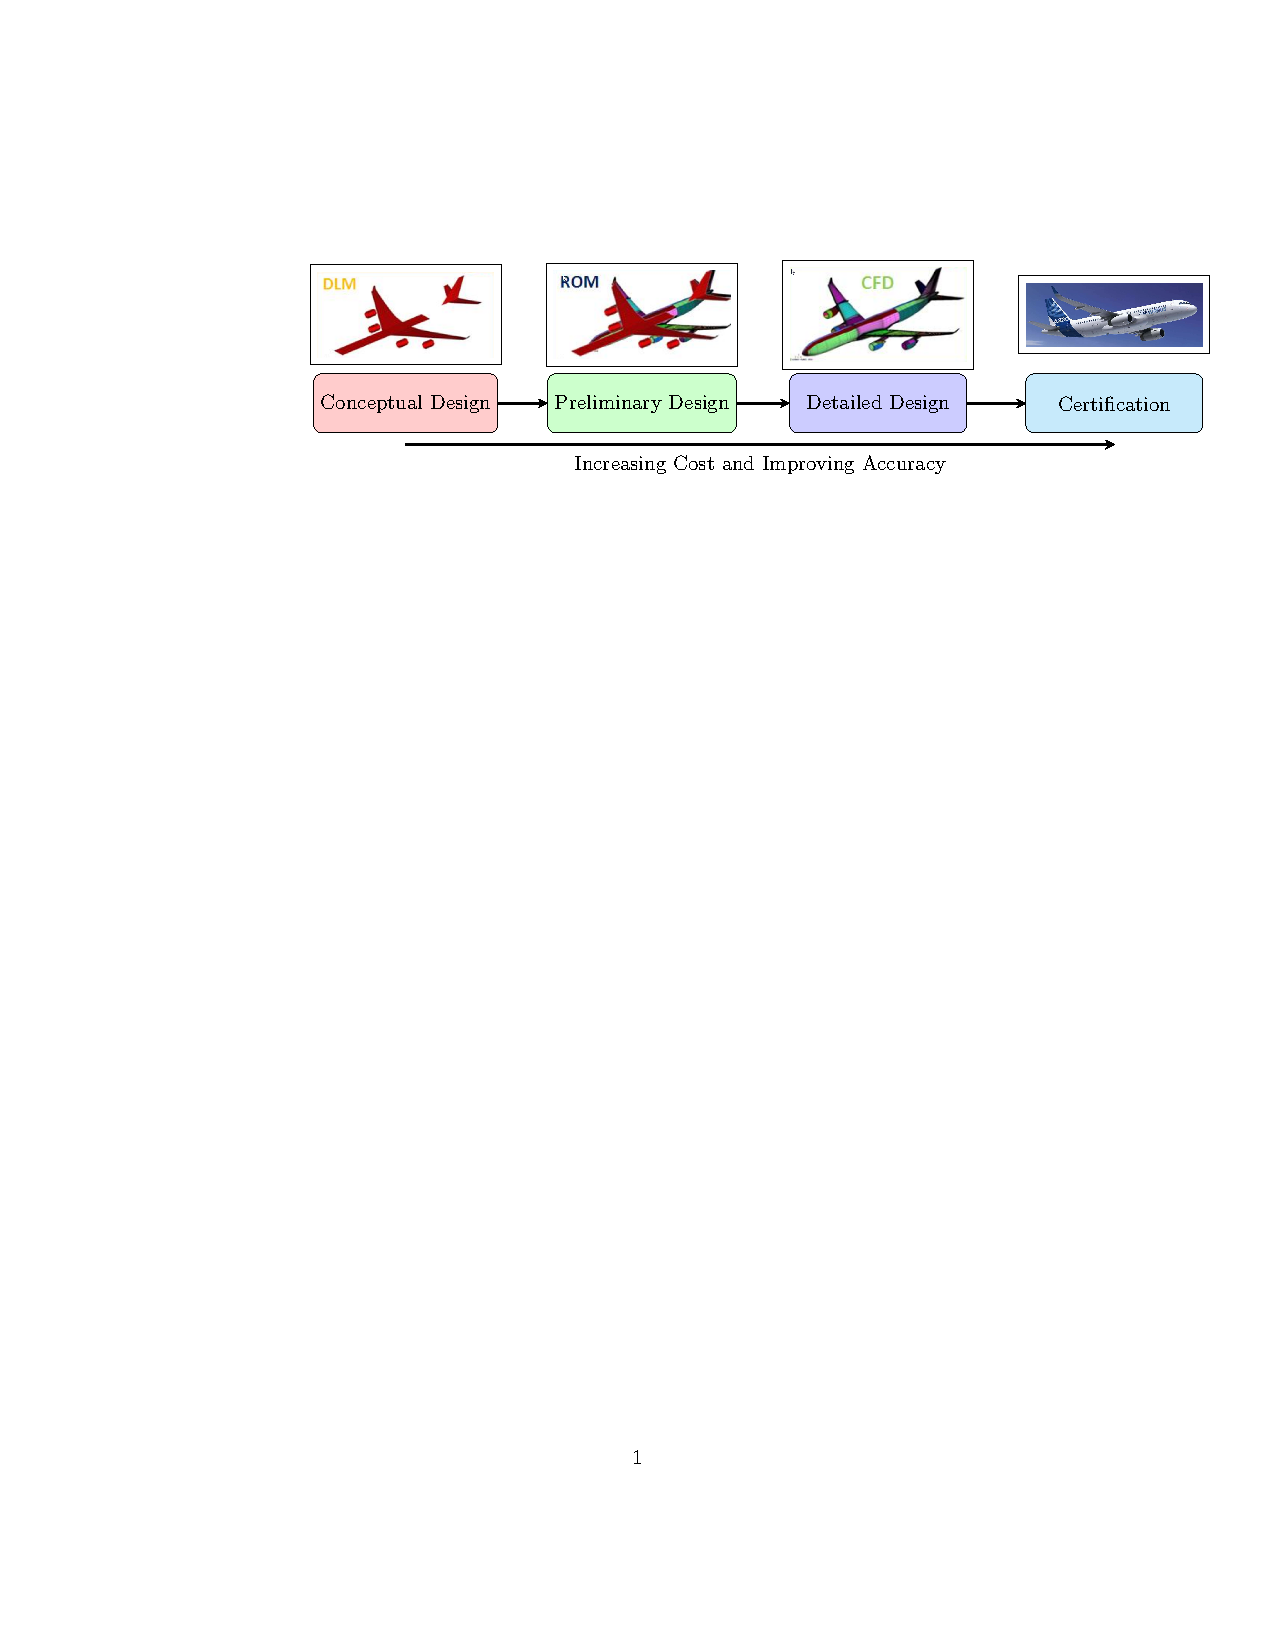
\includegraphics[clip, trim=4.5cm 19cm 0.5cm 4cm,width=0.95\textwidth]
    {flowchart/aircraftDesignCycleFlowChart}
  
  \caption{Phases of an aircraft design cycle}
\end{figure}

\section{Aircraft design cycle}\label{secSircraftDesignCycle}
\marginnote{\textsl{Design phases}}[1cm]
To simplify this process an aircraft design is broken down into several design phases (figure \ref{figPhasesOfAircraftDesign}). Each phase requires an ever increasing amount of predictions and fidelity. Preliminary design phase requires a few low-fidelity design trade-offs between major disciplines. Whereas, during detailed design phase, intensive intra-disciplinary and inter-disciplinary optimization's take place. Finally, during the flight-test and certification phase capability to predict real-time can provide significant gains in reducing the flight-test phase. These analyses cover large parts of flight envelope and require high-fidelity predictions. Hence the capability to accurately and quickly predict is an integral part of an aircraft design cycle \cite{raymer2012aircraft}. 

\marginnote{\textsl{Need for Speed}}[1cm]
In the last decade high-fidelity, physics based, non-linear mathematical simulations have become central to designing an aircraft. However, high-fidelity simulations are computationally expensive, this is the case for several Computational Fluid Dynamics (CFD) and Finite Element Method (FEM) based solvers. Due to this high cost high-fidelity simulations are launched only for a few carefully chosen configurations. This results in inefficient exploration of the the design space and thus a non-optimal design. A common strategy to speed up simulations is by reducing the physical complexity of the model to make quick predictions. As an example linear potential flows (simpler aerodynamic model), or coarser FEM meshes (simpler structural model) are regularly used during the preliminary design phase \cite{cummings2015applied}. While this is an acceptable practice during the preliminary design phase, during the detailed design phase physical complexity is needed to find a robust optimum design point \cite{raymer2012aircraft}.

\marginnote{\textsl{Need for accuracy}}[1cm]
Instead of approximating physical complexity, surrogate models\footnote{Surrogate models, learning algorithms and machine learning models will be used interchangeably throughout this manuscript} simplify mathematical complexity \cite{verveld2016reduced}. Surrogate models learn patterns between the input and output dataset and then are used to make predictions on the desired point. This property is very useful in quickly exploring the design space and finding a robust design point \cite{forrester2008engineering}. Moreover, surrogate models are commonly passed across disciplines to perform inter-disciplinary optimizations. For example, a loads department would prefer running a quick surrogate model over the costly CFD model while performing the load's loop.  

\marginnote{\textsl{Deduction vs Induction}}[1cm]
The main difference between the engineering design and surrogate modeling can be explained by the difference between deduction and induction \cite{domingos2012few} (figure \ref{fig:engineeringDesignVsSurrogateModelling}). Engineering design is deduction: where a very general formula is applied to a particular case (figure \ref{figDeduction}). The basics of Newtonian physics, when applied to a particular aircraft geometry, give inertial loads. The basics of aerodynamics, when applied to a particular set of aircraft geometry and aircraft states, give out aerodynamic pressures. Engineering design takes global rules and applies them to local configurations. Whereas, surrogate modeling is induction: it looks at local features and data, tries to find similarity measures between them and gives a global formula for the process (figure \ref{figInduction}). For example, an algorithm to detect faces in images will look at several images with and without faces, learn a facial pattern and make predictions on new images \cite{marszalek2007semantic}. We here see a possible complementary relationship between engineering design and machine learning; where engineering design needs models to generate data, machine learning needs data to generate models.

\begin{figure}[!ht]\label{fig:engineeringDesignVsSurrogateModelling}
  \centering
  \subfigure[Engineering design - Deduction: The figure shows an application of a general rule to a particular case.]
  {
    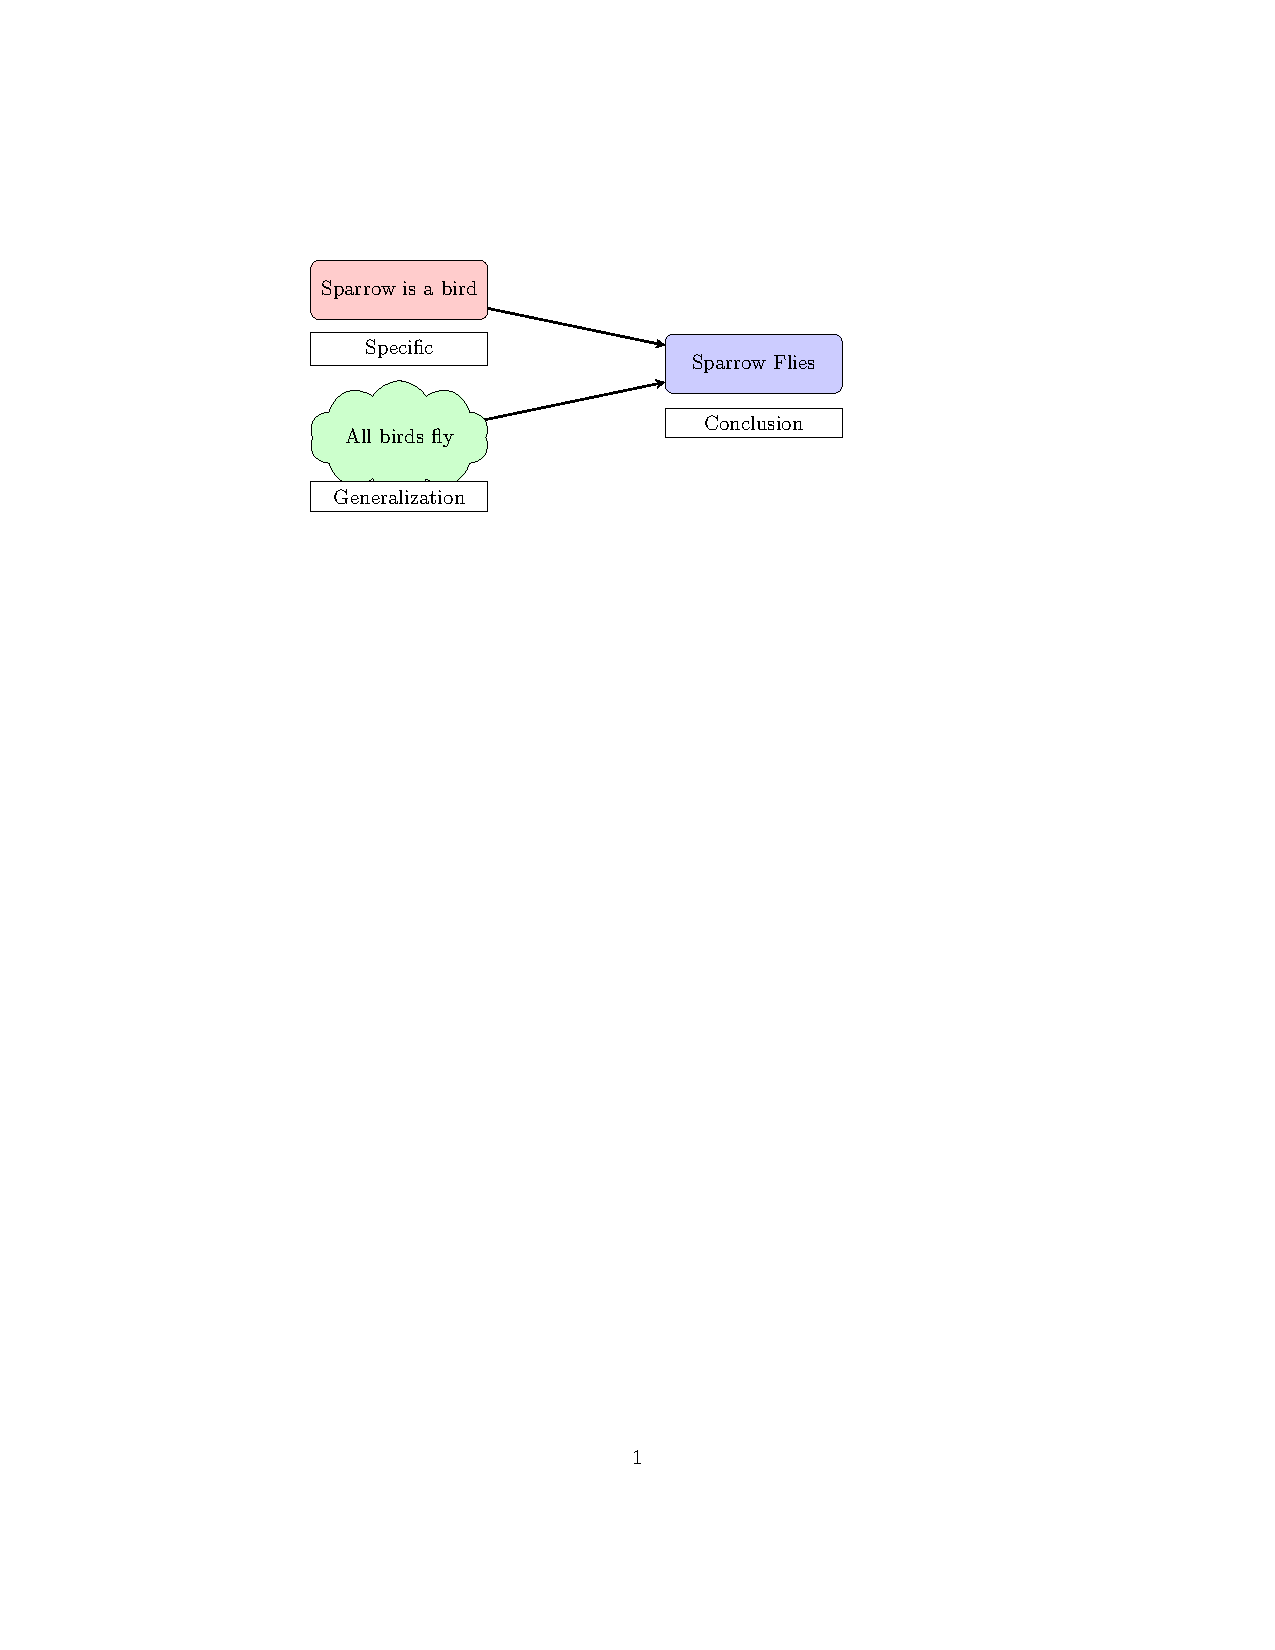
\includegraphics[clip, trim=4.5cm 19cm 4.5cm 4cm,width=0.45\textwidth]
    {flowchart/deduction}
    \label{figDeduction}
  }\quad
  \subfigure[Surrogate modelling - Induction: The figure shows how multiple examples can be used to infer underlying rules or patterns that govern the system.]
  {
    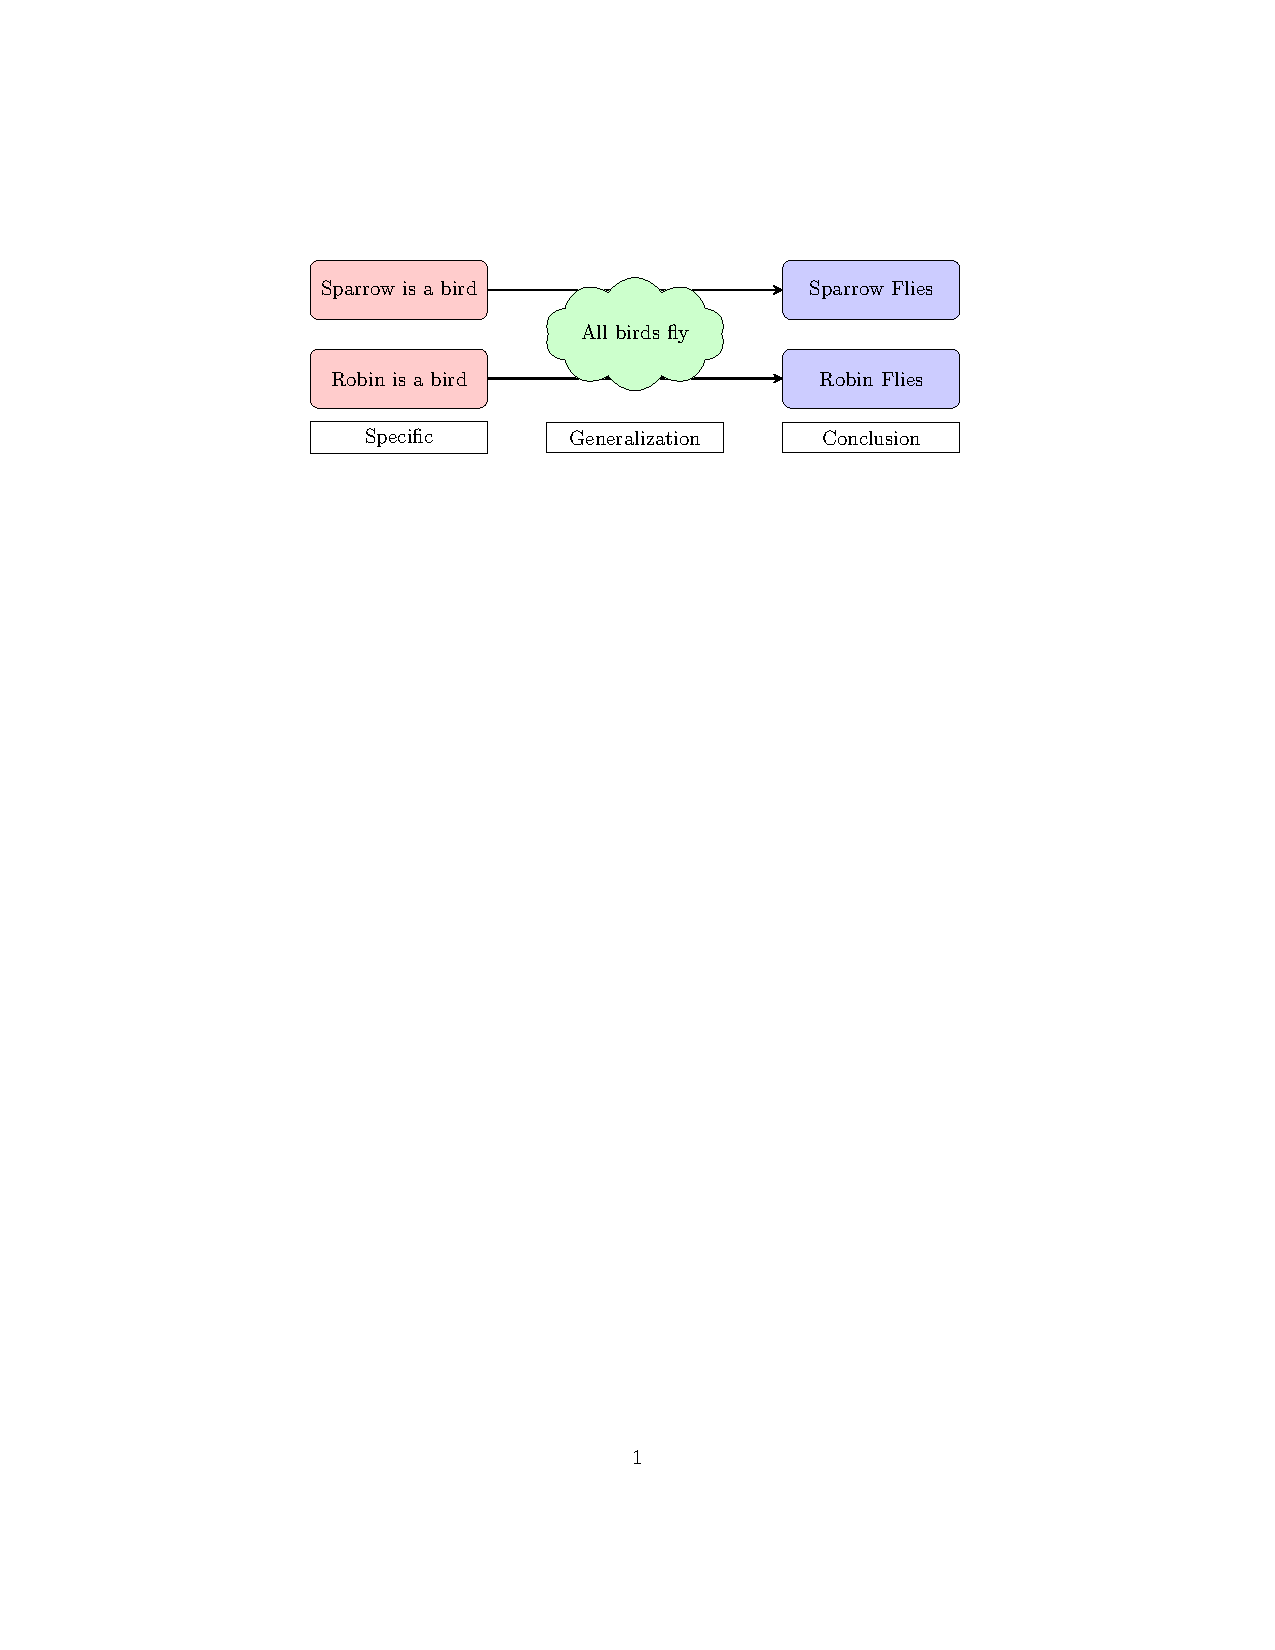
\includegraphics[clip, trim=4.5cm 20cm 4.5cm 4cm,width=0.45\textwidth]
    {flowchart/induction}
    \label{figInduction}
  }\quad
  \caption{Induction vs Deduction}
\end{figure}

\marginnote{\textsl{Developing faster models}}[1cm]
Since models are an integral part of any engineering design, model building in aircraft engineering was traditionally outsourced to research institutes. Researchers perform iterative experiments in a controlled environment and discover patterns between the physics of the system. For example, it took 200 years to iteratively develop the Gas law \footnote{\(Pressure \times Volume \approx numberOfMoles \times Temperature\)}, Boyle's law in 1600's found the relation between Pressure and Volume, Charle's Law in 1787 discovered the relationship between Volume and Temperature, while Gay-Lussac's Law in 1809 discovered the relationship between Pressure and Temperature \cite{clapeyron1834mémoire}. This is a rigorous and time-consuming method of developing models. Machine learning is a much more elegant method of building models. Using data and few basic assumptions, automatic models can be built between desired inputs and outputs. For example, while the first model of a neural network was proposed in 1950's \cite{kleene1951representation}, neural networks are today used daily for tasks such as tagging cat photos on facebook and converting speech to text\footnote{I wrote a fourth of this thesis using a text to speech software}. In this thesis, we wish to automatically build models for aircraft design tasks primarily to be used during the detailed design phase and certification phase. 


\section{Machine Learning}\label{secMachineLearning}
\marginnote{\textsl{Components of learning}}[1cm]
The core objective of learning algorithms is to find a transformation function between the inputs and outputs. There are three main components in a learning algorithm:
\begin{enumerate}
\item \textbf{Representation}: A learning algorithm starts with a family of functions. For example, a linear model is a family of linear functions, a trigonometric model defines a family of trigonometric functions. If an algorithm is not able to represent the actual function in its family of functions, it will find the closest function in its hypothesis space\footnote{The term family of functions, hypothesis space and representation will be used interchangeably throughout this manuscript}.
\item \textbf{Evaluation}: Some measure is needed to distinguish a good function from a bad function in the chosen hypothesis space. This measure is termed as evaluation; one example is the least squares error commonly used in many learning algorithms. 
\item \textbf{Optimization}: Finally, the algorithm iteratively searches in its hypothesis space to find the best possible function explaining the data. The choice of optimizer defines the speed of learning and is also important if there are multiple minima in the evaluation criteria.
\end{enumerate}

\marginnote{\textsl{Bias vs Variance}}[1cm]
Surrogate models suffer from the famous bias vs variance trade-off (figure \ref{figBiasVsVariance}), formalized by `Wolpert' in his famous "no free lunch theorem" \cite{wolpert1997no}. The constituent functions in a hypothesis space represent the bias or assumptions of the learning algorithm (eg. linear functions for linear regression). In the absence of sufficient assumptions, the family of functions in the search space becomes very large which leads to high variance or over-fitting in the surrogate model (figure \ref{subFigpredictionPoly15}). On the contrary, wrong bias means that the desired transformation function does not exist in the hypothesis space. In this case, the learning algorithm finds the closest function in its hypothesis space and leads to under-fitting (figure \ref{subFigpredictionPoly6}).

\begin{figure}[!ht]
  \centering
    \subfigure[{High-bias and low variance}]
  {
        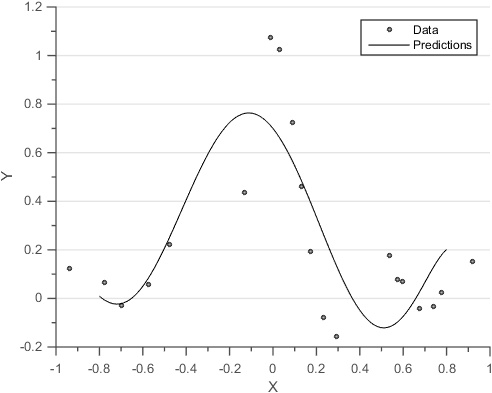
\includegraphics[width=0.29\textwidth]
        {images/predictionPoly6}
        \label{subFigpredictionPoly6}
  }\quad
\subfigure[{Low bias and High variance}]
  {
        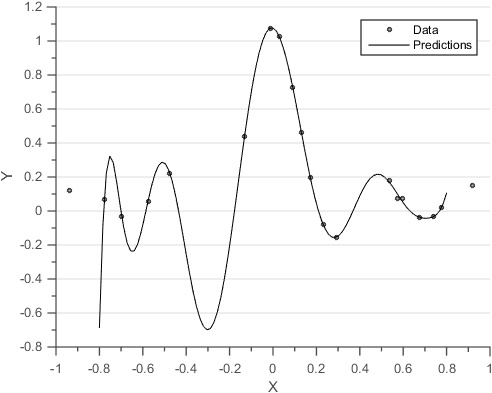
\includegraphics[width=0.29\textwidth]
        {images/predictionPoly15}
        \label{subFigpredictionPoly15}
  }\quad
  \subfigure[{Bias replaced with lots of data}]
  {
        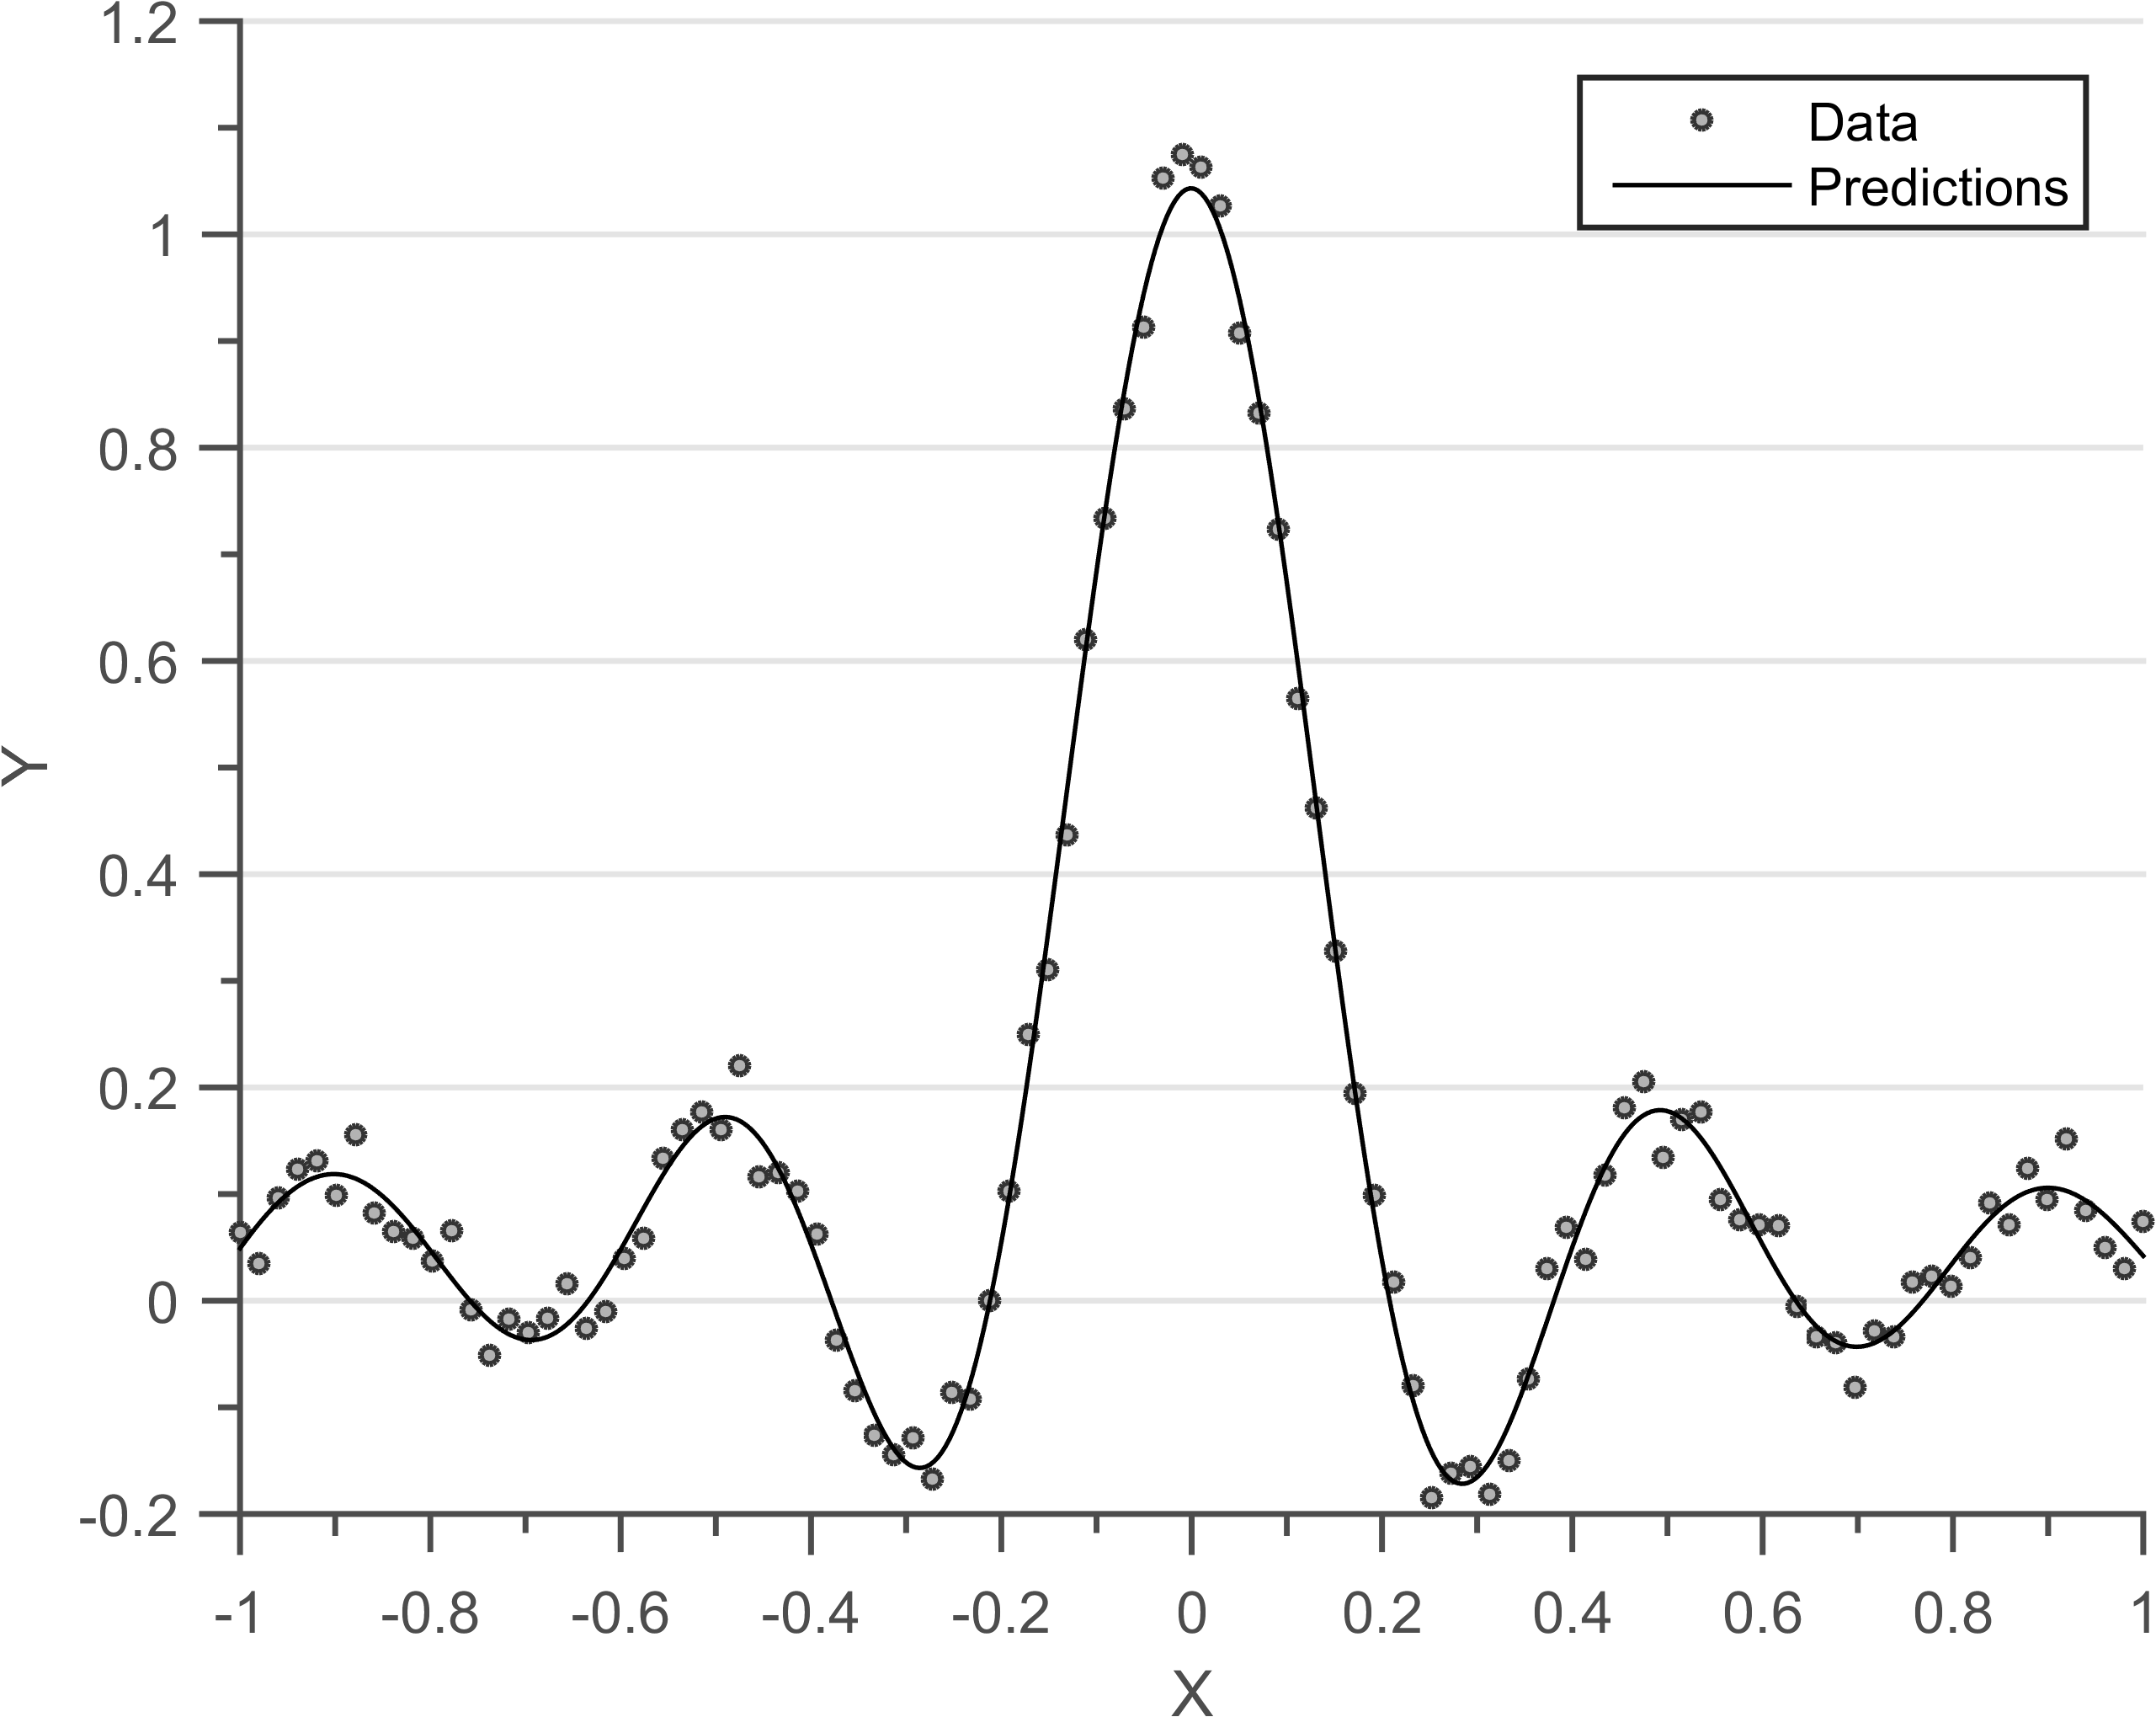
\includegraphics[width=0.29\textwidth]
        {images/posteriorSEInitialAtI100}
        \label{subFigposteriorSEInitialAtI100}
  }\quad
       \caption{Bias vs Variance trade-off}
       \label{figBiasVsVariance}
\end{figure}



\marginnote{\textsl{Soft and hard constraints}}[1cm]
One method to overcome this trade-off is by using lots and lots of data. Data acts as a hard constraint for learning algorithm, imagine a family of all possible continuous 2-dimensional functions in the range of $x \in [-1, 1]$ and $y \in [-1, 1]$. What will happen, given an observation $(x = 0, y = 0)$. All the functions that do not pass through this point will be eliminated, the new data point has basically reduced the possible family of functions. Whereas, bias acts as soft constraint, we can use the bias of linearity or smoothness to reduce our hypothesis space. Therefore, both bias and data help in reducing the hypothesis space\footnote{Bias can also be looked upon as distilled knowledge or patterns gained after interpreting huge amounts data}. Given access to more and more data we can progressively reduce the bias while learning models thereby relying more on true evidence. This is also the main concept behind deep learning, several layers of neural networks define a very large hypothesis space \cite{Goodfellow-et-al-2016, lecun2015deep}. 

Unfortunately, generating a huge amount of accurate data is a costly exercise in aircraft design e.g. a high fidelity CFD simulation runs for weeks \cite{murthy2014computational, jameson2012computational} and a flight-test campaign costs millions of euros \cite{fox2004test}. On another hand, we have a treasure trove of prior information about the physical systems, due to centuries of research and tinkering. We propose to build better machine learning models by integrating the time-tested available knowledge of physical systems with experimental data. 

\marginnote{\textsl{Contribution}}[1cm]
The main contribution of this thesis is to provide a framework on how to combine the prior knowledge from a physical system and add it to a learning algorithm. A model generated from merging of the two methodologies will be both consistent with the physics of the system and be quicker to evaluate. We integrate three types of prior knowledge by answering the following questions:
\begin{enumerate}
\item \textbf{Pattern}: How to add apriori information of a pattern in a learning algorithm? For example, given that shock is a discontinuous change in pressure, how to predict the position of shock on an airfoil (chapter \ref{chapStructureWithCovariance}). 
\item \textbf{Relationships}: How to add apriori information of relationships between measurements? For example given \(Loads = \int Pressures\), how to make a robust loads model when we measure both pressures and loads (chapter \ref{chapAddingEquationsInGP}).
\item \textbf{Simulation model}: How to merge apriori information of simulations with experiments? For example, given a simulation model and experimental data how to perform extrapolations on experimental data(chapter \ref{chapMultiTaskExtrapolation}). 
\end{enumerate}

To integrate the prior information we propose to use a Bayesian inference for model building. Bayesian inference is a method of statistical inference in which Bayes theorem is used to update an initial probability (prior) as more and evidence becomes available the final probability (posterior) gives our estimate. More specifically, we will use the Gaussian Processes (GP) Regression framework which is a subset of the Bayesian Inference algorithms to define prior information of physical systems. But, before deep diving into the details of GP let us have a look at a simple Bayesian Linear Regression algorithm.

\section{Bayesian Linear Regression}\label{secBayesianModelling}
Suppose we have access to a training set of observations (or outputs) \(Y = (y(x_{1}); \ldots ; y(x_{i}); \ldots ; y(x_{N}))\), evaluated at a set of known inputs \(X = (x_{1}; \ldots ; x_{i}; \ldots; x_{N})\), and we wish to predict \(y(x_{*})\) at a test input \(x_{*}\). The input and output can be multi-dimensional; \(x_{i} \in \mathbb{R}^{D_{inputs}}\) and \(y(x_{i}) \in \mathbb{R}^{D_{outputs}}\). The process of learning the transformation function \(f\) to make prediction at a new point is called as regression. In the following section we follow formulation for Bayesian Linear Regression provided by \cite{mackay2003information}.

\marginnote{\textsl{Basis functions}}[1cm]
A simple method to perform regression is by assuming a parametrized form of the function \(f\) and then minimizing the error between measurements and predictions to estimate the parameters of function. The function is written in terms of basis functions \(\phi(x)\). For example when \(\phi(x) = \{1, x\}\) we are performing linear regression, when \(\phi(x) = \{1, x, x^{2}, \ldots, x^{L}\}\) we are performing \(L^{th}\) order polynomial regression. We will focus on linear regression in this section and hence \(\phi(x) = \{1, x\}\).

\begin{equation}\label{eqBayesianLinearRegression}
f(x_{i}) = \begin{Bmatrix}
x^{0} & x^{1}
\end{Bmatrix}  \begin{Bmatrix}
w_{0}\\ 
w_{1}
\end{Bmatrix}
\quad \quad y(x_{i}) = f(x_{i}) + \epsilon
\end{equation}

\marginnote{\textsl{Likelihood}}[1cm]
Here, \(w\) are the parameters of the function. The measurements are corrupted by independent white noise \(\epsilon\), such that the noise is a random variable sampled from a white noise Gaussian with variance \(\sigma_{n}^{2}\)\footnote{\(\Pr[\epsilon] = \mathcal{N}(0, \sigma_{n} = \frac{1}{\sqrt{2\pi\sigma_{n}^{2}}}\exp^{-\frac{\epsilonç{2}}{2\sigma_{n}^{2}}}
)\)}. The above equations \ref{eqBayesianLinearRegression} can be combined to result in the likelihood \(\Pr[Y\mid X, w]\)

\begin{equation}\label{eqBayesianLikelihood}
\begin{aligned}
\Pr[Y \mid X, w]  & = \prod \Pr[y_{i}\mid x_{i}, w]\\
                & = \prod \mathcal{N}[x_{i}w , \sigma_{n}^{2}]\\
                & = \mathcal{N}(X w, \sigma_{n}^{2}I)    
\end{aligned}
\end{equation}

The notation \(\Pr[Y \mid X, w]\) symbolizes probability distribution of observations \(Y\) at the inputs \(X\) given the parameter \(w\). The notation \(\mathcal{N}[\mu , \Sigma]\) symbolizes a multi-variate Gaussian distribution for mean vector \(\mu\) and covariance matrix \(\Sigma\). 

\marginnote{\textsl{Prior}}[1cm]
While performing Bayesian inference we specify a prior distribution to encode our assumptions on the parameters before we look at the observations. For this case, we put a zero mean Gaussian prior on our weights.

\begin{equation}\label{eqBayesianPrior}
\Pr[w] = \mathcal{N}(0, \Sigma_{Prior})
\end{equation}

The prior distribution on \(w\) induces a prior distribution over functions parametrized by \(w\), effectively we are defining family of functions \((\Pr[f(x_{i})] = \mathcal{N}(0, x_{i}^{T}\Sigma_{Prior}x_{i}))\) by placing a prior distribution over \(w\). Once we have a prior distribution encoding our beliefs, we use Bayes rule to look at the observations and get a posterior distribution of parameters.

\begin{equation*}
posterior = \frac{likelihood \times prior}{marginal \quad likelihood}
\end{equation*}
\begin{equation}\label{eqBayesRule}
\Pr[w \mid Y, X] = \frac{\Pr[Y \mid X, w] \times \Pr[w]}{\Pr[Y \mid X]}
\end{equation}

\marginnote{\textsl{Marginal Likelihood}}[1cm]
The \textsl{marginal likelihood} is a normalization constant, for more details please refer to section \ref{secHyperParameter}. After, using the equation \ref{eqBayesianLikelihood}, \ref{eqBayesianPrior} and \ref{eqBayesRule} we can get the posterior distribution of weights as:

\begin{equation}\label{eqBayesianPosterior}
\Pr[w \mid Y, X]  = \mathcal{N}\left ( \frac{1}{\sigma_{n}^{2}} A^{-1}X Y , A^{-1} \right )
\end{equation}

Here, \(A = \sigma_{n}^{-2}XX^{T} + \Sigma_{Prior}^{-2}\). Thus the posterior distribution for function \(f\) at test point \(x_{*}\) becomes:

\begin{equation}\label{eqBayesianFunctionalPosterior}
\Pr[f \mid x_{*}, X, y]  = \mathcal{N}\left ( \frac{1}{\sigma_{n}^{2}} x_{*}A^{-1}XY , x_{*}^{T}A^{-1}x_{*} \right )
\end{equation}

\marginnote{\textsl{Posterior}}[1cm]
The mean \(\frac{1}{\sigma_{n}^{2}} x_{*}A^{-1}XY\) can be used as a prediction at the test point \(x_{*}\), while the variance is a measure of uncertainty for this prediction. We can thus obtain the prediction \(f(x_{*})\), using a prior set of beliefs (equation \ref{eqBayesianPrior}) and updating those beliefs using observations. While the Bayesian Linear Regression framework provides an opportunity to encode prior assumptions in terms of distributions of the parameters. A much more elegant and expressive method is by using Gaussian Processes to perform regression. Gaussian Processes are a distribution over functions and hence enable us to encode prior knowledge directly in the functional space. 

\marginnote{\textsl{Non-parametric models}}[1cm]
Learning algorithms are mainly divided into two main types. The first is defined by parametric models which can only represent a limited hypothesis space. They use parameters to describe the function between input and output domain. For example the weight parameters \(w\) in Bayesian Linear Regression. The second are non-parametric models whose hypothesis space grows with the size of data. Non-parametric models use data to represent functions, Gaussian Process Regression is a type of non-parametric model. One can imagine a non-parametric model like a stretched rubber sheet: whenever it sees data it deforms accordingly to compensate for the new data point. Hence the more data it sees the more it starts mimicking the actual function. 

\marginnote{\textsl{Gaussian Process}}[1cm]
Gaussian Process or Kriging was first used in the context of Geo-statistics research by Daniel Krige \cite{krige1951statistical}, this was later formalized by Matheron in his seminal work "Principals of Geo-statistics" \cite{matheron1963principles}. Recently, interest in the Gaussian Process (GP) grew in the machine learning community from neural networks research. It was shown that a Bayesian neural network becomes a Gaussian process as the number of neurons tends to infinity \cite{neal2012bayesian}. Gaussian processes are probabilistic distributions over functions, which provide a Bayesian non-parametric approach to smoothing and interpolation. A Gaussian Process can be fully parameterized by its mean and covariance function. More generally, a Gaussian Process is a method to probabilistically define a family of functions, chapter \ref{chapGp} expands GP in more detail. 

\section{Outline}\label{secOutline}
This thesis is divided into three main parts, each part is then divided into individual chapters and their constituent sections. This part sets up the prerequisites required to understand the concepts introduced in the next two parts. The first chapter demonstrates the need for performing regression in aircraft design tasks and describes a very basic Bayesian Linear Regression scheme. 

\marginnote{\textsl{Chapter \ref{chapGp}}}[1cm]
Chapter \ref{chapGp} shows the key processes involved in a GP regression framework. GPs as distributions over functions have a rich history in geo-statistics and machine learning. The second chapter heavily draws ideas from \cite{krige2015statistical, matheron1963principles} of the geo-statistics community and \cite{Stein1999Springer, kennedy2000predicting, Rasmussen2005, mackay2003information} of the machine-learning community, showing a process flow of how to perform regression using GPs. The remaining chapter unfolds as follows, section \ref{secPrior} describes the key constituents of a GP and how to draw random functions from a GP. Section \ref{secPosterior} describes how to perform prediction in presence and absence of measurement noise. Section \ref{secHyperParameter} introduces marginal likelihood as a form of evaluation method to automatically choose hyper-parameters. 

\marginnote{\textsl{Chapter \ref{chapSparseGPRegression}}}[1cm]
Chapter \ref{chapSparseGPRegression} deals with the problem of scaling GP regression to massively many points. Traditional GPs are computationally infeasible on a standard laptop if the number of data points increase \(\mathcal{O}(10^4)\). There exist two main methods to scale a GP regression, one using reduced set of inducing points while another based on mixture of experts methodology. This chapter draws heavily from the works of \cite{quinonero2005unifying, seeger2003fast, Snelson06sparsegaussian, Titsias09variationallearning} for the approximation method of inducing points and \cite{cao2014generalized, tresp2000bayesian, chen2009bagging, deisenroth2015distributed} for the approximation method of mixture of experts, please refer to the individual publications for more detail. We demonstrate the limitations and capabilities of both the methods on a toy dataset, giving directions to choosing optimal parameters and extracting the best possible result.  

\textbf{Description of the other two parts}

%%% Local Variables: 
%%% mode: latex
%%% TeX-master: "isae-report-template"
%%% End: 

\chapter{Gaussian Process Regression}
\label{chapGp}

Suppose we perform a simulation or experiment on an input point $x_{j} \in \mathbb{R}^{D_{inputs}}$and measure an output $y_{j} \in \mathbb{R}$. In this chapter we assume that the input is $D_{inputs}$ dimensional and the output is one dimensional. We can thus have a data set of $N$ observations, $\{\mathcal{D} = (x_{j}, y_{j}) | j \in [1; N] \}$. The full input and output vectors can be denoted as $X = \{x_{1}; x_{2}; \ldots ; x_{N}\}$ and $Y = \{y_{1}; y_{2}; \ldots ; y_{N}\}$ such that $X \in \mathbb{R}^{N \times P}$ and $Y \in \mathbb{R}^{N }$. Given this data we are interested in making predictions for new input points $x_{*}$ \footnote{Also called as test point, prediction point or target point.}that are not present in our series of experiments. This means that we need to use out training data and learn, the true physical process  $f(x)$ that generates our data set.

As discussed in the previous chapter, to learn the governing function $f(x)$ we first start with a family of functions. Gaussian Process (GP) can be used to probabilistically define a family of functions. More formally, a GP is a distribution over functions such that any finite set of function values $[f(x_{1}), f(x_{2}), \ldots, f(x_{N})]$ have a joint Gaussian distribution \cite{rasmussen2006gaussian}. 

\marginnote{\textsl{Infinite dimensional random vector}}[1cm]
While a normal distribution describes a scalar random variable, example $X \sim \mathcal{N}(0, 1)$ defines a Gaussian variable with mean $0$ and variance $1$. A multi variate distribution defines a vector of random variables, for example $\{X\} \sim \mathcal{N}(\{0, 0\}, [1, 0; 0, 1])$ defines a Gaussian vector with mean $\{0, 0\}$ and covariance $[1, 0; 0, 1]$. A GP is the extension of this concept in the functional space. We can also think of a function as an infinite dimensional vector, each entry in the vector specifying the function value $f(x)$ at a particular point $x$ \footnote{Yes blew my mind as well!}. 

\marginnote{\textsl{Mean}}[1cm]
A GP model before conditioning on data can be completely parameterized by its mean

\begin{equation}\label{eq:meanGP}
\mathbf{E}[f(x)] = m(x)
\end{equation}

\marginnote{\textsl{Covariance}}[1cm]
and its covariance function also called a kernel. In the context of the GPs a kernel is a measure of similarity between pairs of functional values $(f(x))$ evaluated at input points , often involving an inner product of basis functions $\phi(x)$ \cite{bishop2006pattern}. Please refer to chapter \ref{chapBasicCovarianceKernels} for a more detailed insight into kernels.   \footnote{The terms covariance functions, kernel and kernel functions will be used interchangeably during the reminder of this thesis}:

\begin{equation}\label{eq:covarianceGP}
Cov[f(x) - m(x), f(x') - m(x')] = k(x_{1}, x_{2})
\end{equation}

We can formally write the probability of the function $f$ as:

\begin{equation}\label{equationGPdefinition}
\Pr[f(x)] = GP(m(x), k(x_{1}, x_{2}))
\end{equation}

The notation $\Pr(f( x))$ symbolizes probability distribution of function $f$ at the inputs $x$. A function randomly drawn from a GP yields a random function around the mean function $m(x)$ and of the shape as defined by covariance function $k(x_{1}, x_{2})$. 

\marginnote{\textsl{Tractable}}[1cm]
Performing inference on an infinite dimensional vector (function) can be a computationally intensive task. Thankfully, due to the marginalization property of Gaussians, if we ask for properties of the function at a finite number of points, then  GP will give us the same answer if we ignore the infinitely many other points. In other words any finite set of function values $[f(x_{1}), f(x_{2}), \ldots, f(x_{N})]$ have a joint Gaussian distribution in GP (also the  definition of GP). This property means that GP specified in equation \ref{equationGPdefinition} also specifies equation \ref{equationGPMarginalizationProperty}. This makes GPes computationally tractable, one of the major benefits of GP. 


\begin{equation}\label{equationGPMarginalizationProperty}
\Pr\left [ \begin{matrix}
f(x_{1})
\\ f(x_{2})
\end{matrix} \right ] = \mathcal{N}\left (\left [ \begin{matrix}
m(x_{1})
\\ m(x_{2})

\end{matrix} \right ] , \left [ \begin{matrix}
k(x_{1}, x_{1}) & k(x_{1}, x_{2})\\ 
k(x_{2}, x_{1}) & k(x_{2}, x_{2})
\end{matrix} \right ] \right )
\end{equation}

While performing regression in a GP framework we first define a family of functions also called prior (section \ref{secPrior}). The next step involves taking observations and eliminating all the functions in our prior which do not obey the observations, this step gives us the posterior mean and variance (section \ref{secPosterior}). Finally, we can further improve our predictions by fine-tuning our hyper-parameters (section \ref{secHyperParameter}).

\section{Prior} \label{secPrior}
In the Bayesian framework, a prior is a probability distribution before looking at any evidence. In the context of a GP Regression, this is provided by the mean and covariance function. 

\subsection{Hyperparameters}
Both mean and covariance functions are specified by a set of hyper-parameters $\theta$. The hyper-parameters are very similar to weight parameter ($w$) during Bayesian Linear Regression (section \ref{secBayesianModelling}), these are the parameters of the GP. Selecting a prior in GP boils down to choosing an appropriate functional form of the mean and covariance matrix and then choosing the hyper-parameters of the prior \cite{duvenaud2013structure}. 

Automatically, predicting the values of hyper-parameters is important to choose a good prior. We will look at how to choose good hyper-parameters in section \ref{secHyperParameter}. 

\subsection{Mean function}\label{subSecCH2MeanFunction}
The mean function $m(x)$ of a GP represents its trend. In Universal Kriging, we usually choose a mean function of the form $m(x) = \phi(x)^{T}\theta$, with $\phi(x) = (\phi_{1}(x), \ldots , f_{p}(x))$ being a vector of basis functions, generally including a constant function and $\theta \in \mathbb{R}^{p}$ is a vector of hyper-parameters \cite{matheron1963principles}. In Simple Kriging we assume a constant mean function $m(x) = \theta$.

\marginnote{\textsl{Zero mean}}[1cm]
Without loss of generality, we can assume the mean function to be zero everywhere, since uncertainty about the mean function can be taken into account by adding an extra term to the covariance function (Chapter \ref{chapBasicCovarianceKernels}).  

\begin{equation}\label{equationMeanZeroGPdefinition}
\Pr[f(x)] = GP(0 , k(x_{1}, x_{2}, \theta))
\end{equation}

We assume a zero mean prior through out this section. After accounting for the zero mean, the GP model can be completely parametrized by the kernel. Hence the problem of learning in a GP is exactly the problem of finding suitable properties of the covariance function \cite{rasmussen2006gaussian} (equation \ref{equationMeanZeroGPdefinition}). 


\subsection{Covariance function}\label{subSecCH2Covariance}
The covariance function is a positive definite kernel, such that for any $a_{i} \in \mathbb{R}$ equation \ref{equationPDKernel} holds \cite{Stein1999Springer}.

\begin{equation}\label{equationPDKernel}
\sum_{i=1}^{N}\sum_{j=1}^{N}a_{i}a_{j}k(x,x') \geq 0
\end{equation}

A popular choice of covariance function is a Squared Exponential (SE) function (equation \ref{eqnSquaredExponential}), because it defines a family of highly smooth (infinitely differentiable) non-linear functions as shown in figure \ref{figGPPriors}.

\begin{equation}\label{eqnSquaredExponential}
k_{SE}(x_{1}, x_{2}, \theta) = \theta_{amplitude}^2exp[-\frac{d^2}{2\theta_{lengthScale}^2}]
\end{equation}

\marginnote{\textsl{SE kernel}}[1cm]
For the case of the SE kernel the hyper-parameters $(\theta = [\theta_{amplitude}, \theta_{lengthScale}])$ are; amplitude $(\theta_{amplitude})$ which defines average distance from mean and the length scale $(\theta_{lengthScale})$ which defines the smoothness of functions. Here, $d$ defines the absolute distance between points $|x-x'|$. Covariance functions which are purely a function of distance $d$ are called as isotropic stationary functions. These covariance functions remains unchanged if the points $x_{1}, x_{2}$ are rotated or translated. Hence a family of functions defined by stationary kernels will have similar local features throughout the input domain. 

\marginnote{\textsl{Length-Scale}}[1cm]
When $x$ tends to $x'$ then $k(x_{1}, x_{2})$ approaches $\theta_{amplitude}^{2}$, this means that $f(x)$ is highly correlated with $f(x')$. This is a good characteristic for smooth functions, since points in the neighbourhood must be alike. If $x$ is far away from  $x'$ then $k(x_{1}, x_{2})$ tends to zero, this means that far away points are loosely correlated. Hence, far off observations will have negligible effect while performing interpolations. How fast or slow the covariance decreases with distance depends on the length scale parameter $\theta_{lengthScale}$, smaller length-scale means a faster moving function. In general we cannot extrapolate more than $\theta_{lengthScale}$ units from the closest data-point \cite{duvenaud-thesis-2014}. 

\subsection{Sampling functions from GP priors}\label{subSecSamplingFunctionsGPPrior}
To have a look at the constituent functions in a prior we can randomly sample functions from the GP. Since any finite set of set of function values have a joint Gaussian distribution in a GP. To draw random functions from a GP we choose $N*$ input points $X_{*} = \{x_{1*}; x_{2*}; \ldots ; x_{N*}\}$ and write corresponding mean vector $m(X_{*})$ and covariance matrix $K(X_{*}, X_{*} )$ \footnote{The covariance matrix is also called the Gram matrix} using equation \ref{equationGPMarginalizationProperty} and \ref{eqnSquaredExponential}. We then generate a random Gaussian vector $f(X_{*})$ for this multi-variate Gaussian (equation \ref{equationMeanZeroGPdefinition}) and plot the generated values as a function of inputs $X_{*}$. 

\begin{equation}\label{eqnCovMatrixSquaredExponential}
K(X_{*}, X_{*} ) = \left [ \begin{matrix}
k(x_{1*}, x_{1*}) & k(x_{1*}, x_{2*}) & \ldots & k(x_{1*}, x_{N*})
\\ k(x_{2*}, x_{1*}) & k(x_{2*}, x_{2*}) & \ldots & k(x_{2*}, x_{N*})
\\ \vdots & \vdots & \ddots & \vdots
\\ k(x_{N*}, x_{1*}) & k(x_{N*}, x_{2*}) & \ldots & k(x_{N*}, x_{N*})
\end{matrix} \right ] 
\end{equation}

Figure \ref{figGPCovarianceMatrix} shows the covariance matrix for Standard Exponential kernel with different hyper-parameters at the input points $X^{*} = \{[0:0.02:1]\}$. The SE kernel of figure \ref{subFigcovSEmatrix_1} has a lower length-scale than figure \ref{subFigcovSEmatrix_2}. Note, how the covariance values are more spread out for figure \ref{subFigcovSEmatrix_2}.

\begin{figure}[!ht]
  \centering
    \subfigure[{Covariance matrix for a Standard Exponential (SE) Kernel with $(\theta = [1, 0.2])$ at the input points $X^{*} = \{[0:0.02:1]\}$. }]
  {
        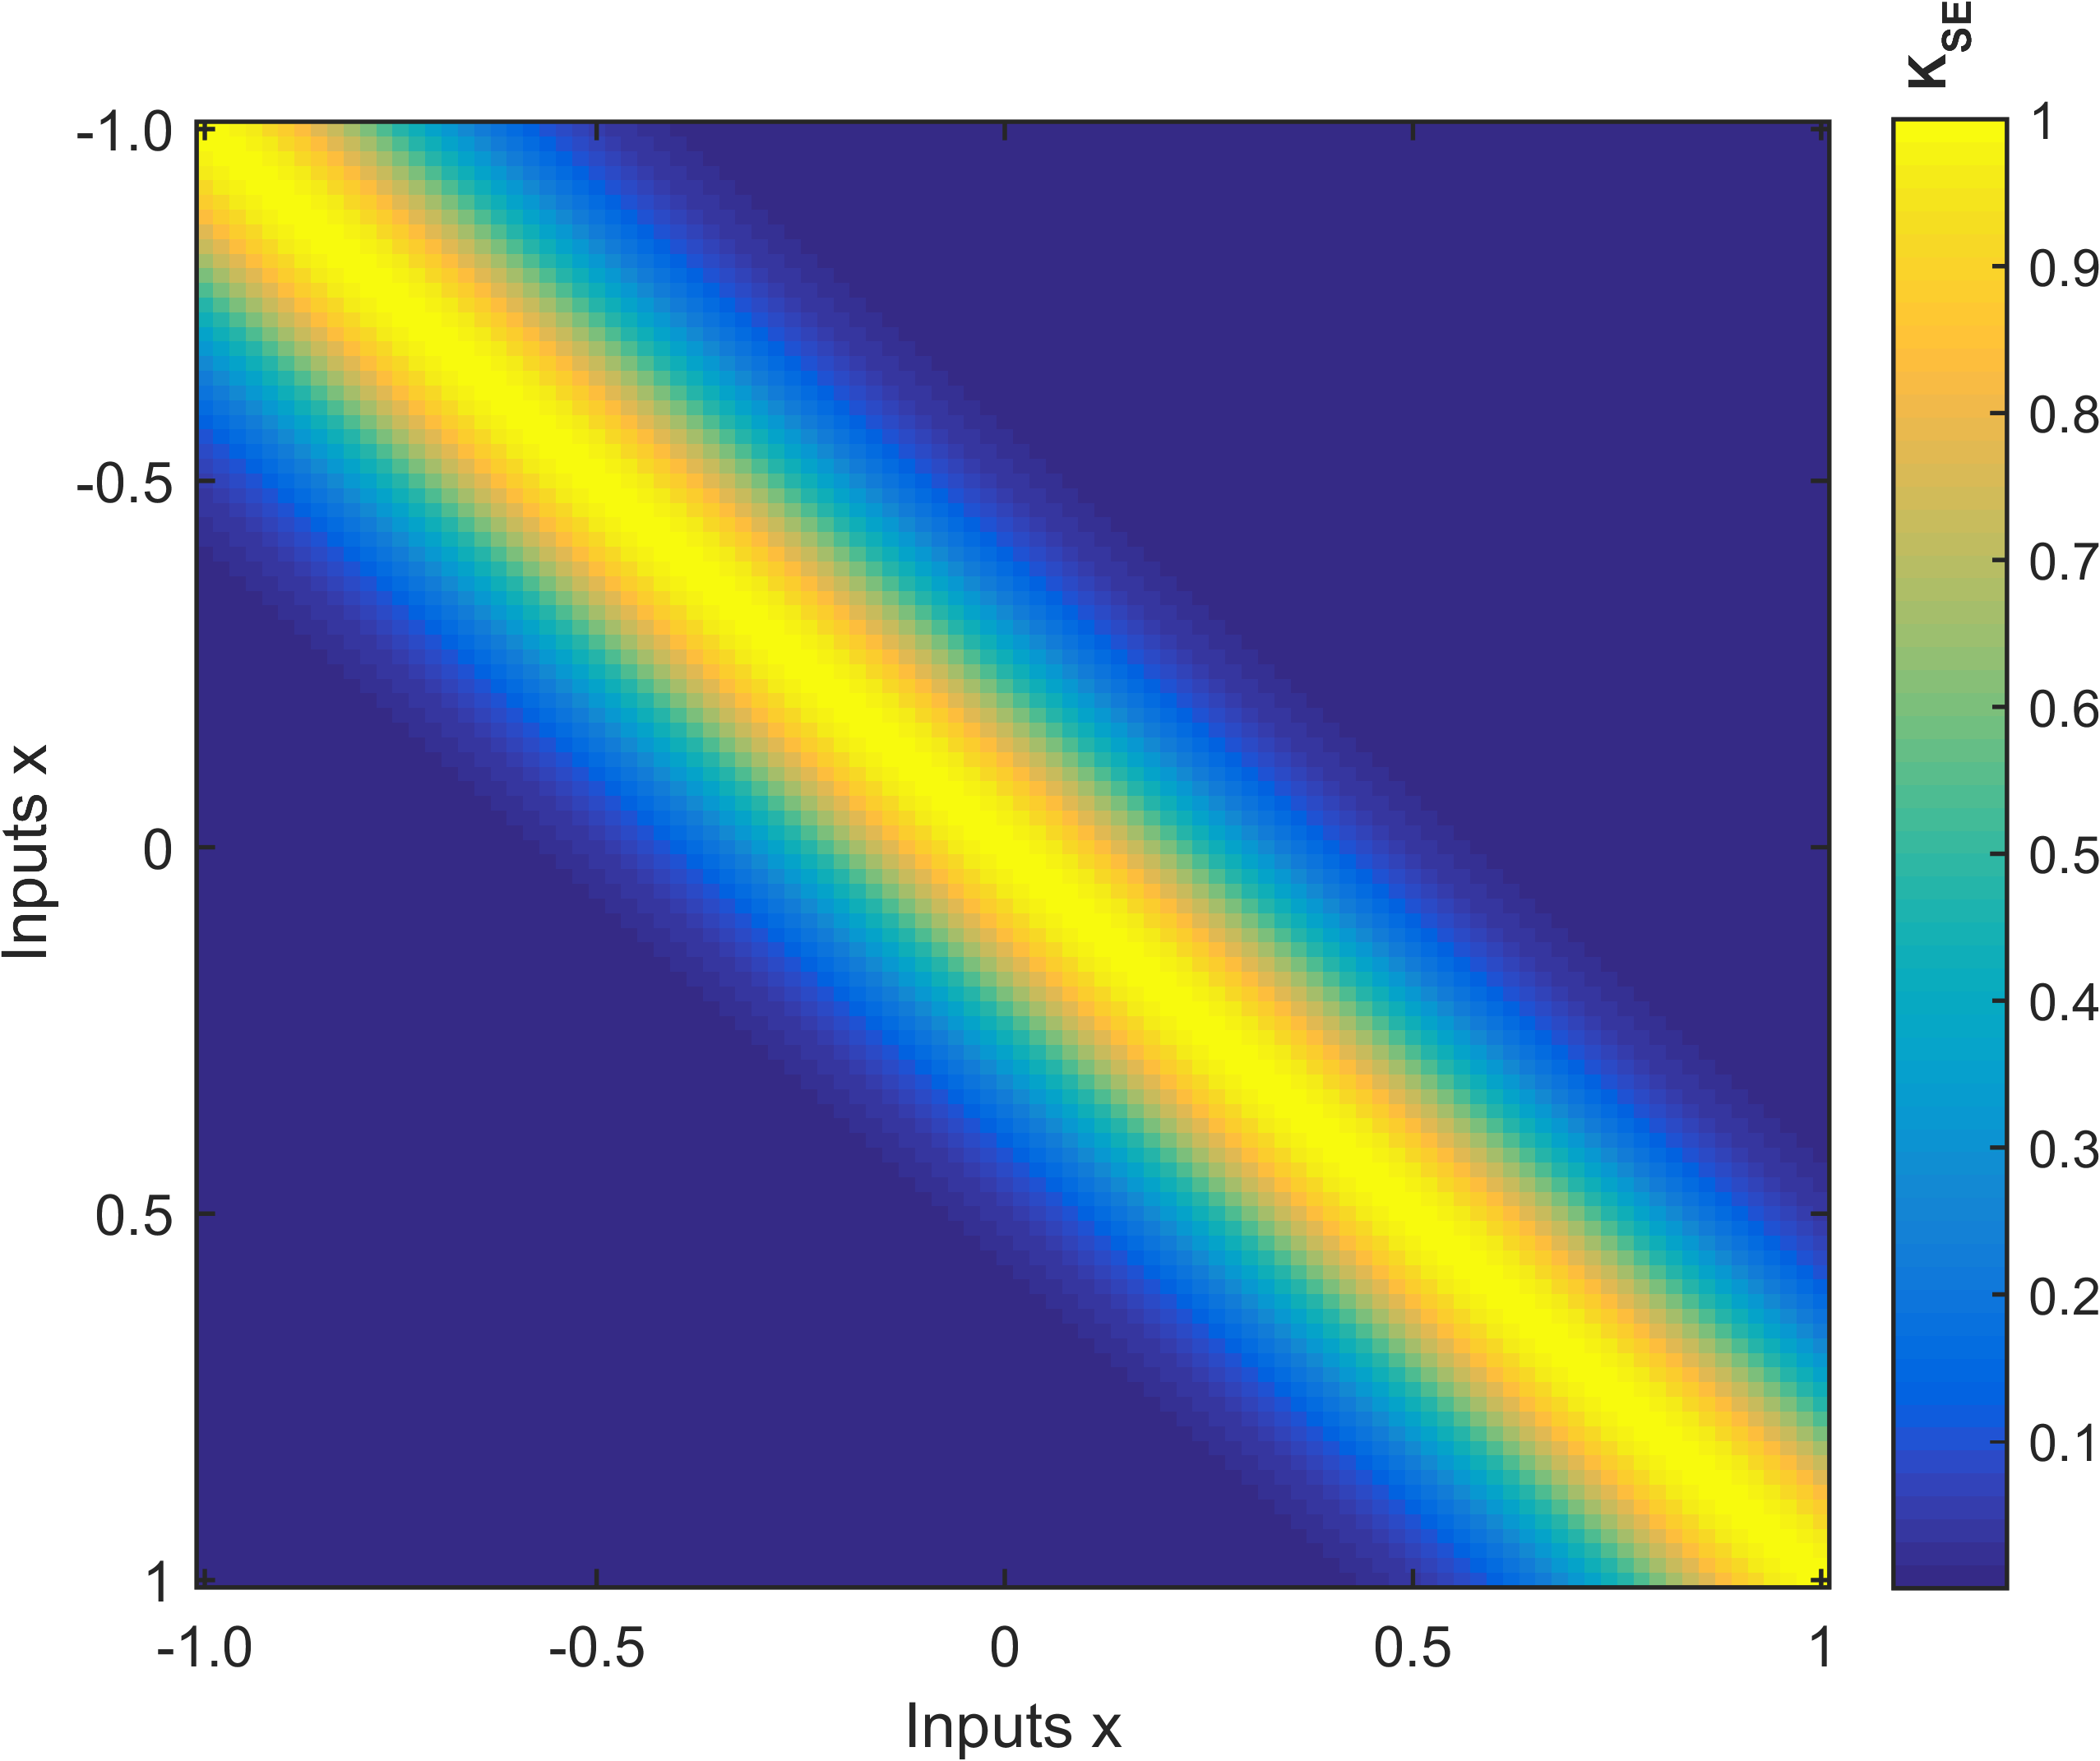
\includegraphics[width=0.45\textwidth]
        {images/covSEmatrix_1}
        \label{subFigcovSEmatrix_1}
  }\quad
\subfigure[{Covariance matrix for a Standard Exponential (SE) with $(\theta = [1, 0.5])$ at the input points $X^{*} = \{[0:0.02:1]\}$}]
  {
        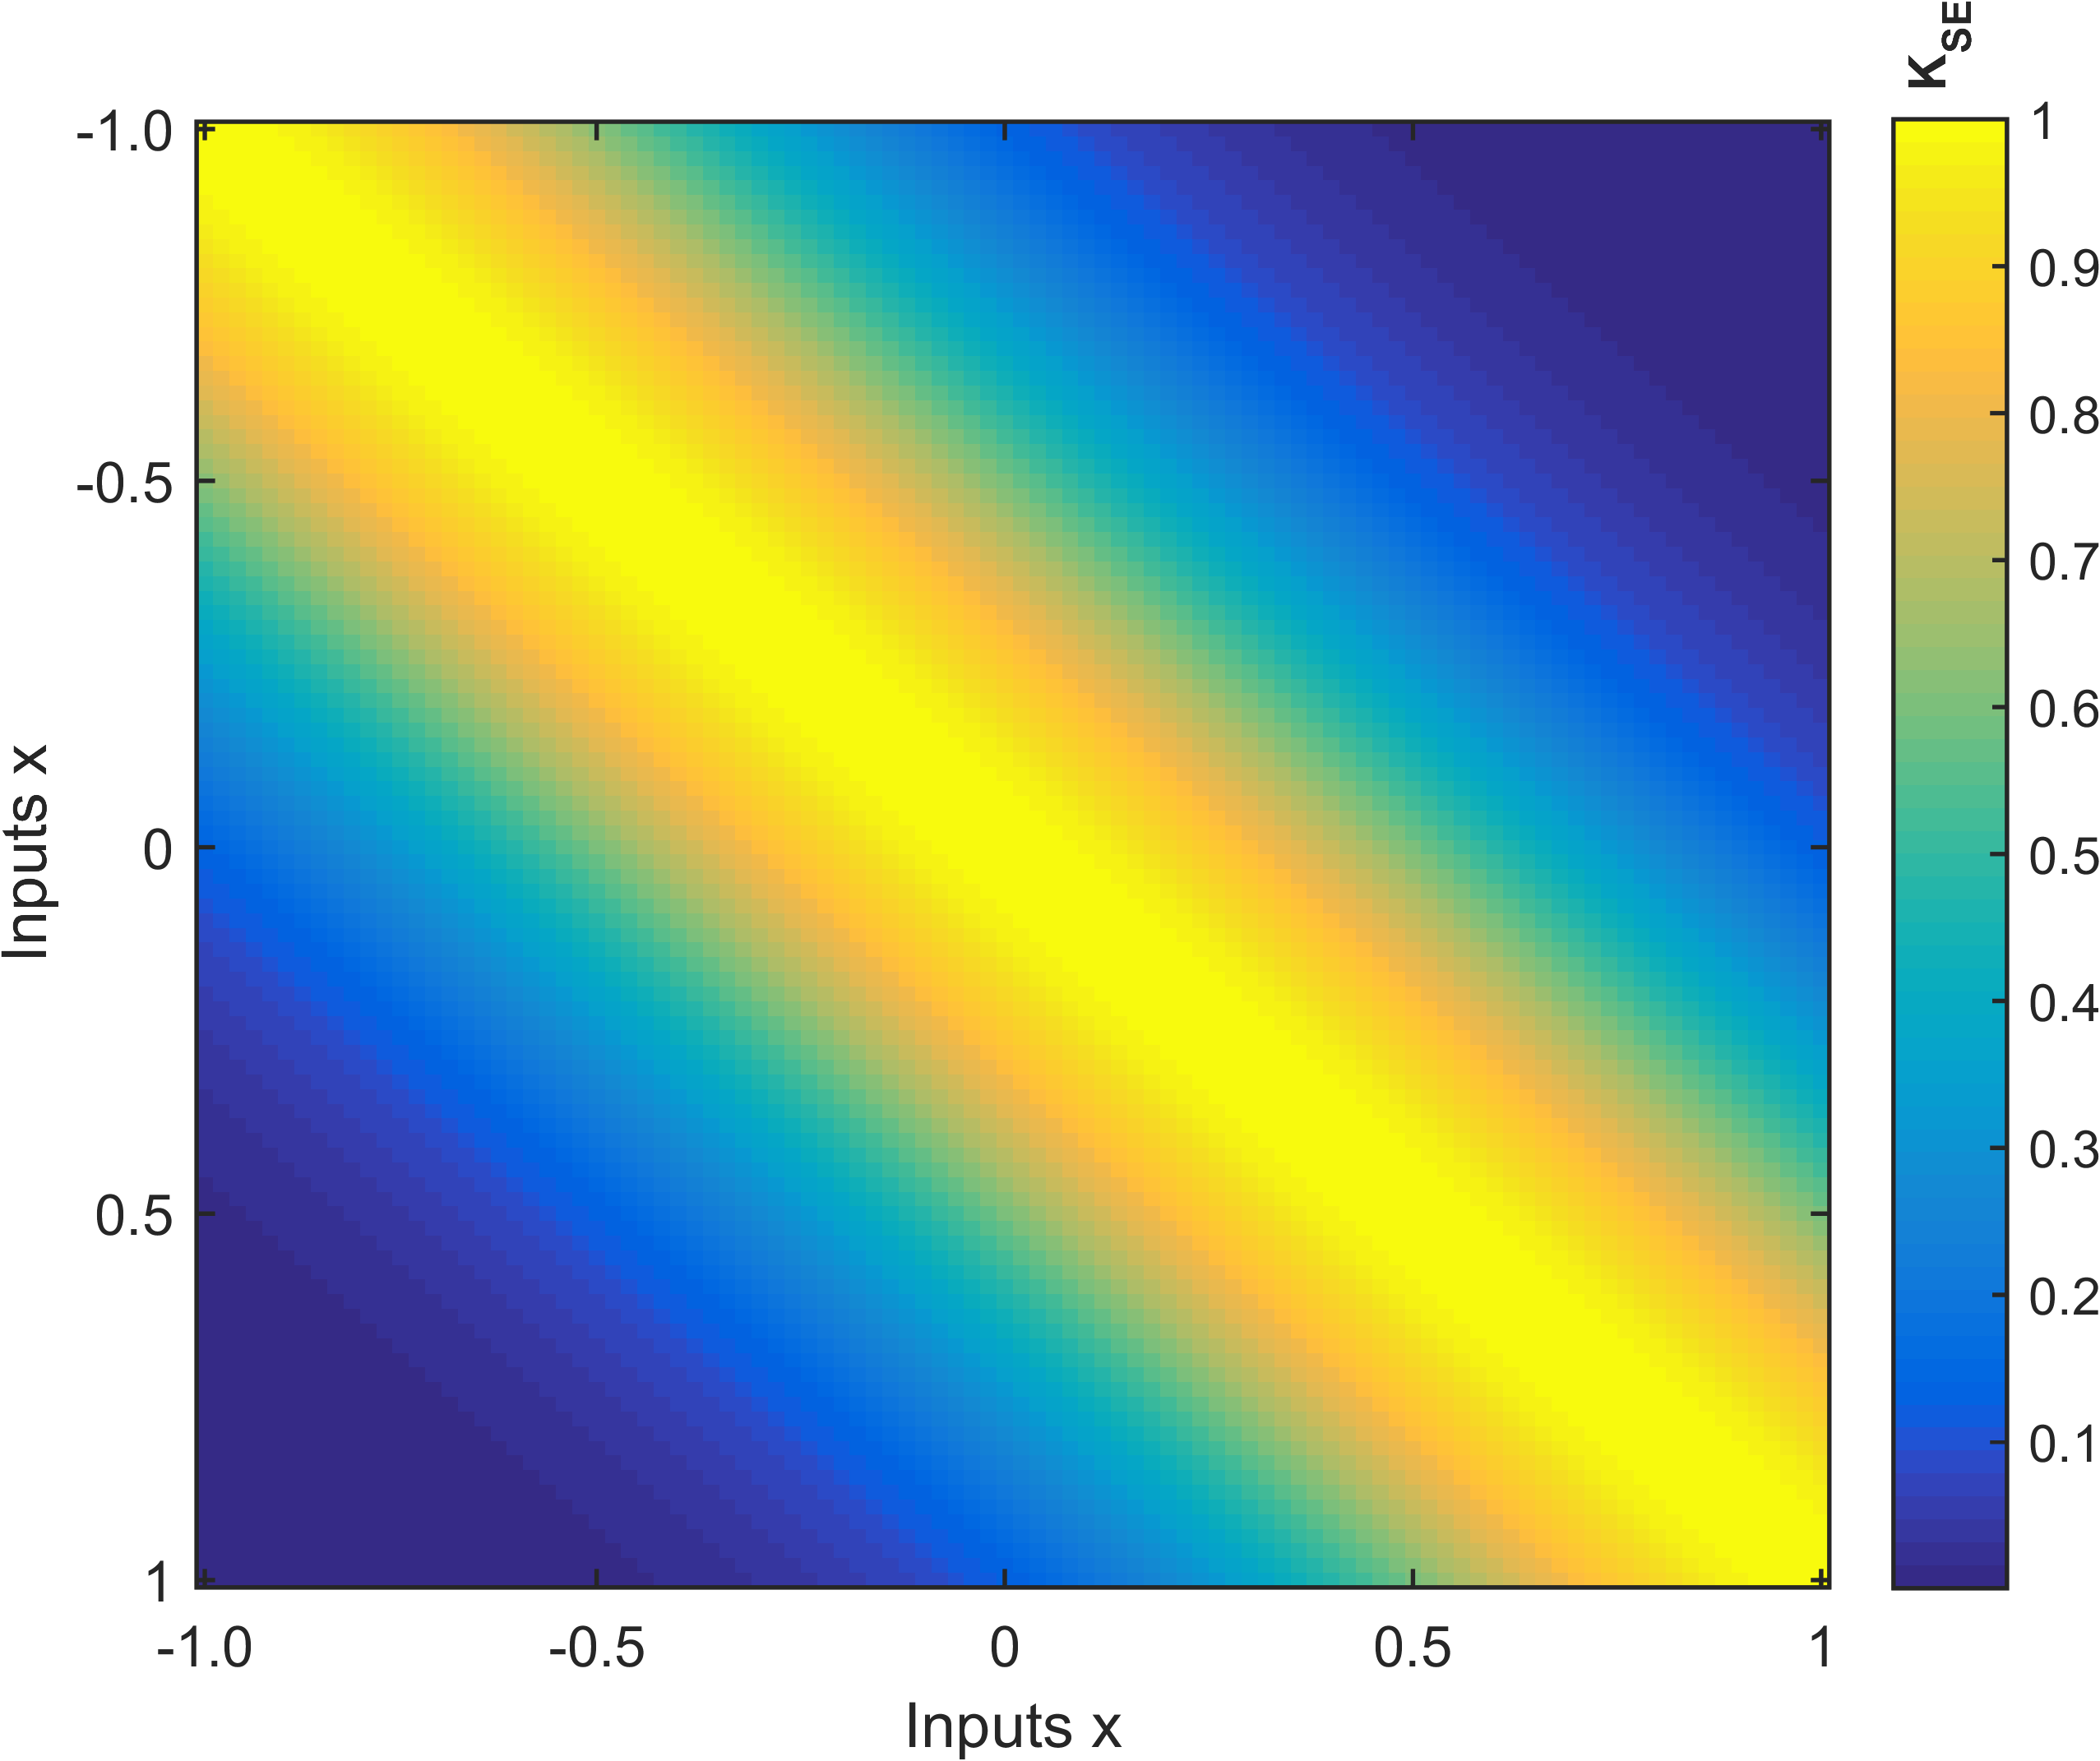
\includegraphics[width=0.45\textwidth]
        {images/covSEmatrix_2}
        \label{subFigcovSEmatrix_2}
  }\quad
  
       \caption{Covariance matrix for a Standard Exponential kernel with different hyper-parameters at the input points $X^{*} = \{[0:0.02:1]\}$. The SE kernel of figure \ref{subFigcovSEmatrix_1} has a lower length-scale than figure \ref{subFigcovSEmatrix_2}. Note, how the covariance values are more spread out for figure \ref{subFigcovSEmatrix_2}.}\label{figGPCovarianceMatrix}
\end{figure}

To generate a random Gaussian vector $f(X_{*})$ of length $N_{*}$, we first calculate the Cholesky decomposition\footnote{Cholesky Decomposition is also called the square-root of matrix and is defined for positive definite matrices} of the covariance matrix $K(X_{*}, X_{*}) = LL^{T}$, where $L$ is a lower triangular matrix. We then generate a random vector $U$, such that $U = \mathcal{N}(0, I)$ and $I$ is an identity matrix of size $N_{*}$.  The random vector can be then computed as, $f(X_{*}) = m(X_{*}) + LU$ and when plotted with the inputs $X_{*}$ gives a randomly drawn function. Figure \ref{figGPPriors} shows 5 random functions drawn for a zero mean GP with the covariance matrices of figure \ref{figGPCovarianceMatrix}. The solid black line defines the mean function, shaded blue region defines 95\% confidence interval (2$\sigma$) distance away from the mean. The dashed lines are five functions drawn at random from a GP prior. We can observe that figure \ref{subFigSEPrior_1} varies faster when compared to figure \ref{subFigSEPrior_2} due to smaller length scale hyper-parameter. 

\begin{figure}[!ht]
  \centering
    \subfigure[{Draws from a GP prior with mean zero and Standard Exponential (SE) Kernel with $(\theta = [1, 0.2])$. }]
  {
        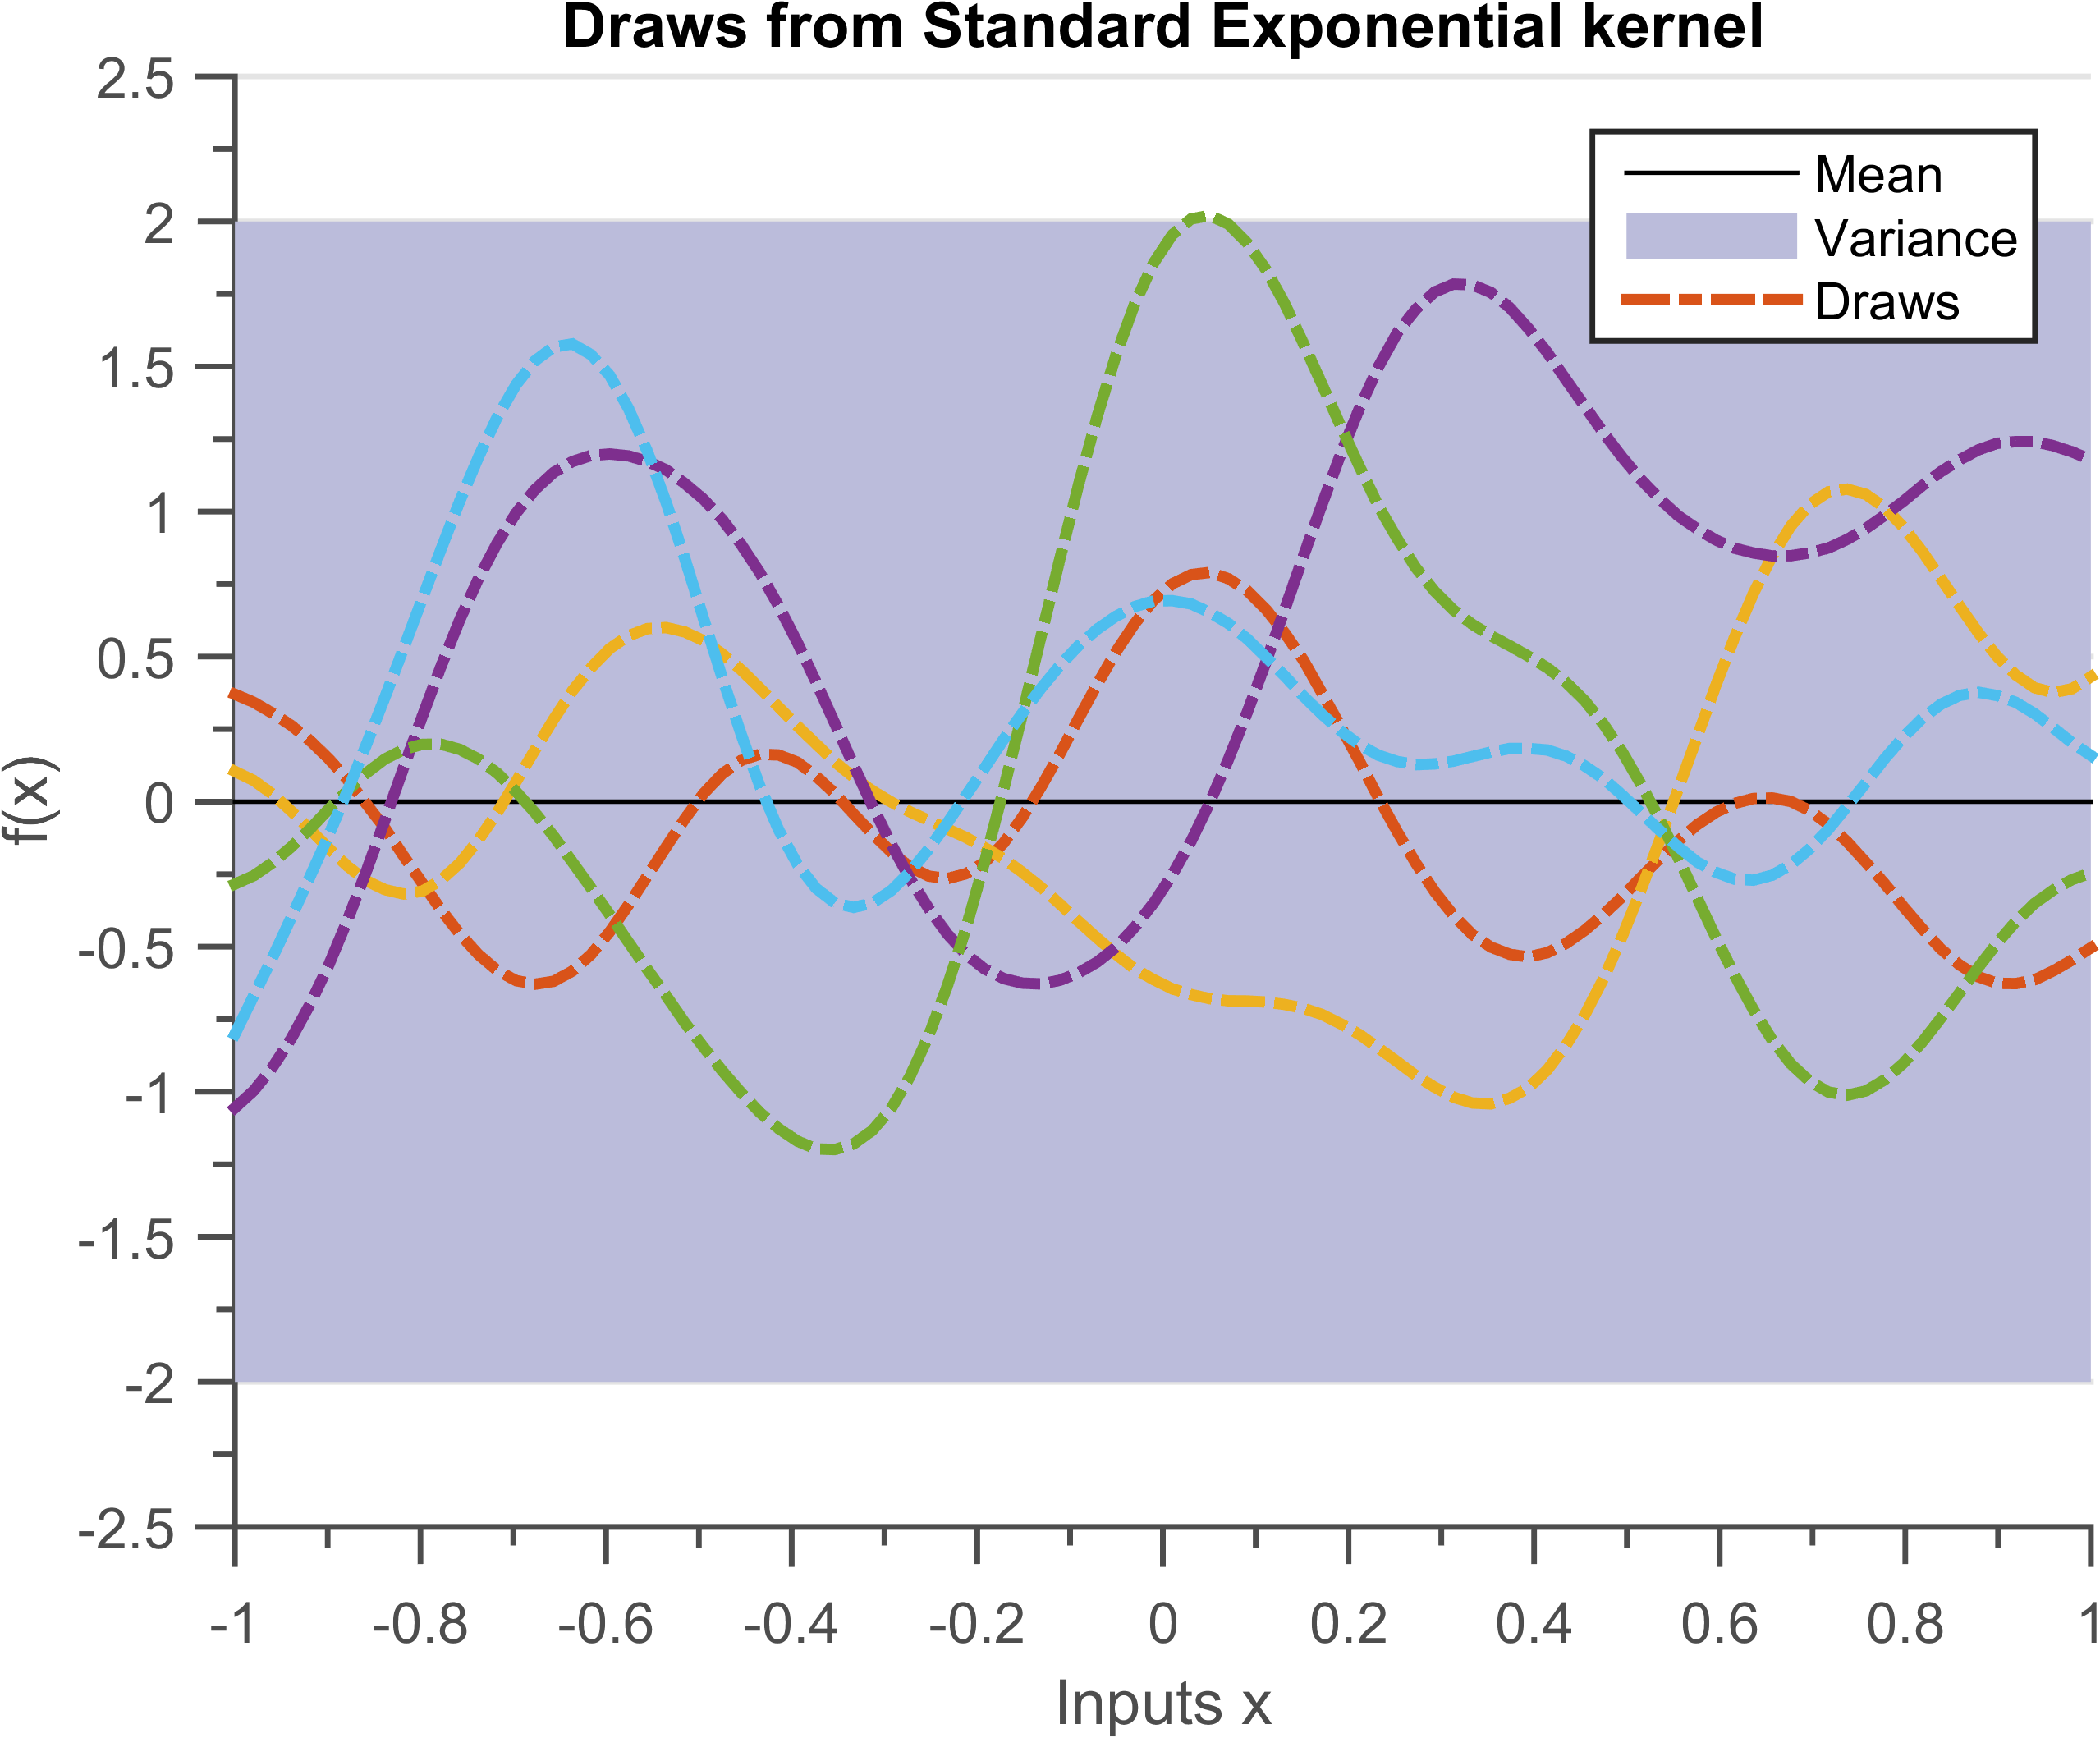
\includegraphics[width=0.45\textwidth]
        {images/drawsSEKernel_1}
        \label{subFigSEPrior_1}
  }\quad
\subfigure[{Draws from a GP prior with mean zero and Standard Exponential (SE) with $(\theta = [1, 0.5])$}]
  {
        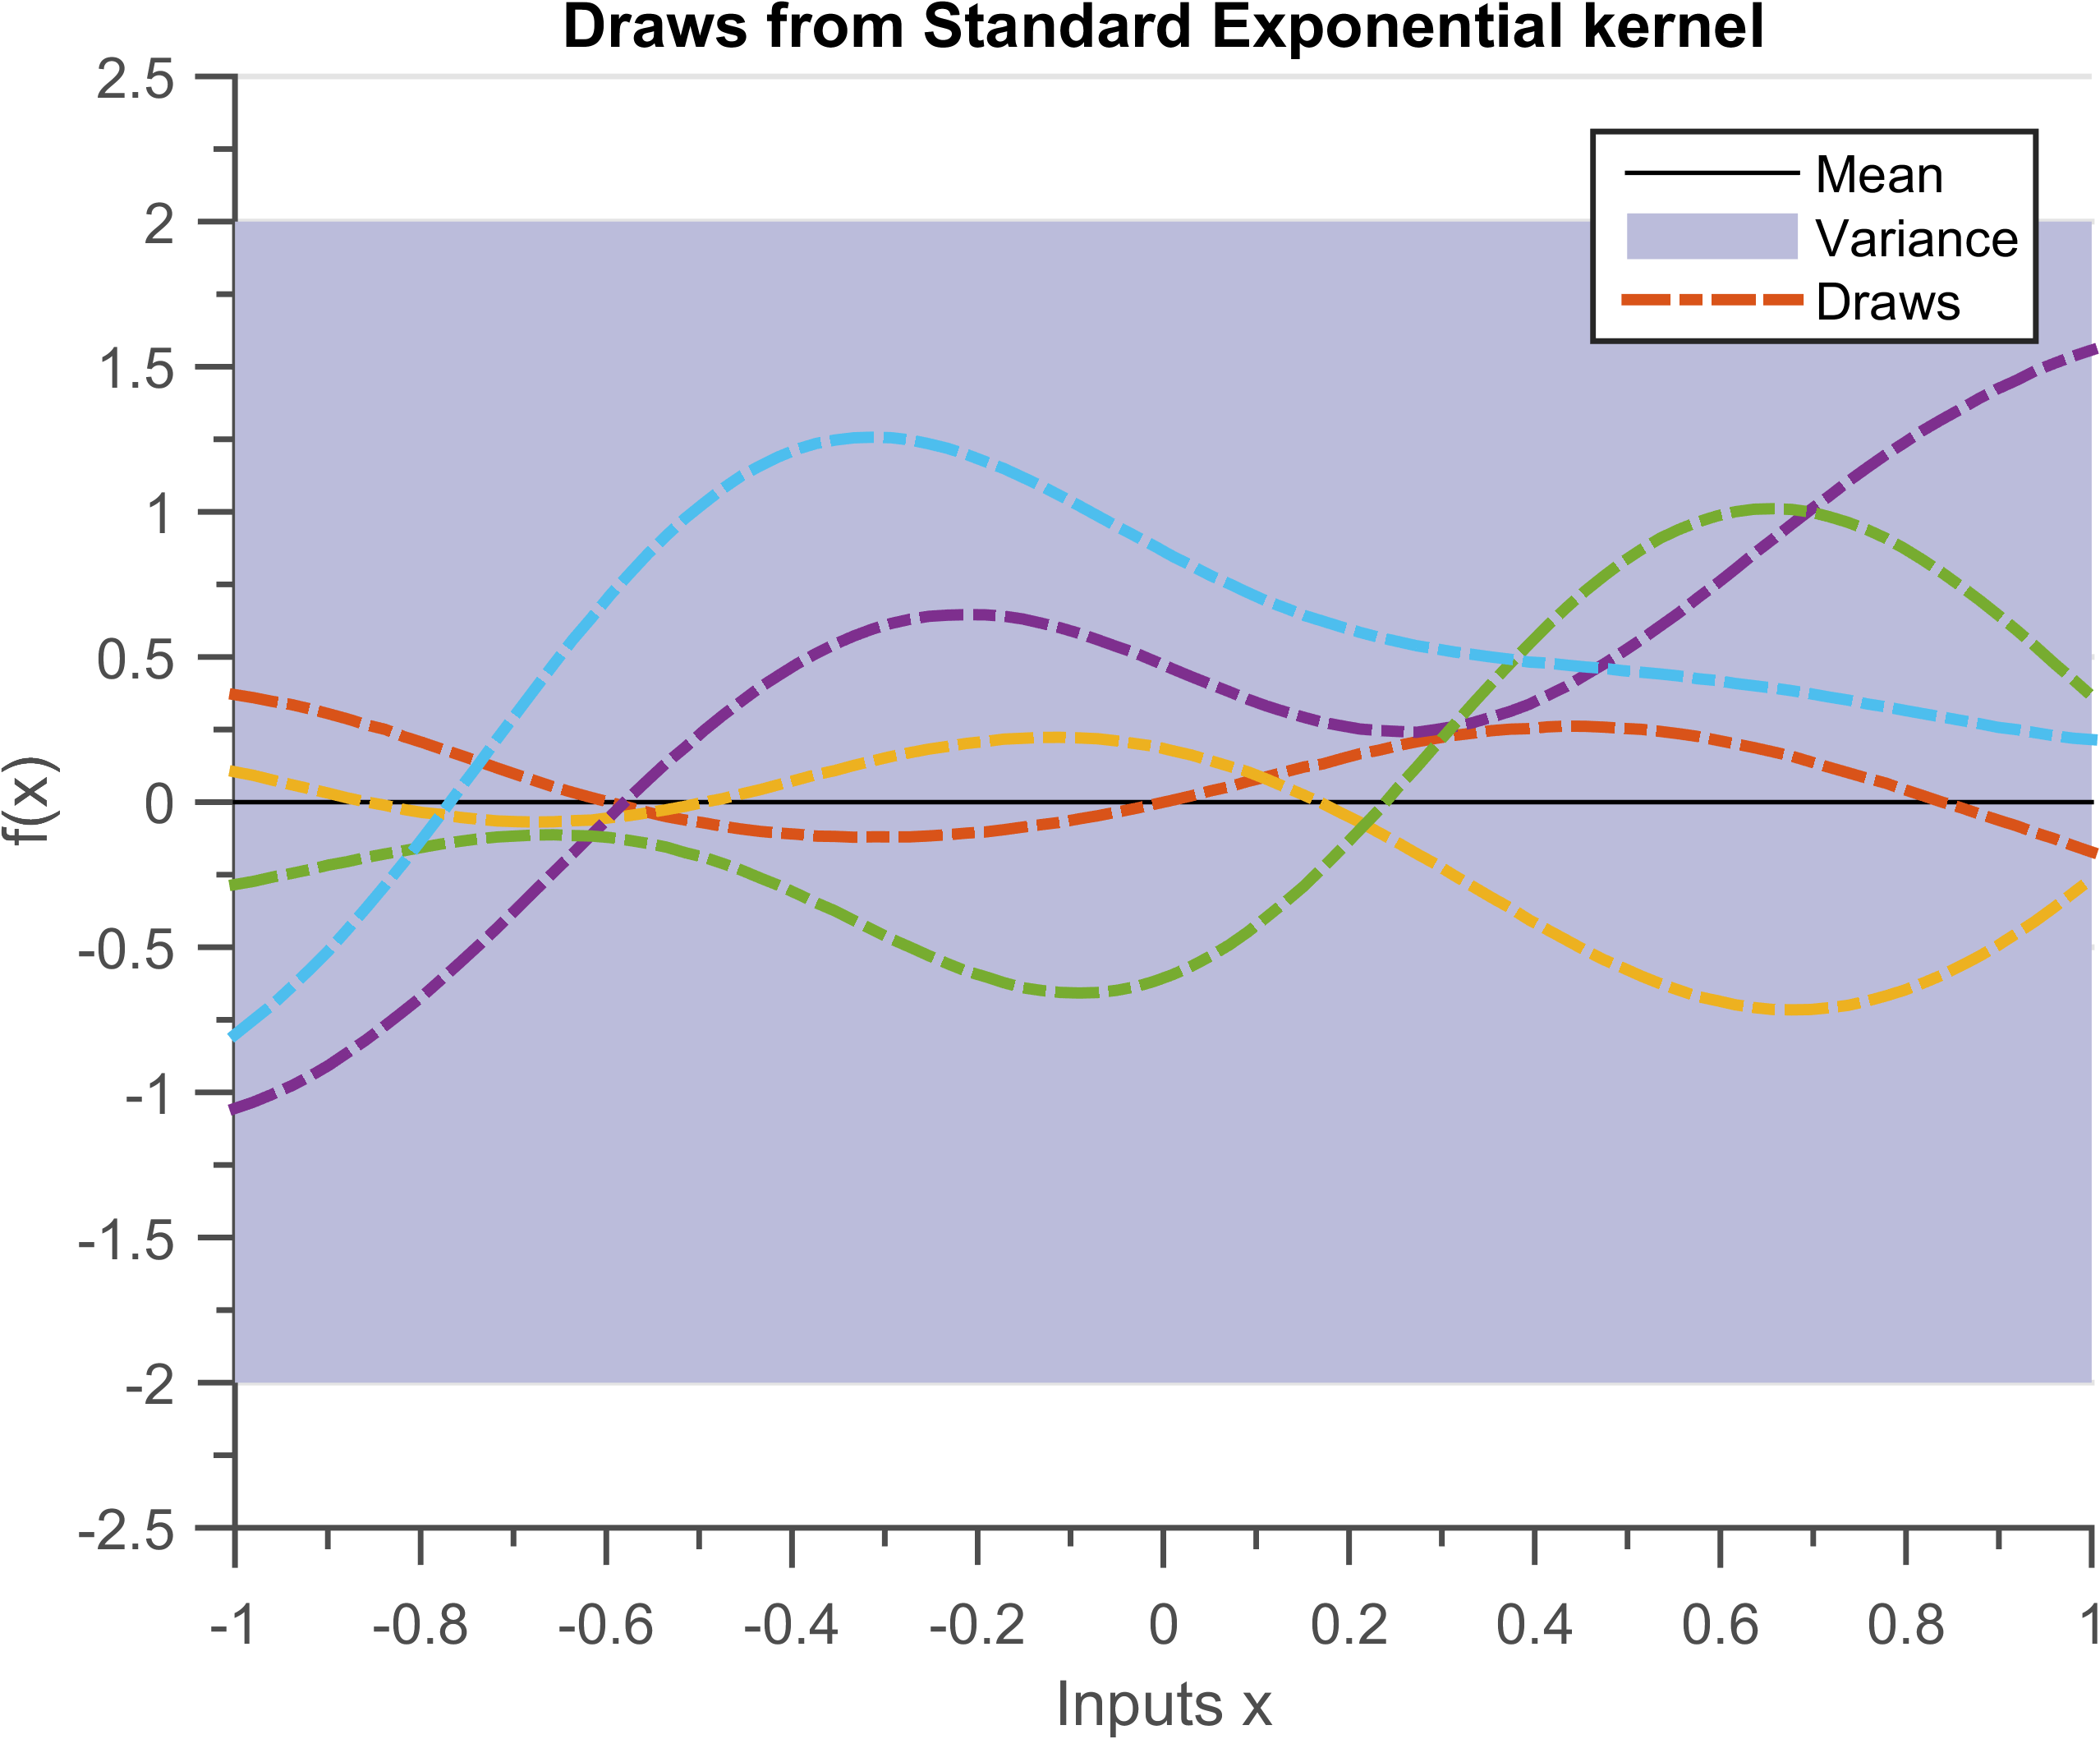
\includegraphics[width=0.45\textwidth]
        {images/drawsSEKernel_2}
        \label{subFigSEPrior_2}
  }\quad
  
       \caption{The solid black line defines the mean function, shaded blue region defines 95\% confidence interval (2$\sigma$) distance away from the mean. The dashed lines are five functions drawn at random from a GP prior. We can observe that figure \ref{subFigSEPrior_1} varies faster when compared to figure \ref{subFigSEPrior_2} due to smaller length scale hyper-parameter.       }\label{figGPPriors}
\end{figure}



\section{Posterior}\label{secPosterior}
Once we have defined an appropriate prior we wish to incorporate the information of training data set into the probabilistic framework. In the Bayesian framework, a posterior is the probability distribution after updating the information of evidence into prior knowledge. 


\subsection{Posterior with Noise-free observations}\label{subSecPosteriorNoiseFree}
We first consider the case of noise-free observations, that is we know $\{y(x_{i}) = f_{i} | i \in [1; N] \}$. This is case for many high-fidelity computer simulations, since high-fidelity computer simulations can be treated as having no noise \cite{sacks1989design}. If we desire to interpolate at $N_{*}$ test points $X_{*}$, then the multi-variate distribution of the training outputs $f(X)$ and test outputs $f(X_{*})$ according to the GP prior, test and training points is given by equation \ref{equationJointPriorNoiseFree}.

\begin{equation}\label{equationJointPriorNoiseFree}
\Pr\left [ \begin{matrix}
f(X)
\\ f(X_{*})
\end{matrix} \right ] = 
\mathcal{N}\left (\left [ \begin{matrix} 0 \\ 0 \end{matrix} \right ]
, 
\left [ \begin{matrix}
K(X, X) & K(X, X_{*})\\ 
K(X_{*}, X) & K(X_{*}, X_{*})
\end{matrix} \right ]
\right)
\end{equation}

$K(X, X_{*})$ is $N \times N_{*}$ covariance matrix between the training points $X$ and test points $X_{*}$ (equation \ref{eqnCovMatrixSquaredExponential}). The other covariance matrices $K(X, X)$, $K(X_{*}, X)$ and $K(X_{*}, X_{*})$ can be computed similarly. 

The posterior will be the the conditional probability of $f(X_{*})$ given the prior and data set. For a multi-variate Gaussian the conditional distribution is also a multi-variate Gaussian and can be calculated tractably, for a more detailed derivation refer to appendix \textbf{refer to the appendix here}. Graphically, we can imagine that the Bayes theorem is removing all the functions from our prior family of functions that do not pass through the data set (figure \ref{figGPNoiseLessPosteriors}). The predicted distribution after adding the information of data set into the prior can be written as:

  \begin{equation}\label{eqNoiseFreePosteriorGP}
  \begin{aligned}
  \Pr(f(X_{*}) \mid X_{*}, X, f(X)) = GP(  & K(X_{*}, X)( K(X, X) )^{-1}f(X),   \\ 
                                & K(X_{*}, X_{*}) - K(X_{*}, X)( K(X, X) )^{-1} K(X, X_{*}))
  \end{aligned}
  \end{equation}

The term $K(X_{*}, X)( K(X, X) )^{-1}f(X)$ is the predicted mean of the posterior at the test points $X_{*}$. The term $K(X_{*}, X_{*}) - K(X_{*}, X)( K(X, X) )^{-1} K(X, X_{*})$ is the predicted covariance. 

\textbf{define $\mathcal{D}_{2}$}


\begin{figure}[!ht]
  \centering
    \subfigure[{Posterior distribution for the case of noiseless observations. Prior is a GP with mean zero and covariance as Standard Exponential (SE) Kernel with $(\theta = [1, 0.2])$, data set is $\{x = -0.5; f = 0\}$.}]
  {
        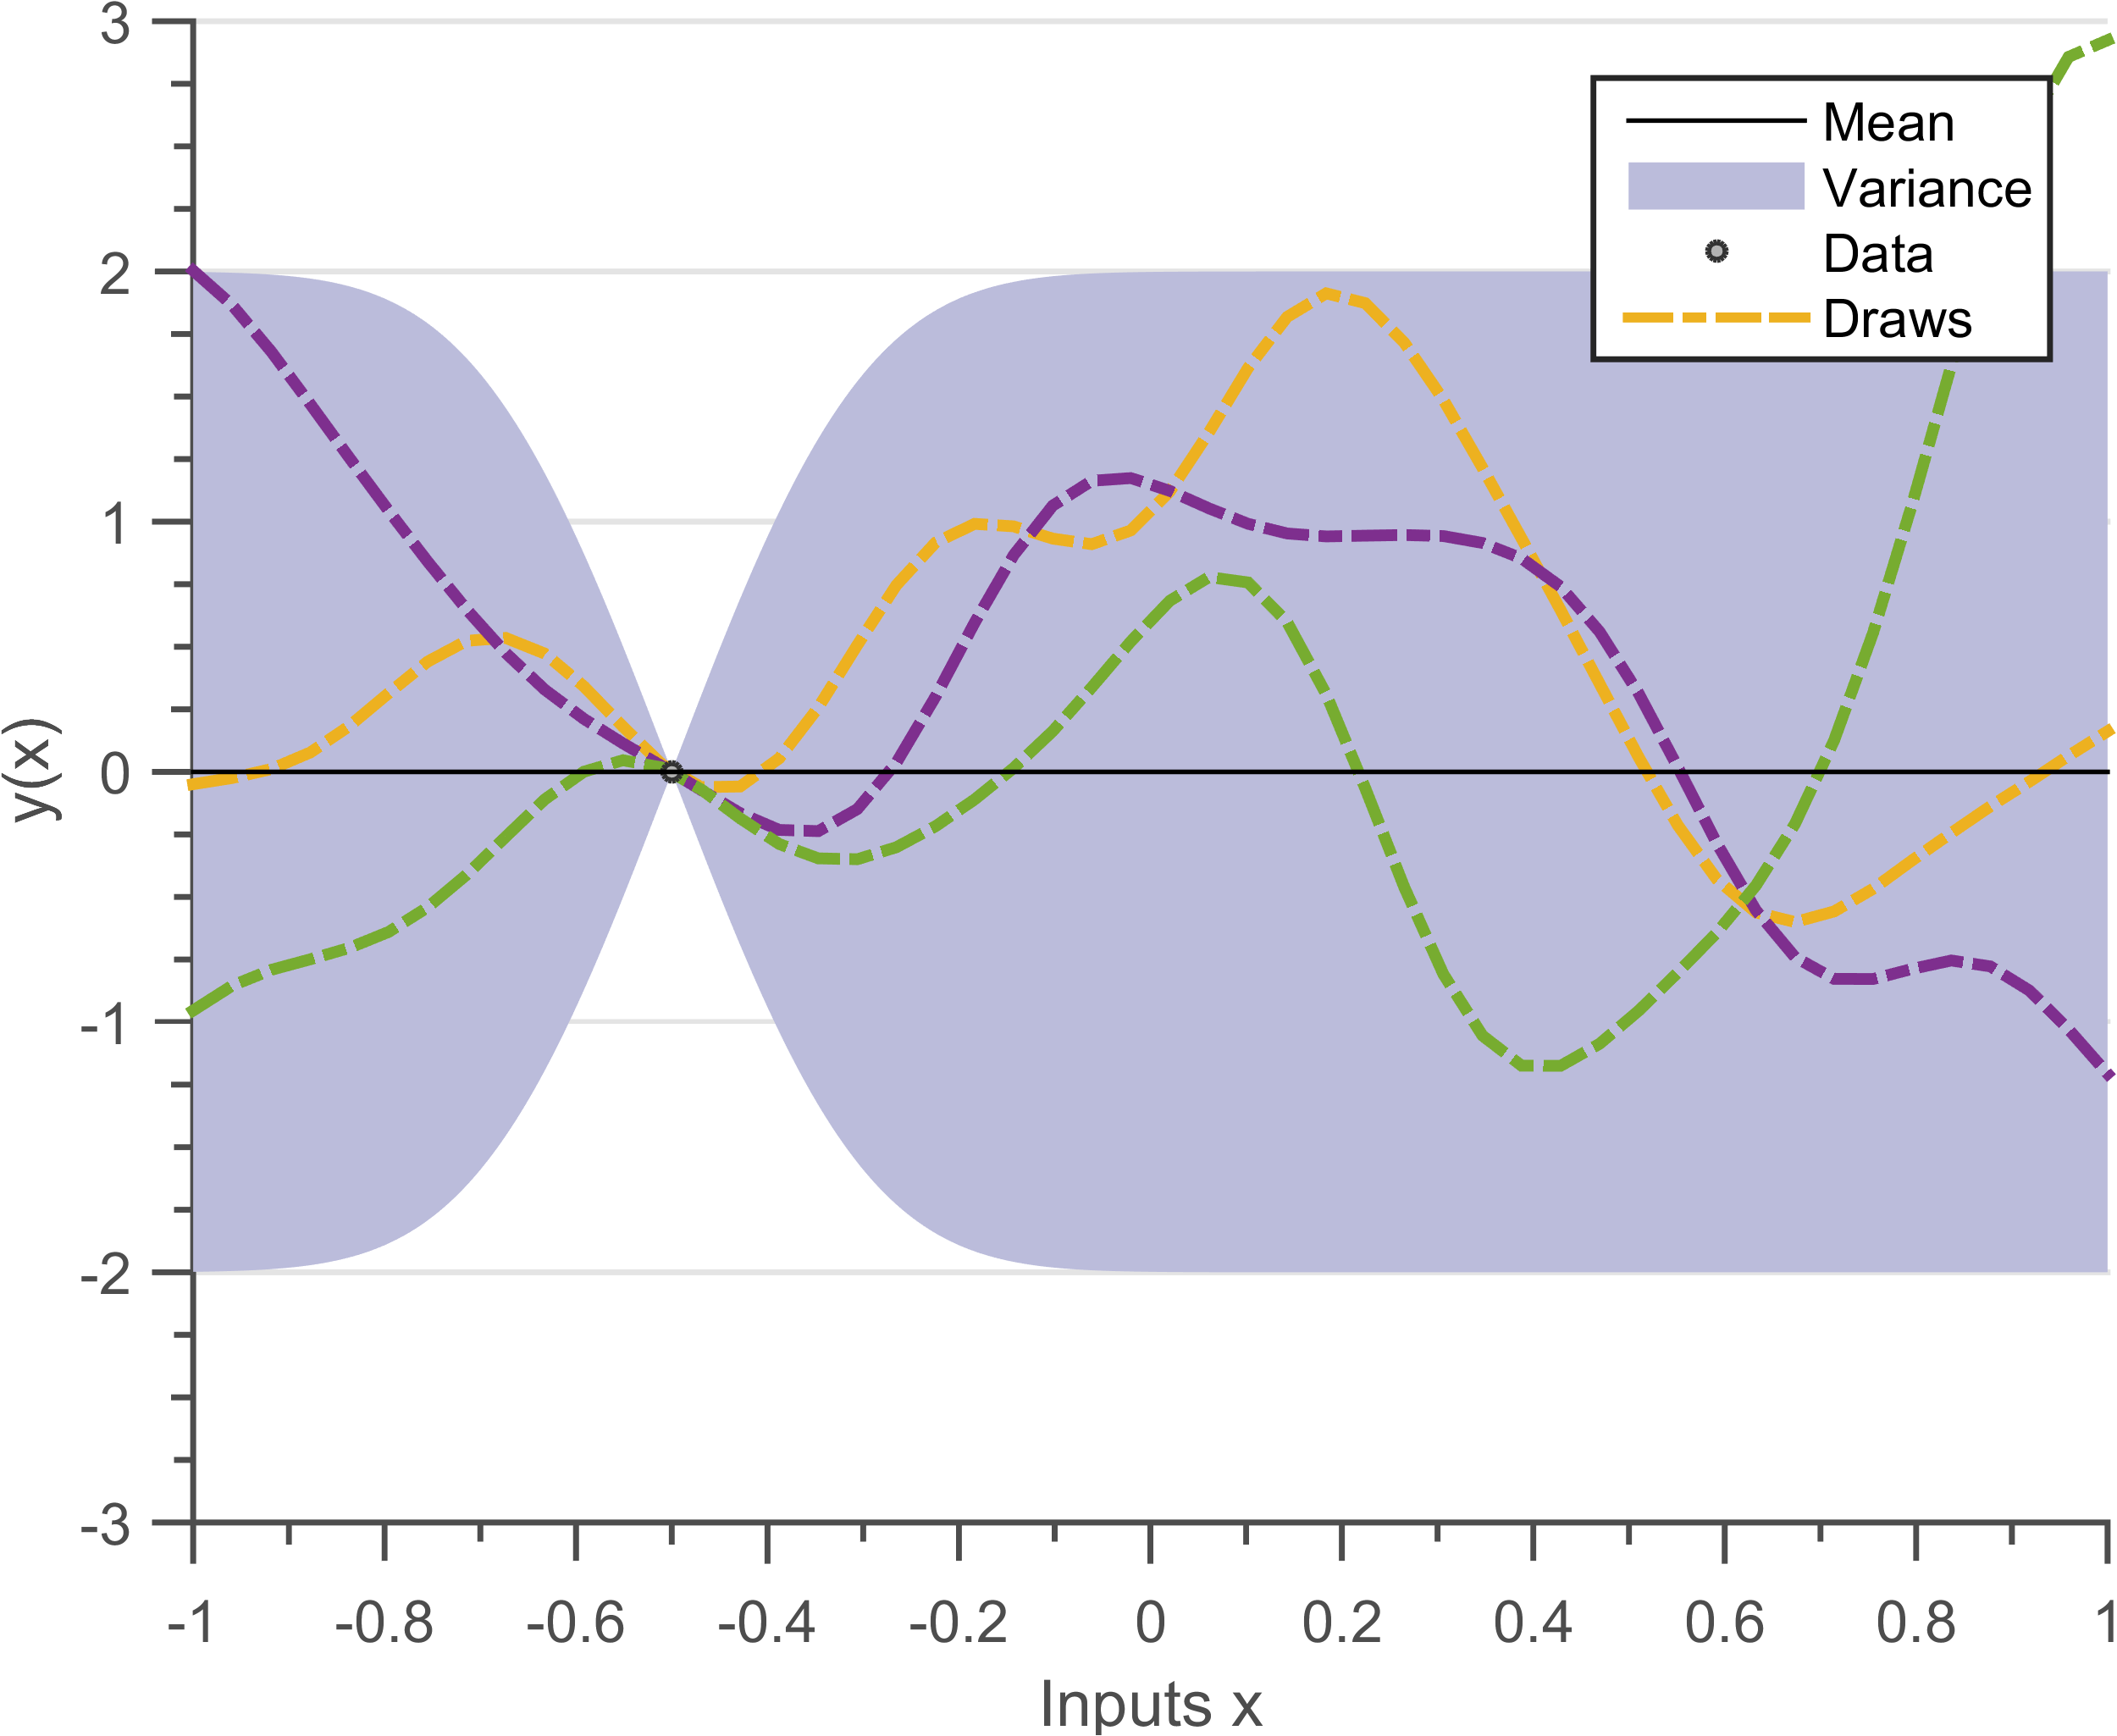
\includegraphics[width=0.45\textwidth]
        {images/posteriorSENoiseLess_1}
        \label{posteriorSENoiseLess_1}
  }\quad
\subfigure[{Posterior distribution for the case of noiseless observations. Prior is a GP with mean zero and covariance as Standard Exponential (SE) Kernel with $(\theta = [1, 0.2])$, data set is $\{x = [-0.5, 0.33, 0.66]; f = [0, 0.5, 0.5]\}$}.  ]
  {
        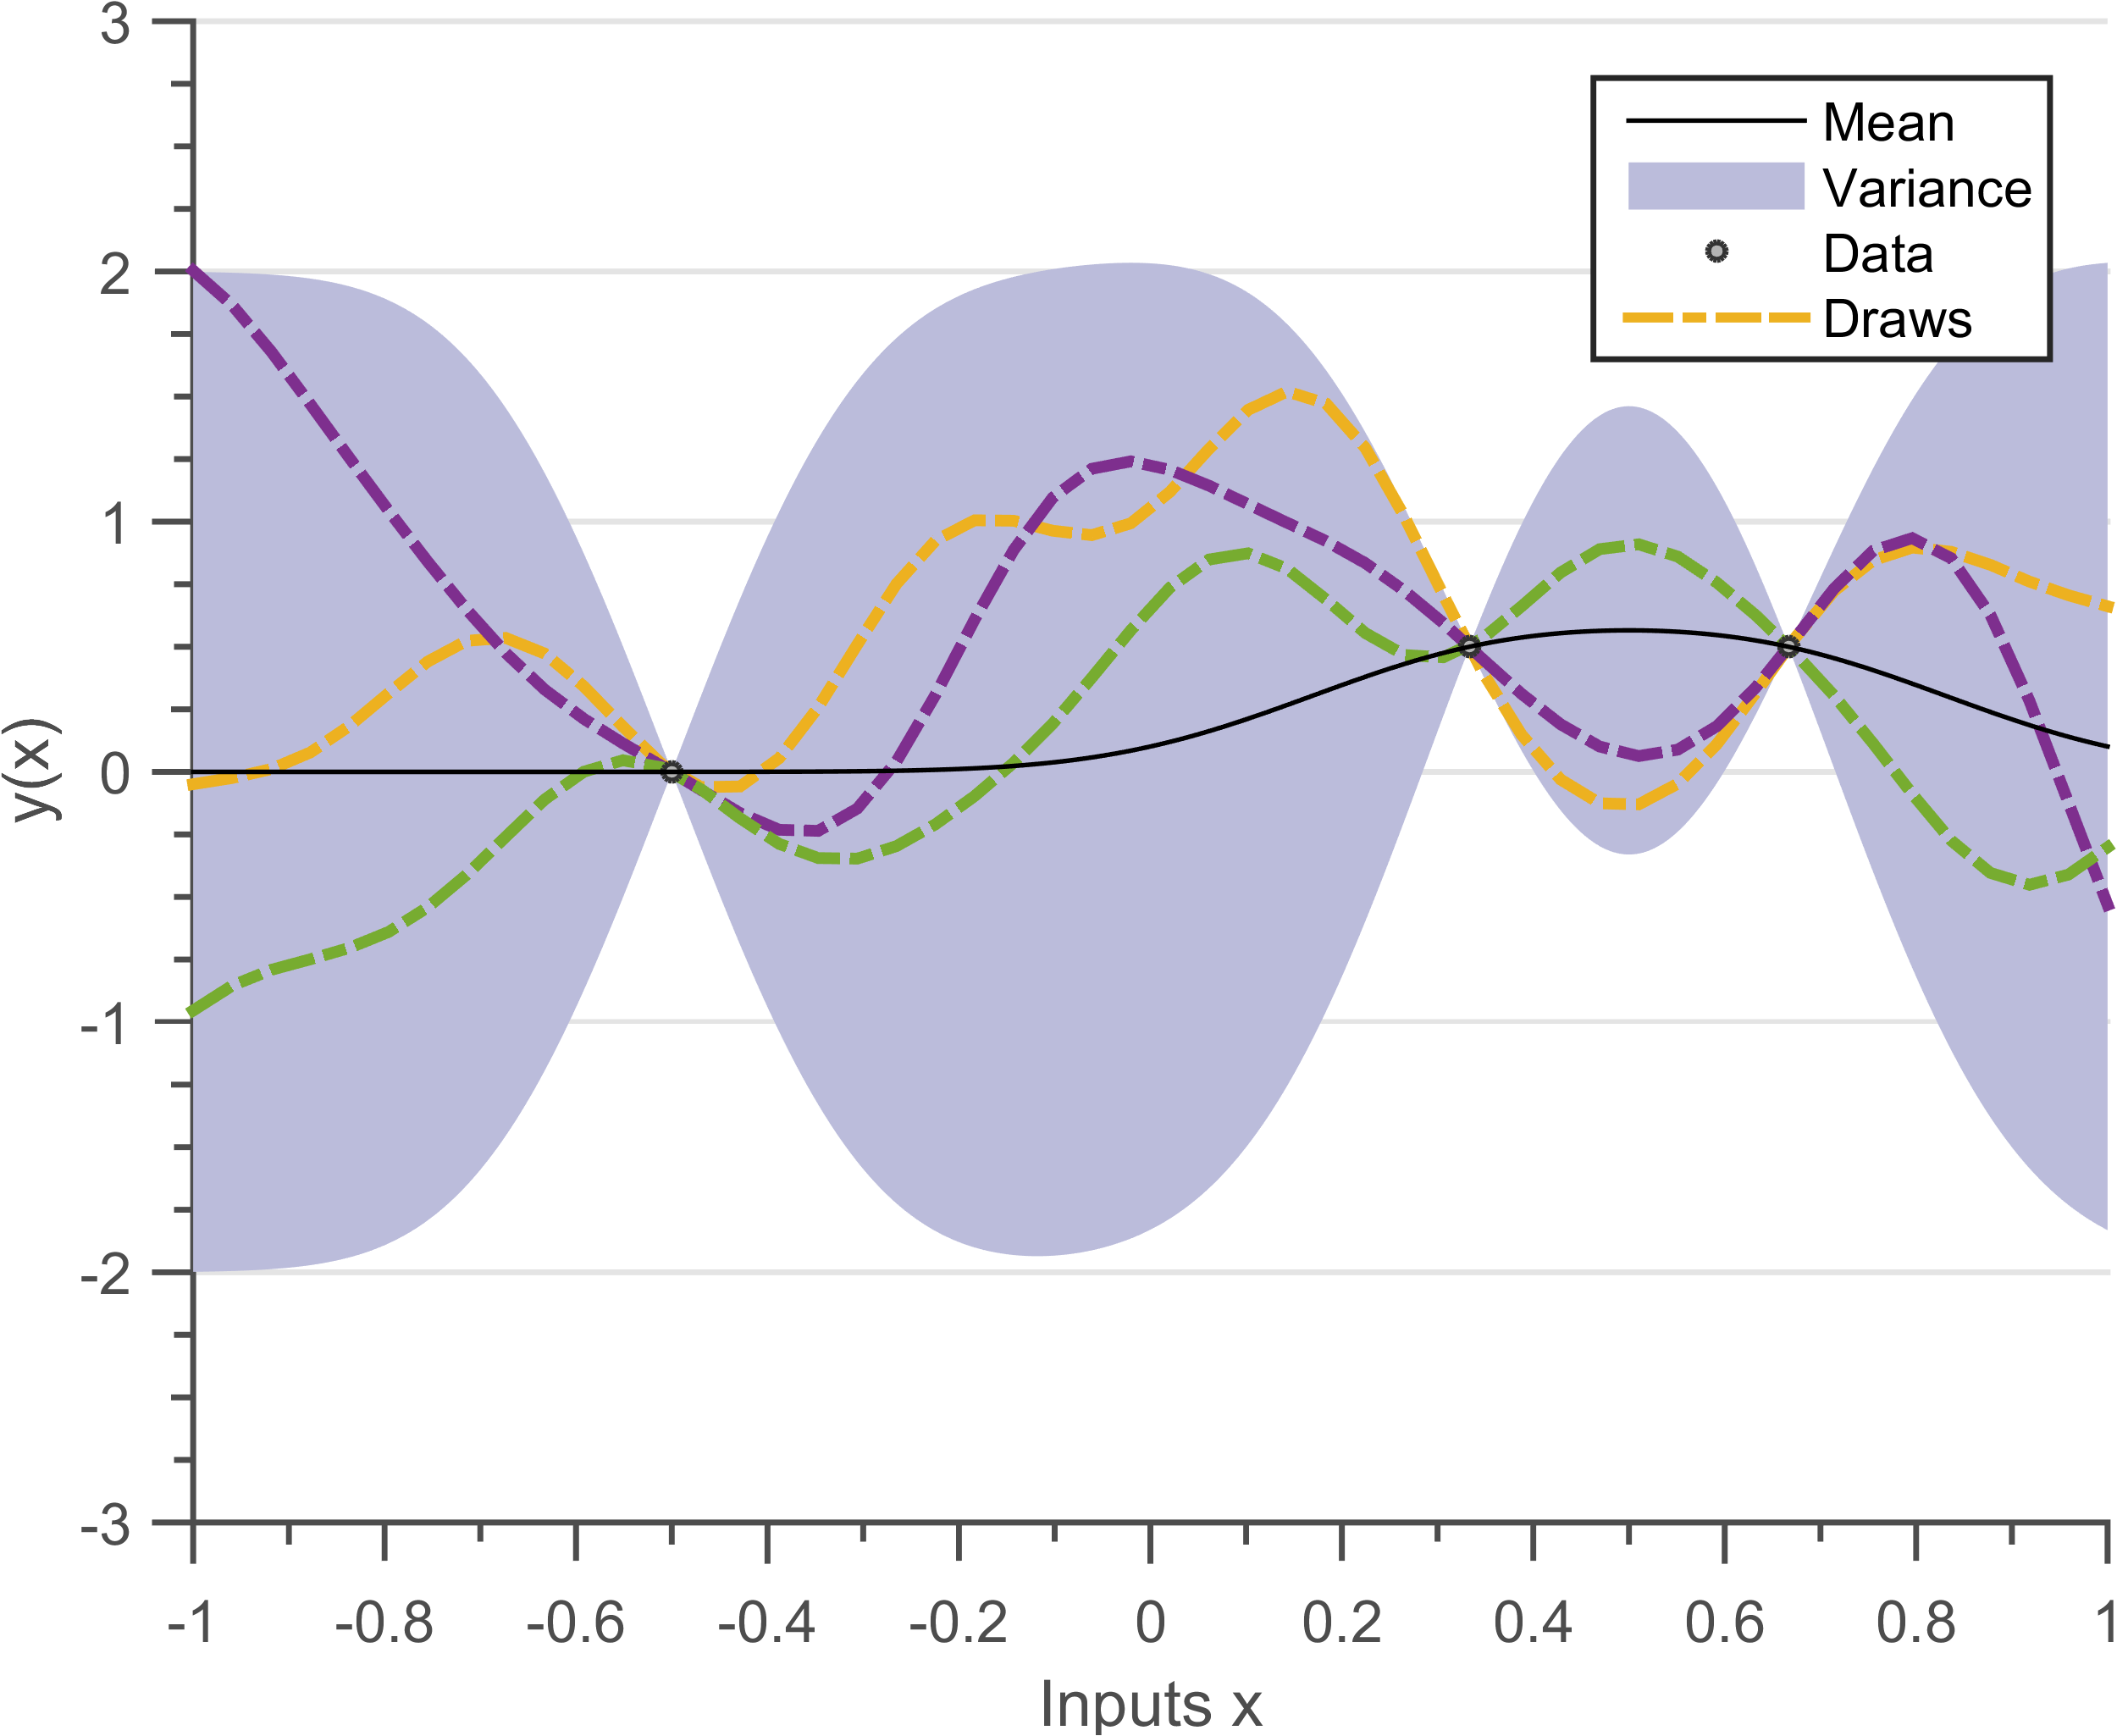
\includegraphics[width=0.45\textwidth]
        {images/posteriorSENoiseLess_3}
        \label{posteriorSENoiseLess_3}
  }\quad
  
       \caption{Prediction in the case of noiseless observations. The solid black line defines the mean function, blue region defines 95\% confidence interval (2$\sigma$) distance away from the mean. The dashed lines are three functions drawn at random from a GP posterior. We can observe that Bayes Theorem eliminates all the functions that do not pass through the observed data-set.}
       \label{figGPNoiseLessPosteriors}
\end{figure}

Figure \ref{figGPNoiseLessPosteriors} shows the posterior GP after adding observed data into the initial prior. We can see that Bayes theorem eliminates all the functions in the prior that does not pass through the data. The solid black line defines the mean function, blue region defines 95\% confidence interval (2$\sigma$) distance away from the mean. The mean of the of the posterior distribution is also used as a point estimate for interpolation. The dashed lines are three functions drawn at random from a GP posterior. Random functions can be sampled from the posterior distribution as described in the earlier section. 

\subsection{Posterior with Noisy observations}\label{subSecPosteriorNoisy}
If we assume a more general case of noisy observations then the measured outputs can be written as:

\begin{equation}\label{eqNoiseEquation}
y(x) = f(x) + \epsilon
\end{equation}

Such that $\epsilon$ is an independent random noise sampled from a white noise Gaussian $\mathcal{N}(0, \sigma_{n}^{2})$. We can thus write the prior GP of the noisy case as:

\begin{equation}\label{equationMeanZeroGPNoisydefinition}
\Pr[y(x) \mid X, \sigma_{n}] = GP(0 , k(x_{1}, x_{2}) + \sigma^{2}_{n}\delta_{xx'})
\end{equation}

Here, $\delta_{xx'}$ is a Kronecker delta which is one iff $x = x'$ and zero otherwise. Since the noise is independent for each observation hence there is no noise term for covariances between inputs. The joint distribution of the training outputs $Y(X)$ and true physical process $f(X_{*})$ according to the above prior becomes:

\begin{equation}\label{equationJointPriorNoisy}
\Pr\left [ \begin{matrix}
Y(X)
\\ f(X_{*})
\end{matrix} \right ]
= 
\mathcal{N}\left (
\left [ \begin{matrix}
0
\\ 0

\end{matrix} \right ] , \left [ \begin{matrix}
K(X, X) + \sigma^{2}_{n}I & K(X, X_{*})\\ 
K(X_{*}, X) & K(X_{*}, X_{*})
\end{matrix} \right ] 
\right )
\end{equation}

The difference between equation \ref{equationJointPriorNoisy} and \ref{equationJointPriorNoiseFree} is the addition of noise term $\sigma^{2}_{n}I$. The noise is assumed to be independent hence is multiplied to an identity matrix, to know how to add more complex noise models please refer to chapter \ref{chapBasicCovarianceKernels}. The posterior distribution of $f(X_{*})$ can be calculated as:

  \begin{equation}\label{eqNoisyPredictiveGP}
  \begin{aligned}
      \Pr(f(X_{*}) \mid X_{*}, X, Y(X)) = GP(  & K(X_{*}, X)( K(X, X) + \sigma^{2}_{n}I)^{-1}f(X),   \\ 
                                & K(X_{*}, X_{*}) - K(X_{*}, X)( K(X, X) + \sigma^{2}_{n}I)^{-1} K(X, X_{*}) 
  \end{aligned}
  \end{equation}

Figure \ref{figGPNoisyPosteriors} shows the posterior GP after adding observed data into the initial prior. The solid black line defines the mean function, blue region defines 95\% confidence interval (2$\sigma$) distance away from the mean. The dashed lines are three functions drawn at random from a GP posterior. Random functions can be sampled from the posterior distribution as described in the earlier section \ref{secPrior}.  Due to the inclusion of noise in the prior, we see that the draws from posterior are not necessarily passing from the observed point.

\begin{figure}[!ht]
  \centering
    \subfigure[{Posterior distribution for the case of noisy observations. Prior is a GP with mean zero, covariance as Standard Exponential (SE) Kernel with $(\theta = [1, 0.2])$ and noise as $\sigma_{n} = [0.02])$, , data set is $\{x = -0.5; f = 0\}$.}]
  {
        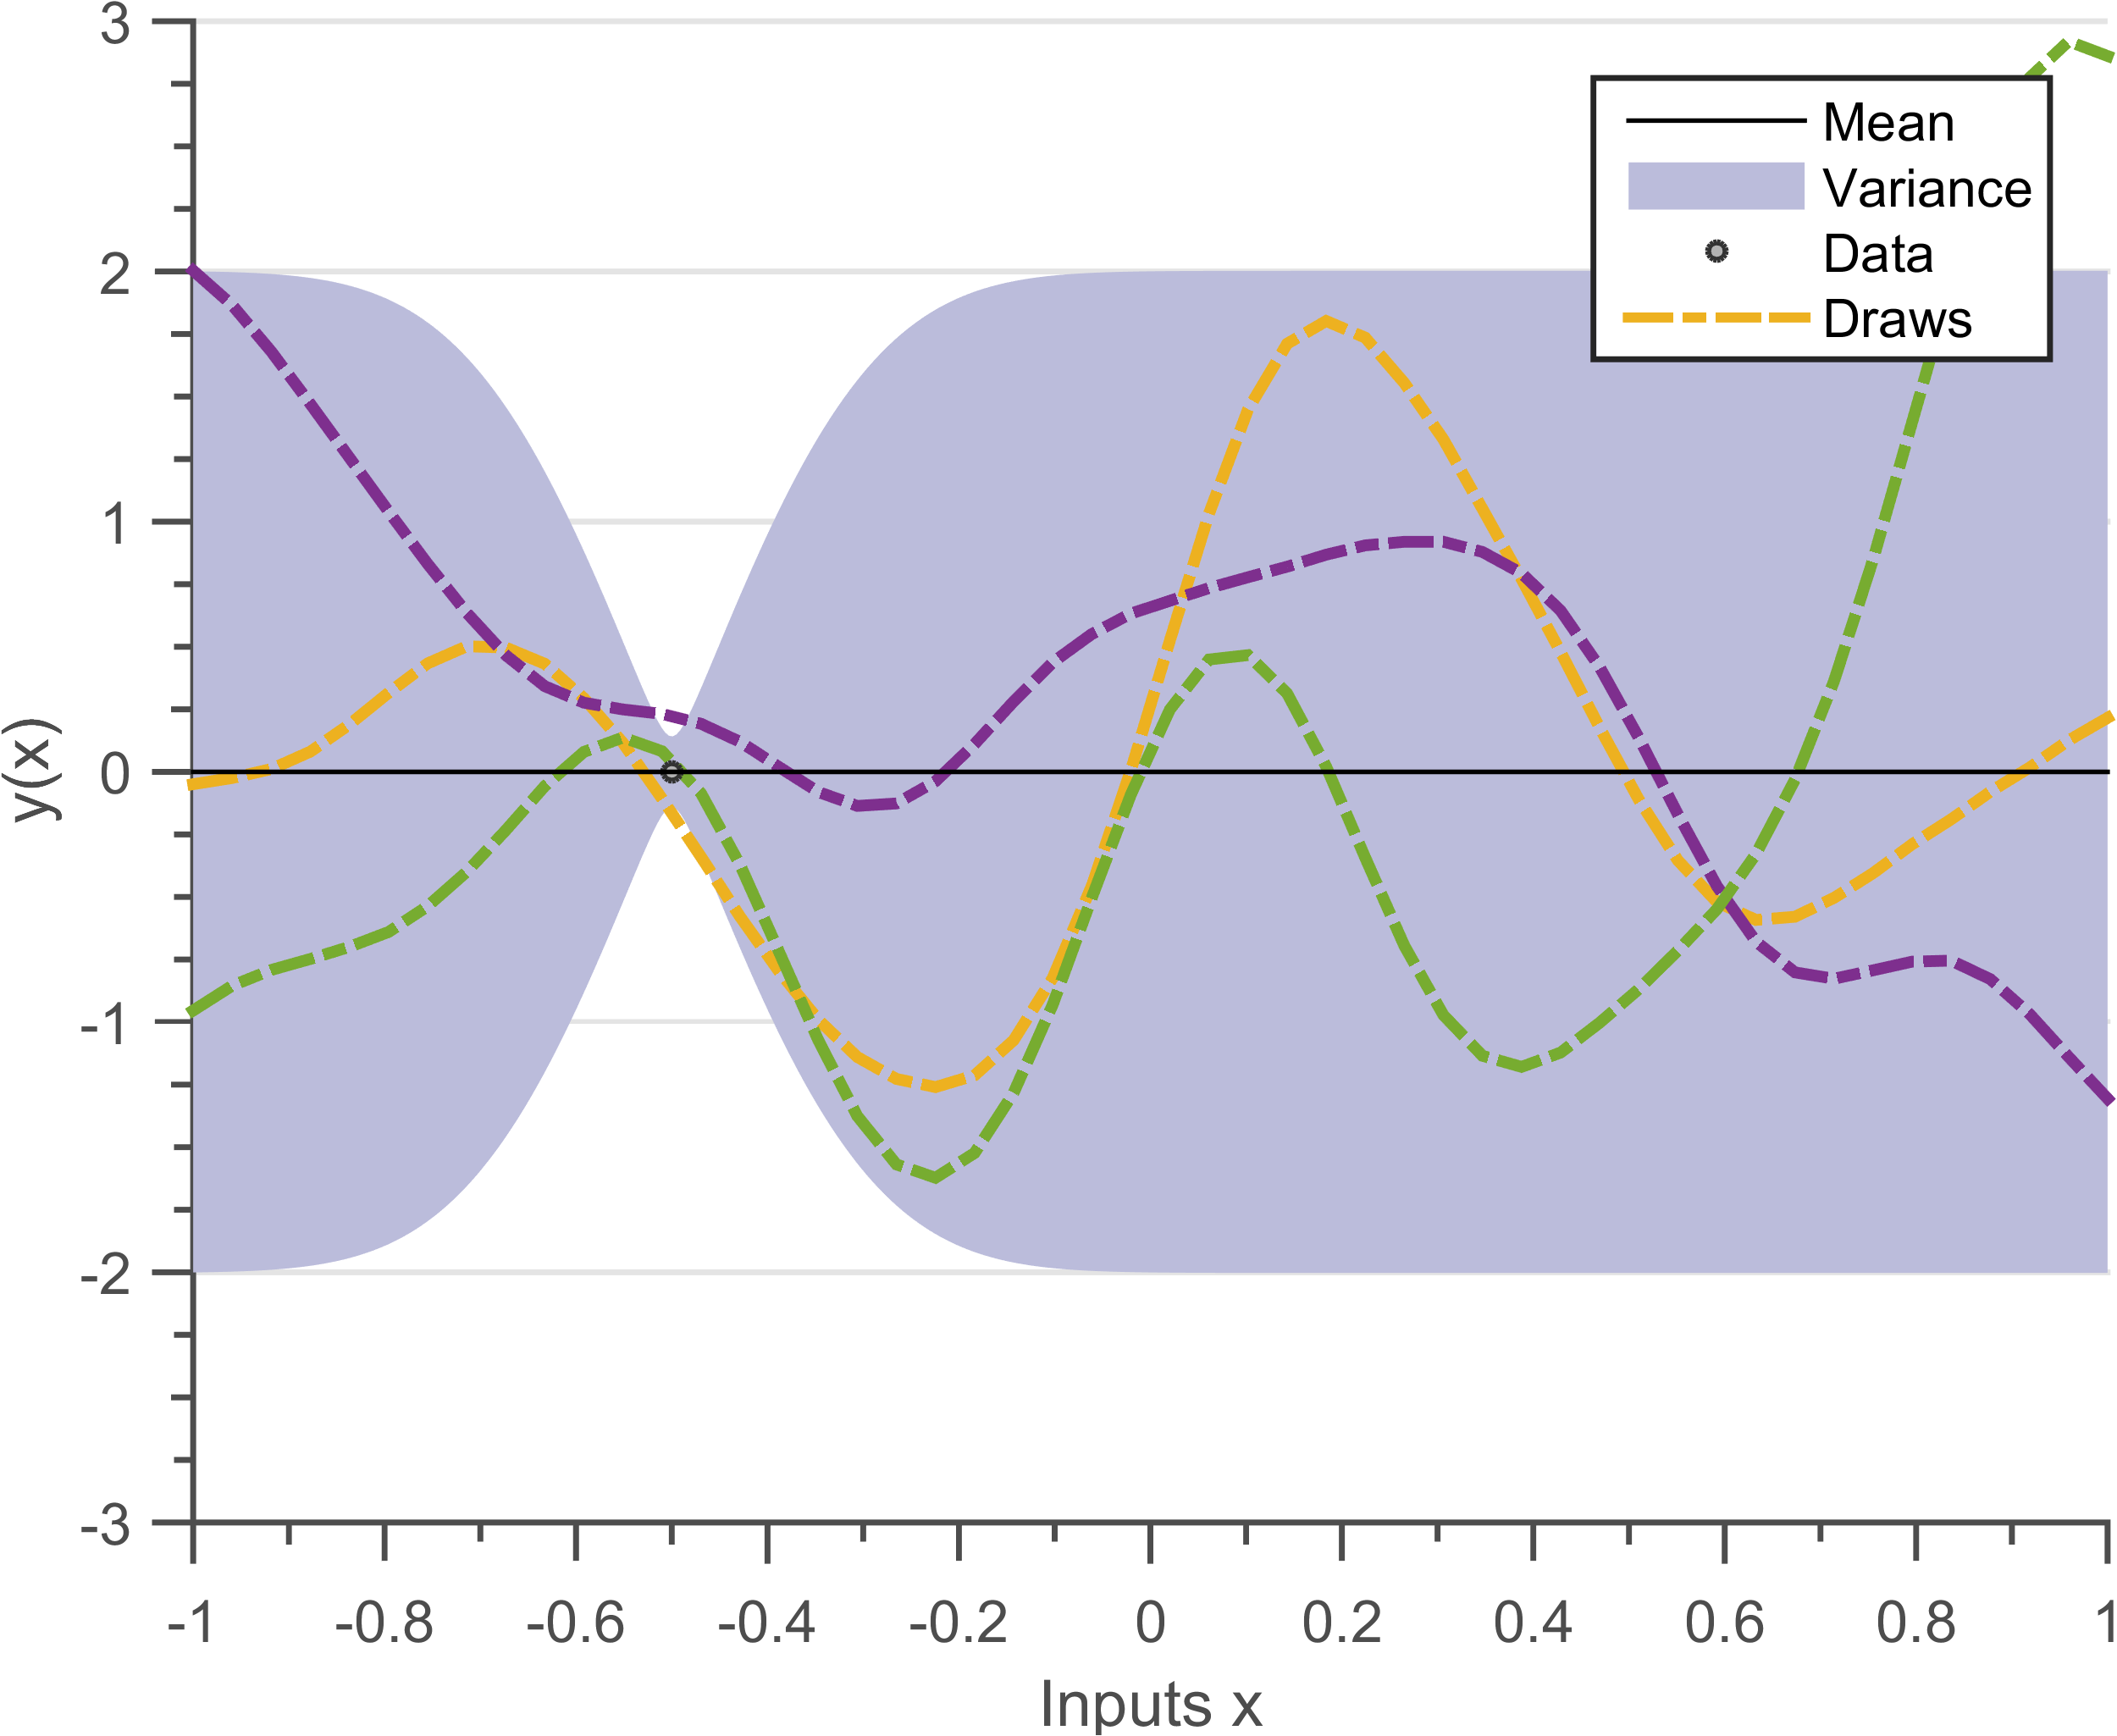
\includegraphics[width=0.45\textwidth]
        {images/posteriorSENoisy_1}
        \label{posteriorSENoisy_1}
  }\quad
\subfigure[{Posterior distribution for the case of noisy observations. Prior is a GP with mean zero, covariance as Standard Exponential (SE) Kernel with $(\theta = [1, 0.2])$ and noise as $\sigma_{n} = [0.02])$, , data set is $\{x = [-0.5, 0.33, 0.66]; f = [0, 0.5, 0.5]\}$.}]
  {
        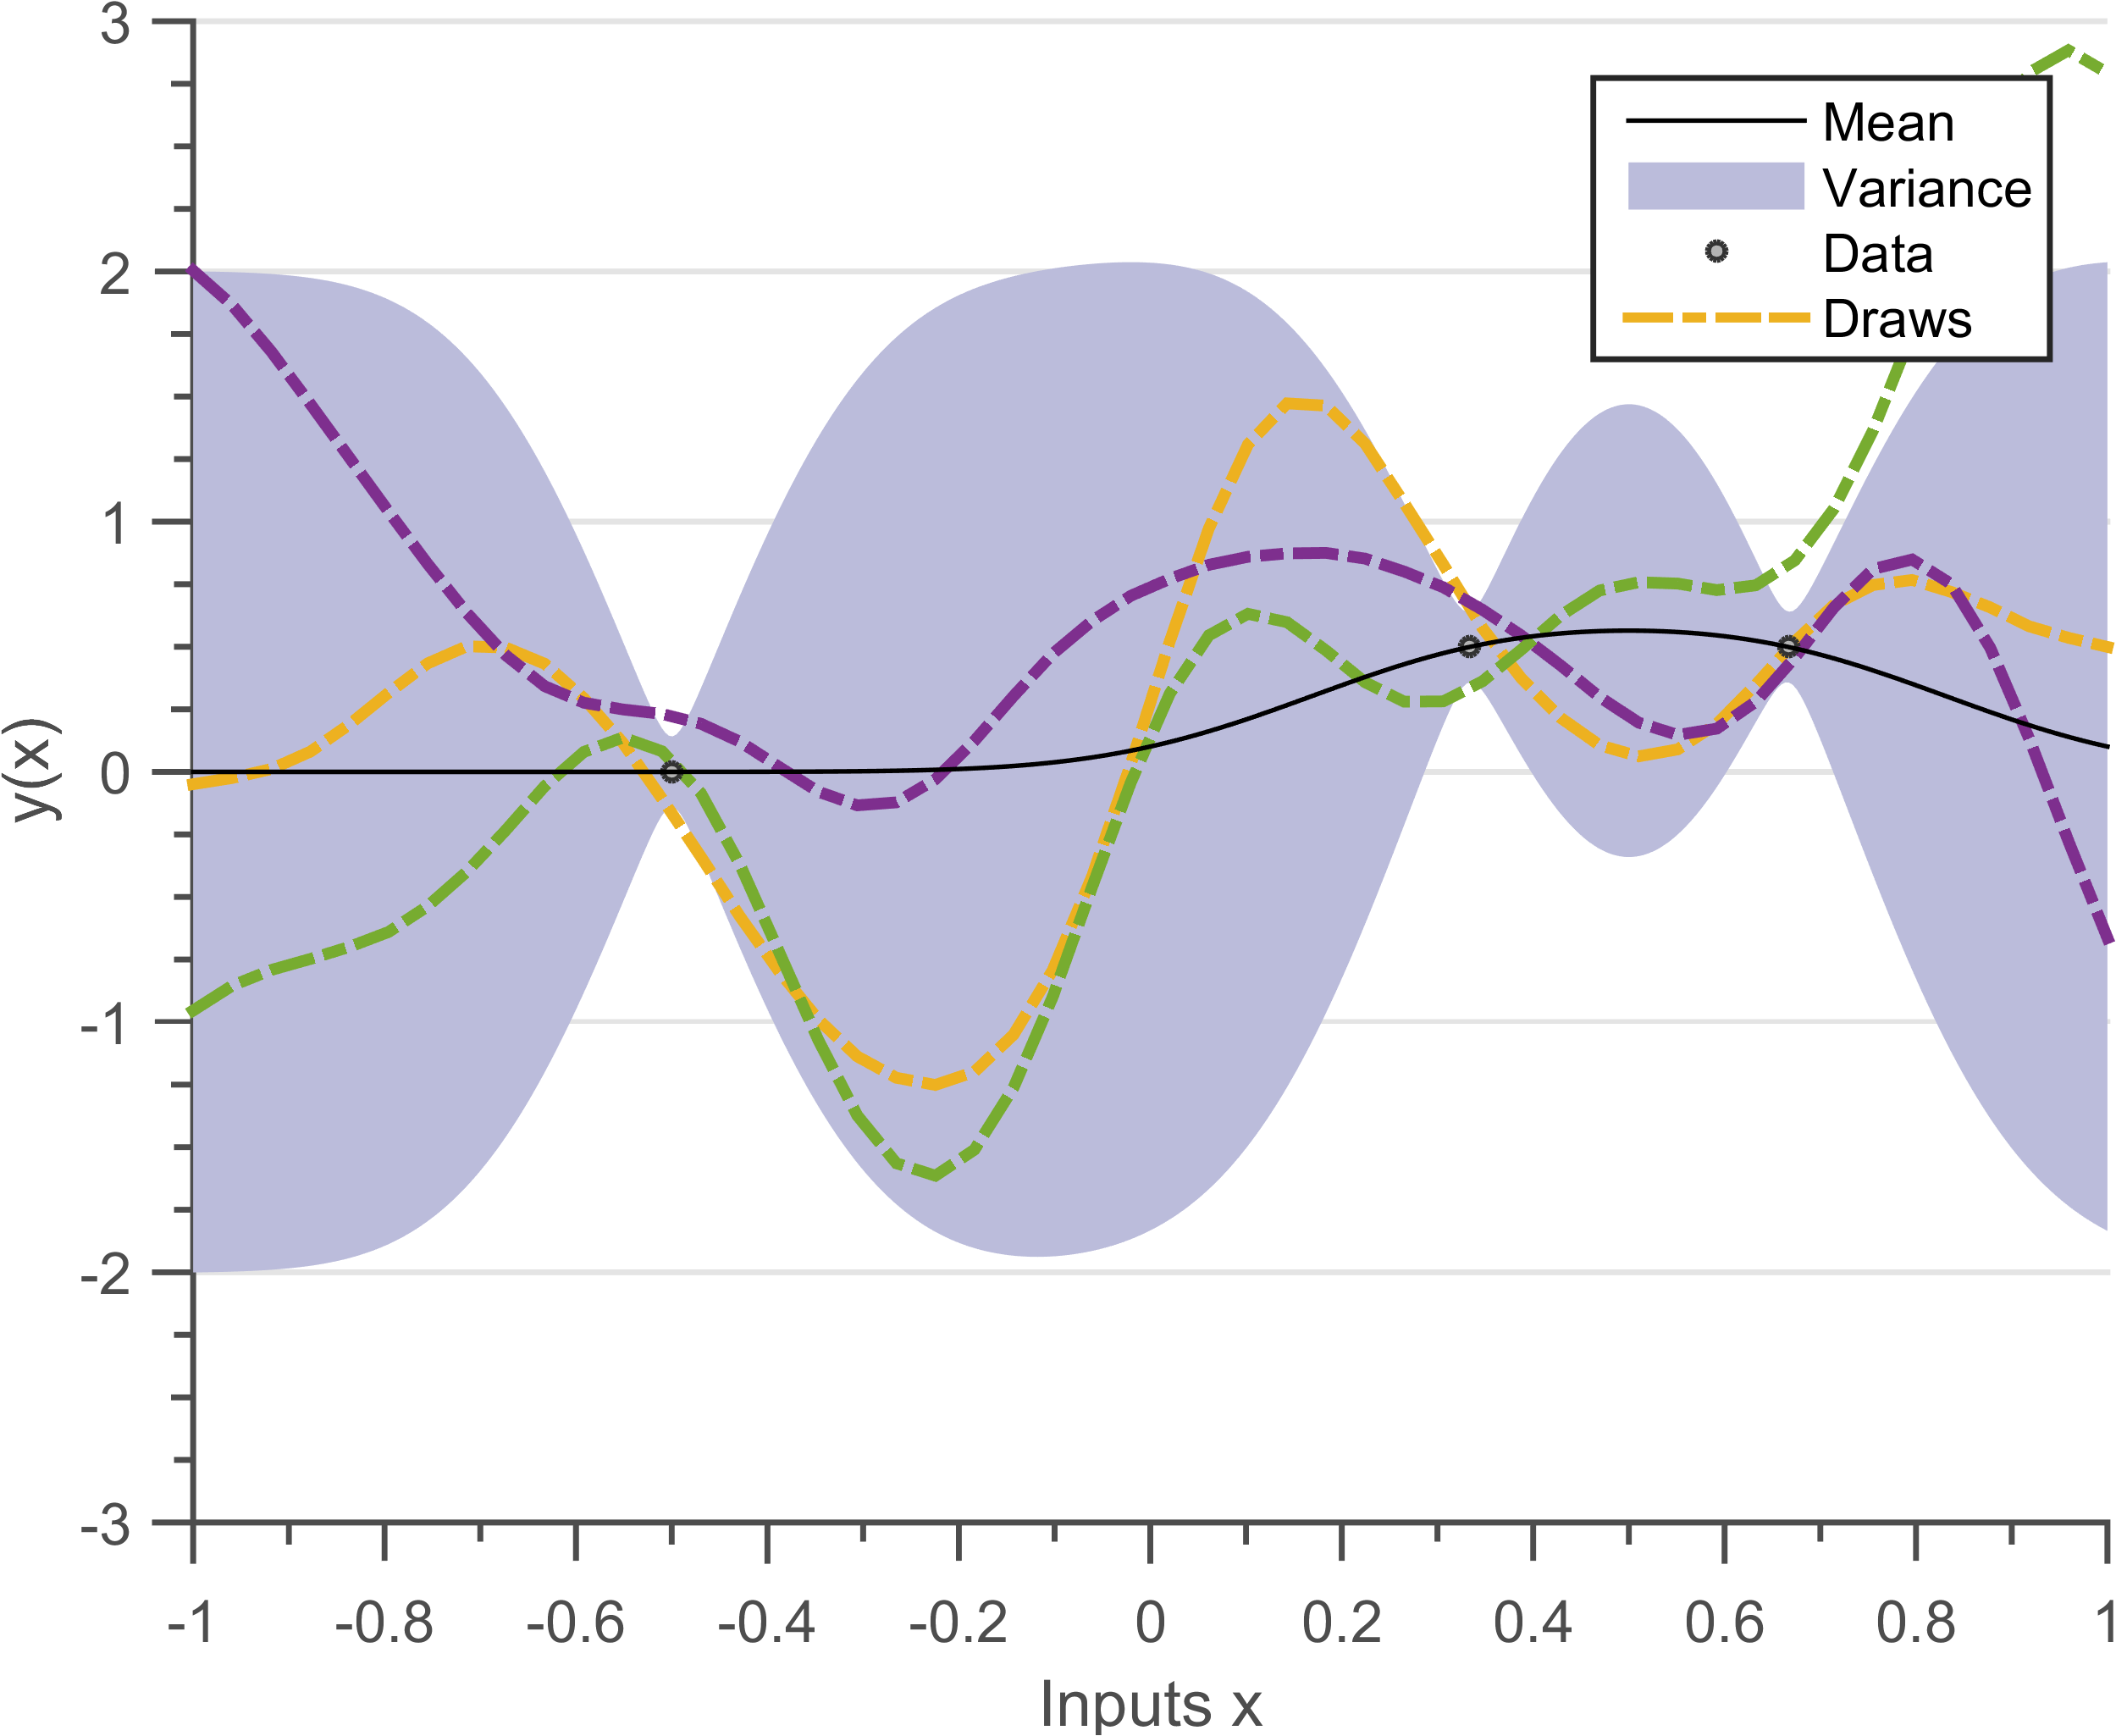
\includegraphics[width=0.45\textwidth]
        {images/posteriorSENoisy_3}
        \label{posteriorSENoisy_3}
  }\quad
  
       \caption{Prediction in the case of noisy observations. The solid black line defines the mean function, blue region defines 95\% confidence interval (2$\sigma$) distance away from the mean. The dashed lines are three functions drawn at random from a GP posterior. The mean and the draws do not pass exactly from the observation point.}
       \label{figGPNoisyPosteriors}
\end{figure}

\subsection{Interpretation of posterior}
We will now introduce a short hand notation and replace the lengthy notation $K(X, X)$ with $K_{XX}$ and $K(X, X_{*})$ with $K_{XX_{*}}$. For the case when we have only one test point $x_{*}$ we can write the predictive mean and variance in short-hand as:

  \begin{equation}\label{eqNoisyPredictiveMean}
  \mathbf{E}[f(x_{*})] = K_{Xx_{*}}^{T}( K_{XX} + \sigma^{2}_{n}I)^{-1}Y
  \end{equation}
  \begin{equation}\label{eqNoisyPredictiveCovariance}
	Cov[f(x_{*})] = K_{x_{*}x_{*}} - K_{Xx_{*}}^{T}( K_{XX} + \sigma^{2}_{n}I )^{-1} K_{Xx_{*}}
  \end{equation}

\paragraph{Precision Matrix}  
Both the predictive mean (equation \ref{eqNoisyPredictiveMean}) and predictive covariance (equation \ref{eqNoisyPredictiveCovariance}) need inverse of the covariance matrix $( K_{XX} + \sigma^{2}_{n}I)^{-1}$. The inverse of a covariance matrix is also known as a precision matrix. While the elements of a covariance matrix capture the variance and correlation information, a precision matrix contains the conditional dependence information \cite{mackay2003information}. Thus, if the $(i, j)^{th}$ element of a precision matrix is zero, the $i^{th}$ and $j^{th}$ random variables are conditionally independent. 

Calculating the precision matrix is a $\mathcal{O}\left ( N^{3} \right )$ operation for a covariance matrix of size $N$. After $N \sim 10,000$ a normal computer runs out of RAM and we thus cannot perform the inversion. Fortunately, there exist several approximations to efficiently inverse the covariance matrix and perform predictions, details are available in section \ref{chapScalingGPR}.

\paragraph{Predicted mean}
The predictive mean is a linear combination of the observations $y_{i}$, and has participation-factor of $K_{Xx_{*}}^{T}( K_{XX} + \sigma^{2}_{n}I)^{-1}$. For a SE kernel $K_{Xx_{*}}^{T}$ decreases exponentially with distance, hence observations closer to $x_{*}$ have more impact on the final prediction (equation \ref{eqNoisyPredictiveMeanLinearInY}). 
  
  \begin{equation}\label{eqNoisyPredictiveMeanLinearInY}
  \mathbf{E}[f(x_{*})] = \sum_{i = 1}^{N} K_{Xx_{*}}^{T}( K_{XX} + \sigma^{2}_{n}I)^{-1}y_{i}
  \end{equation}

The predictive mean can also be interpreted as a linear combination of the basis functions $K_{x_{i}x_{*}}$, and participation factors $( K_{XX} + \sigma^{2}_{n}I)^{-1}Y$ (equation \ref{eqNoisyPredictiveMeanLinearInBasis}). 

  \begin{equation}\label{eqNoisyPredictiveMeanLinearInBasis}
  \mathbf{E}[f(x_{*})] = \sum_{i = 1}^{N} K_{x_{i}x_{*}}( K_{XX} + \sigma^{2}_{n}I)^{-1}Y
  \end{equation}
  
This means that even though a GP represents of an infinite-dimensional vector (function), we only care about the $N$ dimensional multivariate Gaussian (section \ref{equationJointPriorNoisy}) to actually predict the mean. If the precision matrix is cached, then calculating the mean is an $\mathcal{O}\left ( N \right )$ operation.

\paragraph{Predicted variance}
The predictive variance is a combination of two terms $K_{x_{*}x_{*}}$ which is the variance due to prior assumptions and $- K_{Xx_{*}}^{T}( K_{XX} + \sigma^{2}_{n}I )^{-1} K_{Xx_{*}}$ which denotes the decrease in variance due to observations. The predictive distribution of test targets $y(x_{*})$ can be calculated by adding a noise term $\sigma^{2}_{n}$ in predictive covariance equation \ref{eqNoisyPredictiveCovariance}. 

  \begin{equation}\label{eqNoisyPredictiveCovarianceOnNoisyTarget}
	Cov[y(x_{*})] = K_{x_{*}x_{*}} - K_{Xx_{*}}^{T}( K_{XX} + \sigma^{2}_{n}I )^{-1} K_{Xx_{*}} + \sigma_{n}^{2}
  \end{equation}
  
We observe that the predicted variance in not dependent on the observations $y$, this is one of the flaws in GP regression. Since the assumption that the dataset $(\mathcal{D})$ comes from a GP might not necessarily be true, the predicted variance can poorly represent the model error. Hence, predicted variance is not necessarily a measure of model error but an efficient method to track uncertainties arising from the prior assumption and non-continuous observations \cite{shah2014student}.

The mean and variance are highly dependent on the kernel hyper-parameters. In order to automatically learn the hyper-parameters, we must perform model selection. Section \ref{secHyperParameter} details how to fine-tune hyper-parameters to find an optimal prediction.

\section{Choosing Hyper-parameters}\label{secHyperParameter}
Since the properties of functions under a GP are controlled by the functional form of the covariance kernel and its hyper-parameters, model selection amounts to choosing a functional form and learning the hyper-parameters $\theta$ from data. In this section we discuss how to select an optimal model by tuning hyper-parameters for a given covariance function. Please refer to chapter \ref{chapAddingEquationsInGP} for discussion on how to choose covariance functions. 

Figure \ref{figGPRMarginal} demonstrates that choosing optimal hyper-parameters is very vital for accurate prediction. Figure  \ref{figGPRMarginal} compares the posterior distributions obtained for SE priors with 2 different hyper-parameters. We observe that the mean of figure \ref{subFigPosterior1} passes through all the observed data points but is more complex. The mean in figure \ref{subFigPosterior3} is a smooth function but does not fit the data properly. 

  \begin{figure}[!ht]
  \centering
    \subfigure[{Posterior between SE prior with hyper-parameters $(\theta = [0.35, 0.05]; \sigma_{noise} = 0.01)$ and data. }]
    %$\log (ML) = -35.3$]
  {
        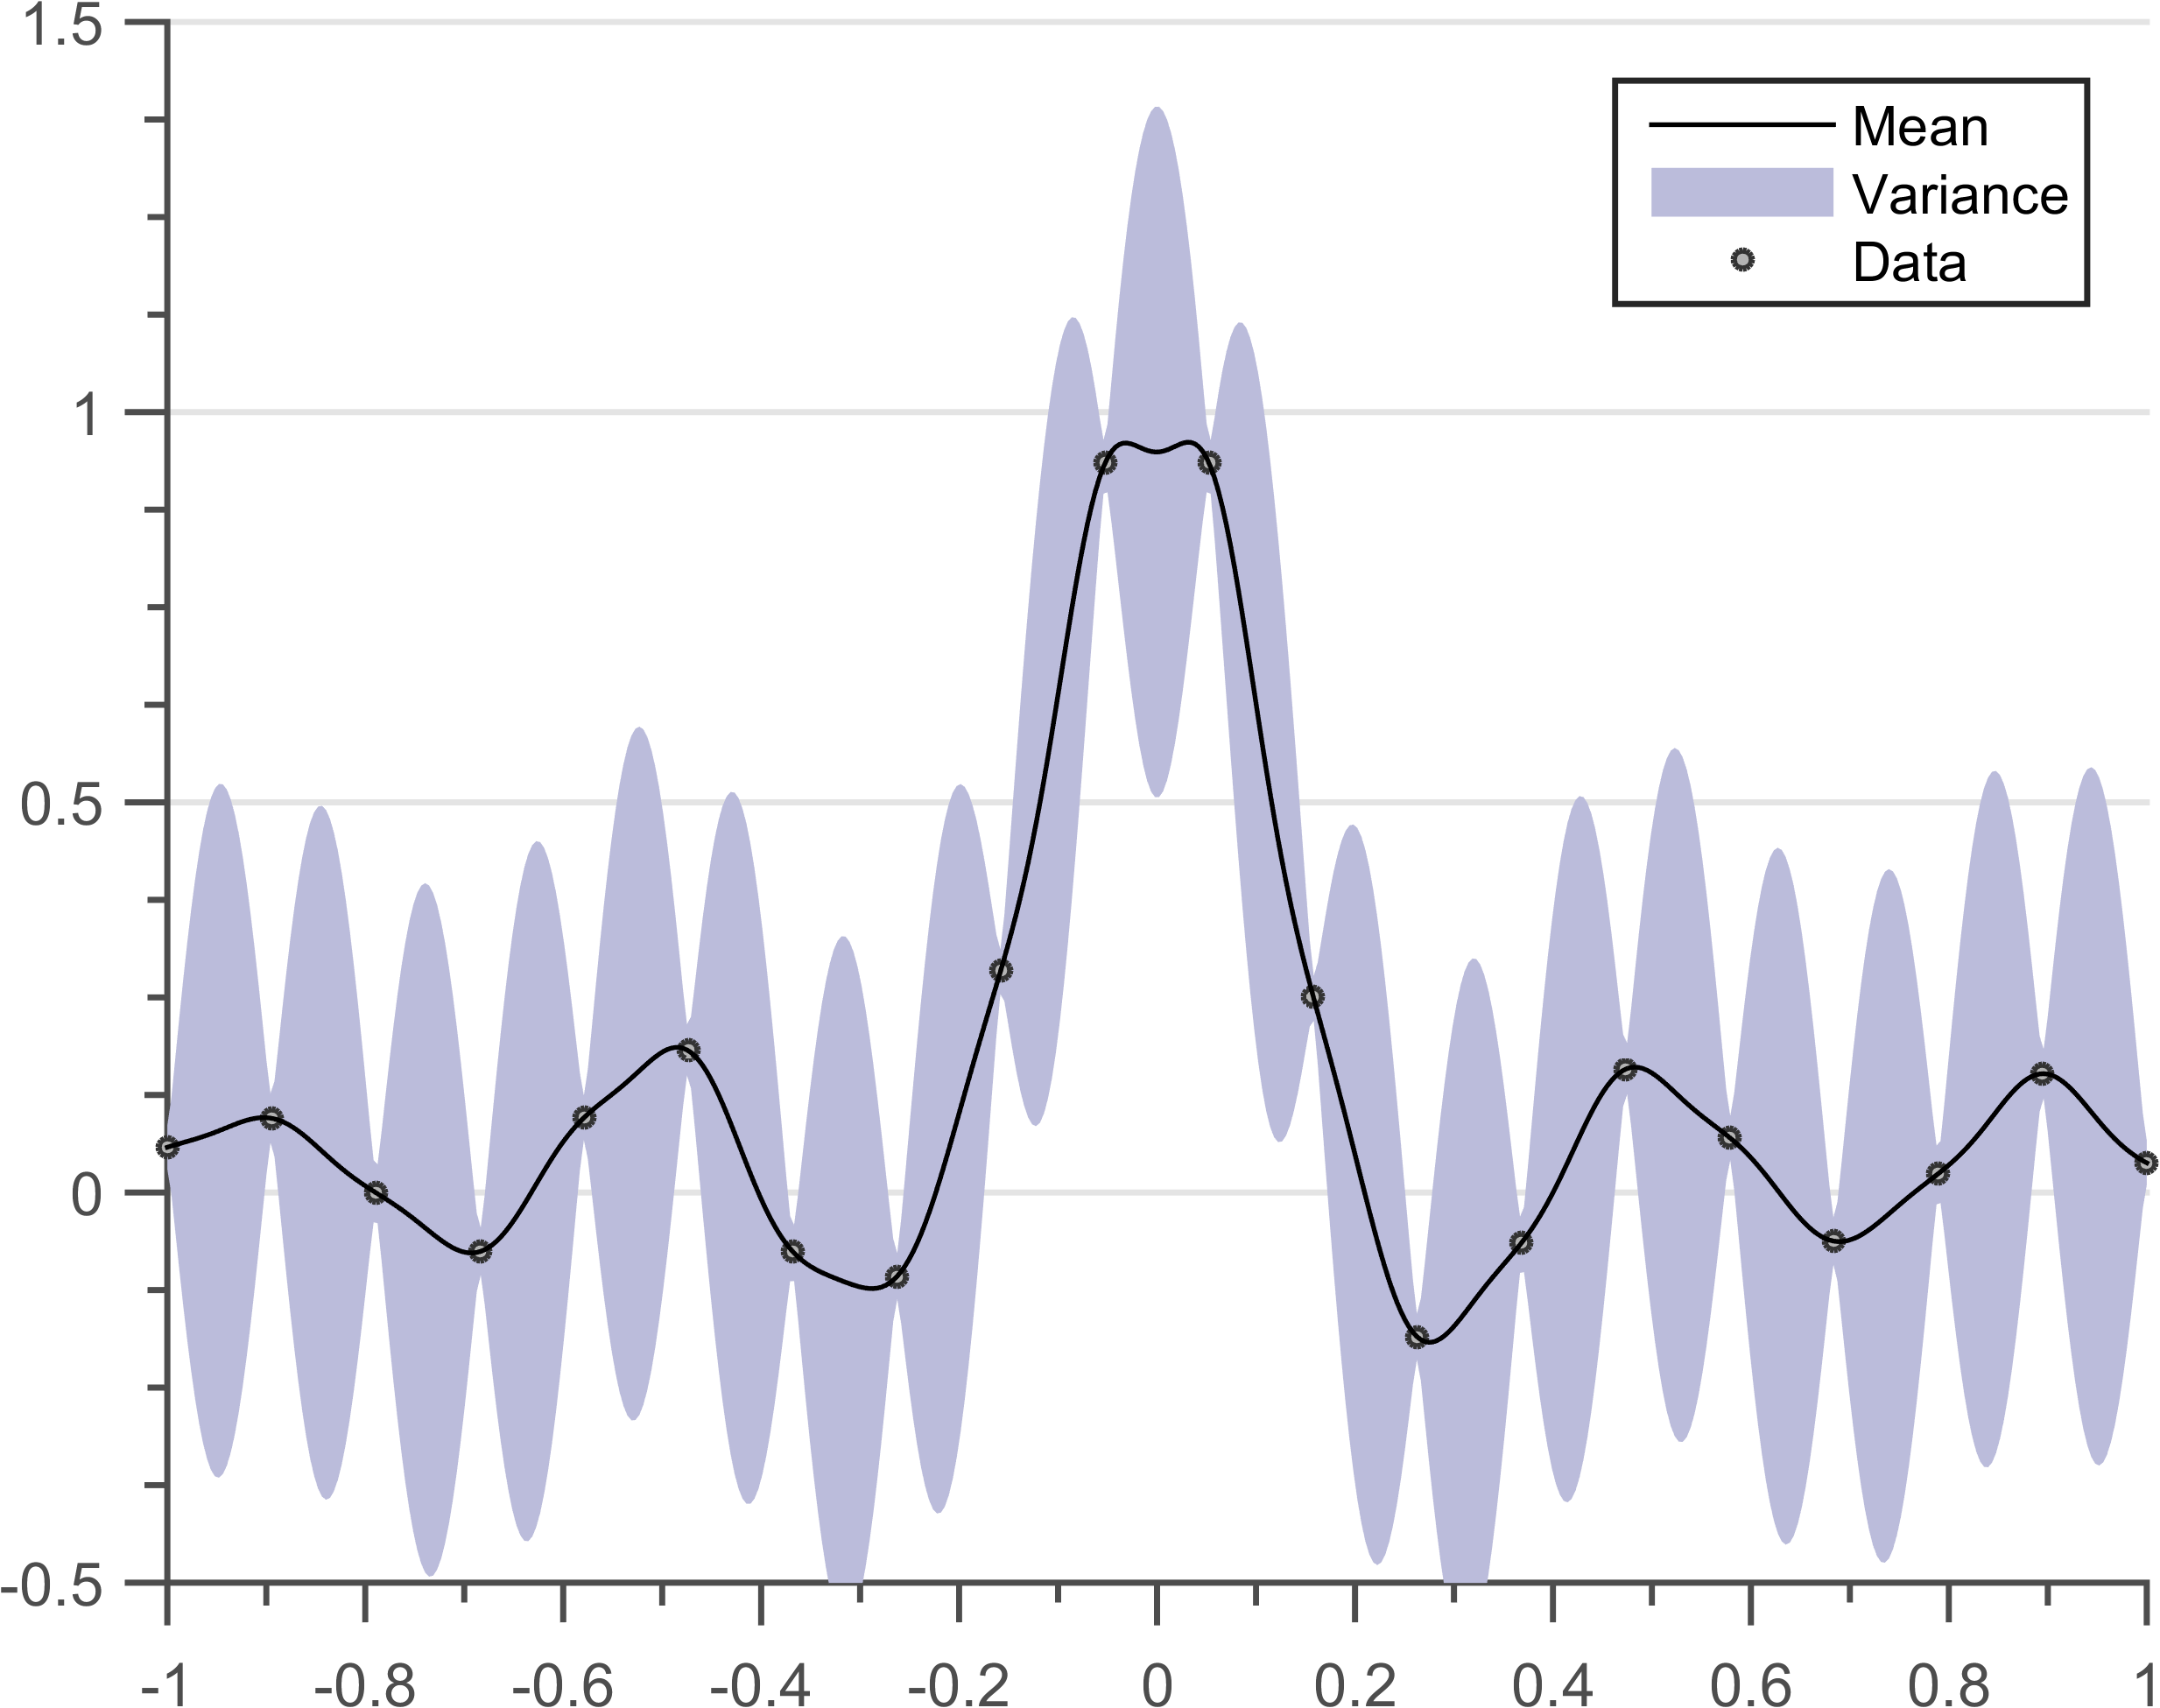
\includegraphics[width=0.45\textwidth]
        {images/posteriorSE1}
        \label{subFigPosterior1}
  }\quad
\subfigure[{Posterior between SE prior with hyper-parameters $(\theta = [0.35, 0.5]; \sigma_{noise} = 0.01)$ and data. }]
%$\log (ML) = -8.2$}]
  {
        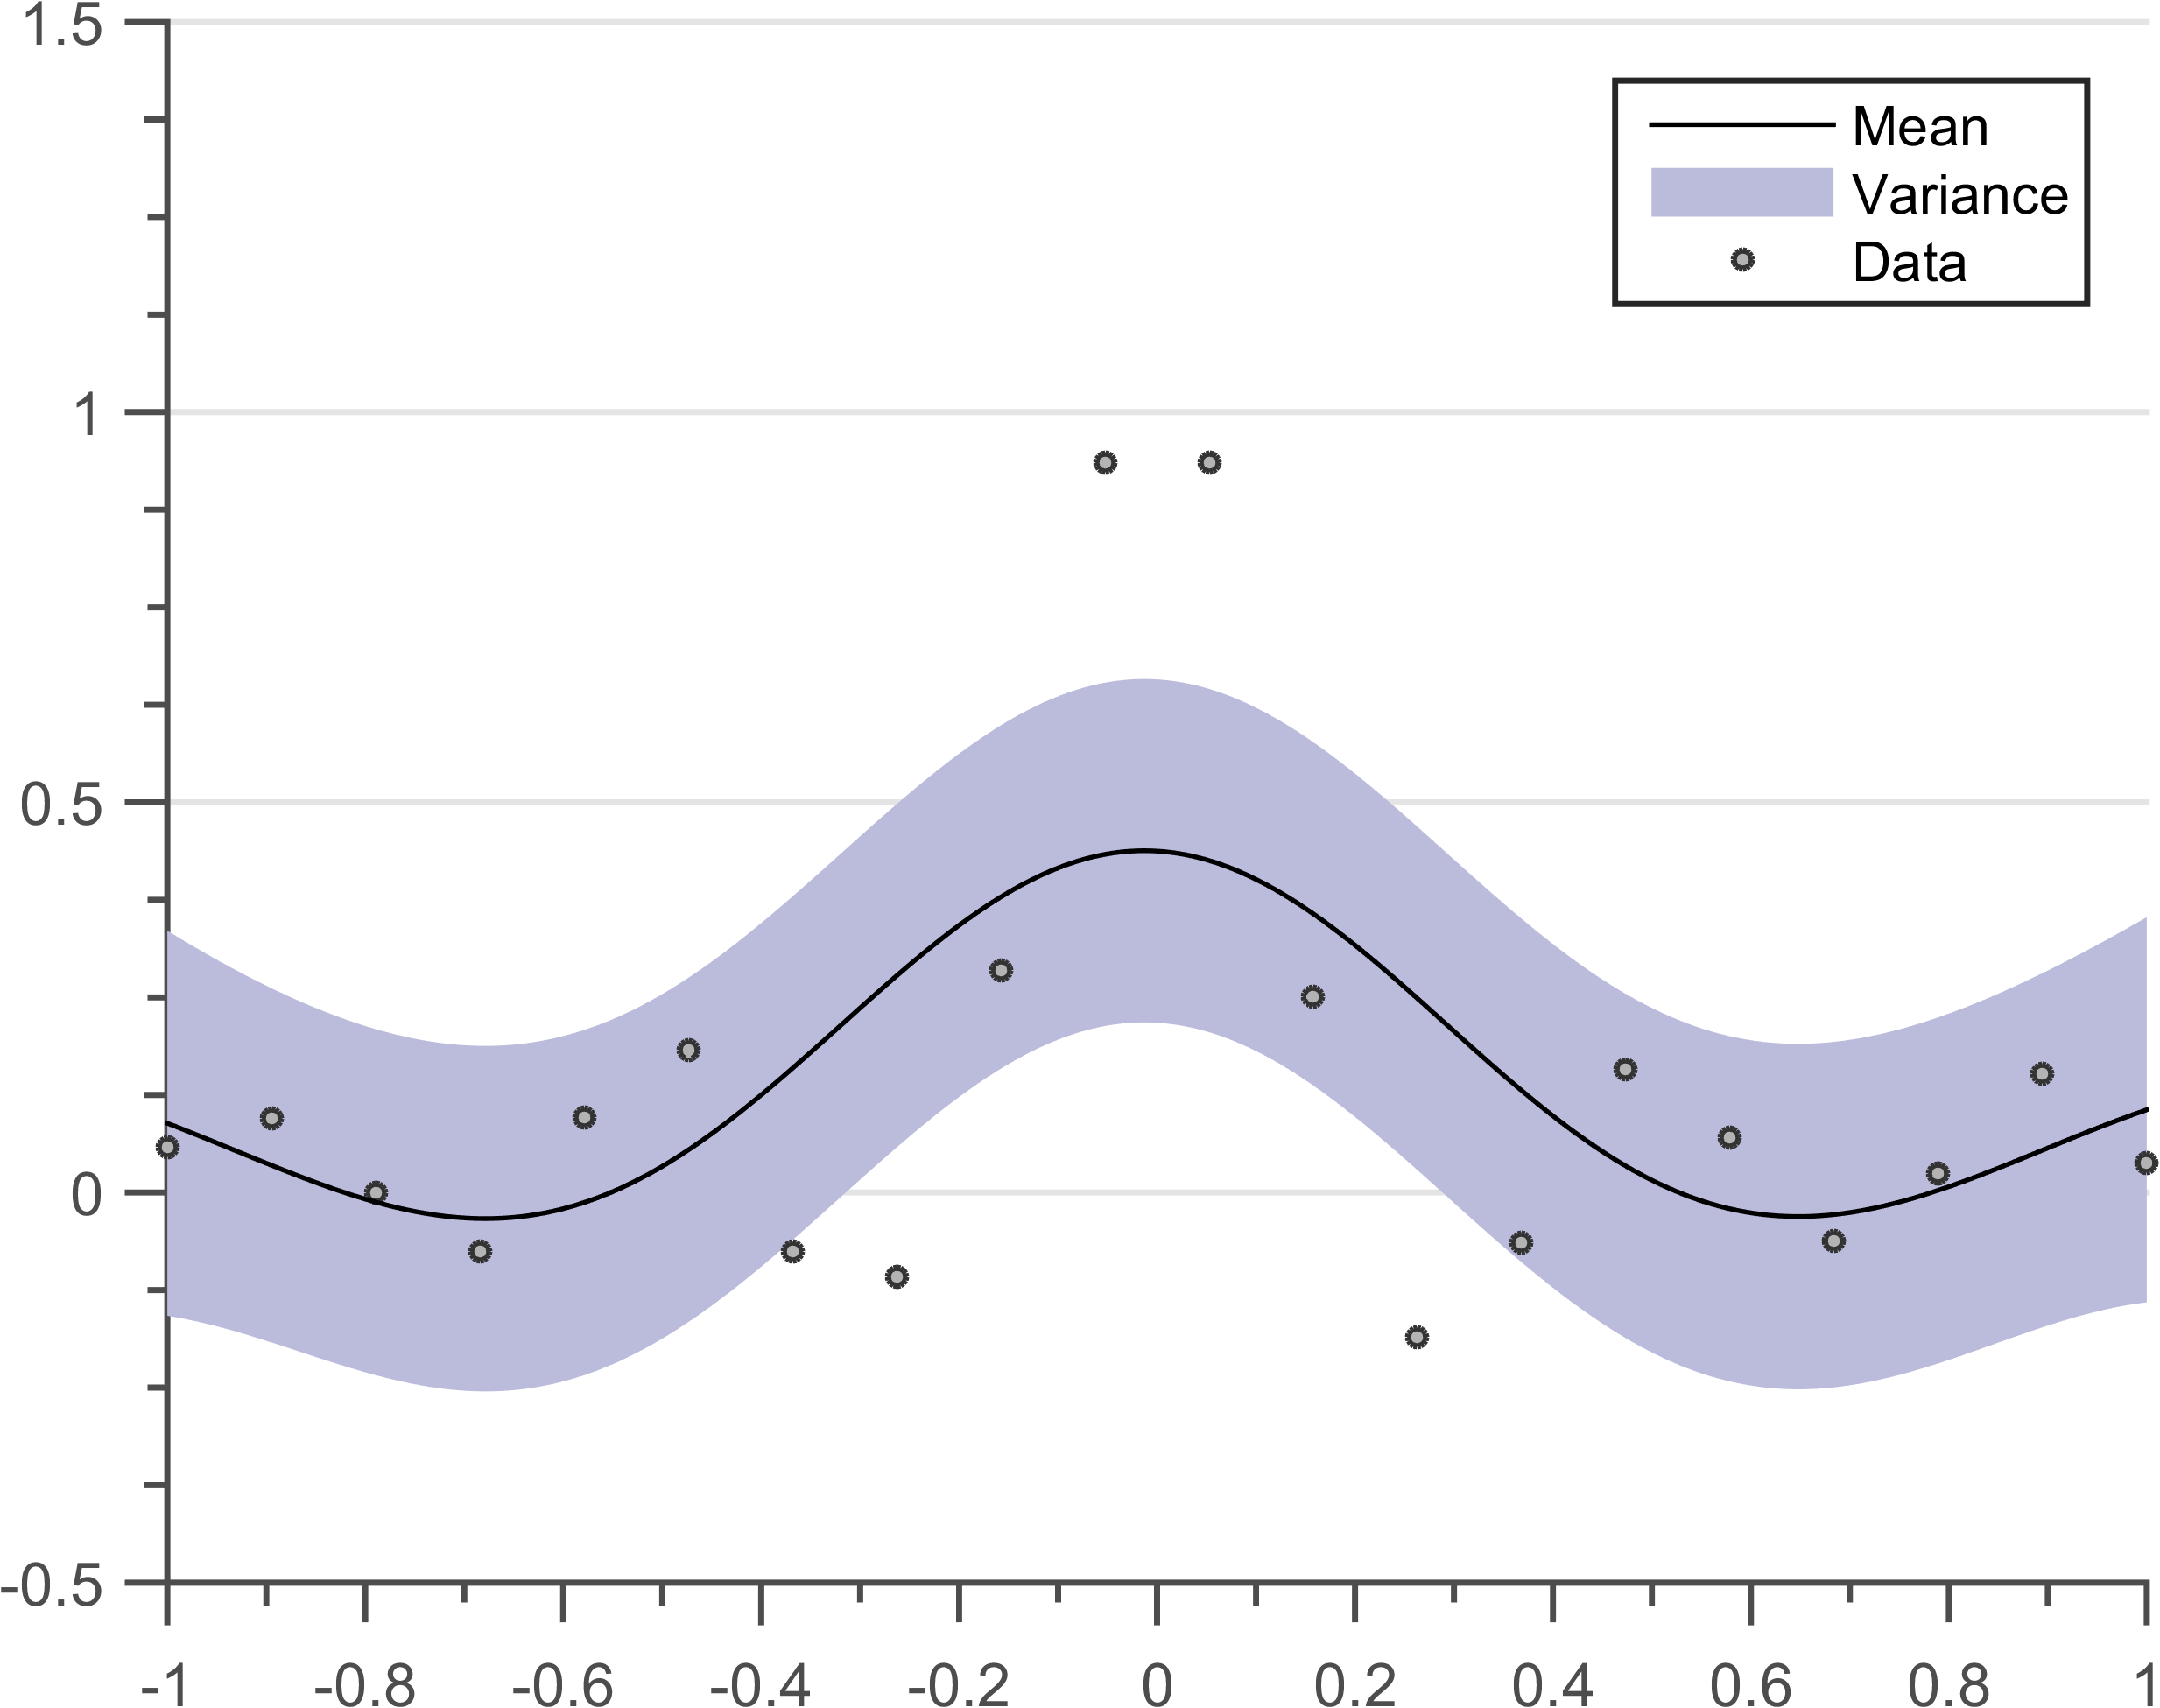
\includegraphics[width=0.45\textwidth]
        {images/posteriorSE3}
        \label{subFigPosterior3}
  }\quad
       \caption{Posteriors for 2 different sets of hyper-parameters. Solid black line defines the mean function, blue region defines 95\% confidence interval (2$\sigma$) distance away from mean. }\label{figGPRMarginal}
\end{figure}

Since hyper-parameters control the family of functions in the hypothesis space and are equivalent to parameters $w$, in a pure Bayesian framework we should put a prior over our hyper-parameters $\Pr[\theta]$ and use Bayes Rule to estimate the posterior $\Pr[\theta \mid \mathcal{D}]$ over our data set. However, this approach becomes intractable and several sampling schemes have been proposed to calculate the posterior of hyper-parameters \cite{osborne2010bayesian, neal2011mcmc}.

Another method to find the optimal hyper-parameters is by performing Cross-Validation (CV). CV procedure is to split the experimental design set into two disjoint sets, one is used for training and the other one is used to monitor the performance
of the surrogate model. A particular case of CV is the Leave-One-Out (LOO) where test sets are obtained by removing one observation at-a-time. Although this can be time-consuming, there are computational short-cuts available for this scheme \cite{rasmussen2006gaussian, dubrule1983cross, le2013multi}. 

In this manuscript we neither put a prior over our hyper-parameters nor use LOO-CV for choosing hyper-parameters. We use the marginal likelihood also called evidence to find optimal hyper-parameters \cite{mackay2003information}. The probability of generating the observations $(Y)$ at the points $(X)$ from a prior (defined by $k(x_{1}, x_{2}, \theta)$) is called the marginal likelihood $\Pr[Y \mid X, \theta]$. In other words, marginal likelihood is the probability that our data set $\mathcal{D}$ was generated from a particular prior. Hence, when we maximize a marginal likelihood we are finding the best prior that could generate our data set. Using equation \ref{equationMeanZeroGPNoisydefinition} and \ref{equationJointPriorNoisy} we get:

\begin{equation}\label{equationMarginalLikelihood}
\begin{aligned}
\Pr[Y(X) \mid X, \theta, \sigma_{n}] & = \mathcal{N}(0 , K(X, X') + \sigma^{2}_{n}I)  \\
& = \frac{1}{\sqrt{(2\pi)^{N/2} K_{XX}}} exp^{-\frac{1}{2}Y^{T}K_{XX}Y}
\end{aligned}
\end{equation}

 Directly, maximizing the marginal likelihood with respect to the hyper-parameters can be inefficient. This is because the marginal likelihood does not vary significantly with the hyper-parameters. Hence to speed up the optimization process we generally maximize the log of marginal likelihood. 

  \begin{equation}\label{eqExactNLML}
\log(\Pr [Y \mid X, \theta ]) = -\frac{1}{2}Y^{T}[K_{XX}+ \sigma_{noise}^{2}I]^{-1}Y - \log\left |  K_{XX}+ \sigma_{noise}^{2}I\right | - \frac{n}{2}\log(2\pi)
  \end{equation}
  
The marginal likelihood is a trade-off between a data-fit term $(\frac{1}{2}Y^{T}K_{XX}^{-1}Y)$ and a model complexity term $(\log\left |  K_{XX}\right |)$. The optimization of ML($\theta$) provides the best compromise in terms of explaining the existing data set \{($x_{i}, y_{i}$)\} and the initial assumptions encoded in the prior. 

Figure \ref{subFigmaximizingMarginalLikelihood} shows the contours of marginal likelihood with respect to length-scale $\theta_{lengthScale}$ and noise $\sigma_{n}$ hyper-parameters. The data set is same as used in figure \ref{figGPRMarginal} and the prior is a zero mean with SE kernel. Figure \ref{subFigPosteriorOptimized} shows the posterior for same data set as used in figure \ref{figGPRMarginal} but for the hyper-parameters where marginal likelihood is maximum. The marginal likelihood could have multiple maximas in the space of hyper-parameters, hence care should be taken while initializing hyper-parameters for optimizing the log of marginal likelihood. 


  \begin{figure}[!ht]
  \centering
    \subfigure[{Marginal likelihood contours for varying noise and length-scale parameter. The amplitude hyper parameter is $(\theta_{amplitude} = [0.35])$.  Also shown on the figure are locations of hyper-parameters for figures \ref{subFigPosterior1} and \ref{subFigPosteriorOptimized}.}]
  {
        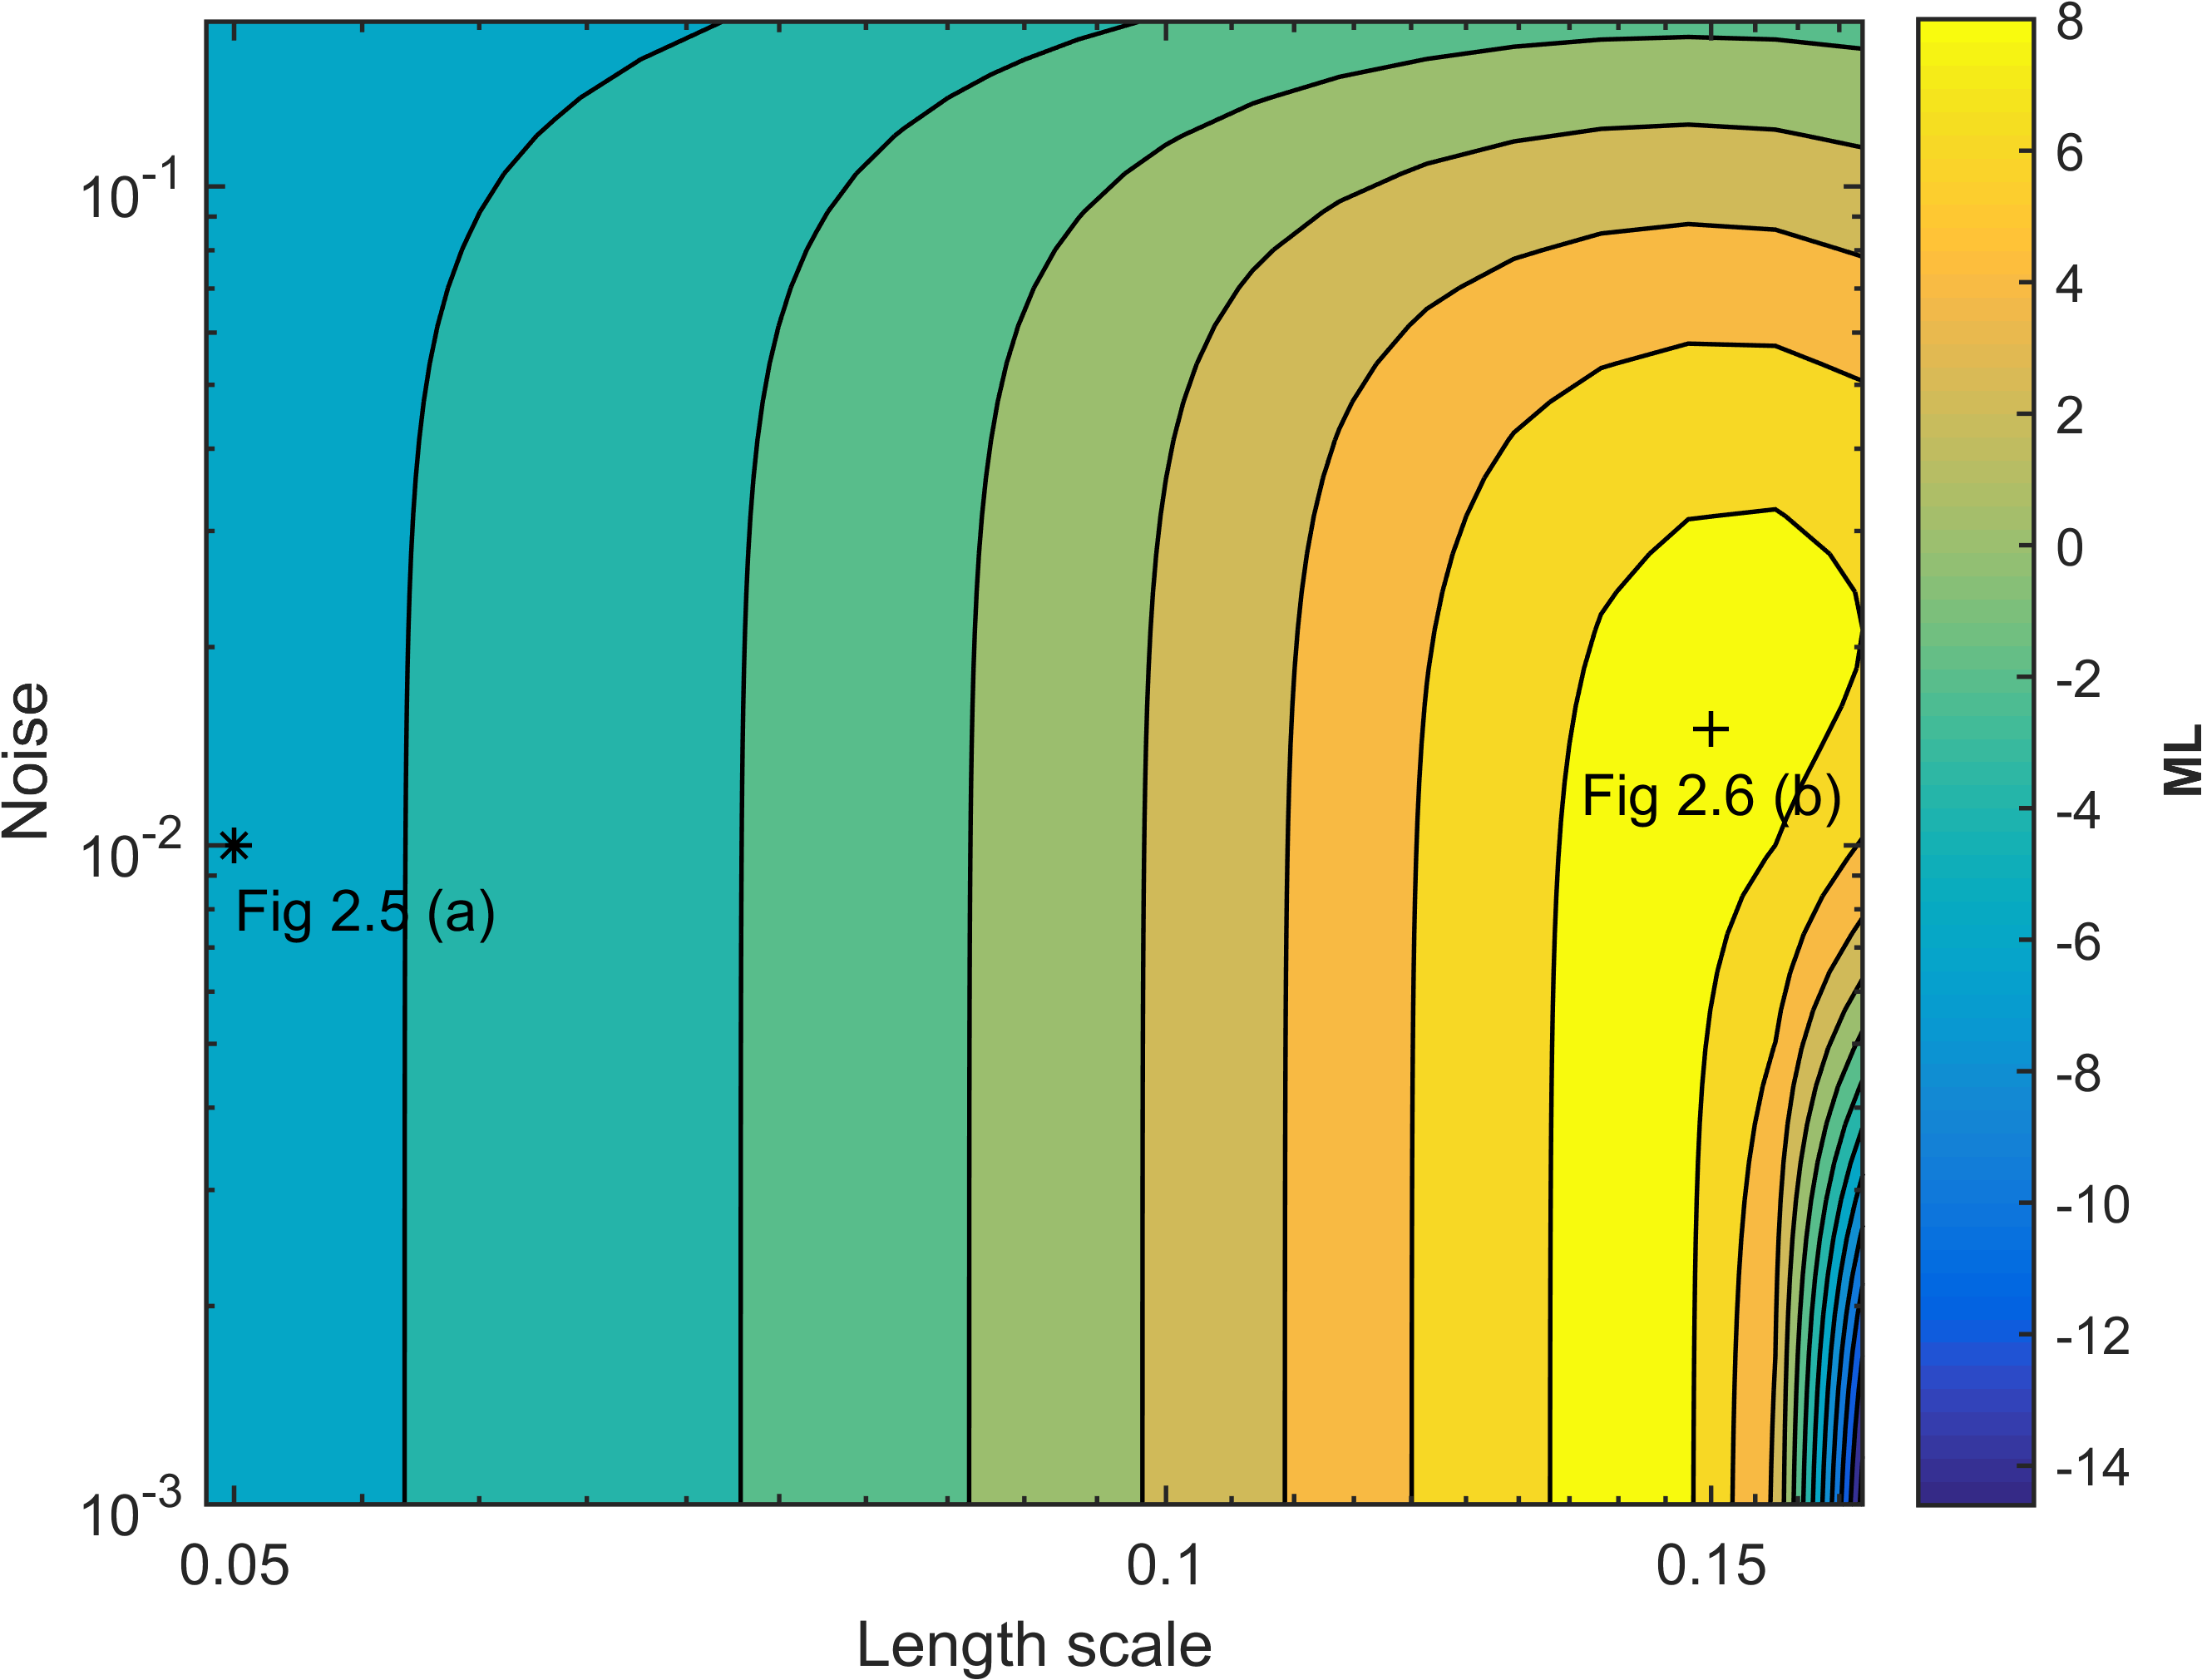
\includegraphics[width=0.45\textwidth]
        {images/maximizingMarginalLikelihood}
        \label{subFigmaximizingMarginalLikelihood}
  }\quad
  \subfigure[{Posterior between SE prior with optimized hyper-parameters $(\theta = [0.35, 0.15]; \sigma_{noise} = 0.015)$ and data. $\log( ML) = 8.04$. Solid black line defines the mean function, blue region defines 95\% confidence interval (2$\sigma$) distance away from mean.}]
  {
        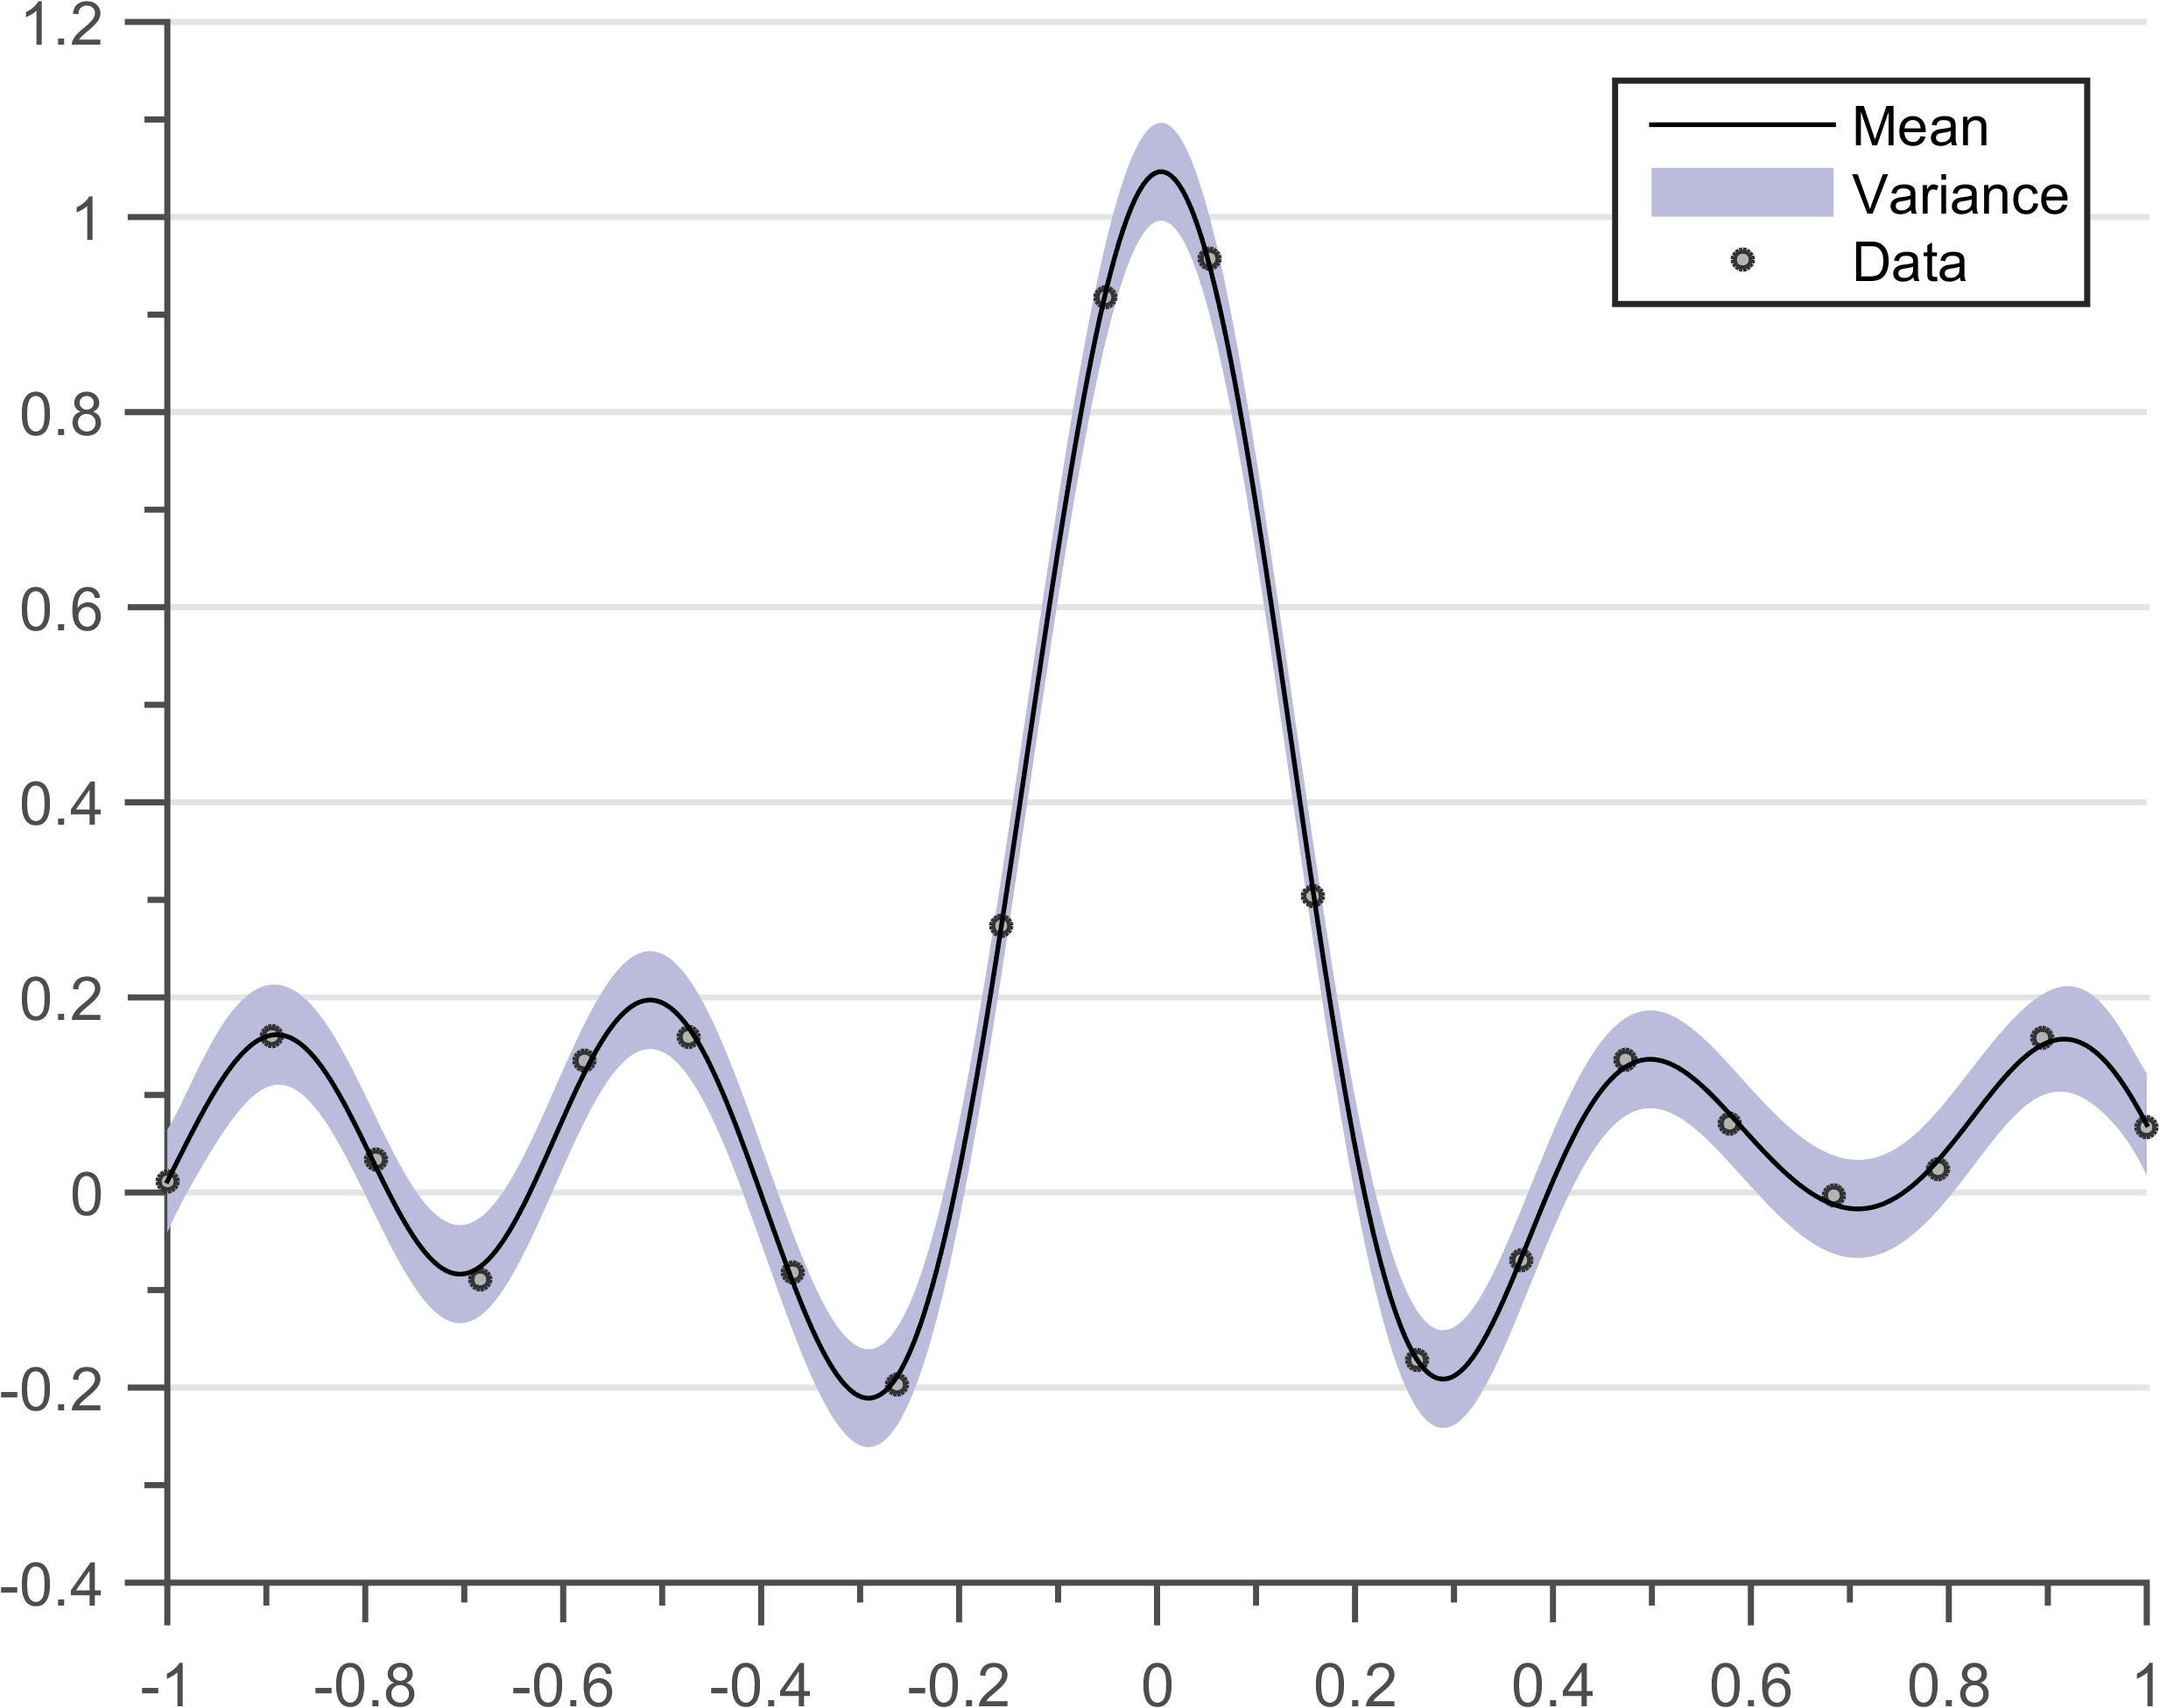
\includegraphics[width=0.45\textwidth]
        {images/posteriorSE}
        \label{subFigPosteriorOptimized}
  }\quad
       \caption{Maximizing marginal likelihood}\label{figGPRMarginalOptimized}
\end{figure}

\section{Discussion}\label{secCH2Discussion}
In this chapter we provide a brief introduction on how to perform Regression with GPs. GPs are the ideal candidate for regression due to their marginalization property, which makes them computationally tractable. Even if GPs define an infinite dimensional random vector, inference on a few points does not require the presence of infinitely other points. This makes drawing functions, calculating posterior distribution and automating selection of hyper-parameters computationally feasible. Thereby making GPs an ideal candidate for defining a Prior distribution in a Bayesian Regression framework. 

The section \ref{secPrior} details the key constituents of a GPs. A GP can be completely parametrized by its mean and covariance function. While, the trend of a GP is defined by its mean function, the structure of its constituent functions is defined by the covariance function. Normally the mean of a GP can be assumed to be zero, since an extra term in the covariance function can represent the mean function. Hence the problem of learning in a GP is exactly the problem of finding suitable properties of the covariance function (subsection \ref{subSecCH2Covariance}). Once a function form of covariance is chosen we can calculate the Gram matrix at desired points and use it to draw random functions from our prior (subsection \ref{subSecSamplingFunctionsGPPrior}). 

The next section \ref{secPosterior} describes how to calculate the posterior distribution. The posterior is the conditional distribution $(\Pr[f(x_{*}) \mid Y, X, \theta])$ for an assumed Prior distribution $(\Pr[f] = GP(0, k(x_{1}, x_{2}, \theta))$ and a set of observed data points $(\mathcal{D} = {X, Y})$. Again, due to the Gaussian assumption the conditional probabilities are all computationally tractable and can be calculated using a few matrix operations, side-stepping the computational burden of performing iterative sampling. Calculating the posterior is easy both in the absence (subsection \ref{subSecPosteriorNoiseFree})and presence (subsection \ref{subSecPosteriorNoisy}) of noise in observations. 

Given a functional form of the covariance, section \ref{secHyperParameter} shows the importance of choosing the correct hyper-parameters. In a pure Bayesian framework the posterior distribution of the hyper-parameters should be calculated ($\Pr[\theta \mid \mathcal{D}]$), but this is computationally intractable needing several iterations for calculation of integrals. A common practice in the community is maximizing the marginal likelihood to automatically choose the hyper-parameters. Marginal likelihood is the probability of a prior distribution $\Pr[f] = GP(0, k(x_{1}, x_{2}, \theta)$ generating the observations $\mathcal{D}$. Hence maximizing the marginal likelihood gives the optimal set of hyper-parameters for a functional form of covariance function (figure \ref{figGPRMarginalOptimized}). 

Calculating the precision matrix $[K_{XX}+ \sigma_{noise}^{2}I]^{-1}$ is an important task in calculating the marginal likelihood (equation \ref{}), posterior mean (equation \ref{}) and covariance (equation \ref{}). Unfortunately, this task has a computational complexity of $\mathcal{O}\left ( N^{3} \right )$ and memory footprint of $\mathcal{O}\left ( N^{2} \right )$. Putting an upper limit of $N \sim 10^4$ on the number of data points, a standard laptop cannot store such a big matrix for inversion \footnote{The computer runs out of memory before we run out of patience :p}. The next chapter describes few methods of performing approximating inference which scales GPs to $N \sim 10^6$ or more data points. 
\chapter{Scaling up Gaussian Process Regression}
\label{chapScalingGPR}

The GP regression approach as mentioned in earlier chapter is intractable for large data sets. For a data set of size \(N\) the covariance matrix \(K_{XX}\) is of size \(N \times N\),  where \(\mathcal{O}\left ( N^{3} \right )\) time is needed for calculating the precision matrix and \(\mathcal{O}\left ( N^{2} \right )\) memory for storage. Since, inverting the covariance matrix takes considerable amount of time and memory, almost all techniques to scale up GP regression try to approximate the inversion of Gram matrix \(K_{XX}\). 

Let us take the example of an SE kernel, for a large value of length-scale the Gram matrix (\(K_{XX}\)) is spread out and has a rank lower than  \(N\) (figure \ref{subFigSEPrior_2}). Due to this low-rank characteristic the Gram matrix can be approximated as a lower rank form reducing the cost of inverting the Gram matrix. In the GP literature sparse approximations (section \ref{secSparseApprox}) use a set of inducing points to compress the information of the several observations through the low-rank approximation. 

For the same SE kernel if the length-scale tends to a low value the Gram matrix is not of low-rank but tends to a diagonal matrix (figure \ref{subFigSEPrior_1}). In the GP literature the mixture of experts (section \ref{secDgp}) methodology exploits the block diagonal nature of the Gram matrix by distributing data points into a subset of experts, assuming independence across experts and distributing the calculations into several batches. The first regime suggests global (numerical) low-rank approximations while the second regime suggests local block-diagonal approximations \cite{march2015askit, chenhan2016inv}. 

The remaining chapter unfolds as follows, section \ref{secSparseApprox} describes the Sparse Approximations detailing several methods of choosing inducing points and then performing experiments on a toy dataset. Section \ref{secDgp} describes the Distributed GP methodology detailing several methods for merging of experts and then performing experiments on the same toy-dataset. 

\section{Sparse Approximations}\label{secSparseApprox}
Sparse methods use a small subset of input points as support or inducing points to approximate the Gram matrix. Suppose we use \(M\) inducing points \(X^{m} = \{x^{m}_{1}; x^{m}_{2}; \ldots; x^{m}_{M}\}\), such that \(M < N\). The points \(X^{m}\) can be a subset of training inputs in the input space. 


\subsection{Nystr\"{o}m Approximation}\label{subSecNystrom} 

Using Nystr\"{o}m approximation the Gram matrix can be approximated as equation \ref{eqnSparseNystormGram} \textbf{add more detail here as well}. Refer to \cite{quinonero2005unifying, seeger2003fast} for more detail. 

\begin{equation}\label{eqnSparseNystormGram}
K_{nystorm}(X, X) = K(X, X^{m})K(X^{m}, X^{m})^{-1}K(X^{m}, X)
\end{equation}

Here, \(K(X^{m}, X^{m})\) is a \(M \times M\) Gram matrix evaluated at inducing points \(X^{m}\), \(K(X, X^{m})\) is an \(N \times M\) Gram matrix between training points and inducing points. The inversion of approximate matrix takes \(\mathcal{O}\left ( NM^{2} \right )\) time to compute. Figure \ref{subFigNystormSEmatrix} is an approximate Gram matrix using Nystr\"{o}m approximation of the matrix in figure \ref{subFigcovSEmatrix_1} at the input points \(X^{*} = \{[0:0.02:1]\}\). The inducing points \(X^{m}\) were chosen randomly from the set of input points and their location is denoted by white lines. We can observe that if the gap between inducing points increases then accuracy of Gram matrix degrades (eg. at \(x \sim 0.5\)). Figure \ref{subFignystormSEmatrixUniform} is again an approximated Gram matrix using Nystr\"{o}m approximation of the matrix in figure \ref{subFigcovSEmatrix_1}. This time the equally spaced inducing points are chosen in the range of \(X^{*}\). Notice the significant improvement in the Gram matrix upon different set of inducing inputs.

\begin{figure}[!ht]
  \centering
    \subfigure[{Approximated Gram matrix using Nystr\"{o}m approximation for a Standard Exponential (SE) Kernel with \((\theta = [1, 0.2])\) (figure \ref{subFigcovSEmatrix_1}) at the input points \(X^{*} = \{[0:0.02:1]\}\). The inducing points were chosen randomly, the white lines denote the location of inducing points. }]
  {
        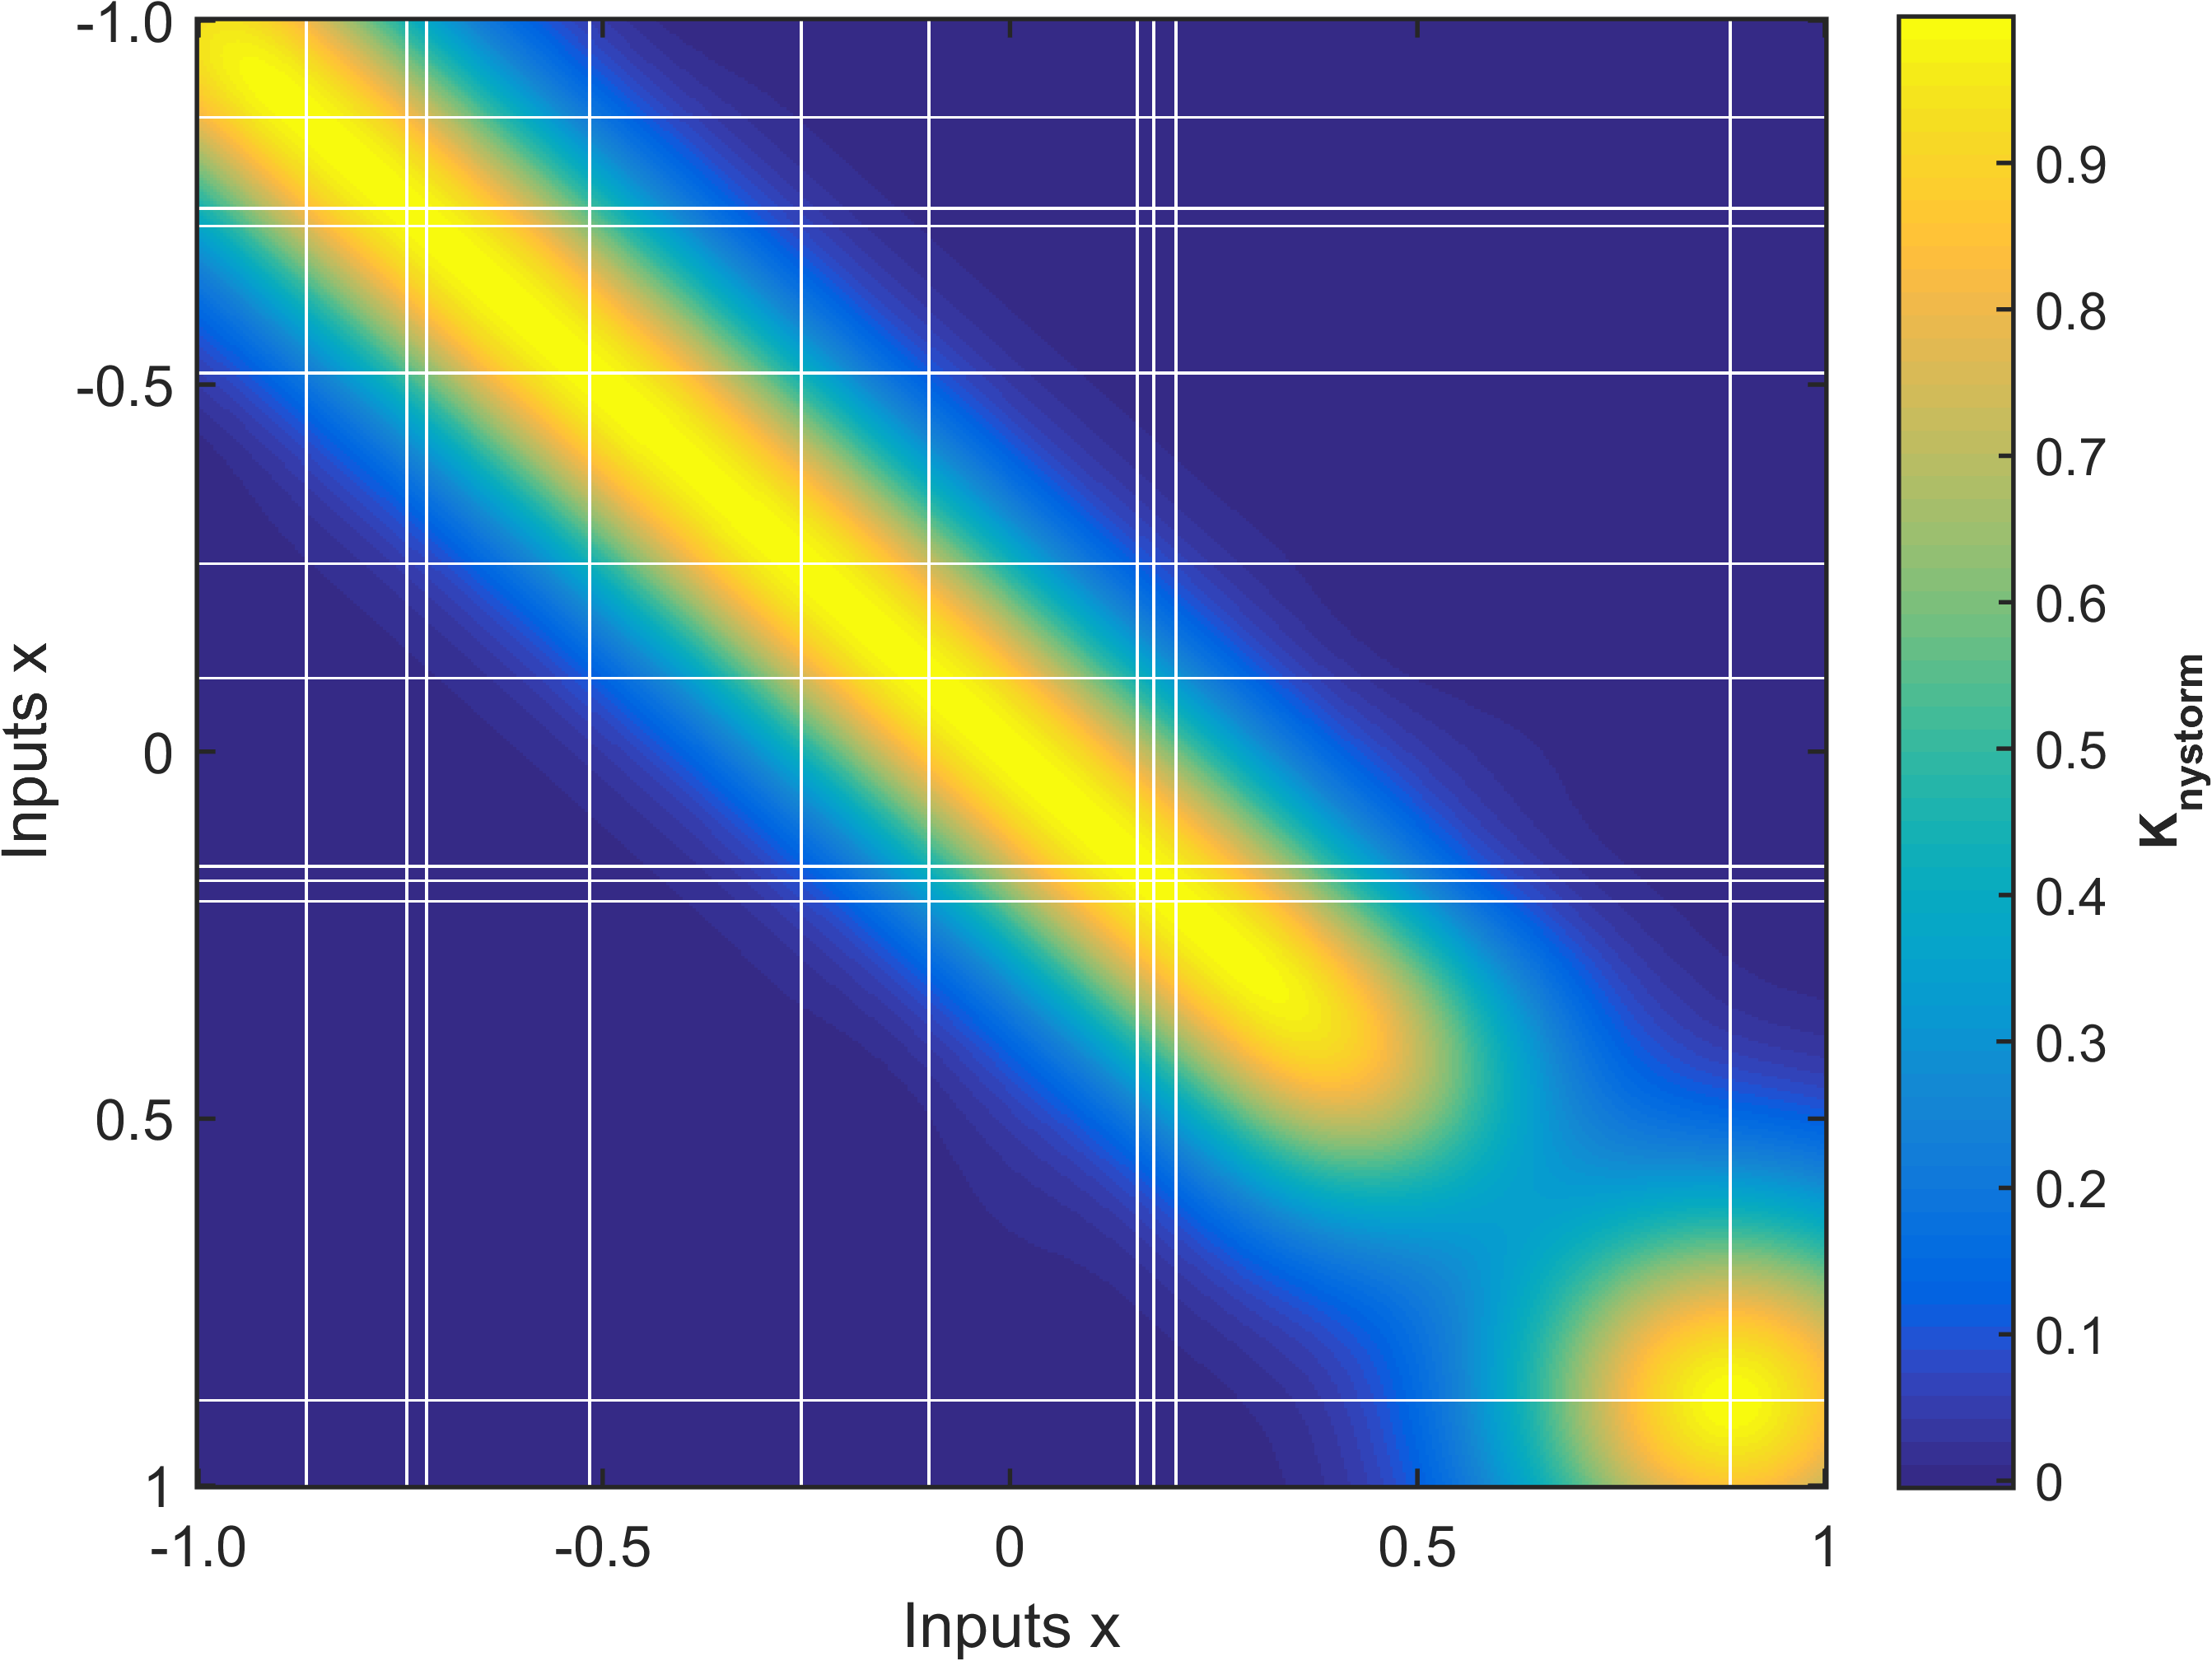
\includegraphics[width=0.45\textwidth]
        {images/nystormSEmatrix}
        \label{subFigNystormSEmatrix}
  }\quad
\subfigure[{Approximated Gram matrix using Nystr\"{o}m approximation for a Standard Exponential (SE) Kernel with \((\theta = [1, 0.2])\) (figure \ref{subFigcovSEmatrix_1}) at the input points \(X^{*} = \{[0:0.02:1]\}\). The white lines denote the location of inducing points, the inducing points are uniformly distributed. Notice the significant improvement in Gram matrix due to different inducing inputs}]
  {
        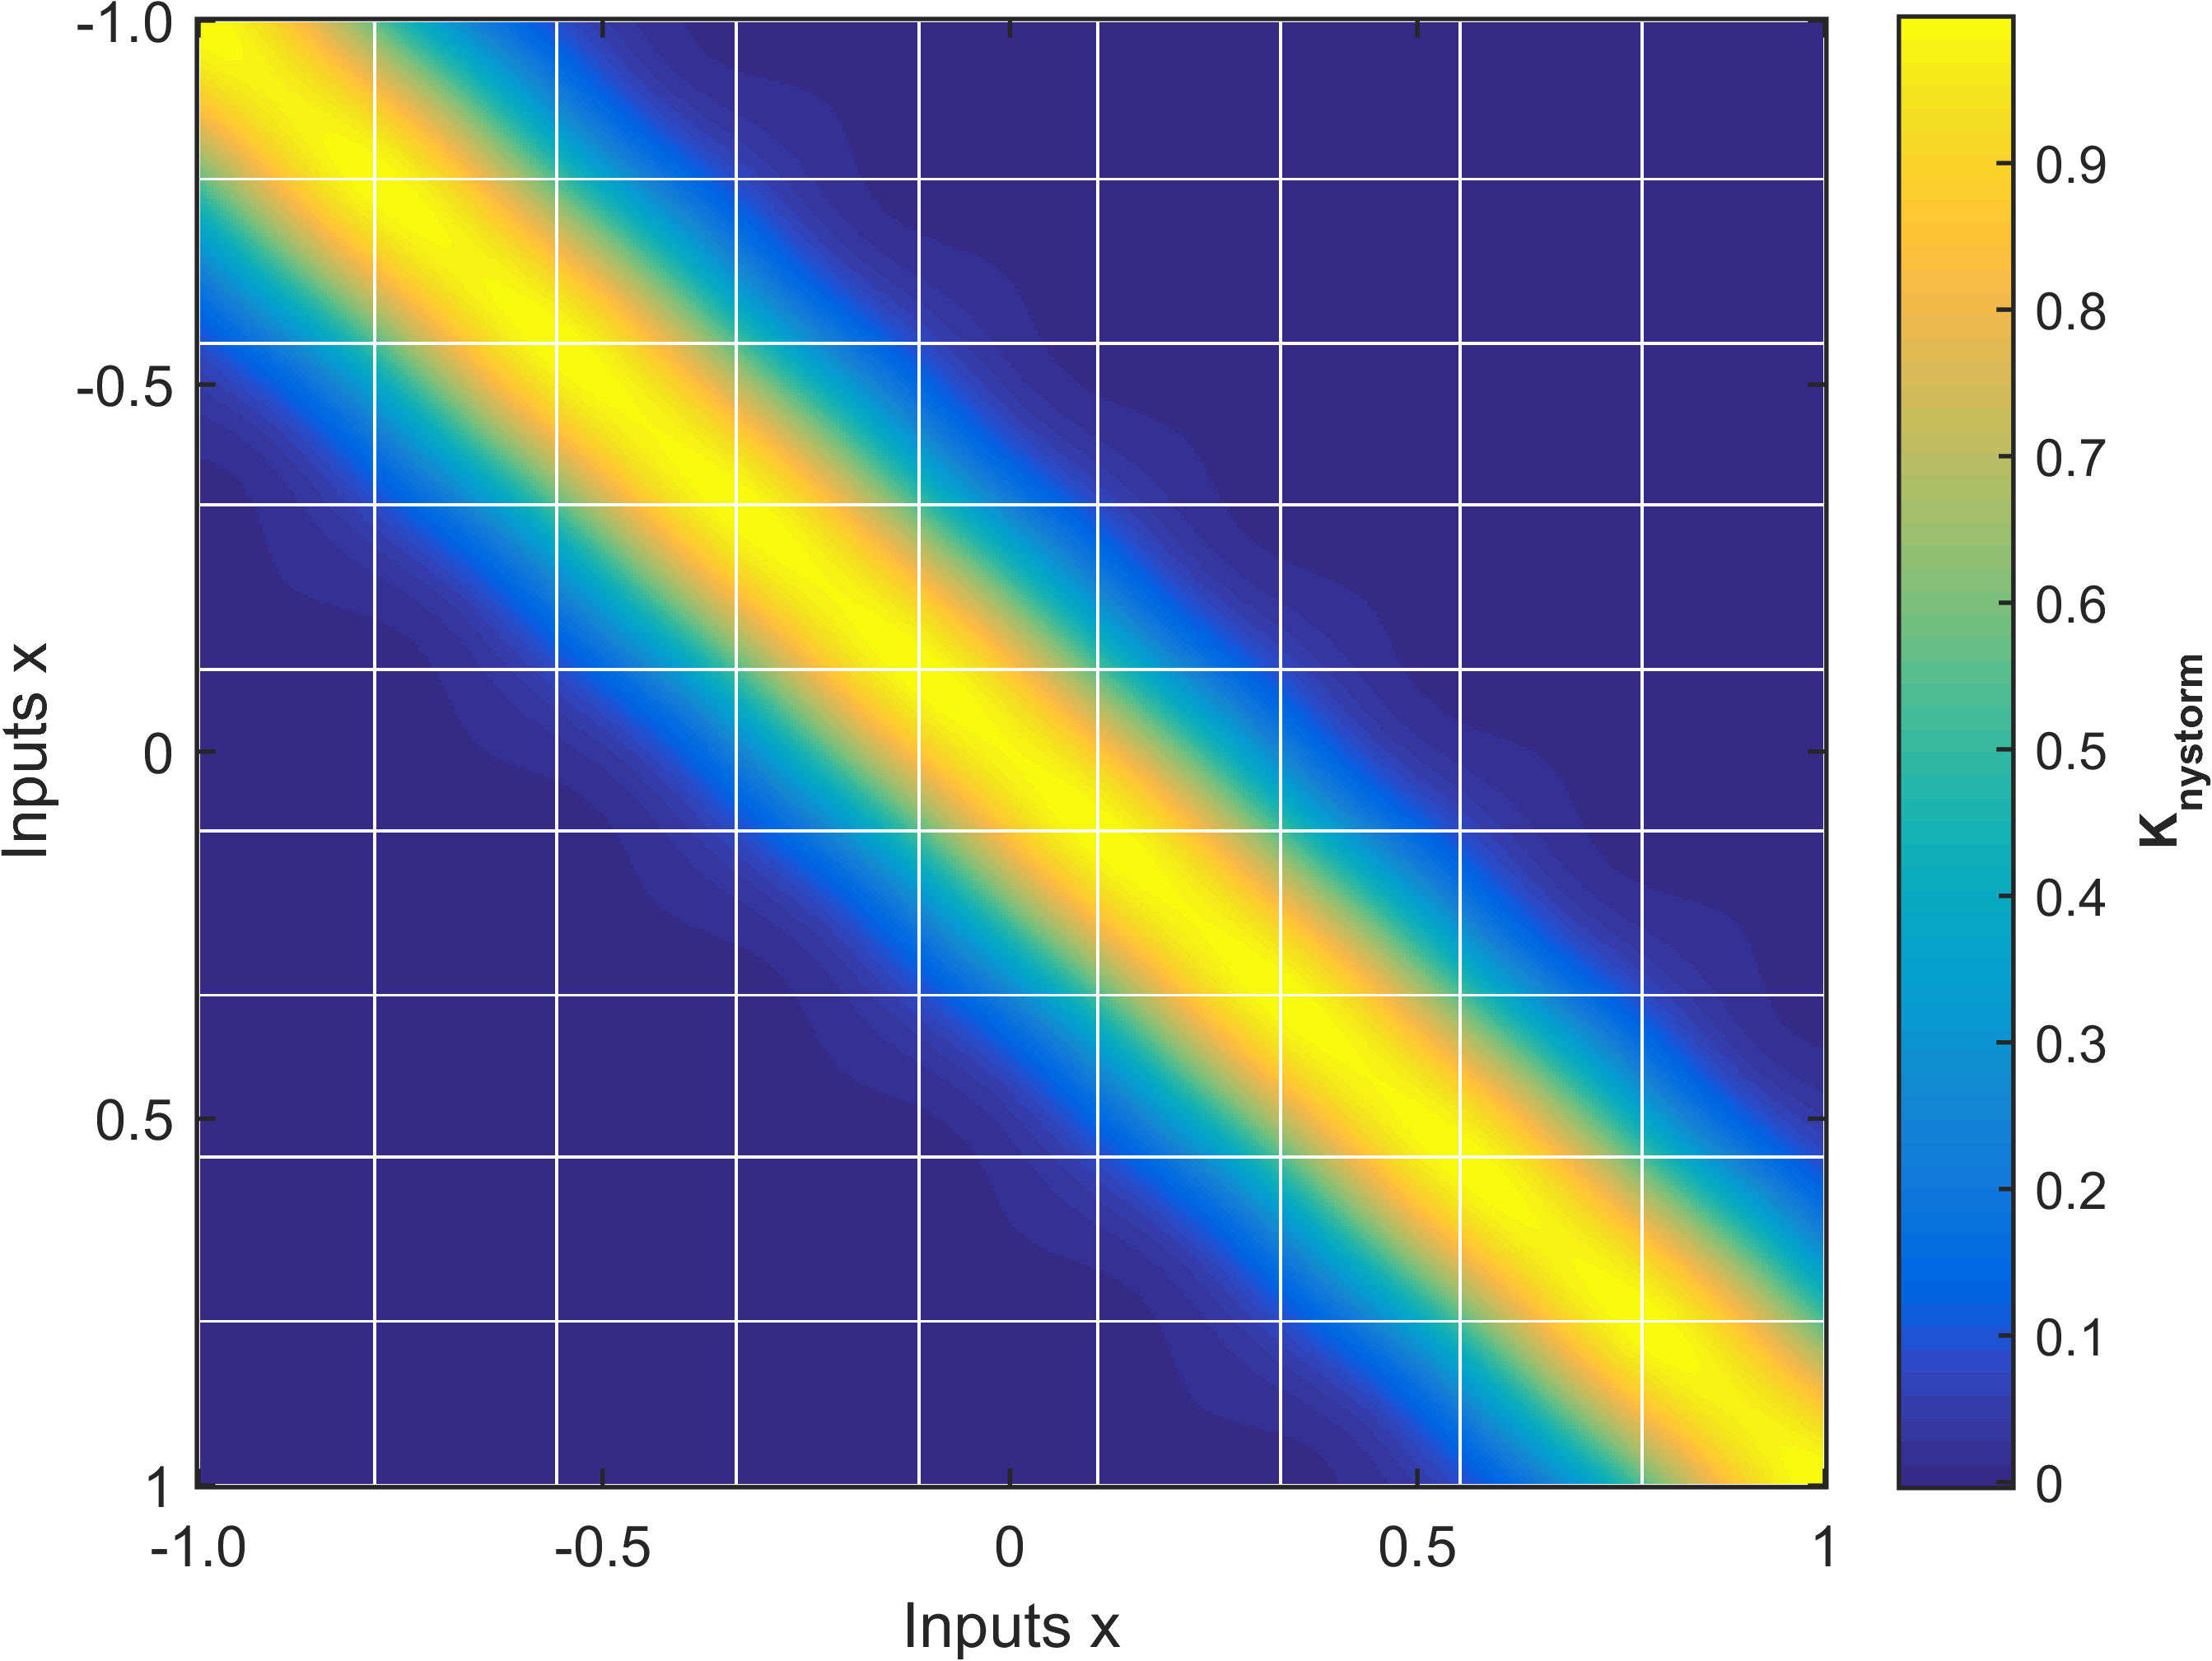
\includegraphics[width=0.45\textwidth]
        {images/nystormSEmatrixUniform}
        \label{subFignystormSEmatrixUniform}
  }\quad
  
       \caption{Approximate Gram matrix for a Standard Exponential kernel using Nystr\"{o}m approximation.}\label{figGPNystormGramMatrix}
\end{figure}

Later, \cite{Snelson06sparsegaussian} proposed the FITC approach which corrects the diagonal terms of the Gram matrix and improves the prediction capabilities (equation \ref{eqnSparseNystormGram}).

\begin{equation}\label{eqnSparseFITCGram}
K_{FITC}(X, X) = diag[K(X, X) - K_{nystorm}(X, X)] + K_{nystorm}(X, X)
\end{equation}

Note, calculating \(diag(K(X, X))\) is an \(\mathcal{O}\left ( N \right )\) operation and thus does not significantly impact the time taken. 


The posterior distribution for the approximate prior can be derived similarly as given in appendix \textbf{add appendix ref} and is a Gaussian. The predictive mean and predictive variance are written as equation \ref{eqNoisyNystormPredictiveMean} and equation \ref{eqNoisyNystormPredictiveCovariance}. Here, \(K_{approximate}(X, X')\) can be the approximated Gram matrix either from the Nystr\"{o}m approximation (equation \ref{eqnSparseNystormGram}) or the FITC approximation (equation \ref{eqnSparseFITCGram}). 
\begin{equation}\label{eqNoisyNystormPredictiveMean}
  \mathbf{E}[f_{approximate}(x_{*})] = K_{Xx_{*}}^{T}( K_{approximate}(X, X') + \sigma^{2}_{n}I)^{-1}Y
  \end{equation}
\begin{equation}\label{eqNoisyNystormPredictiveCovariance}
	Cov[f_{approximate}(x_{*})] = K_{x_{*}x_{*}} - K_{Xx_{*}}^{T}( K_{approximate}(X, X') + \sigma^{2}_{n}I )^{-1} K_{Xx_{*}}
  \end{equation}


By approximating the \(K(X, X)\) using the inducing points we have effectively changed the GP prior. This means that \(X^{m}\) have also become the hyper-parameters of our GP prior. Hence, we should fine-tune locations of \(X^{m}\) and the hyper-parameters \(\theta\) to obtain a good prediction of our data. The marginal likelihood for the approximate prior (equation \ref{equationApproximateML}) be written similarly as equation \ref{equationMarginalLikelihood}.

\begin{equation}\label{equationApproximateML}
    \Pr[Y(X) \mid X, X^{m}, \theta, \sigma_{n}] = \mathcal{N}(0 , K_{approximate}(X, X') + \sigma^{2}_{n}I)
\end{equation}


The maximization of the marginal likelihood in equation \ref{equationApproximateML} with respect to (\(X^{m}\); \(\theta\)), is prone to over-fitting especially when the number of inducing inputs is large. This means that if we keep on increasing the number of inducing points a time will come when we will tend to decrease the accuracy of our predictions on the test data set. The variational approximation (detailed next) approach overcomes this issue of over-fitting by adding a regularization term penalizing over-fitting.

\subsection{Variational Approximation}\label{subSecVariationalApprox} 
The variational approximation does not attempt to approximate the Gram matrix. Instead, it assumes a probability distribution \(q(f)\) of the true posterior distribution \(p(f \mid y)\) and minimizes the distance between the two \cite{Titsias09variationallearning}. 

The \(q(f)\) is written in terms of inducing points (\(X^{m}\)) and the KL divergence \(KL(q||p)\)\footnote{KL divergence is a measure of distance between two probability distributions} is minimized between the variational distribution \(q\) and true distribution \(p\). When we minimize the KL divergence we are making the assumed distribution closer to true distribution and hence improving the values of (\(X^{m}\)) and \(\theta \). This minimization of KL divergence is equivalently expressed as the maximization of the equation \ref{equationLowerBoundVarNLML}

\begin{equation}\label{equationLowerBoundVarNLML}
F_{V} = log(\mathcal{N}[0, \sigma_{n}^{2}I + K_{nystorm}(X, X)]) - \frac{1}{2\sigma_{n}^{2}}Tr(K_{XX} - K_{nystorm}(X, X))
\end{equation}

Notice, the similarity between equation \ref{equationLowerBoundVarNLML} and \ref{eqnSparseNystormGram}. The novelty of the above objective function is that it contains a regularization term: \(- \frac{1}{2\sigma ^{2}}Tr(K_{XX} - K_{nystorm}(X, X))\). Thus, \(F_{V}\) attempts to maximize the marginal likelihood as derived for Nystr\"{o}m approximation and simultaneously minimizes the trace. When the regularization term tends to zero \(K_{XX} - K_{nystorm}(X, X)\), which means that the inducing variables can exactly reproduce the full GP prediction. 

The posterior distribution for variational inference approximation is same as the one derived for Nystr\"{o}m approximation. The difference between Nystr\"{o}m approximation and variational approximation is the improvement in the evaluation parameter while optimizing \(X^{m}\) and \(\theta\). Due to the additional trace term variational inference reduces over-fitting.

\subsection{Experiments}\label{subsecNystromExperiments}
We here conduct experiments on a toy-data set to observe the accuracy of Nystr\"{o}m approximation for varying number and location of inducing points. The basic toolbox used for this paper is GPML provided with \cite{rasmussen2006gaussian} on MATLAB 2014b. All experiments were performed on an Intel quad-core processor with 4Gb RAM. 

10-fold Cross Validation (CV) will be used to assess the performance of the prediction. CV is a technique where the dataset is partitioned as the test set and training set. A model is learned using the training set and Root Mean Square Error (RMSE) is calculated between the prediction and test set as a measure of accuracy. In the 10-fold version of CV, the dataset will be randomly partitioned into 10 subsets containing an equal number of points. Of the 10 subsets, a single subset is retained as the test dataset, and the remaining 9 (10 - 1) subsets are used as training data. The cross-validation process is then repeated 10 times (the folds), with each of the k subsets used exactly once as the validation data.

The toy data set was generated at 1000 input points \(X = \{[-1:0.002:1]\}\) by sampling a random function from a GP\footnote{\((\Pr[Y \mid X, \theta, \sigma_{n}] = GP(0, K_{SE}(X, X', \theta = [1, 0.1]) + (0.3)^{2}I)\)} with zero mean, SE covariance function (\(\theta = [1, 0.1]\)) and noise \(\sigma_{n} = 0.3\). 

Figure \ref{predictionOfm10_242} is the prediction of the GP obtained after Nystr\"{o}m approximation using 10 inducing points. The solid black line defines the mean function, blue region defines 95\% confidence interval (2\(\sigma\)) distance away from the mean. The points denoted by `+' sign are initial locations of inducing points, while the points denoted by `*' sign are locations of inducing points after optimization. The points denoted by `.' are the test points for this fold of the 10-fold CV. 

Notice the inducing points, while initially randomly distributed are later uniformly distributed due to optimization of marginal likelihood. In this case, since the training points are randomly distributed, uniformly distributed inducing inputs are better approximations of the Gram matrix. In cases where training data set tends to be dense in one region and sparse in another region, lesser inducing points get allocated at the dense region and more get allocated at the sparse region. This happens because the information contained in a dense cluster of data-points can be approximated by a fewer data points (points in a neighbourhood are similar (section \ref{subSecCH2Covariance}) \cite{Snelson06sparsegaussian}.

Figure \ref{boxPlotsOfPerformance_242} are 10-fold RMSE box-plots for varying number of inducing points. The box-plots in red are cases when only the hyper-parameters were optimized while inducing inputs were distributed randomly.The box-plots in blue are the cases when both locations of inducing points and hyper-parameters are optimized. The accuracy of prediction improves with increasing number of inducing points. Accuracy is generally better when both locations of inducing points and hyper-parameters are optimized. Note, the noise in the generated toy-data is \(\sigma_{n}=0.3\), hence \(0.3\) is the best achievable RMSE value. Models constructed when optimizing both \(\theta, X^{m}\) reach this RMSE limit for \(M = 20\). After \(M=50\) accuracy is similar for both the optimization routines. As a thumb rule if \(M = \frac{N}{10}\) then randomly distributing the inducing points and optimizing \(\theta\) will be sufficient to give a good prediction \cite{cao2013efficient}. 

\begin{figure}[!ht]
  \centering
    \subfigure[{Posterior between a Nystorm approximated SE prior with 10 inducing inputs and training data. The solid black line defines the mean function, blue region defines 95\% confidence interval (2\(\sigma\)) distance away from the mean. The points denoted by `+' sign are initial locations of inducing points, while the points denoted by `*' sign are locations of inducing points after optimization.}]
  {
        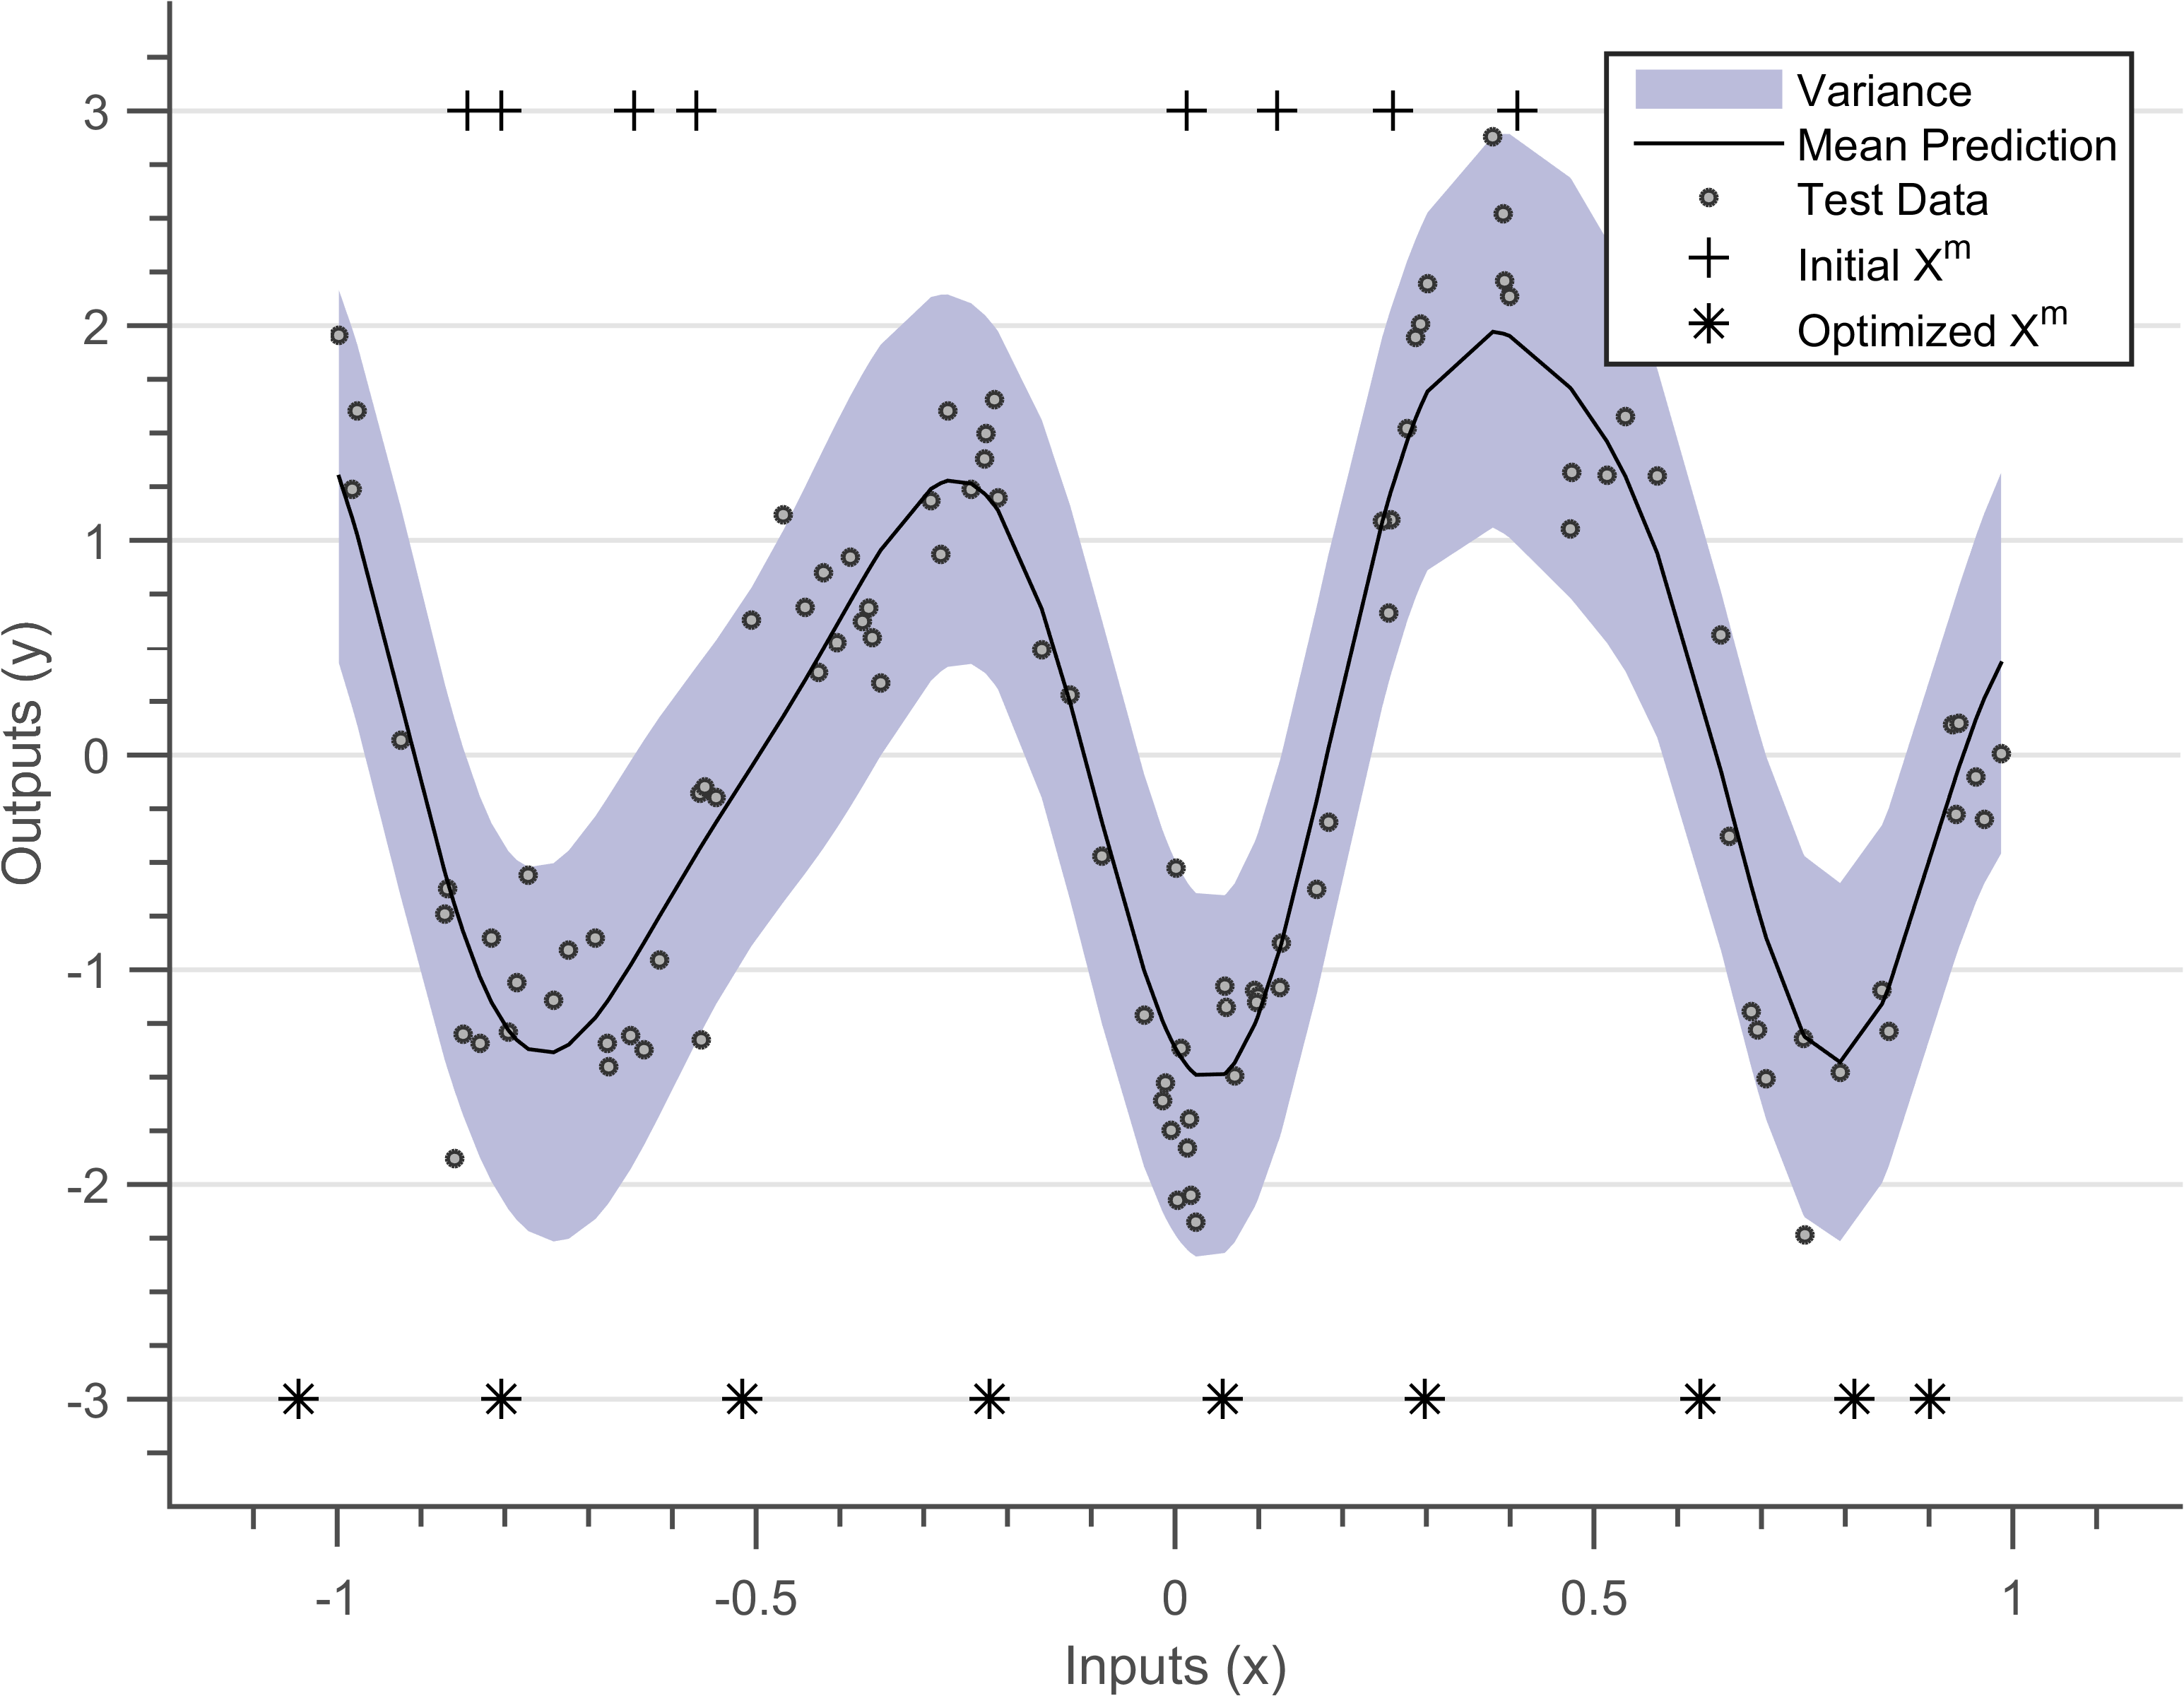
\includegraphics[width=0.45\textwidth]
        {images/predictionOfm10_242}
        \label{predictionOfm10_242}
  }\quad
\subfigure[{10-fold RMSE box-plots for varying number of inducing points. The box-plots in red are cases when only the hyper-parameters \(\theta\) were optimized while inducing inputs were distributed randomly. The box-plots in blue are the cases when both locations of inducing points \(X^{m}\) and hyper-parameters \(\theta\) are optimized. }]
  {
        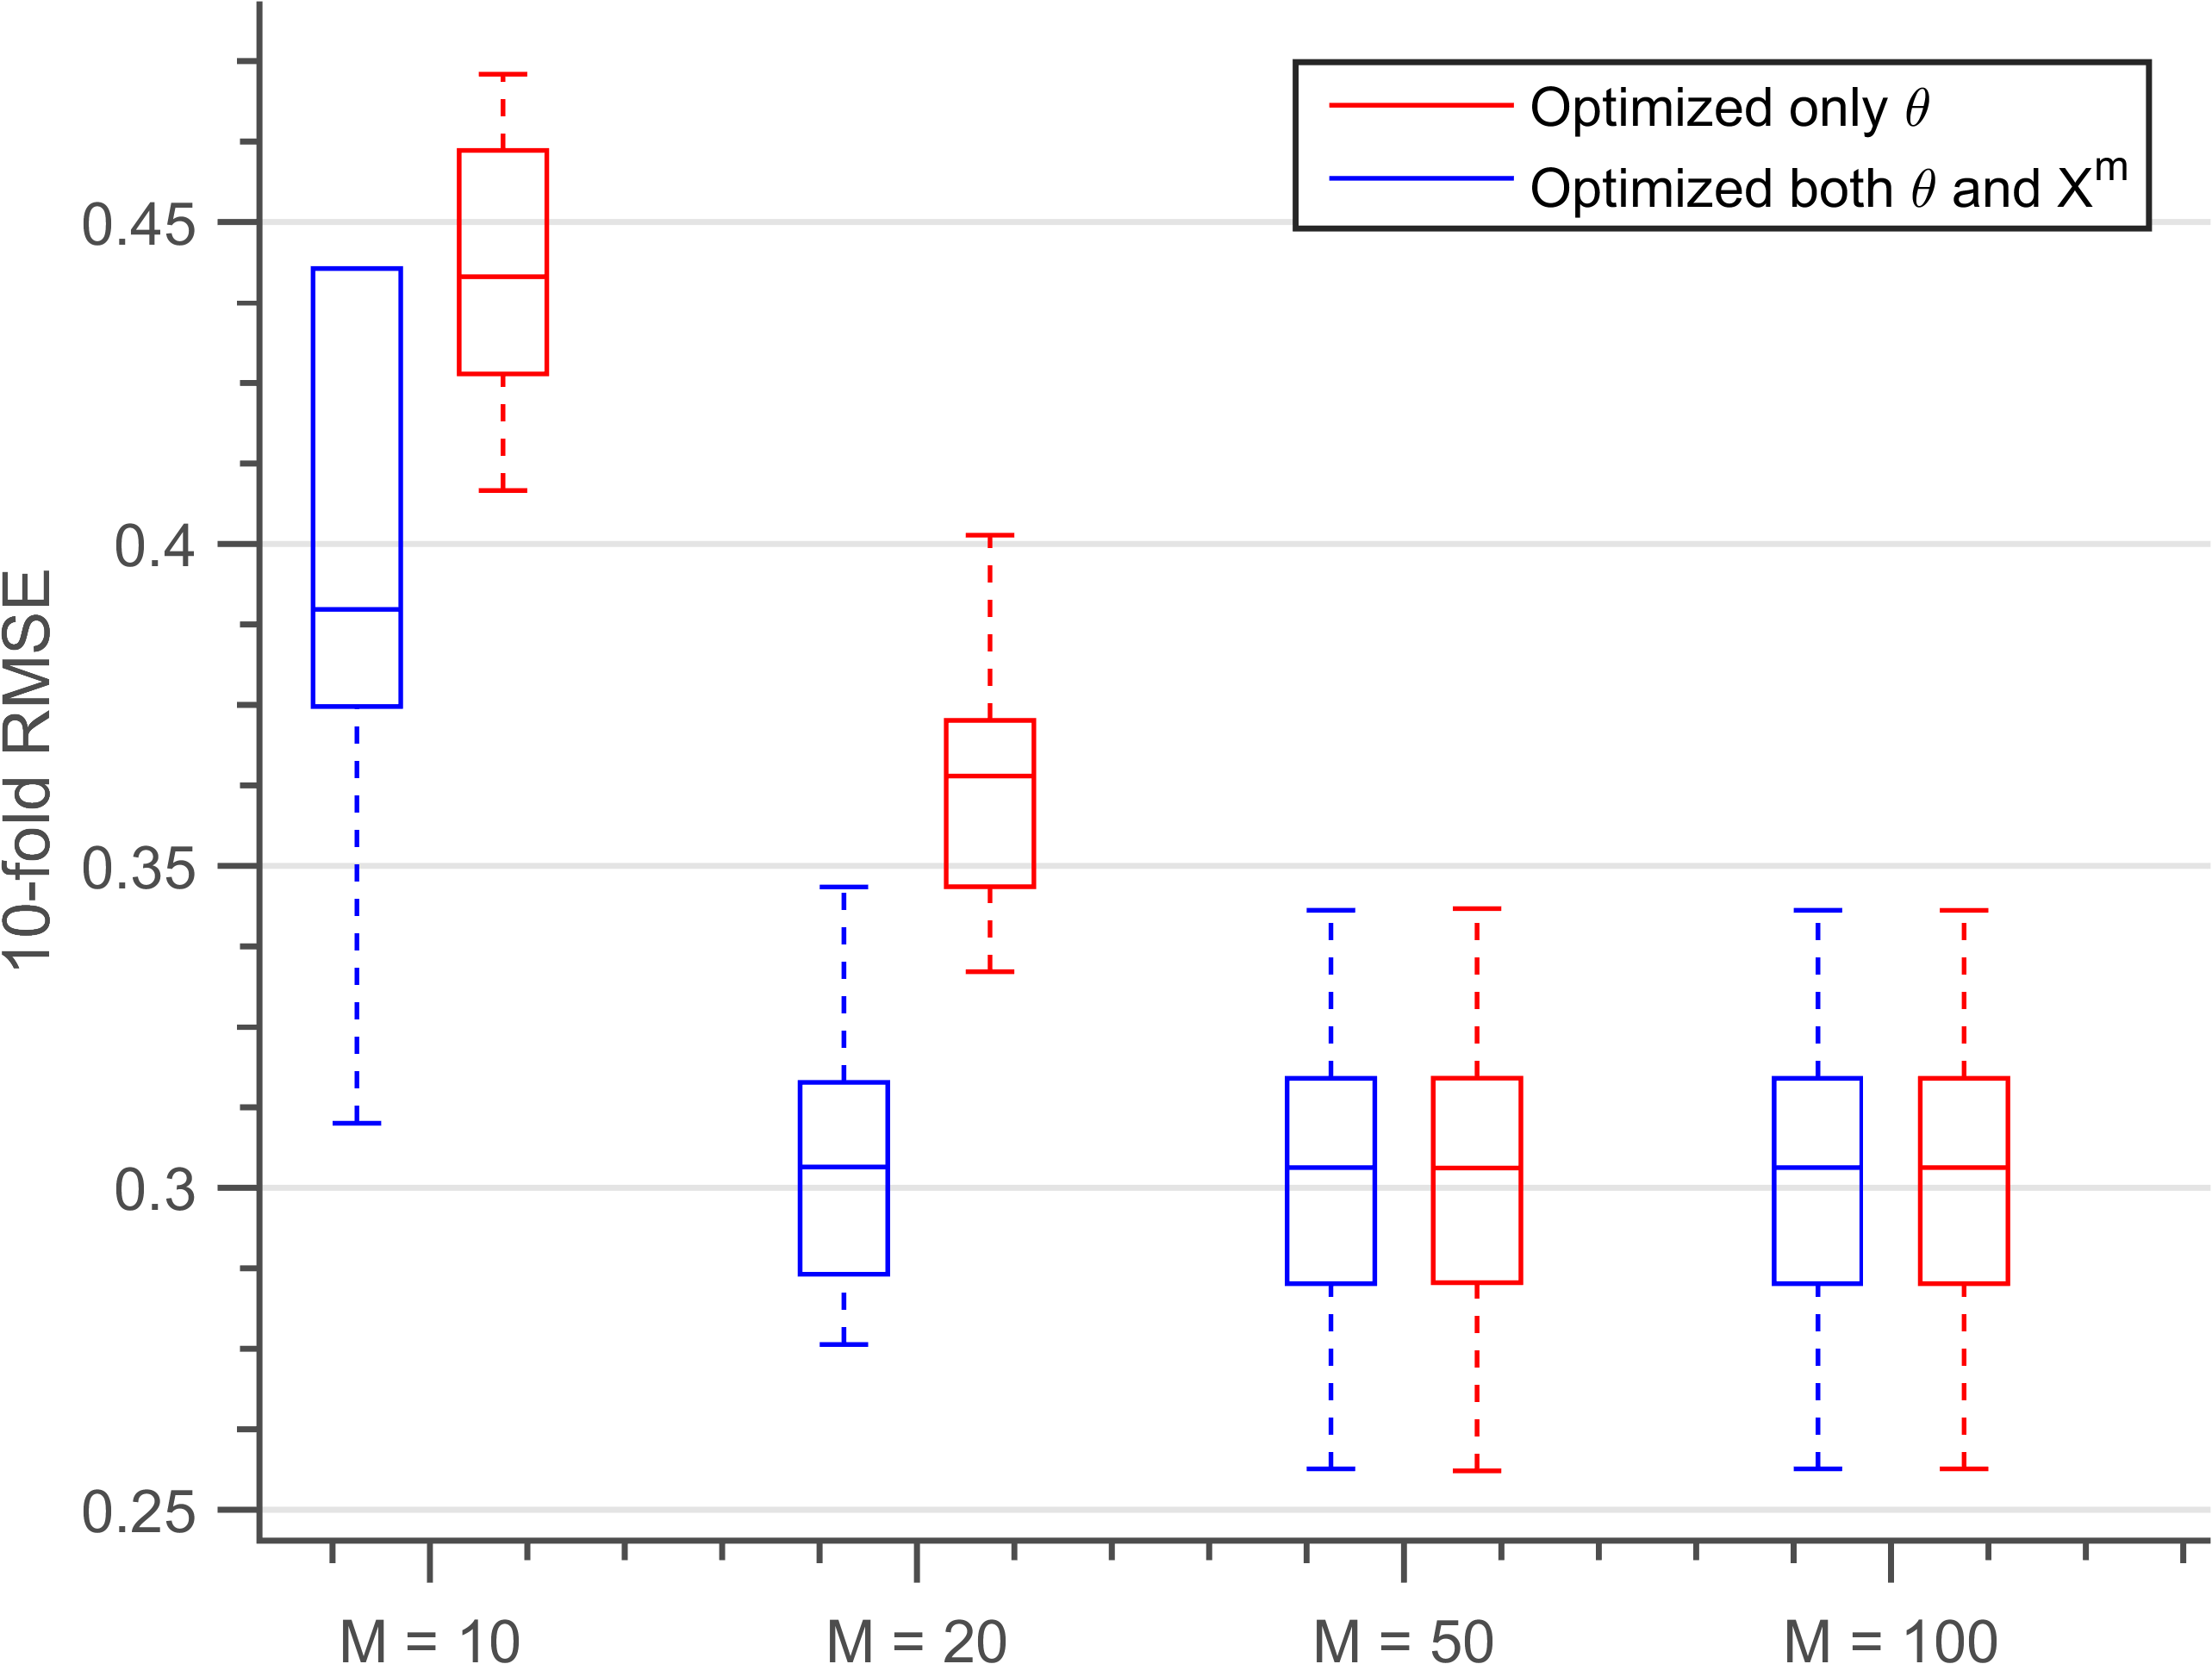
\includegraphics[width=0.45\textwidth]
        {images/boxPlotsOfPerformance_242}
        \label{boxPlotsOfPerformance_242}
  }\quad
  
       \caption{Results of Nystr\"{o}m Approximation on a toy-data set of size \(N=1000\) }\label{figGPPredictionNystorm}
\end{figure}

Global low-rank approximations are best suited for the case of spread out Gram matrices (example high length-scale SE priors). We have seen three types of low-rank approximation algorithms in this section. While Nystr\"{o}m and FITC approximations are the simplest method to approximate Gram matrix, finding optimal locations of the inducing points can often lead to over-fitting. We then, look at variational approximation procedure which adds a regularization term while finding inducing points thereby penalizing over-fitting. The lower computational cost due to sparse approximations, scales sparse GPs to the training set of sizes \(N \sim \mathcal{O}(5 \times 10^5)\). \cite{Gal2014Distributed} propose a distributed architecture for scaling variational sparse GPs. In the next section we look at how to approximate Gram matrices using mixture of experts, this enables us to massively scale GPs to sizes \(N > \mathcal{O}(10^6)\) by exploiting distributed architecture.

\section{Distributed Gaussian Process}\label{secDgp}
In the year 2006 Netflix prize was launched, teams from all over the world competed in the competition to make the best video recommendation algorithm. As the competition progressed teams figured out that performance increases upon combining algorithms developed by multiple teams. The winner and the runner-up were stacked learners of over 100 algorithms. Creating model ensembles (also called mixture of experts) is now a standard practice in many learning competitions \cite{bauer1998empirical}. 

Mixture of experts methods in GPs use bagging, where subsets of data are generated, individual GPs are trained on these subsets and their results are finally combined \cite{chen2009bagging}. If the data set is partitioned  into \(N_{experts}\) subsets such as $\mathcal{D}^{(i)} = {X^{(i)}, Y^{(i)}}, i \in 1, \ldots N_{experts}$. Each subset of data learns an individual GP model, which can be combined together to give final predictions . Due to individual learning choosing hyper-parameters and calculating prediction become easily parallel-able and indifferent to the computational infrastructure. 

Initially, this mixture of local models was used to highlight local features in the data \cite{rasmussen2002infinite}. \cite{ng2014hierarchical} propose to use the mixture of experts methodology to speed up prediction in a Gaussian Process. Instead of learning a different GP for each subset, we tie all the different experts using one single set of hyperparameters. This is equivalent to assuming one single GP for the whole data-set such that there is no correlation across experts, i.e. the experts are independent of each other. This tying of experts greatly reduces the number of hyper-parameters to optimize, acts as a regularization and inhibits over-fitting. Equation \ref{distributedGPPrior} denotes an independent GP prior for each expert \(\mathcal{D}^{(i)}\) such that the hyper-parameters \(\theta\) and \(\sigma_{n}\) are same for all experts.

\begin{equation}\label{distributedGPPrior}
    \Pr[y^{(i)} \mid x^{(i)}, \theta, \sigma_{n}] = GP(0, K(x^{(i)}, x^{(i)'}, \theta) + \sigma^{2}_{n}I) 
\end{equation}

Figure \ref{subFigdistributedKernelRandomExperts} is an approximate Gram matrix using distributed GP approximation for a Standard Exponential (SE) Kernel with \((\theta = [1, 0.2])\) (figure \ref{subFigcovSEmatrix_1}) at the input points \(X^{*} = \{[0:0.02:1]\}\). 5 experts each having 100 points are chosen, points in the experts are distributed randomly, this gives the approximate Gram matrix scattered shape. Figure \ref{subFigDistributedKernel} is an approximate Gram matrix using distributed GP approximation of the matrix in figure \ref{subFigcovSEmatrix_1} and uniformly distributed experts. 5 experts each having 100 points are chosen, The first expert has first set of 100 points, the second expert has the second set of 100 points and so on. The Gram matrix with randomly chosen experts has a more global nature but lacks many high variance regions. The Gram matrix for uniformly chosen experts retains more local features. Inversion of this Gram matrix is an operation of complexity \(\mathcal{O}(N_{experts}P^{3})\), where \(P\) is the number of points in an expert.

\begin{figure}[!ht]
  \centering
    \subfigure[{Approximated Gram matrix using distributed GP approximation for a Standard Exponential (SE) Kernel with \((\theta = [1, 0.2])\) (figure \ref{subFigcovSEmatrix_1}) at the input points \(X^{*} = \{[0:0.02:1]\}\). Points in the experts are distributed randomly, this gives the approximate Gram matrix scattered shape.}]
  {
        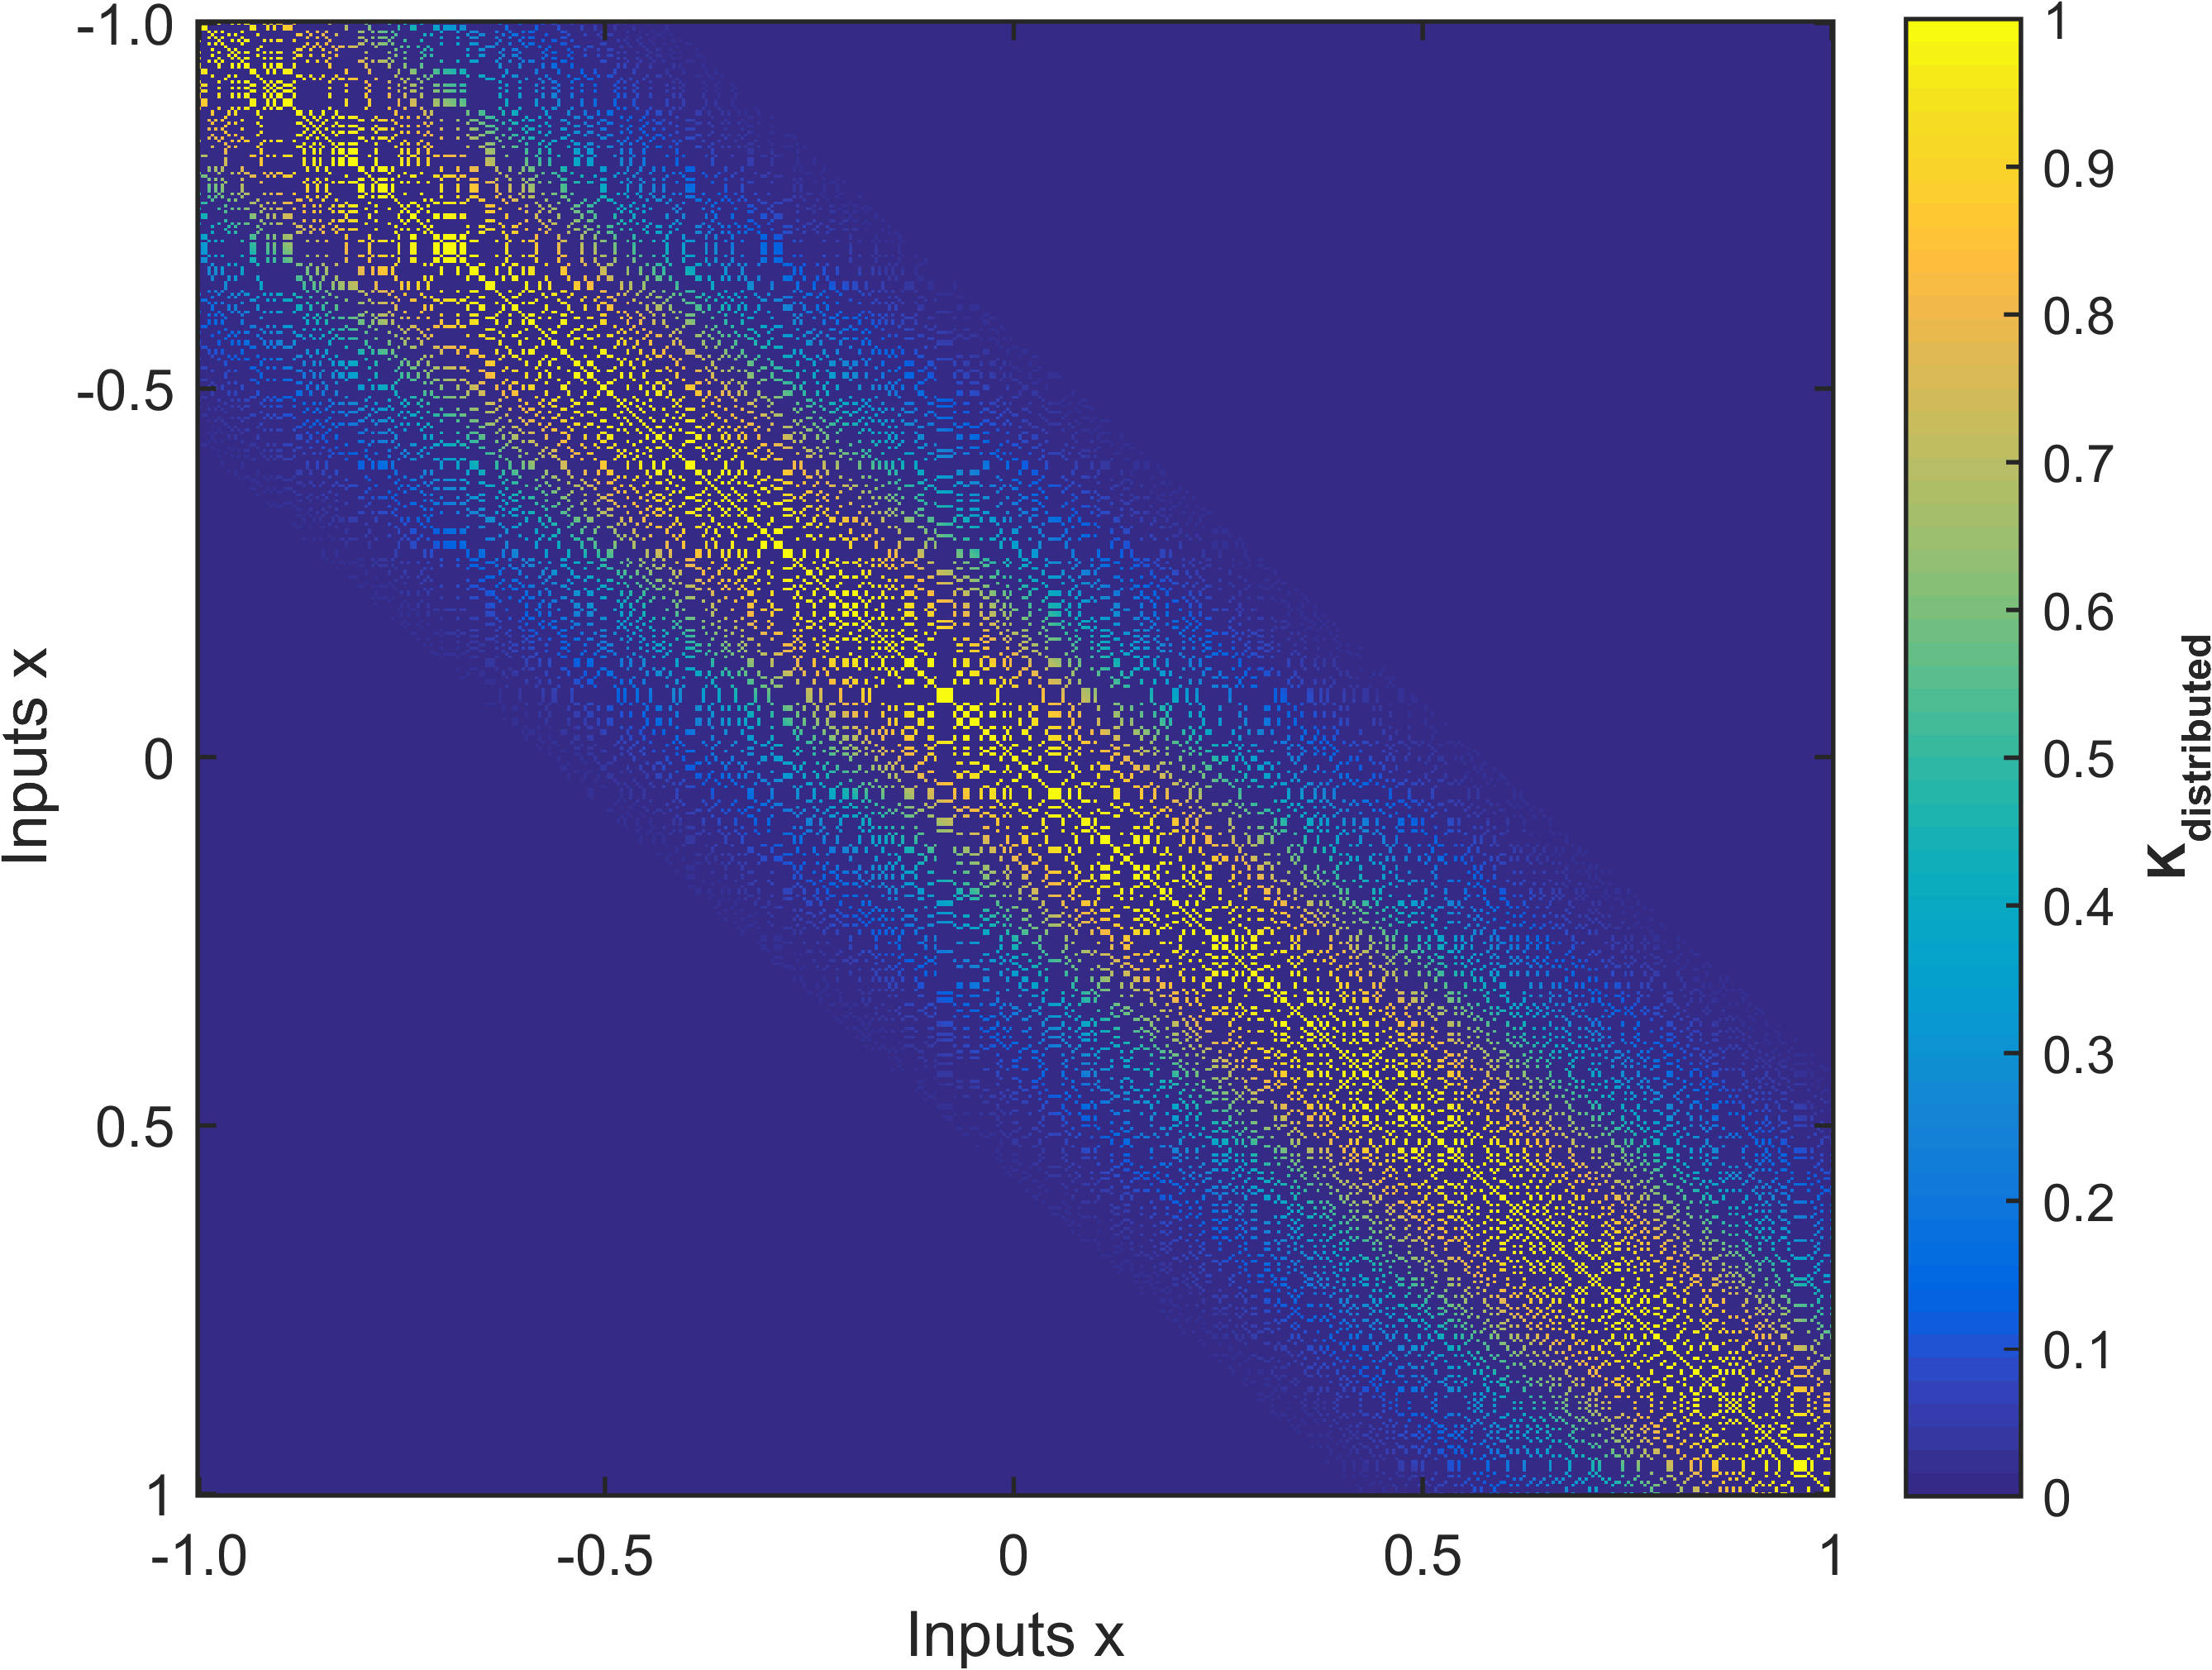
\includegraphics[width=0.45\textwidth]
        {images/distributedKernelRandomExperts}
        \label{subFigdistributedKernelRandomExperts}
  }\quad
\subfigure[{Approximated Gram matrix using distributed GP approximation for a Standard Exponential (SE) Kernel with \((\theta = [1, 0.2])\) (figure \ref{subFigcovSEmatrix_1}) at the input points \(X^{*} = \{[0:0.02:1]\}\). Points in the experts are distributed uniformly. We can observe that covariance across experts goes to zero.}]
  {
        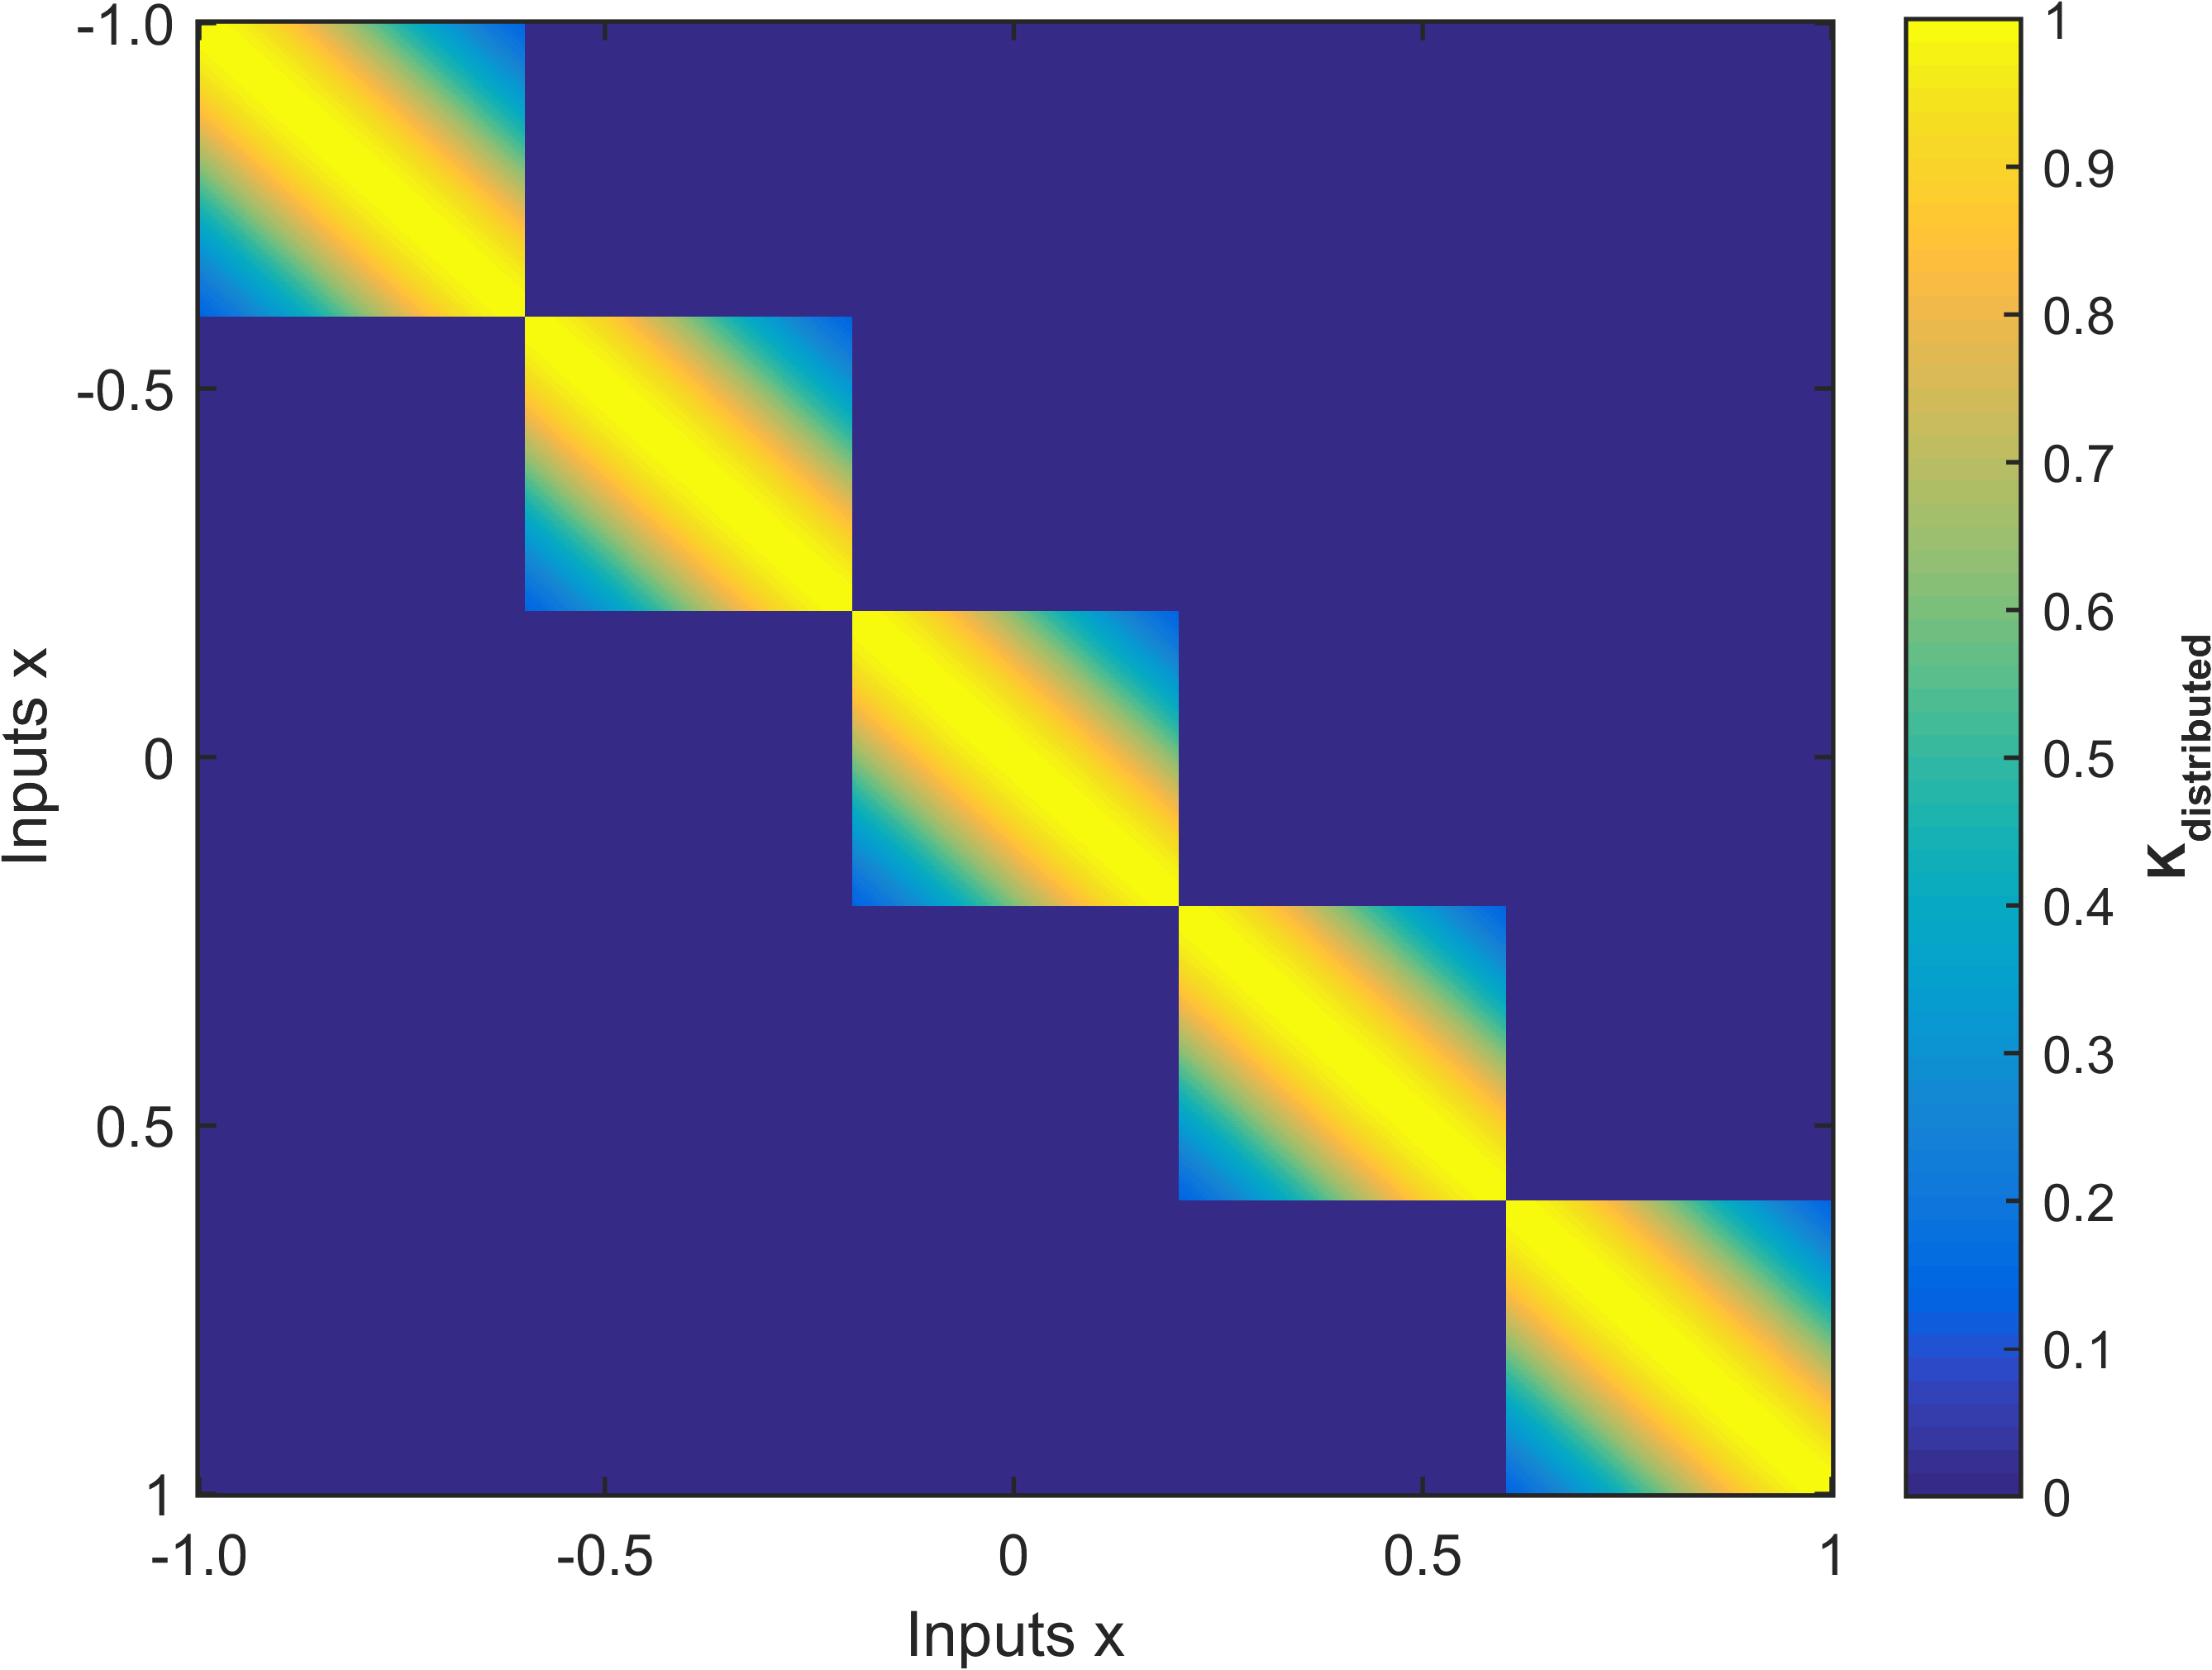
\includegraphics[width=0.45\textwidth]
        {images/distributedKernel}
        \label{subFigDistributedKernel}
  }\quad
  
       \caption{Approximate Gram matrix for a Standard Exponential kernel using mixture of experts.}\label{figGPApproximateDGPMatrix}
\end{figure}

Since the experts are independent of each other, we can construct a posterior distribution for each expert (equations \ref{eqPredictiveMeanIndividualExpert} and \ref{eqPredictiveCovarianceIndividualExpert}). In the following equations \(m^{(i)}(x_{*})\) and \(\sigma^{(i)}(x_{*})\) are the mean and covariance predictions from expert \(i\) at point \(x_{*}\).  

\begin{equation}\label{eqPredictiveMeanIndividualExpert}
  m^{(i)}(y(x_{*})) = K_{x^{(i)}x_{*}}^{T}( K_{x^{(i)}, x^{(i)'}} + \sigma^{2}_{n}I)^{-1}y^{(i)}
  \end{equation}
\begin{equation}\label{eqPredictiveCovarianceIndividualExpert}
	\sigma^{(i)}(y(x_{*})) = K_{x_{*}x_{*}} - K_{x^{(i)}x_{*}}^{T}( K_{x^{(i)}, x^{(i)'}} + \sigma^{2}_{n}I )^{-1} K_{x^{(i)}x_{*}}
  \end{equation}

\subsection{Combining experts}\label{subSecCombiningExperts}
There exist several methods in the literature on how to combine these individual posterior predictions of the experts to give the final posterior distribution. The Product of Experts model uses the independence assumption between experts and multiplies the individual posterior distribution\footnote{\(\Pr[y(x_{*}) \mid x_{*}, \mathcal{D}, \theta] \propto \prod \Pr[y^{(i)} \mid x^{(i)}, \mathcal{D}^{(i)}, \theta]\)}, but these predictions tend to be overconfident. Another method called the generalized Product of Experts (gPOE) assigns a participation factor to each expert based on the amount of uncertainty in prediction (more confident experts have higher say in prediction)\cite{cao2014generalized}. The Bayesian Committee Machine (BCM) imposes the independence assumption between each expert pair using Bayes Rule, but can result in bad predictions when leaving data regime \cite{tresp2000bayesian}. 

This thesis will use robust Bayesian Committee Machine (rBCM) model to combine the posterior distributions of experts \cite{deisenroth2015distributed}. The rBCM model is an amalgamation of all the above three mentioned methods, it combines the confidence weighting parameter of gPOE with the Bayesian formulation in BCM technique to generate the following posterior distributions.

\begin{equation}\label{eqCovarianceDGP}
    Cov(y(x_{*}))^{^-2} = \sum_{i} \beta_{i}\sigma_{(i)}^{-2} + (1- \sum_{i} \beta_{i})(K_{x_{*}x_{*}})^{-2}
\end{equation}
\begin{equation}\label{eqMeanDGP}
    m(y(x_{*})) = (Cov(y(x_{*})))^{-2}\sum_{i} \beta_{i}(\sigma^{(i)})^{-2}m^{(i)}(x_{*})
\end{equation}

\(K_{x_{*}x_{*}}\) is the auto-covariance of the prior at prediction point \(x_{*}\). \(\beta_{k}\) determines the influence of experts on the final predictions \cite{cao2014generalized} and is given as \(\beta_{i} = \frac{1}{2}(\log K_{x_{*}x_{*}}^{2} - \log(\sigma^{(i)})^{2})\). Experts which are very confident of their predictions at \(x_{*}\) will tend to have low \(\sigma^{(i)}\) thereby leading to a higher influence factor \(\beta_{i}\).

Due to the independence assumption, the marginal likelihood can be written as a sum of individual likelihoods and then can be optimized to find the best-fit hyperparameters. By approximating the \(K(X, X)\) in terms of \(\mathcal{D}^{(i)}\) and \(N_{experts}\) we have again changed the GP prior. This means that the number of experts \(N_{experts}\) and clustering of points in individual experts also impact the prediction capabilities of GP. The below equation \ref{eqDGPNLML} describes the formulation for marginal likelihood. 

\begin{align}\label{eqDGPNLML}
    \log \Pr[y \mid X, \mathcal{D}, \theta] \approx \sum_{k=1}^{N_{experts}} \log \Pr[y^{(i)}\mid X^{(i)}, \theta]
 \end{align}

Maximizing the above log-marginal likelihood will give the optimal values of hyper-parameters. Points in the experts can be distributed either randomly or using a clustering scheme (eg. k-means clustering\footnote{k-means algorithm clusters close by points in one cluster. The notion of closeness is defined by some measure of distance}) for stationary kernels\footnote{stationary kernels are only a function of d = |x-x'|} k-means clustering should be preferred. The k-means algorithm clusters points based on a measure of distance, points in separate clusters are far away from each other when compared to points in the same cluster. This means that the covariance (for stationary kernels) between separate clusters is significantly lower when compared to points in same cluster. Hence, the cross-covariance across separate clusters can be more easily assumed to be zero.

\subsection{Experiments}\label{subSecDistributedExperiments}
We again conduct experiments on a toy-data set, this time to observe the accuracy of distributed GP approximation for varying number of experts. 

Again the 10-fold Cross Validation (CV) will be used to assess the performance of the prediction. The same toy-data set as used in section \ref{subsecNystromExperiments} was used to perform the experiments in this section (1000 data-points from \(\Pr[y \mid X, \theta, \sigma_{n}] = GP(0, K_{SE}(X, X', \theta = [1, 0.1]) + (0.3)^{2}I)\).

Figure \ref{predictionOfm10_243} is the prediction of the GP obtained after distributed approximation using 9 experts and k-means clustering. The solid black line defines the mean function, blue region defines 95\% confidence interval (2\(\sigma\)) distance away from the mean. The colored points in the points denoted by `*' at the bottom show how different points are distributed across experts, similar colored points belong to one expert. The data denoted by `.' is the test data for one fold of the 10-fold CV. 

The points across experts are uniformly distributed, as can be observed by the coloring scheme. Since the training points are almost uniformly distributed, the k-means algorithm will cluster the points uniformly. Actually, the training and test set used in figures \ref{predictionOfm10_243} and \ref{predictionOfm10_242} are same. Notice how Nystr\"{o}m approximation has a global smooth shape while the distributed GP approximation retains the local features of the data set. 

Figure \ref{boxPlotsOfPerformance_243} are 10-fold RMSE box-plots for different number of \(P\). The box-plots in red are cases when the points are distributed using k-means clustering. The box-plots in blue are the cases when points are distributed randomly. The accuracy of prediction improves with increasing number of points in an expert. Note, the noise in the generated toy-data is \(\sigma_{n}=0.3\), hence \(0.3\) is the best achievable RMSE value. Accuracy is slightly better when experts are distributed using k-means clustering, both being very close to the \(0.3\) RMSE limit. As a thumb-rule setting \(P = N/10\) and optimizing the hyper-parameters (\(\theta\)) is a good enough approximation. 


\begin{figure}[!ht]
  \centering
    \subfigure[{Prediction of the GP obtained after distributed approximation using 9 experts and k-means clustering. The solid black line defines the mean function, blue region defines 95\% confidence interval (2\(\sigma\)) distance away from the mean. The colored points in the points denoted by `*' at the bottom show how different points are distributed across experts, similar colored points belong to one expert. The data denoted by `.' is the test data for one fold of the 10-fold CV. }]
  {
        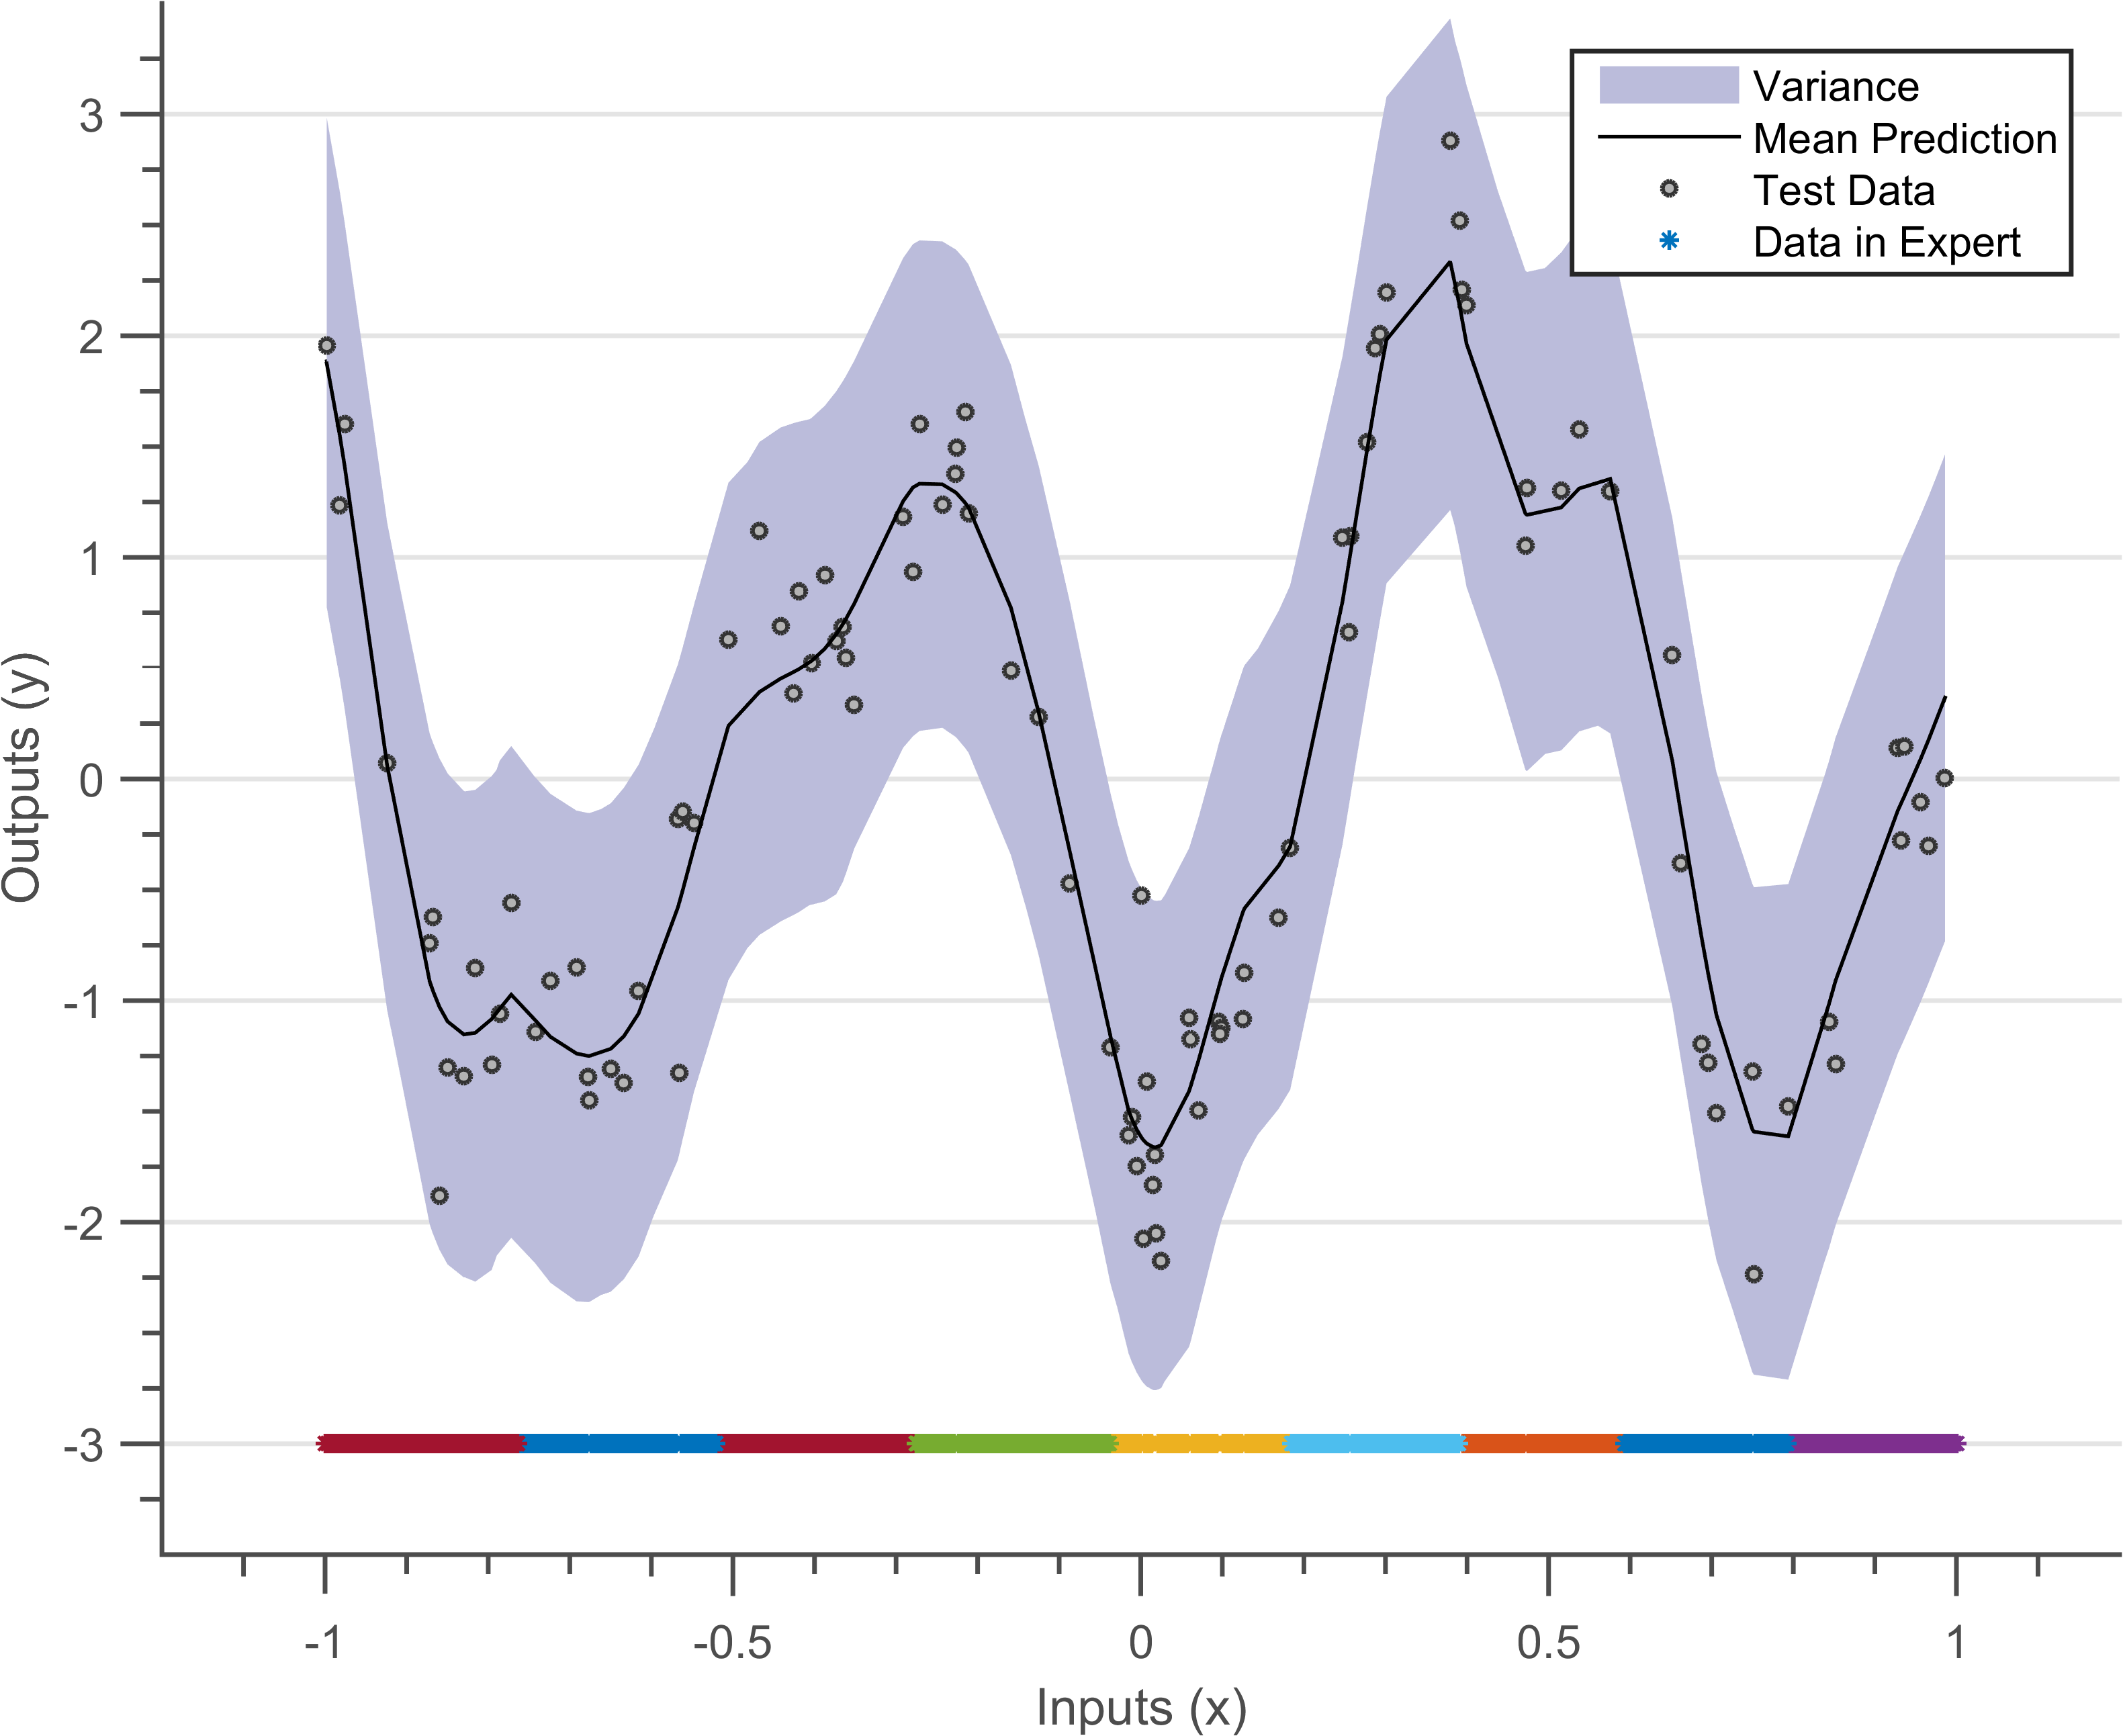
\includegraphics[width=0.45\textwidth]
        {images/predictionOfm10_243}
        \label{predictionOfm10_243}
  }\quad
\subfigure[{10-fold RMSE box-plots for different number of points across. The box-plots in red are cases when only the hyper-parameters when the points are distributed using k-means clustering. The box-plots in blue are the cases when points are distributed randomly. The accuracy of prediction improves with increasing number of points in an expert}]
  {
        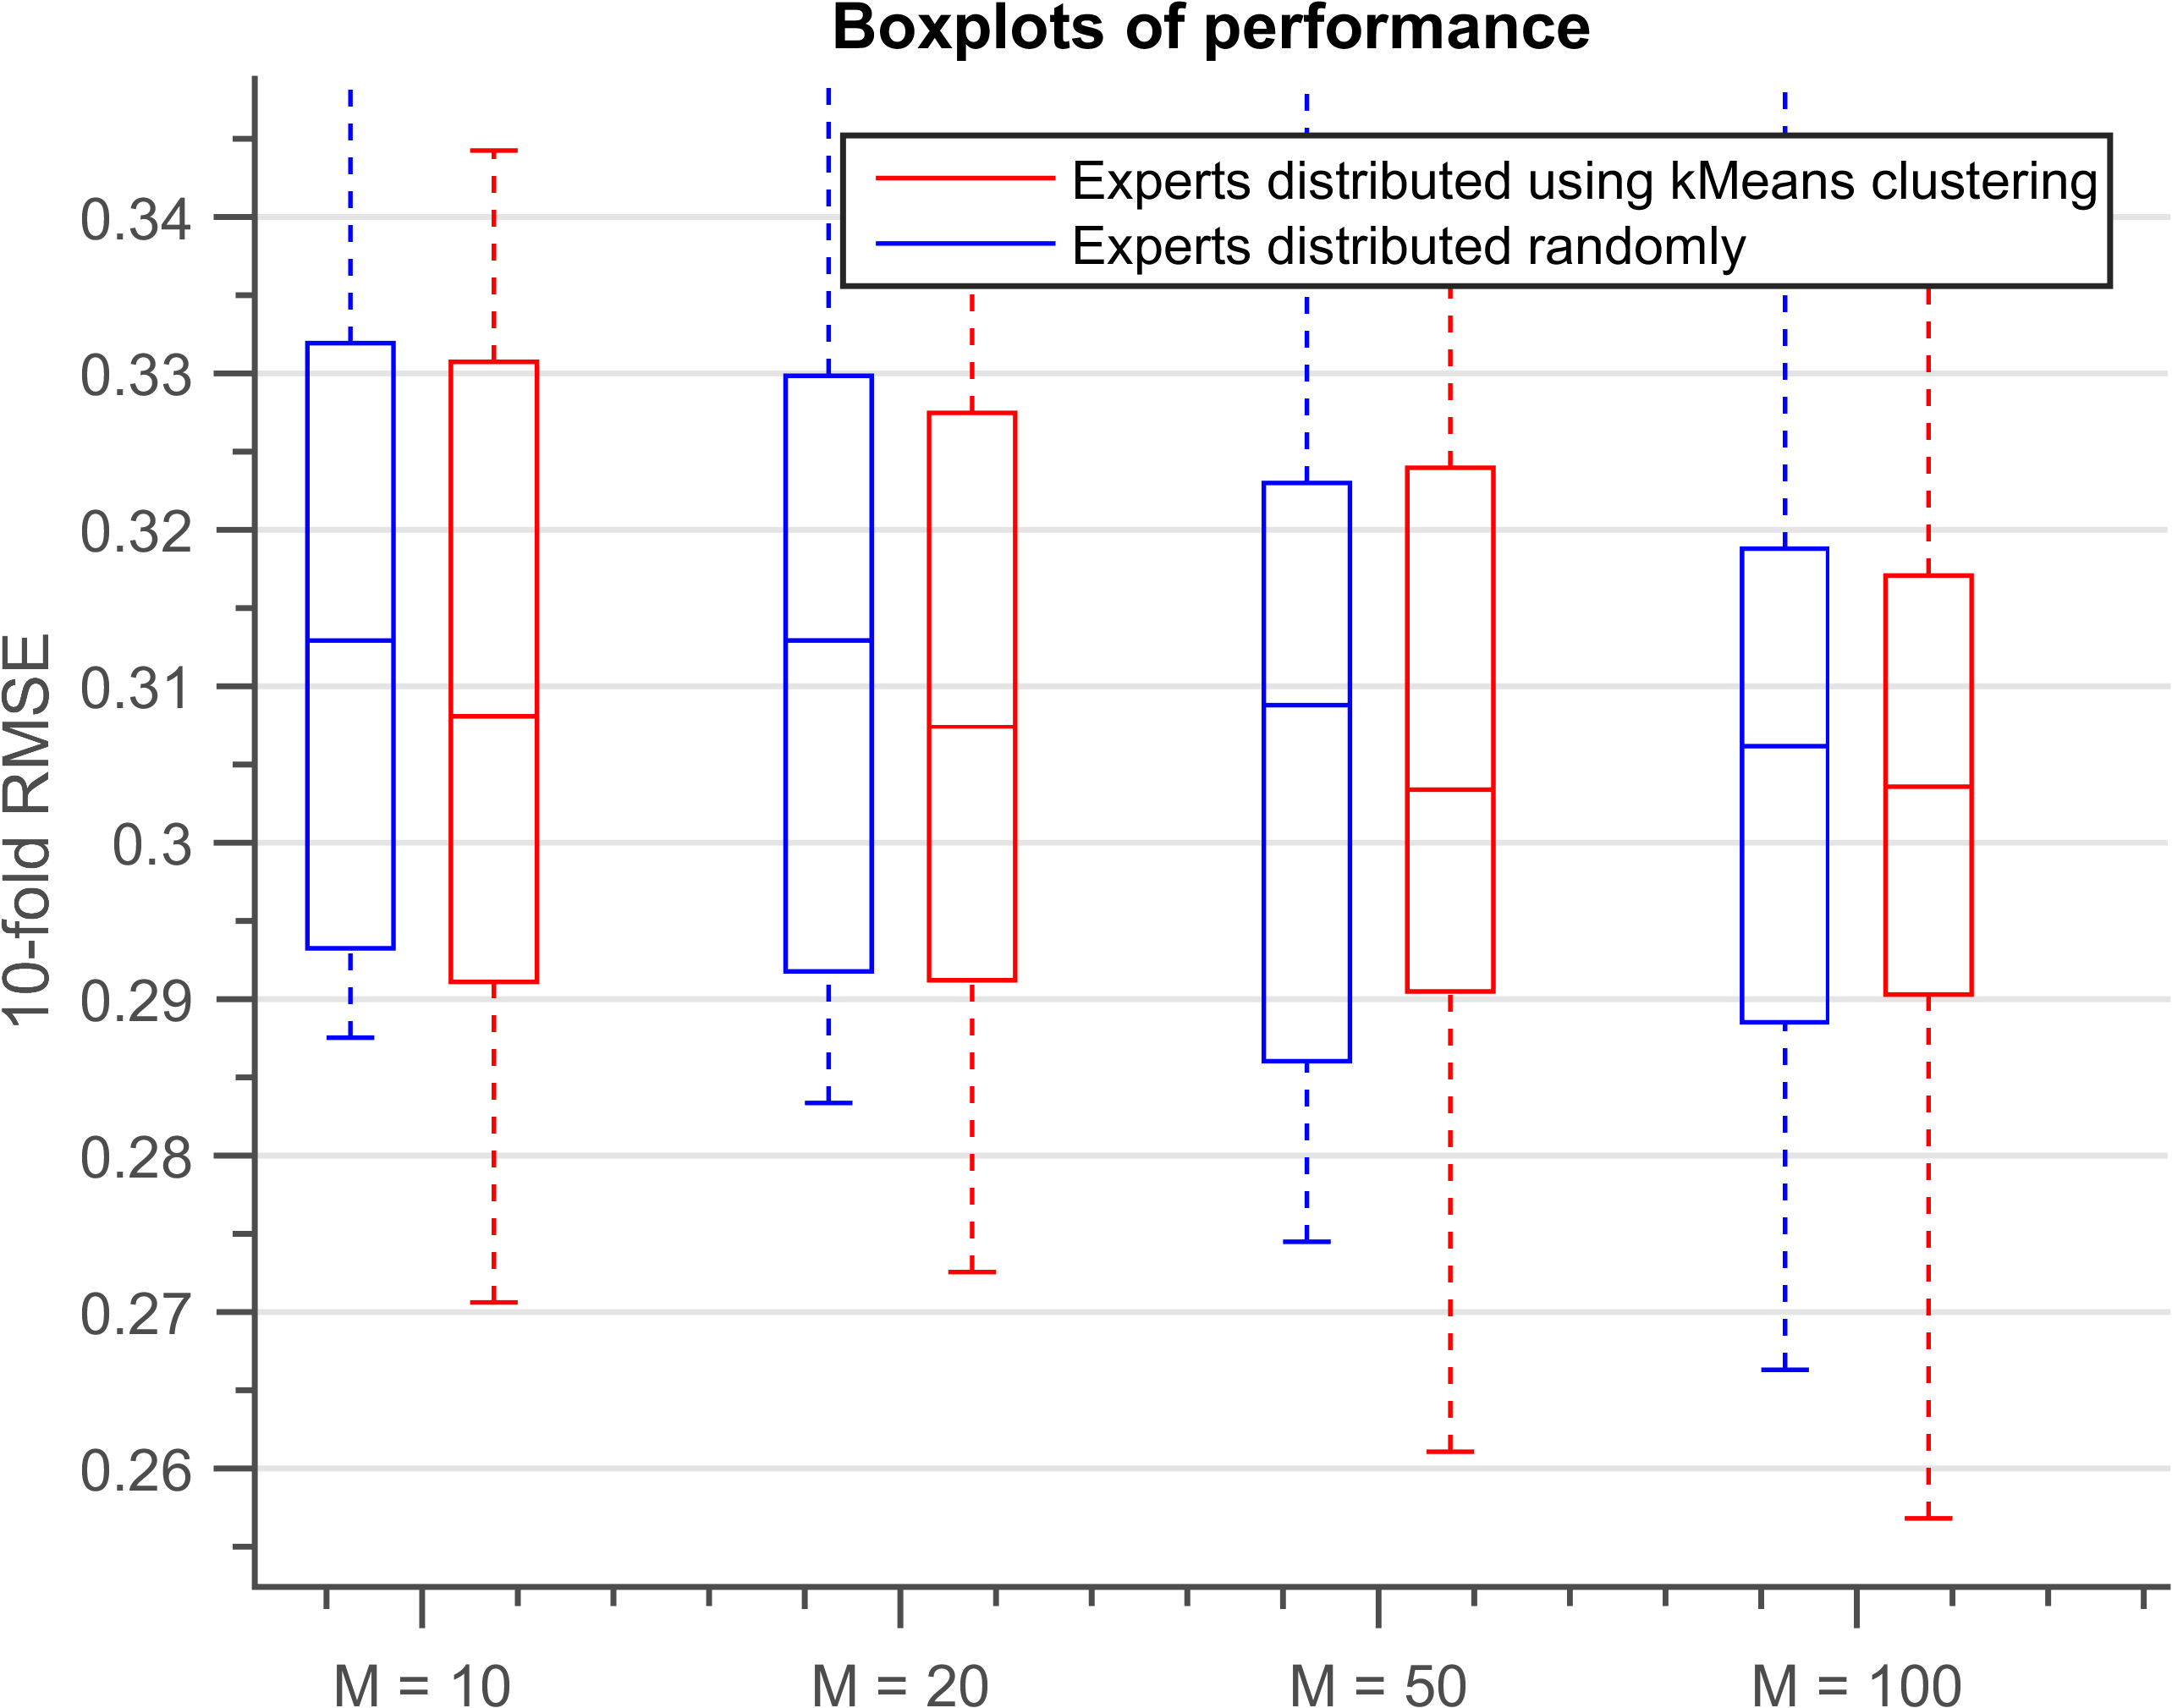
\includegraphics[width=0.45\textwidth]
        {images/boxPlotsOfPerformance_243}
        \label{boxPlotsOfPerformance_243}
  }\quad
  
       \caption{Results of distributed GP Approximation on a toy-data set of size \(N= 1000\)}\label{figGPPredictionDistributed}
\end{figure}

\section{Discussion}
The calculation of posterior distribution in GPs becomes computationally intractable for large data sets. Calculating the precision matrix is an operation of computational complexity \(\mathcal{O}(N^{3})\), putting a limit of \(N \sim 10^4\) data points for model building. This chapter \ref{chapSparseGPRegression} describes the state of art for scaling up GPs for regression tasks. There exist two methods to scale up GPs, the first called sparse methods which uses a set of inducing inputs to reduce the computational cost of calculating the precision matrix. The second called distributed GP which divides the data set into another set of smaller datasets called experts, distributing the model building into several batches. 

Sparse methods use Nystr\"{o}m approximation rewriting the Gram matrix as equation \ref{subSecSamplingFunctionsGPPrior}, thereby reducing the computational complexity to \(\mathcal{O}(NM^{2})\) (M << N), \(M\) being the number of inducing points. Through experiments on a toy-dataset it can be shown that we can set \(M \sim N/10\) for randomly distributed inducing points and \(M \sim N/50\) when we optimize the locations of inducing points. This approximation pushes the limit of GP Regression to \(N \sim 10^6\) data points. Distributed GPs distributes the GP Regression tasks into several batches, thereby reducing the computational complexity to \(\mathcal{O}(NP^{3})\) (P<<N), \(P\) being the number of points in an expert. Through experiments on a toy-dataset we demonstrate that \(P \sim N/100\) does not effects the regression task significantly. In fact we can further reduce \(P\) if we enable repetition of points between experts. This enables to scale GPs to any number of data-points, we will demonstrate this by running a GP regression on millions of data-points in this manuscript (section \ref{}). 

There are several reasons why GPs should be preferred to perform regression tasks. GPs provide a probabilistic framework to define a family of functions, while the covariance functions allows to incorporate a wide range of assumptions (Chapter \ref{chapStructureWithCovariance}). GPs are computationally tractable, given a covariance function and observations, the predictive distribution can be calculated exactly. By providing a closed form expression of marginal likelihood GPs provide a powerful method to automatically select hyperparameters. Although GPs suffer in presence of large data sets, there exist several approximate methods to scale GPs to millions of data points. 






\part{Incorporating structure in Gaussian Process Regression}\label{partIncorporatePattern}
\chapter{Basic Covariance Functions}
\label{chapBasicCovarianceKernels}

After accounting for the zero mean, a GP prior can be completely parametrized by the covariance function. Hence the problem of learning in a Gaussian Process is exactly the problem of finding suitable properties of the covariance function \cite{rasmussen2006gaussian}. The covariance function consists of two parts a functional form (which specifies the shape of functions in the hypothesis space) and a set of hyper-parameters (which define the probability of a function in the hypothesis space). In section \ref{secHyperParameter} we have seen in detail how to automatically choose hyper-parameters, the part \ref{partIncorporatePattern} of this thesis will detail how to choose the functional form. 

\textbf{There exist methods in the literature to automatically choose the functional form of a covariance function \cite{duvenaud-thesis-2014, lloyd2014automatic, automaticStatistician}, we will not detail those methods here.}


This part of the thesis shows how to incorporate prior information of patterns into building GP models. The chapter \ref{chapBasicCovarianceKernels} shows few basic kernel types, while the chapter \ref{chapCombiningBasicCovariances} shows how to combine these basic kernels together and incorporate more complex patterns. This part \ref{partIncorporatePattern} is heavily inspired from works of \cite{duvenaud-thesis-2014, wilson2014thesis, lloyd2014automatic, durrande2001etude}. 

The covariance functions discussed in this chapter are common in the machine learning literature, but unfortunately not often used to build engineering models. The original contribution of chapter \ref{chapBasicCovarianceKernels} is application of basic kernels to build meaningful engineering models. We build a model using spectral mixture kernel (section \ref{subSecSMKernelApplication}) to automatically identify structural dynamics parameters \cite{chiplunkar2017operational}. We also apply a change-point kernel (section \ref{subsubsecCh4ApplicationCP}) to detect start of plasticity in an elastic beam and start of flow separation on an airfoil \cite{chiplunkar:hal-01555401}.  

\textbf{This chapter unfolds as follows}

\section{Properties}\label{secPropertiesOfCovariance}
A kernel is a function that maps any pair of inputs into a scalar \(\mathcal{R}\), the inputs can be scalars themselves, vectors, categorical variables or even images. The covariance of a GP is an example of a kernel, which specifies covariance of a pair of random functions \(f(x_{i})\) and \(f(x_{j})\) situated at points \(x_{i}\) and \(x_{j}\) (mostly written as a function of \(x_{i}\) and \(x_{j}\)). 

Most of the learning algorithms work on distance measures, i.e. if two points are closer then their observations will also tend to be similar. Covariance functions are methods to specify the measure of distance in a GP Regression. If two points have a high value of covariance, then they are similar and hence will have similar value of outputs (\(y\)). Therefore, by defining a covariance function we encode biases into our family of functions. Biases based on smoothness (section \ref{subSecCh4SEKernel}), linearity (section \ref{secCh4RevisitBLR}), differentiability (section \ref{subsecCh4MaternKernel}) etc can be easily encoded using simple covariance functions.

For zero mean GPs as specified in section \ref{subSecCH2MeanFunction} a covariance function between \(f(x_{i})\) and \(f(x_{j})\) can be written as equation \ref{eqCovariance}.

\begin{equation}\label{eqCovariance}
    k(x_{i}, x_{j}) = cov(f(x_{i}), f(x_{j}))
\end{equation}

A covariance function \(k(x_{i}, x_{j})\) is always symmetric, since: 

\begin{equation}\label{eqSymmetricCovariance}
    k(x_{i}, x_{j}) = cov(f(x_{i}), f(x_{j})) = cov(f(x_{j}), f(x_{i})) =  k(x_{j}, x_{i})
\end{equation}

\(k(x_{i}, x_{j})\) corresponds to a covariance function iff it is a symmetric PSD function \cite{loeve1978probability, durrande2001etude}. Consider for a new random vector \(T = \sum \alpha_{i}f(x_{i})\):

\begin{equation}\label{eqDerivePSDCovariance}
    \begin{aligned}
        var(T) & = cov\left ( \sum_{i} \alpha_{i}f(x_{i}), \sum_{j} \alpha_{j}f(x_{j}) \right ) = \sum_{i}\sum_{j}\alpha_{i}\alpha_{j}cov(f(x_{i}), f(x_{j})) \\
& = \sum_{i}\sum_{j}\alpha_{i}\alpha_{j}k(x_{i}, x_{j})
    \end{aligned}
\end{equation}

Since a variance is always non-negative, hence:
\begin{equation}\label{eqPSDCovariance}
\sum_{i}\sum_{j}\alpha_{i}\alpha_{j}k(x_{i}, x_{j}) \geq 0
\end{equation}

The positive definite requirement means that the covariance kernel corresponds to an inner product in some basis space \cite{bishop2006pattern}. It is generally, difficult to prove if a function is PSD, hence creating new covariance functions is a tough task. A Gram matrix constructed using a covariance function is also a PSD matrix, hence if a covariance function is valid can be easily checked if a Gram matrix is PSD matrix. Fortunately, there exist a wide variety of already available covariance functions this chapter will detail a few of these basic kernels. 

\section{Stationary kernels} \label{secStationaryKernels}
Covariance functions which are purely a function of distance \(\tau = (x-x')\) are called as stationary functions, Whereas covariance functions which are functions of absolute value of distance \(\tau = |x-x'|\) are called as isotropic covariance functions. Stationary covariance functions remains unchanged if the points \(x, x'\) are translated. Hence a family of functions defined by stationary kernels will have similar local features throughout the input domain. 

\textit{Bochner's theorem} states that Fourier transform of a stationary covariance function exists and is a positive finite measure. If \(k(\tau)\) is a stationary covariance function then \(S(s)\) is its Fourier transform, also called the power spectrum or spectral density \cite{bochner1959lectures, Stein1999Springer, cox1977theory}. Positive finite measure in this context means that \(S(s)\) is non-negative for all frequencies \(s\) and integral of \(S(s)\) is finite.

\begin{equation}
    k(\tau) = \int S(s) e^{2 \pi is^{T} \tau}ds
\end{equation}

\begin{equation}
    S(s) = \int k(\tau) e^{-2 \pi is^{T} s}d\tau 
\end{equation}

The power spectrum is a more interpretable method of understanding constituent functions in a hypothesis space. The covariance function probabilistically defines a hypothesis space, the power spectrum corresponding to a covariance function tells us the strength/power of the frequencies in this hypothesis space. If a power spectrum has more power at lower frequencies, then the constituent functions in its hypothesis space will be smooth. Whereas, if the power spectrum has more power at higher frequencies, then the constituent functions in its hypothesis space will be faster varying. 

\subsection{Squared Exponential Kernel}\label{subSecCh4SEKernel}
We have already encountered the Standard Exponential (SE) kernel in section \ref{subSecCH2Covariance}. It is one of the most widely used kernel because it defines a hypothesis space of infinitely differentiable (infinitely smooth) functions. The SE kernel is Gaussian in shape (equation \ref{eqnKSESquaredExponential}), which makes its Fourier transform also Gaussian in shape (equation \ref{eqnSSESquaredExponential}).  

\begin{equation}\label{eqnKSESquaredExponential}
k_{SE}(\tau, \theta) = \theta_{amplitude}^2exp[-\frac{\tau^2}{2\theta_{lengthScale}^2}]
\end{equation}

\begin{equation}\label{eqnSSESquaredExponential}
S_{SE}(s, \theta) = \theta_{amplitude}^2  exp[-2\pi \theta_{lengthScale}^2 s^2]
\end{equation}

The two hyper-parameters of the SE kernel are the amplitude hyper parameter (\(\theta_{amplitude}\)) which defines the amplitude of functions and the length-scale hyper-parameter \(\theta_{lengthScale}\), which defines the smoothness of functions. Figure \ref{subFigkernelFunctions} plots the covariance values of SE kernel for varying values of \(\tau\) whereas figure \ref{subFigspectralFunctions} plots the power spectrum for SE kernel for the hyper-parameters (\(\theta_{amplitude}=1\) and \(\theta_{lengthScale}=1\)). If we increase \(\theta_{lengthScale}\) then \(k_{SE}\) will also increase (for same value if \(\tau\) and \(\theta_{amplitude}\)), this means that the far away points will become more similar and hence the constituent functions in the hypothesis space will become more smooth. As length-scale increases the constituent functions tend to become smoother, another way to look at it is using the power spectrum. if we increase \(\theta_{lengthScale}\) then \(S_{SE}\) will start decreasing (for the same value of \(s\) and \(\theta_{amplitude}\)), this means that less power will be allocated to higher frequencies and hence the constituent functions in the hypothesis space will become more smooth (Figure \ref{figGPPriors})

\subsection{Mat\'ern Kernel}\label{subsecCh4MaternKernel}
The Mat\'ern kernel is the second most popular kernel after the squared exponential. This kernel is derived using a Student-t distribution as the power spectrum and calculating its inverse Fourier transform. A student-t distribution has more weight on higher-frequencies (when compared to a Gaussian distribution) and hence gives rise to more non-smooth functions. 

\begin{equation}
k_{Matern}(\nu, \tau, \theta) = \theta_{amplitude}^2\frac{2^{1- \nu }}{\Gamma (\nu)}\left ( \frac{\sqrt{2\nu(\tau))}}{\theta_{lengthScale}} \right )^{\nu}K_{\nu}\left ( \frac{\sqrt{2\nu(\tau))}}{\theta_{lengthScale}} \right)
\end{equation}

Mat\'ern kernel provides the flexibility to define a hypothesis space of functions with varying degree of derivability. The degree of derivability of the functions in the hypothesis space can be set as [\(\nu-1/2\)], i.e.  $\nu = 1/2$ (equation \ref{eqnExponential}) defines family of non-differentiable but continuous functions, $\nu = 3/2$ (equation \ref{eqnMAT32}) defines a family of functions differentiable once and $\nu = 5/2$ (equation \ref{eqnMAT52}) defines a family of functions twice differentiable functions.

\begin{equation}\label{eqnExponential}
k_{Matern}(\nu = 1/2, \tau, \theta) = \theta_{amplitude}^2exp[-\frac{\tau}{\theta_{lengthScale}}]
\end{equation}
\begin{equation}\label{eqnMAT32}
k_{Matern}(\nu = 3/2, \tau, \theta) = \theta_{amplitude}^2 (1 + \frac{\sqrt{3}\tau}{\theta_{lengthScale}}) exp[-\frac{\sqrt{3}\tau}{\theta_{lengthScale}}]
\end{equation}
\begin{equation}\label{eqnMAT52}
k_{Matern}(\nu = 5/2, \tau, \theta) = \theta_{amplitude}^2(1 + \frac{\sqrt{5}\tau}{\theta_{lengthScale}} + \frac{5\tau^2}{3\theta_{lengthScale}^2})
exp[-\frac{\sqrt{5}\tau}{\theta_{lengthScale}}]
\end{equation}

When \(\nu = 1/2\) the Mat\'ern kernel is also called the Ornstein-Uhlenbeck or Exponential kernel, this creates a hypothesis space of non-differentiable continuous functions and was used to explain the Brownian motion \cite{uhlenbeck1930theory}. Figure \ref{subFigkernelFunctions} plots the covariance values of Exponential and Mat\'ern (\(\nu=3/2\)) kernel whereas figure \ref{subFigspectralFunctions} plots the power spectrum for same kernels. We can see that the SE kernel has lowest power for higher frequencies followed by Mat\'ern (\(\nu=3/2\)) and Exponential kernel, meaning that the SE kernel has more smooth functions in its hypothesis space followed by Mat\'ern (\(\nu=3/2\)) and Exponential kernel. 

\begin{figure}[!ht]
  \centering
    \subfigure[{Kernel density for exponential, Mat\'ern (\(\nu=3/2\))and Standard exponential kernel. The hyper-parameters are amplitude (\(\theta_{amplitude} = 1\)) and length-scale (\(\theta_{lengthScale} = 1\))}]
  {
        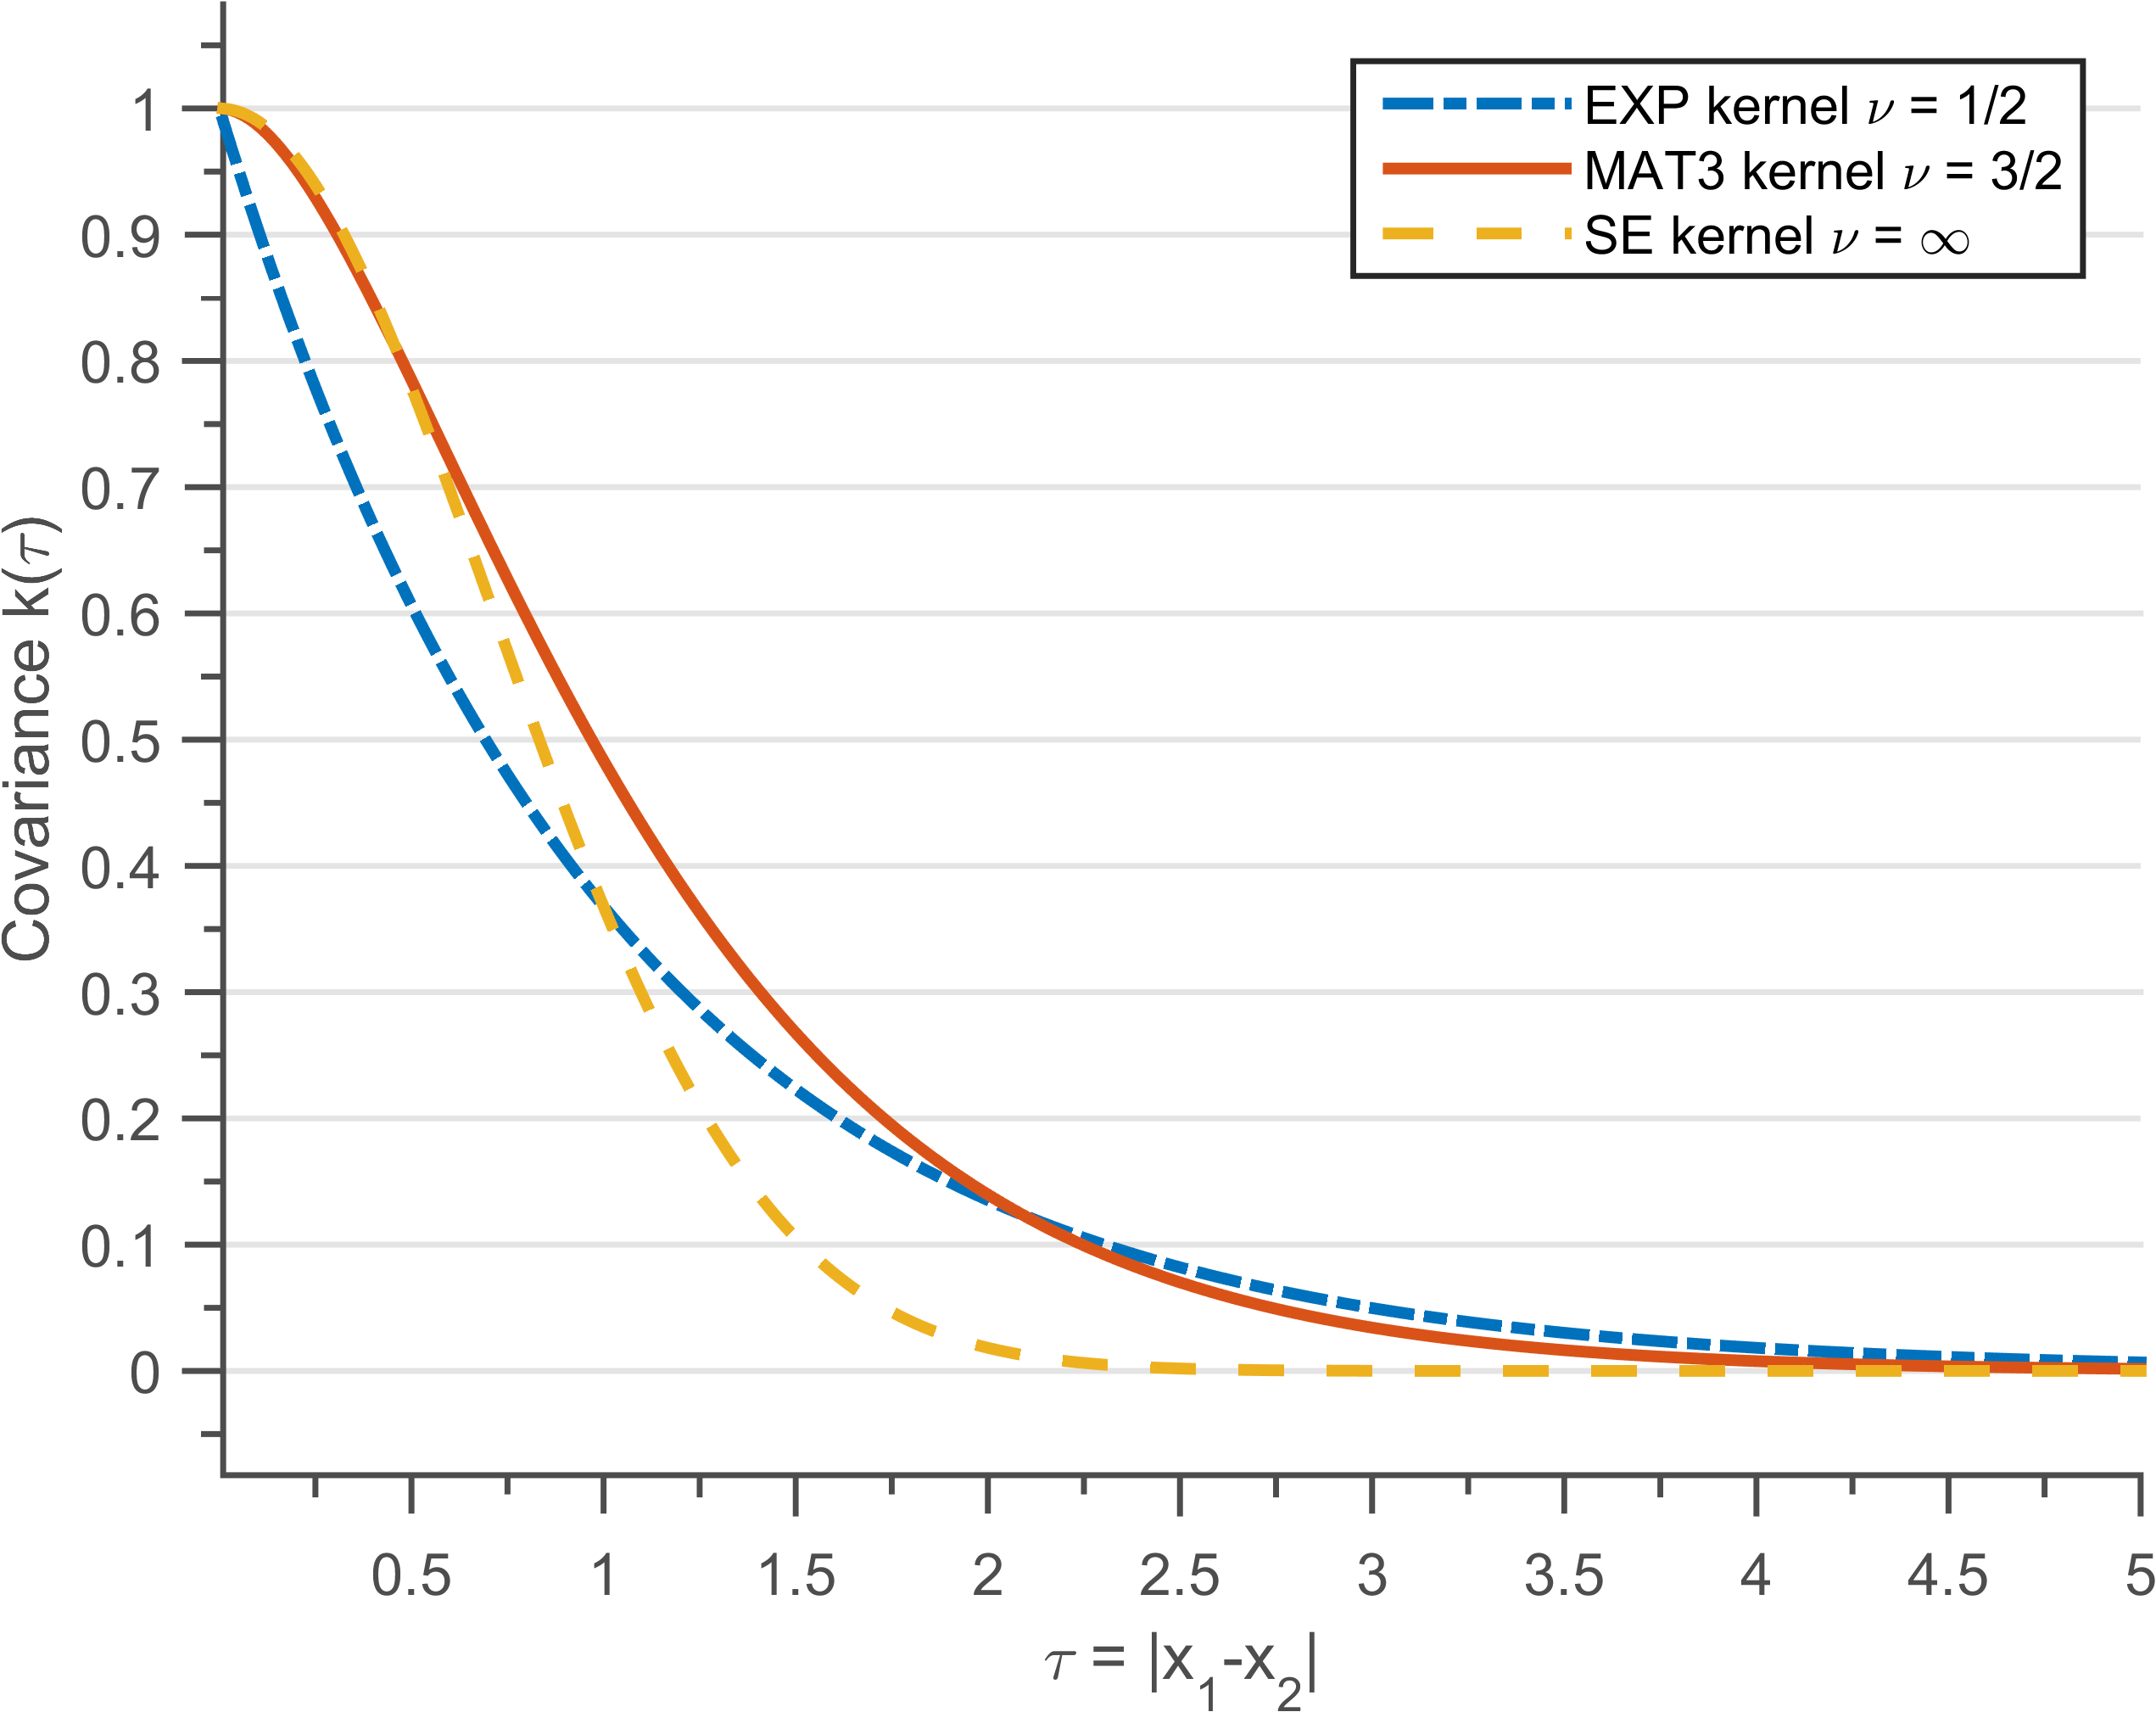
\includegraphics[width=0.45\textwidth]
        {imagesPart2/kernelFunctions}
        \label{subFigkernelFunctions}
  }\quad
\subfigure[{Power spectrum for Exponential, Mat\'ern (\(\nu=3/2\))and Standard exponential kernel. The hyper-parameters are amplitude (\(\theta_{amplitude} = 1\)) and length-scale (\(\theta_{lengthScale} = 1\)). Exponential and Mat\'ern have more power at higher frequencies when compared to SE kernel.}]
  {
        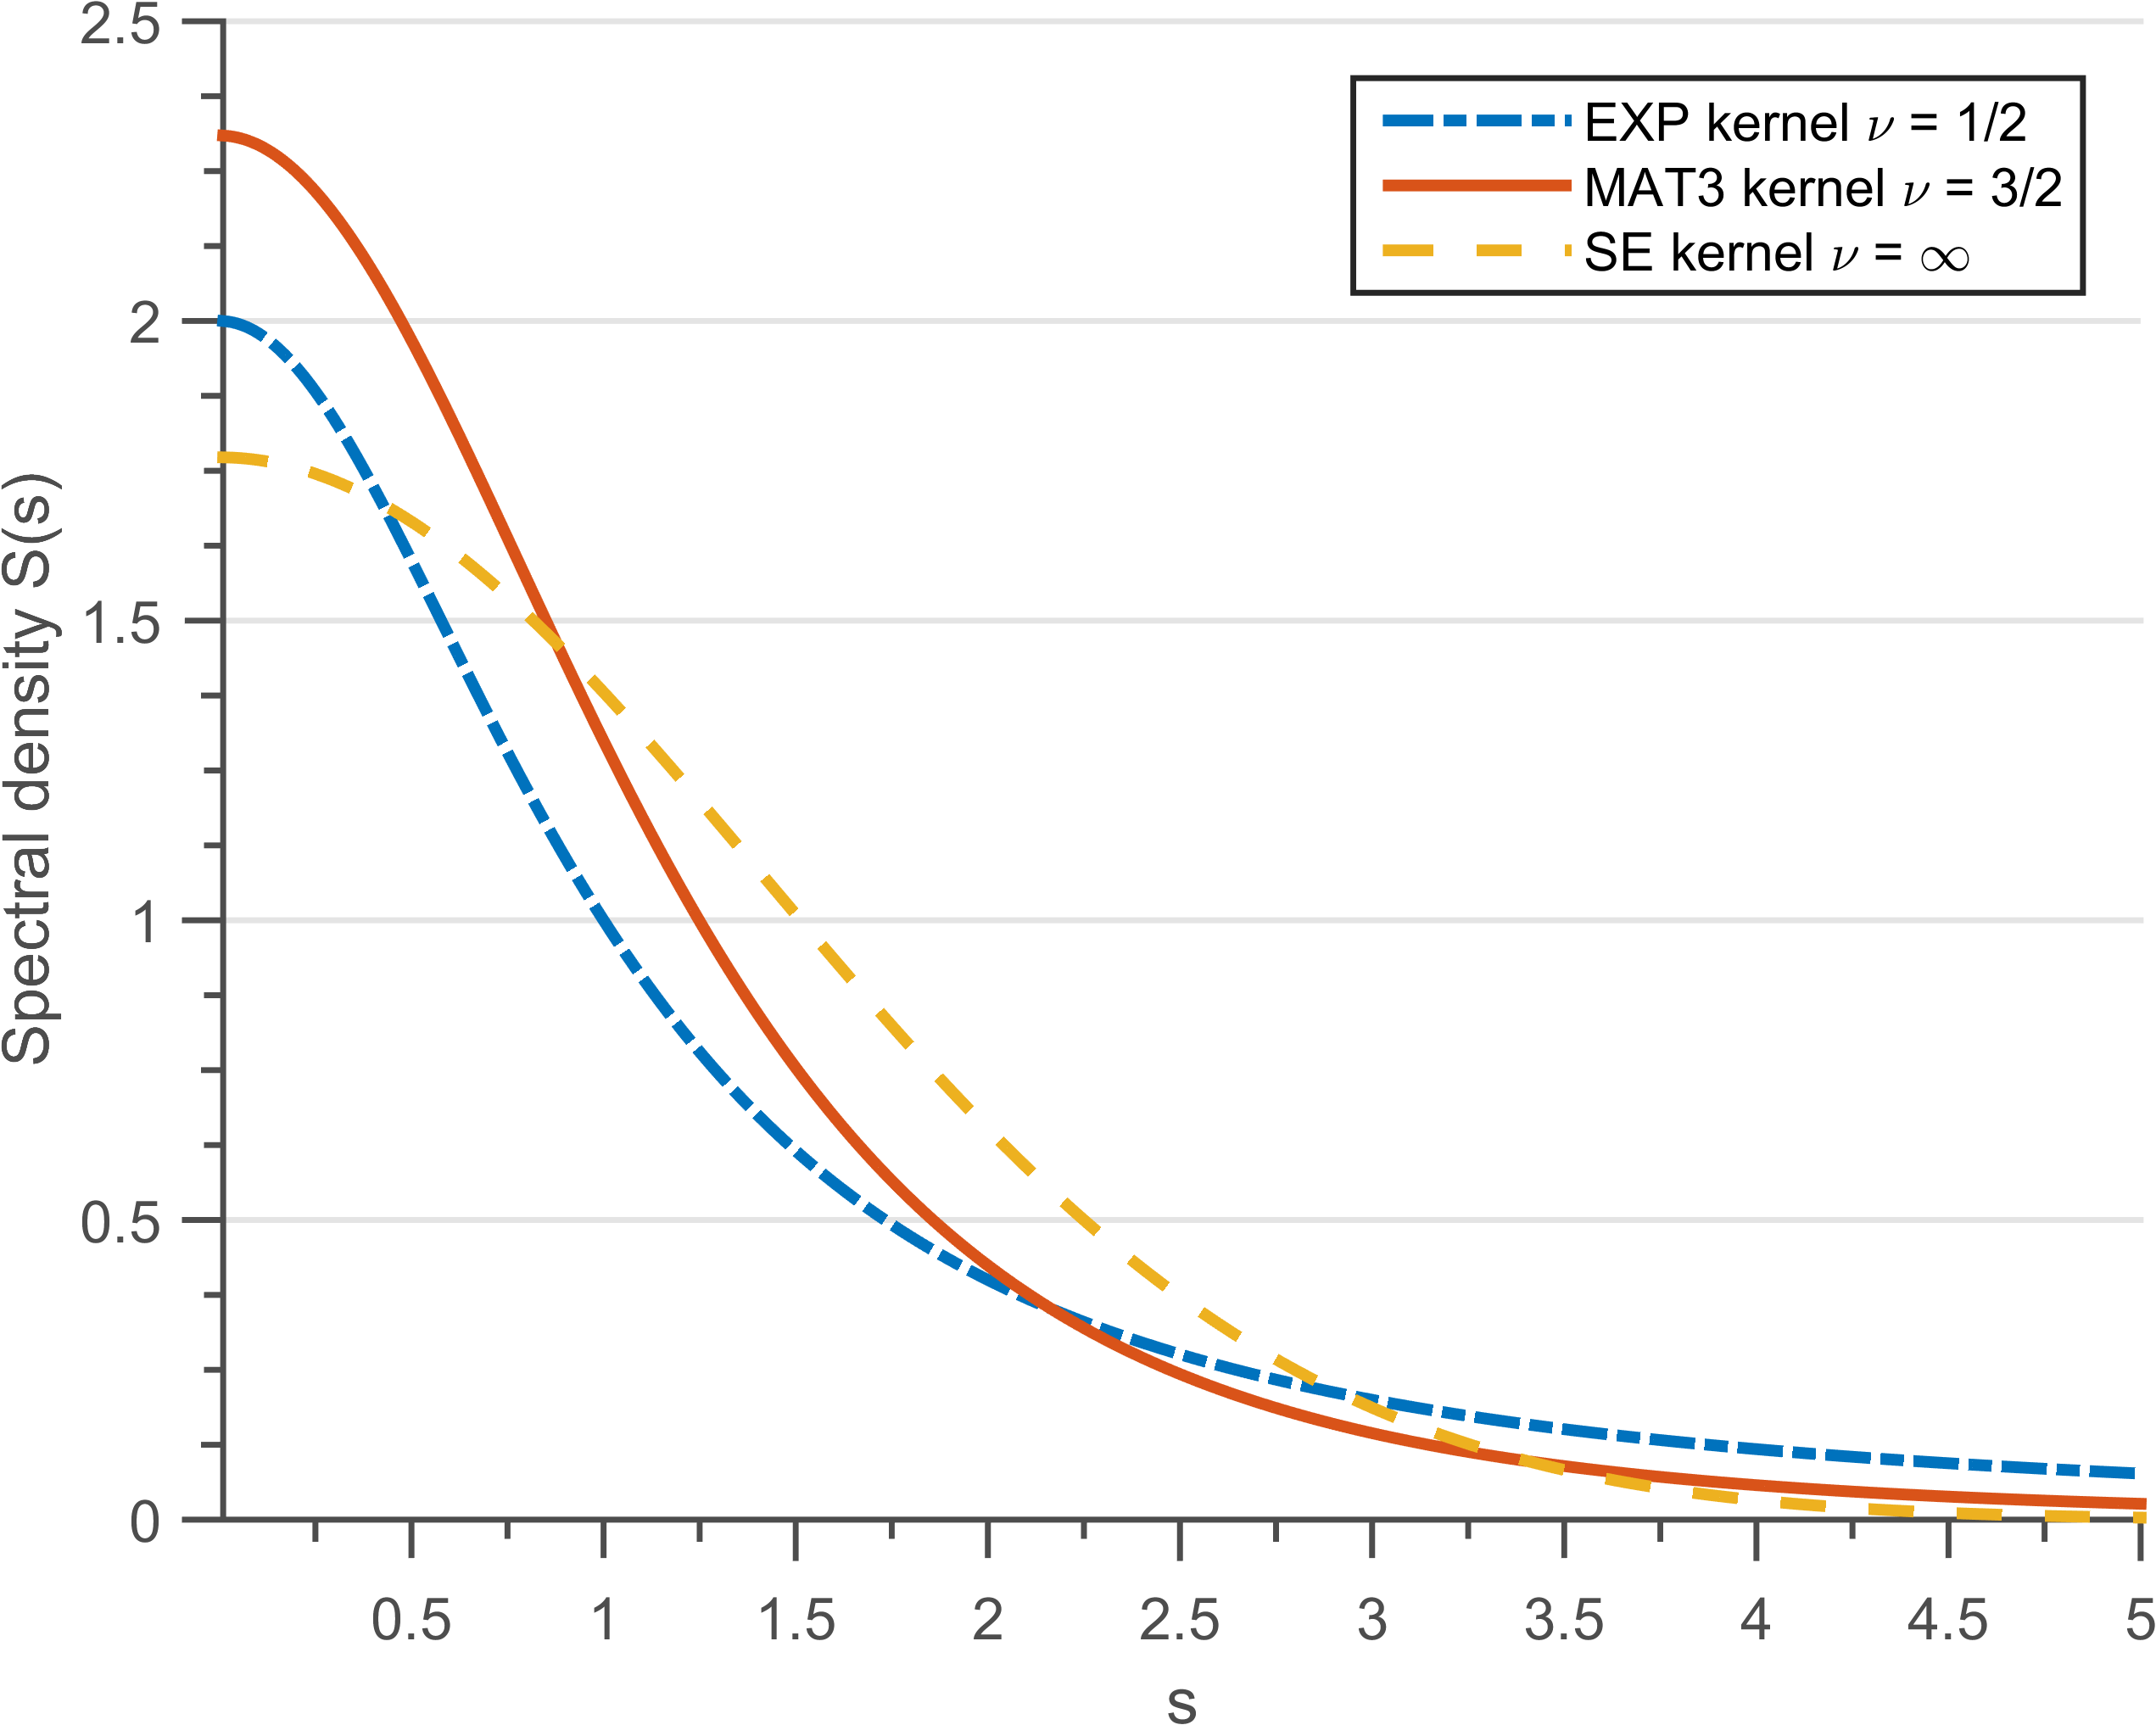
\includegraphics[width=0.45\textwidth]
        {imagesPart2/spectralFunctions}
        \label{subFigspectralFunctions}
  }\quad
\caption{Covariance functions and Power spectrums for three different kernels}
       \label{figKernelAndPowerSpectrums}
\end{figure}

The infinitely smooth assumption of the squared exponential function is unrealistic in several cases \cite{stein2012interpolation}, making the Mat\'ern kernels second most popular choice of kernels. Mat\'ern kernels have been found to have superior performance on datasets with high-dimensions \cite{le2013fastfood}. It is argued that the Mat\'ern kernel accounts for the concentration of measure effect in higher-dimensions. Imagine a high-dimensional orange (it is tough to imagine more than 3 dimensions), but if there was a high dimensional orange than most of its mass will be concentrated in its skin and not its pulp \cite{domingos2012few}. 

\subsection{Experiments}
Let us revisit the dataset \(\mathcal{D}_{2}\) used to calculate the posterior in section \ref{secPosterior} but this time using three different covariance functions. We will use Exponential kernel, Mat\'ern and Standard exponential kernel to compare their performance during GP regression. 

We follow the standard framework of GP regression, we first draw random functions from a the covariance functions to judge the hypothesis space. We next calculate the posterior distribution conditioned on dataset \(\mathcal{D}_{2}\). We finally, optimize the marginal likelihood and compare the final predictions for the three covariance functions. 

Figure \ref{figCh4Priors} shows 5 random functions drawn for a zero mean GP with the three covariance functions for same values of hyper-parameters \(\theta_{lengthscale} = 1, \theta_{amplitude} = 1\), their corresponding covariance functions and power spectrums are whown in figure \ref{figKernelAndPowerSpectrums}. The solid black line defines the mean function, shaded blue region defines 95\% confidence interval (2\(\sigma\)) distance away from the mean. The dashed lines are five functions drawn at random from a GP prior. We can observe that figure \ref{subFigpriorDrawsEXP} draws non-differentiable functions while \ref{subFigpriorDrawsMAT3} and \ref{subFigpriorDrawsSE} draw smoother functions. For the same value of the length-scale, Mat\'ern (\(\nu=3/2\)) kernel has higher variation.

\begin{figure}[!ht]
  \centering
    \subfigure[{Draws from a GP prior with mean zero, Exponential kernel (Mat\'ern with \(\nu = 1/2\)) and hyper-parameters \(\theta_{lengthscale} = 1, \theta_{amplitude} = 1\). Functions drawn from this kernel are non-differentiable.}]
  {
        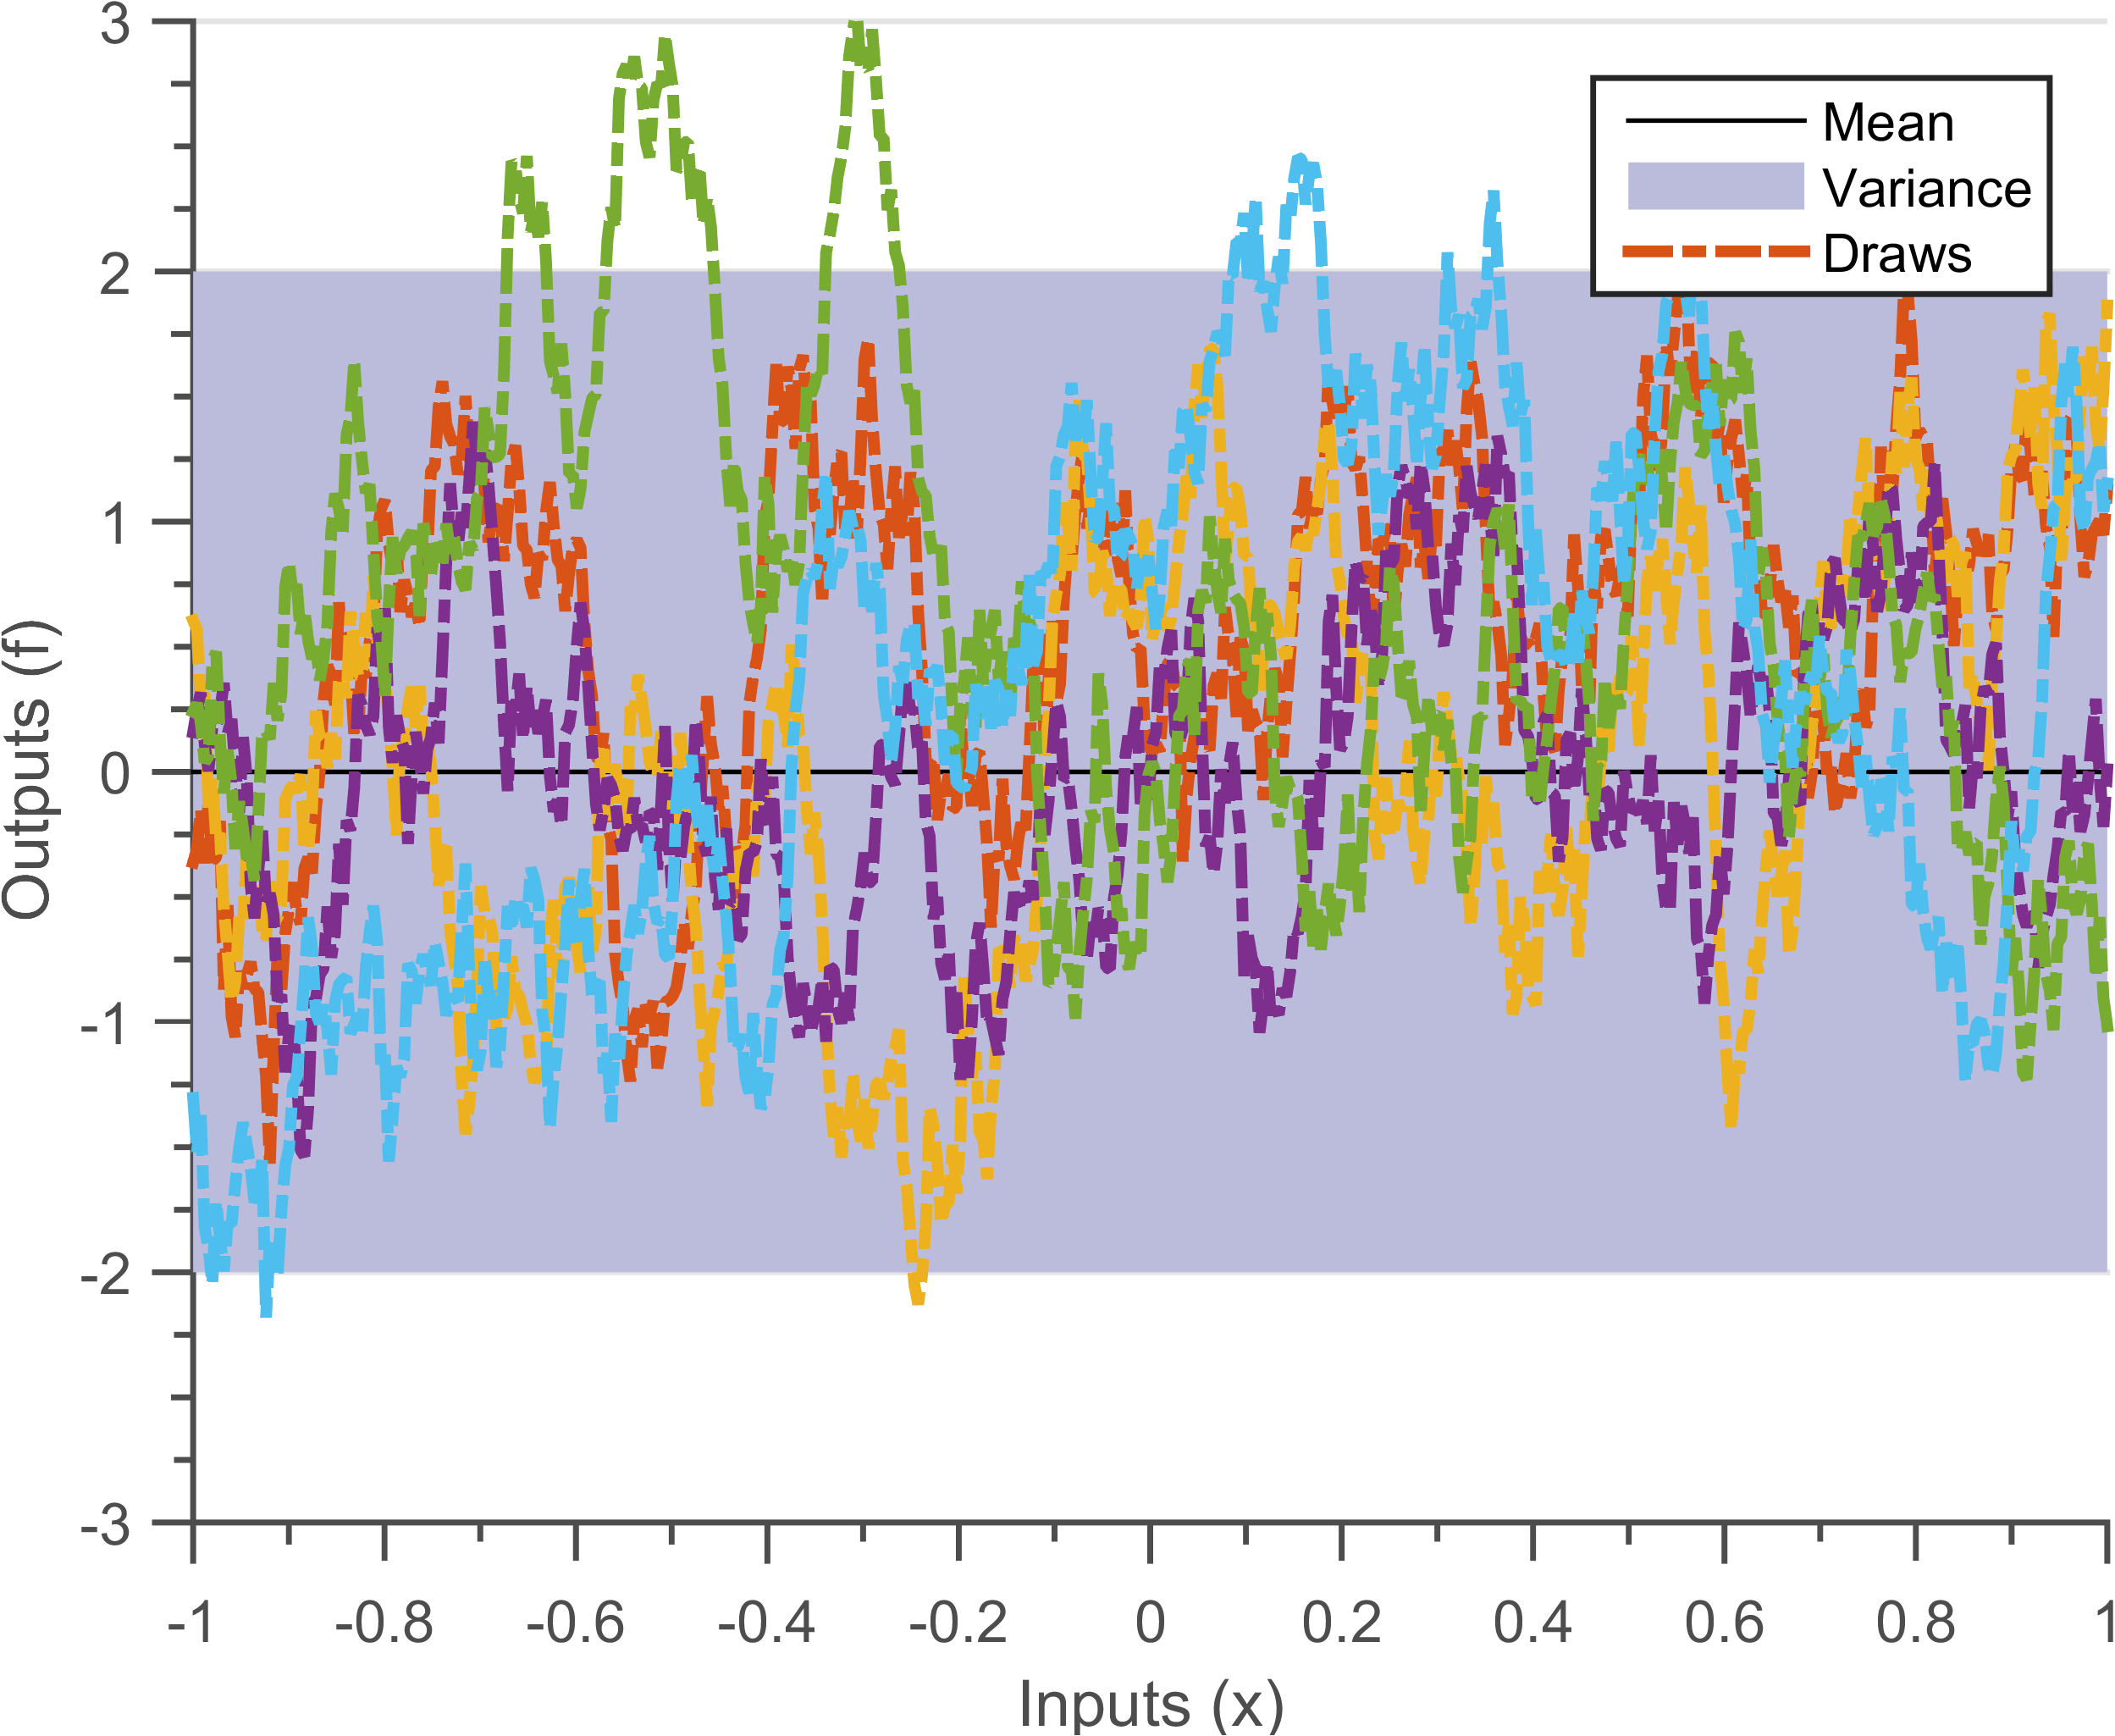
\includegraphics[width=0.29\textwidth]
        {imagesPart2/priorDrawsEXP}
        \label{subFigpriorDrawsEXP}
  }\quad
\subfigure[{Draws from a GP prior with mean zero, Mat\'ern kernel \(\nu = 3/2\) and hyper-parameters \(\theta_{lengthscale} = 1, \theta_{amplitude} = 1\). Functions drawn from this kernel are differentiable only once}]
  {
        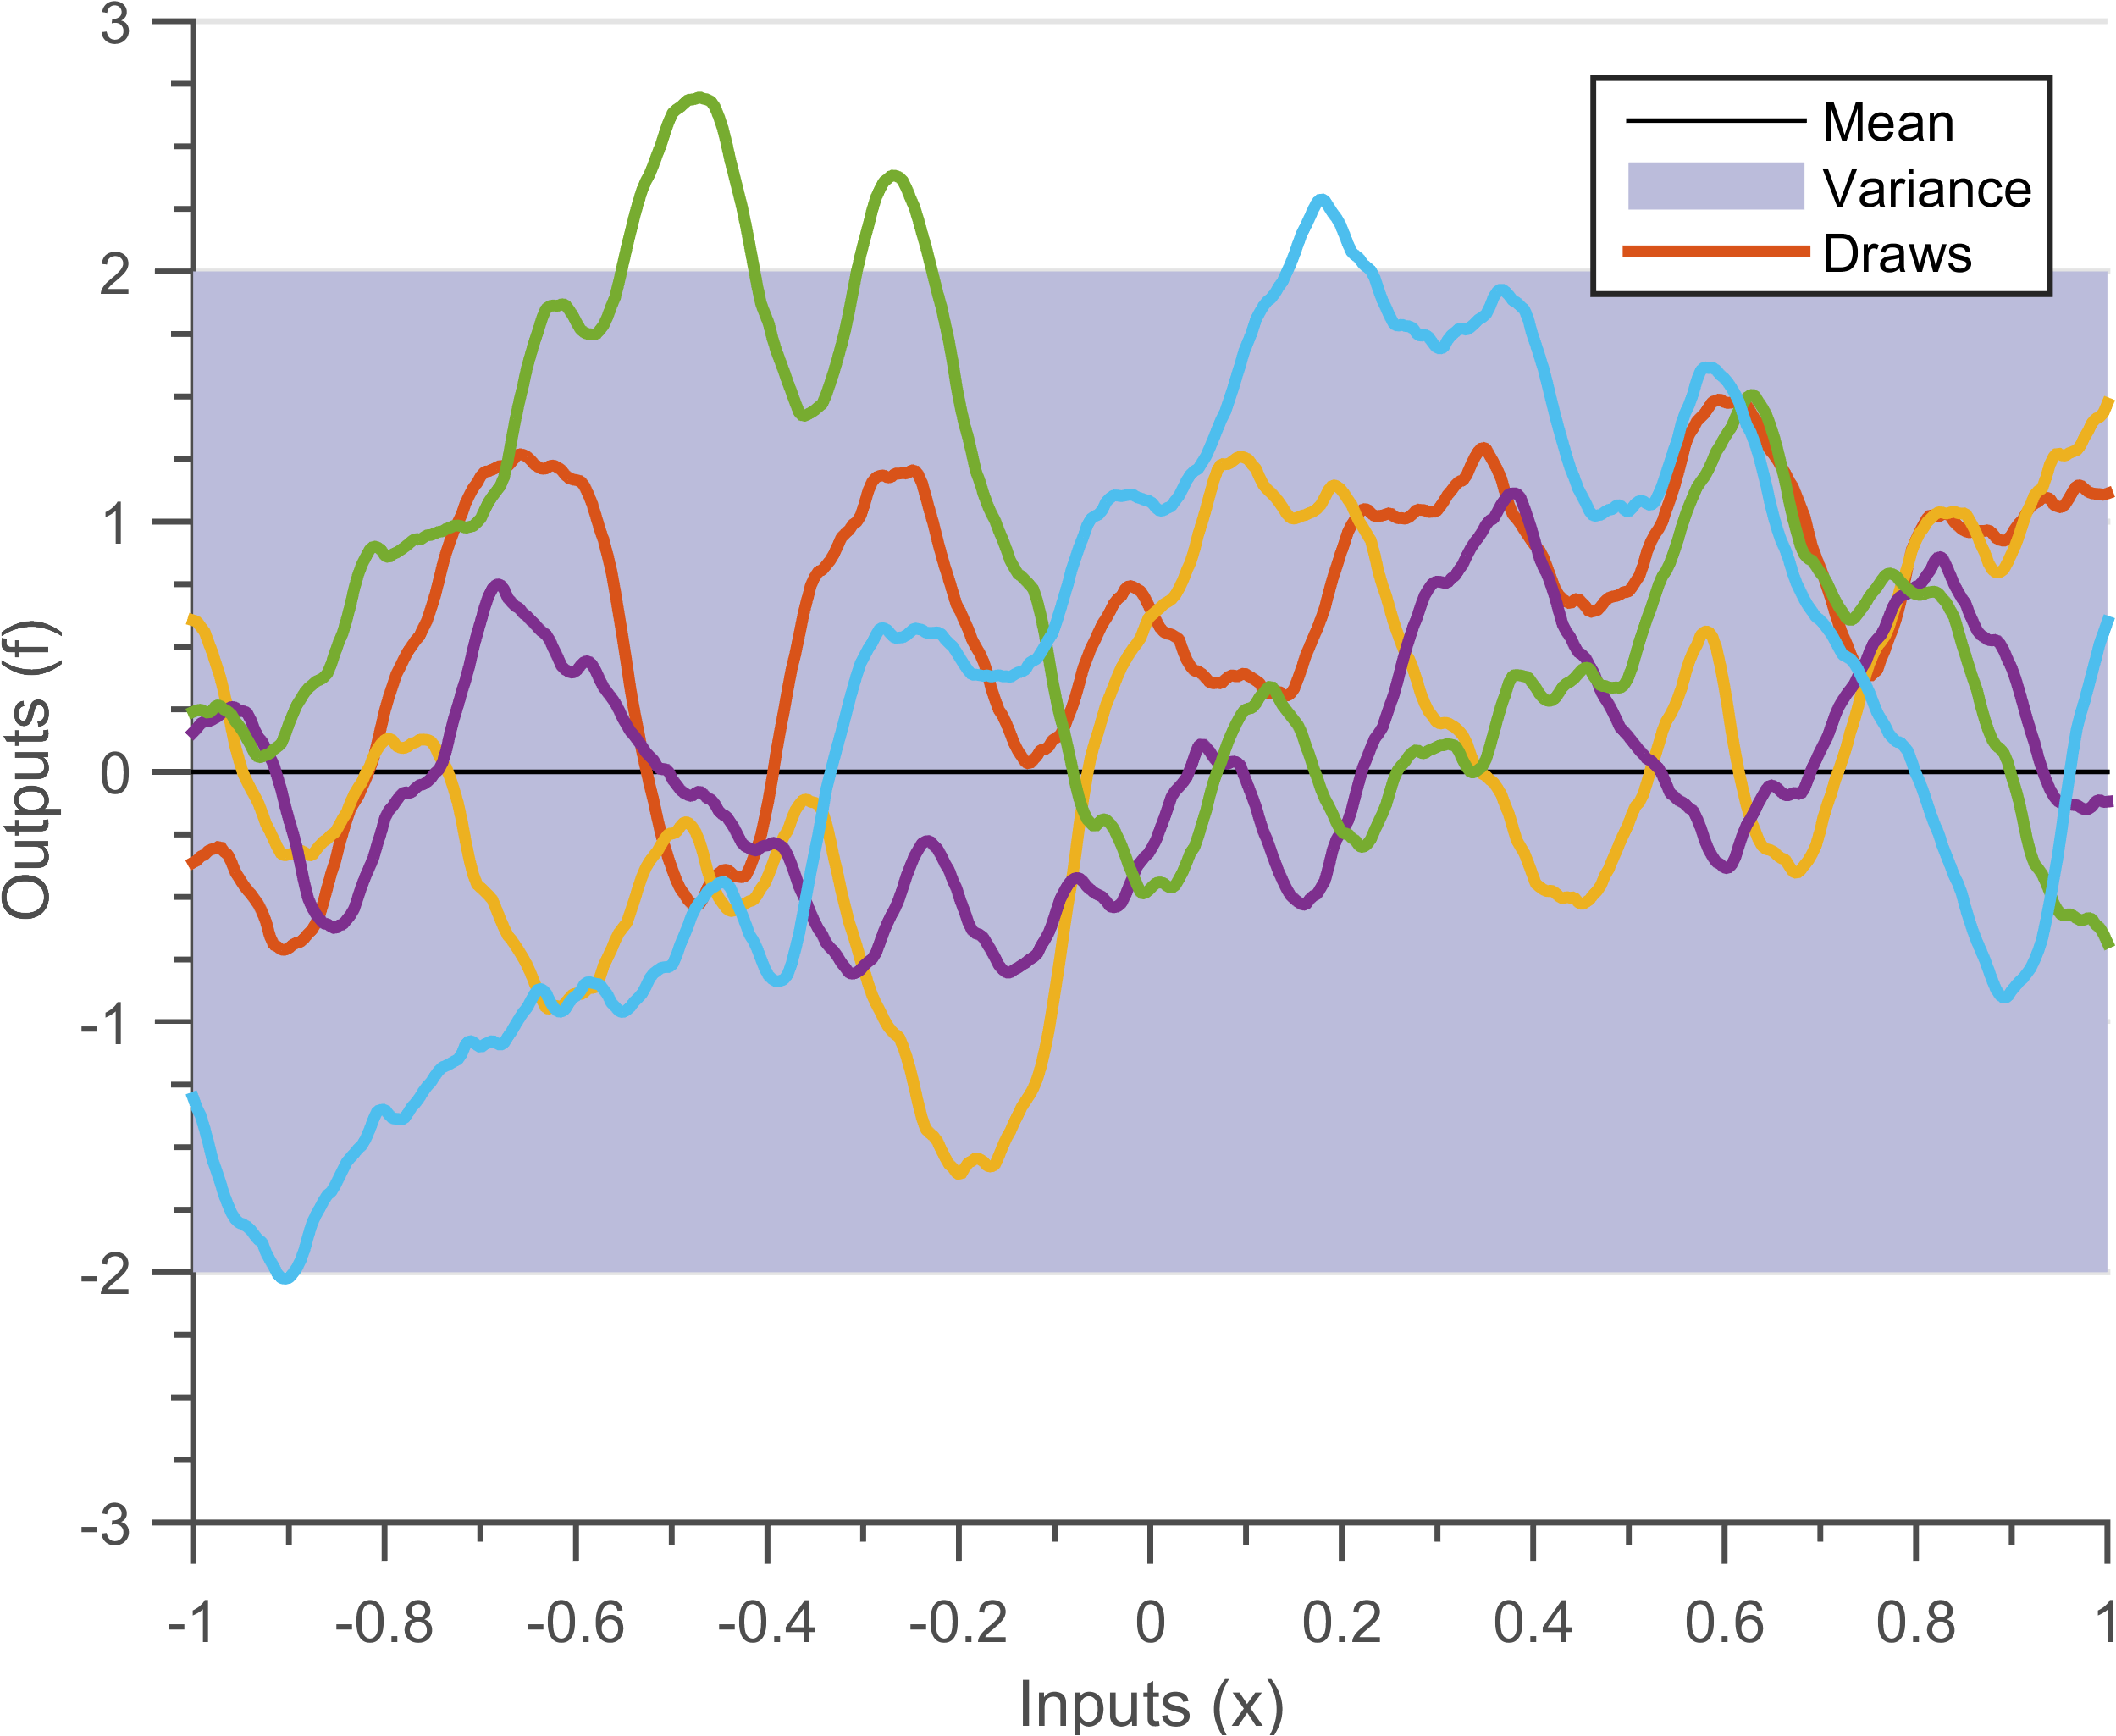
\includegraphics[width=0.29\textwidth]
        {imagesPart2/priorDrawsMAT3}
        \label{subFigpriorDrawsMAT3}
  }\quad
  \subfigure[{Draws from a GP prior with mean zero, Standard Exponential kernel (Mat\'ern with \(\nu = \infty\)) and hyper-parameters \(\theta_{lengthscale} = 1, \theta_{amplitude} = 1\). Functions drawn from this kernel are infinitely differentiable}]
  {
        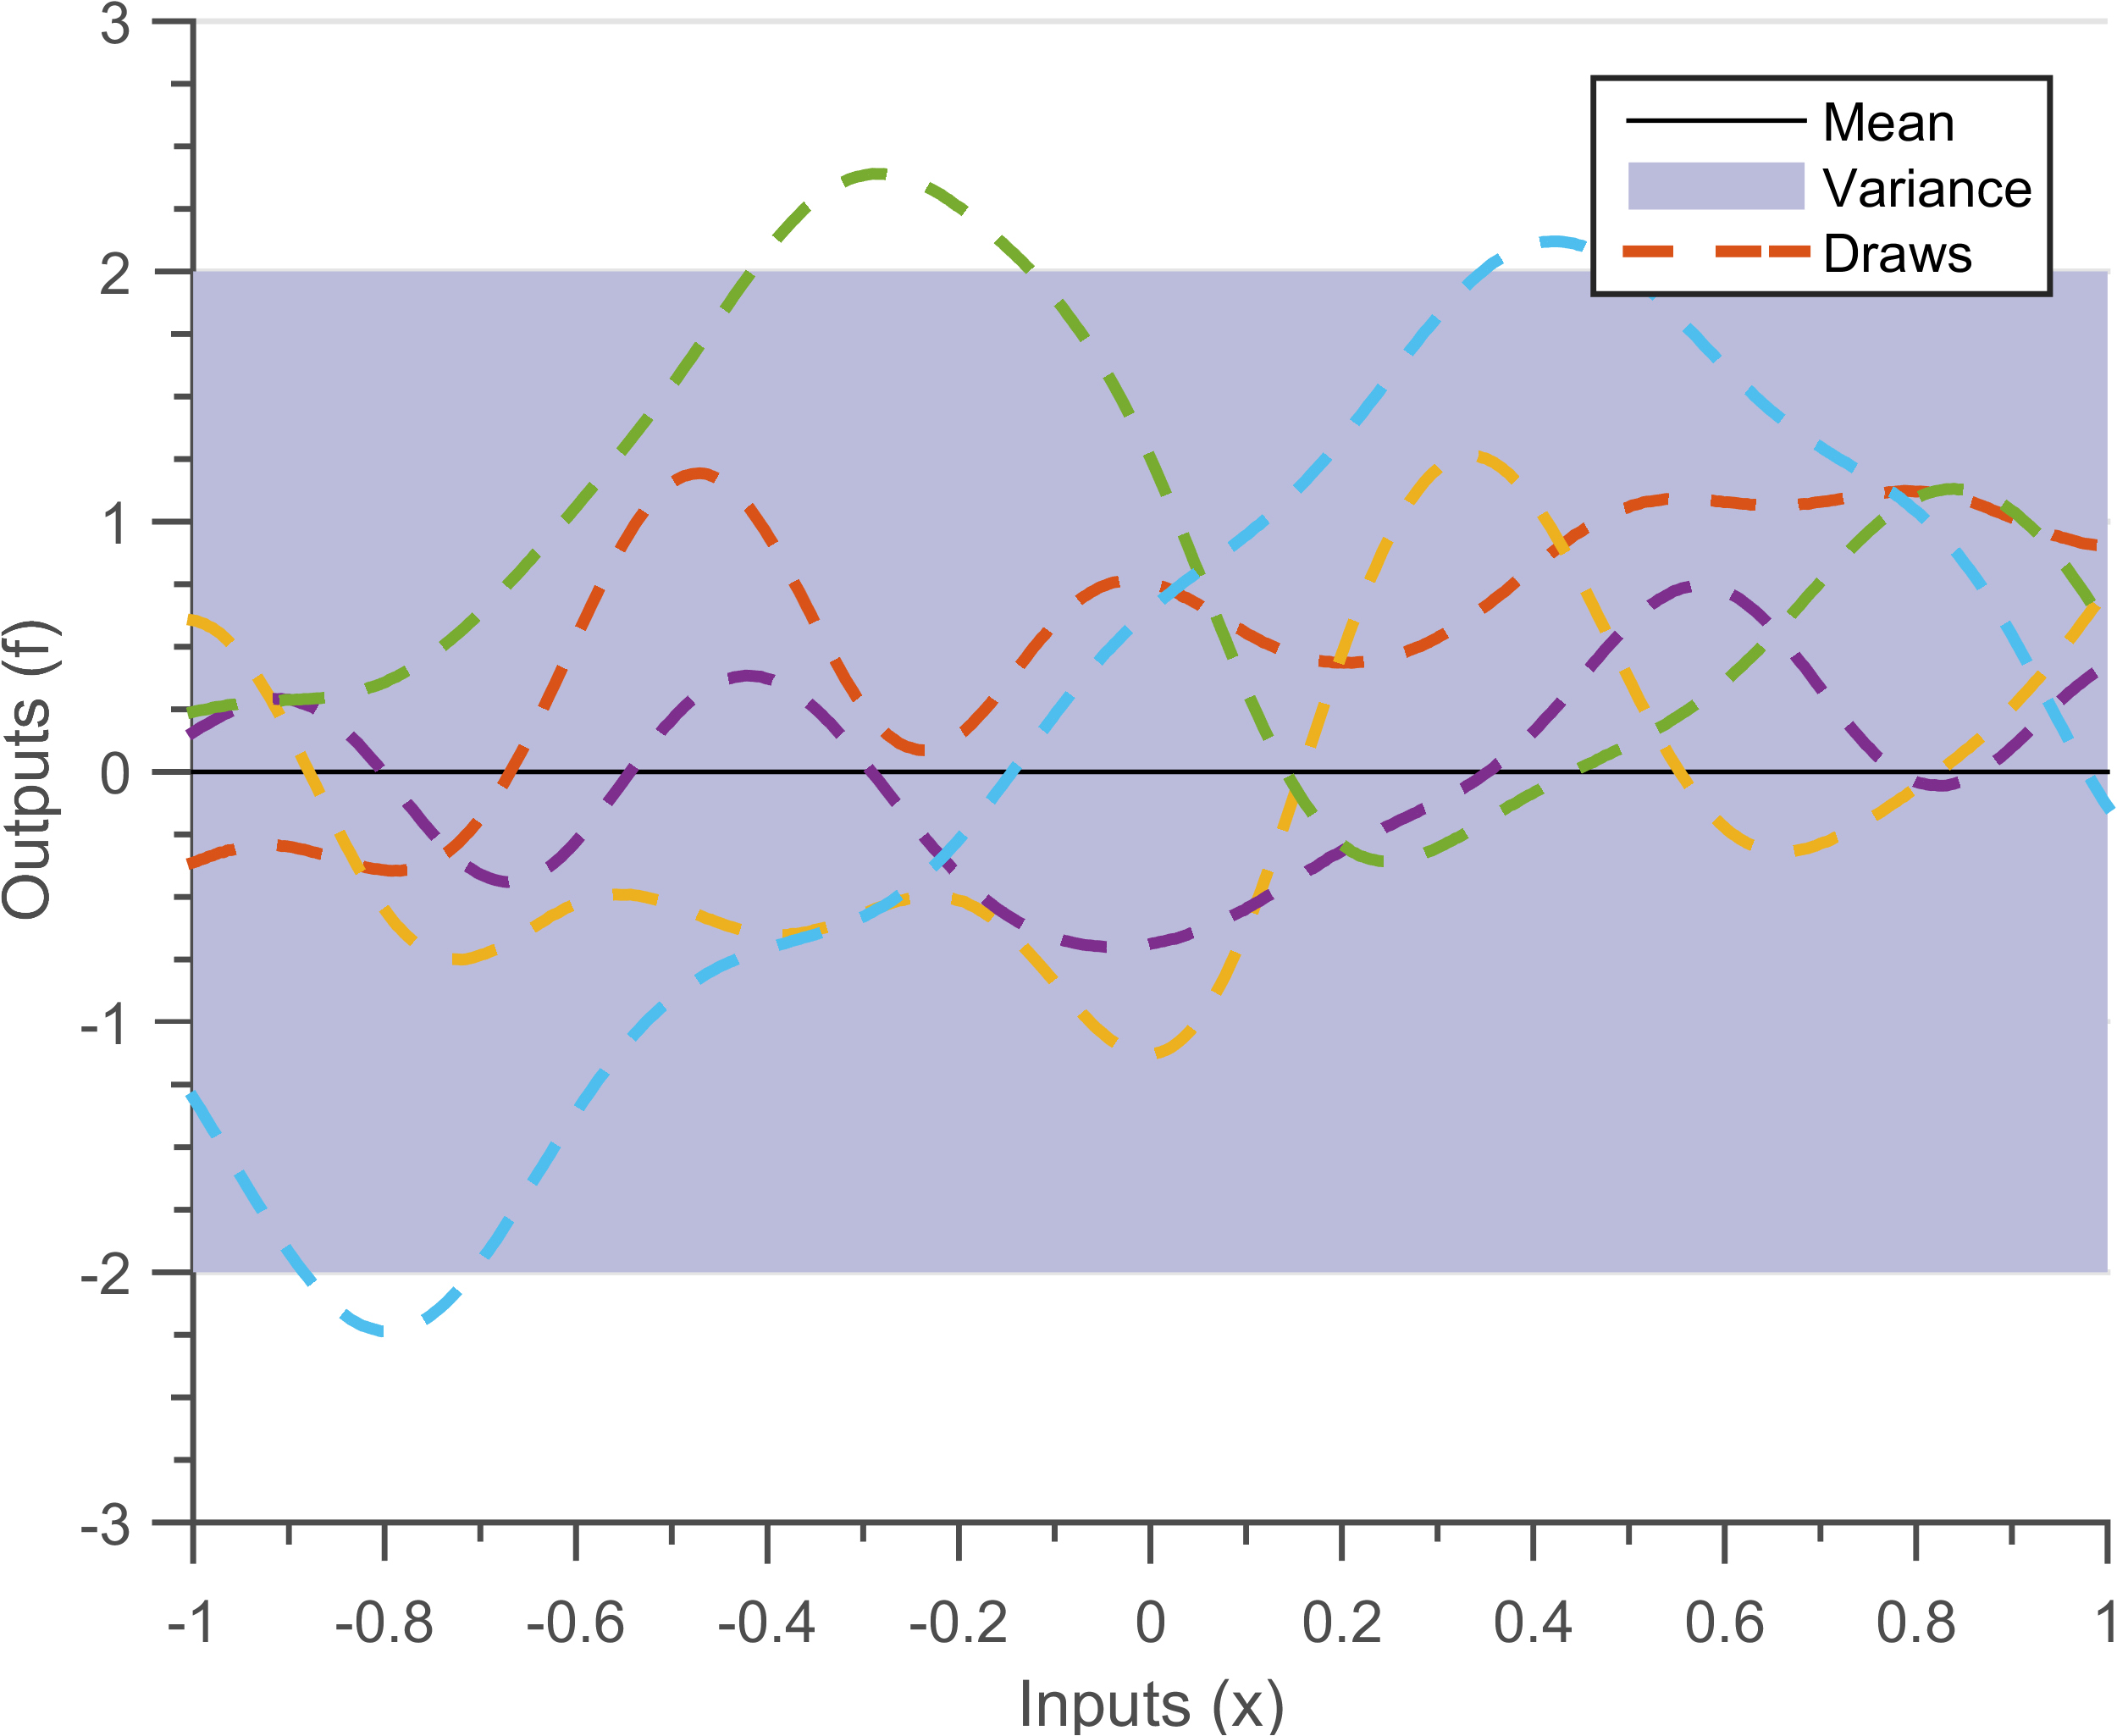
\includegraphics[width=0.29\textwidth]
        {imagesPart2/priorDrawsSE}
        \label{subFigpriorDrawsSE}
  }\quad
\caption{Prior distribution and five random draws from 3 different covariance functions. The solid black line defines the mean function, shaded blue region defines 95\% confidence interval (2\(\sigma\)) distance away from the mean. The dashed lines are five functions drawn at random from a GP prior.}
       \label{figCh4Priors}
\end{figure}

Figure \ref{figpreOptimizedPosteriorCh5} shows the posterior GP conditioned on the dataset \(\mathcal{D}_{2}\) for three different covariance functions with same hyper-parameters. The hyper-parameters are not optimized with respect to the marginal likelihood. For a similar value of hyper-parameters and dataset, Exponential kernel has highest variance followed by Mat\'ern and SE kernel\footnote{Remember the Bias vs Variance trade-off: SE kernel has the most restrictive hypothesis space followed by Mat\'ern \(\nu=3/2\) and Exponential kernel, since infinite differentiability is a stricter assumption}. 

\begin{figure}[!ht]
  \centering
    \subfigure[{Draws from a GP posterior with mean zero and Exopnential kernel (figure \ref{subFigpriorDrawsEXP}) conditioned on the data \(\mathcal{D}_{2}\). The posterior mean passes through the data points, random functions drawn from exponential kernel are non-differentiable}]
  {
        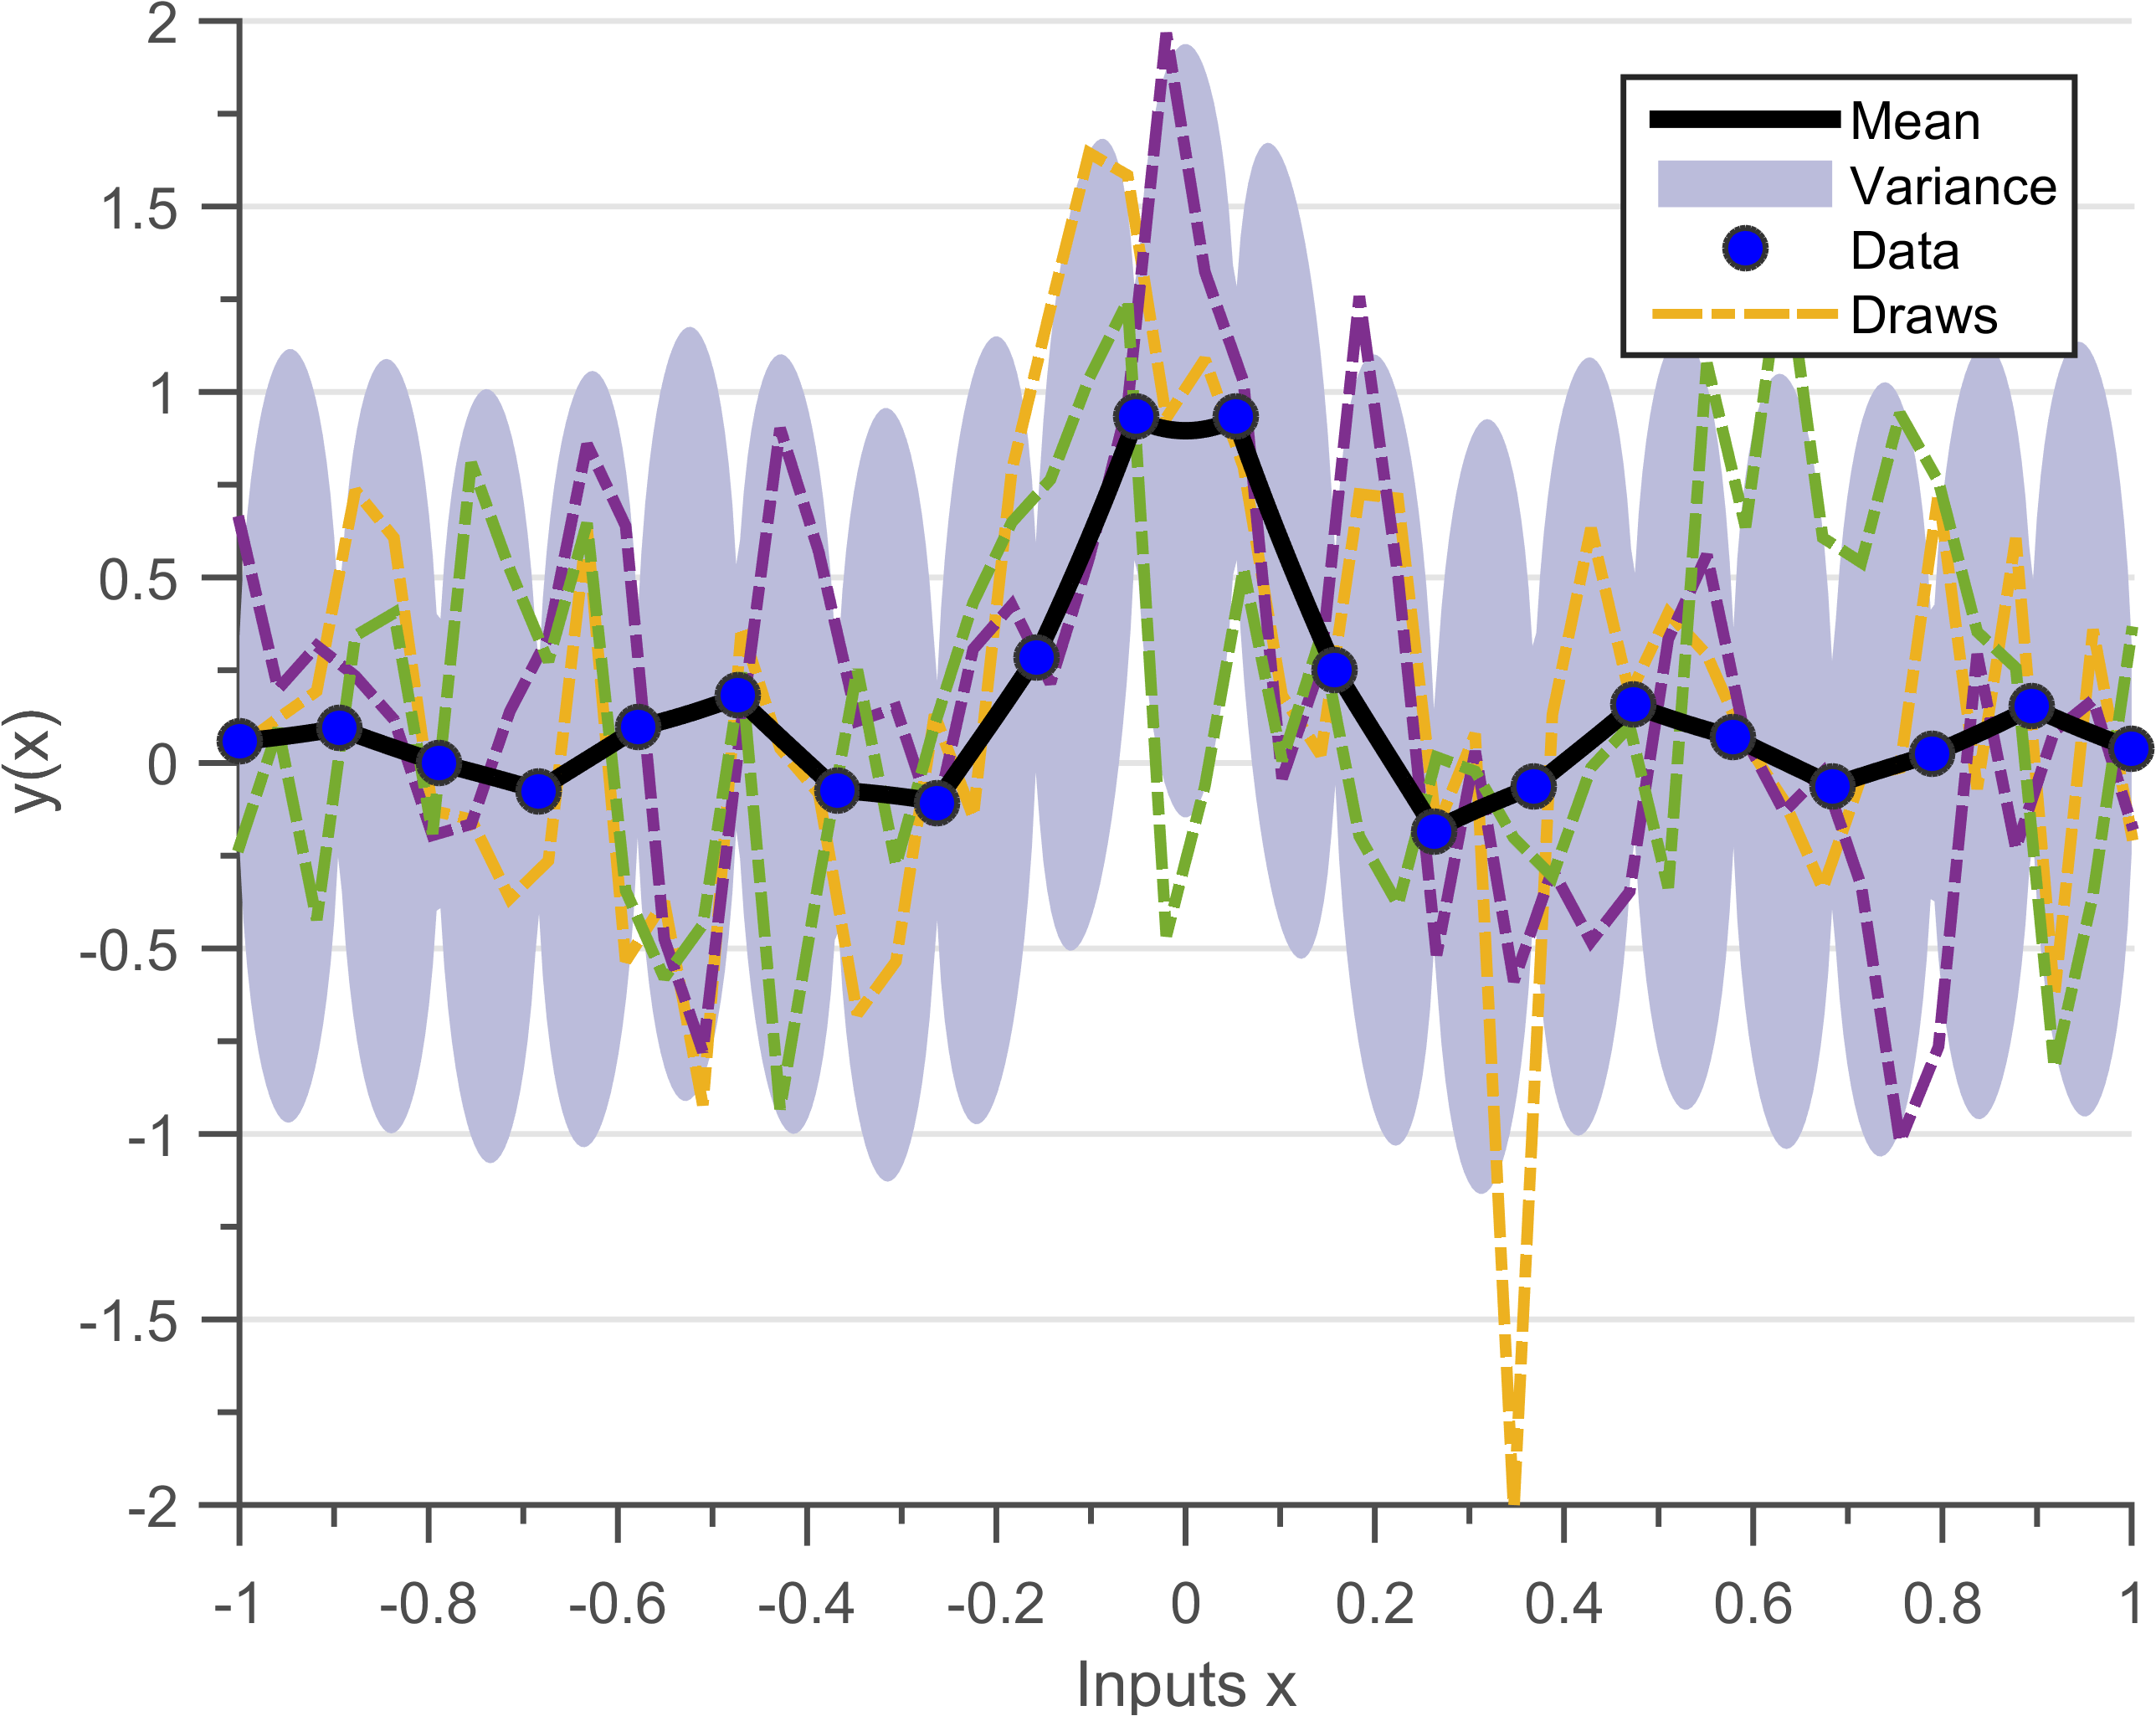
\includegraphics[width=0.29\textwidth]
        {imagesPart2/drawsPosteriorEXP}
        \label{subFigdrawsPosteriorEXP}
  }\quad
\subfigure[{Draws from a GP posterior with mean zero and Mat\'ern kernel \(\nu = 3/2\) (figure \ref{subFigpriorDrawsMAT3}) conditioned on the data \(\mathcal{D}_{2}\). The posterior mean passes through the data points, random functions drawn from this kernel are differentiable only once}]
  {
        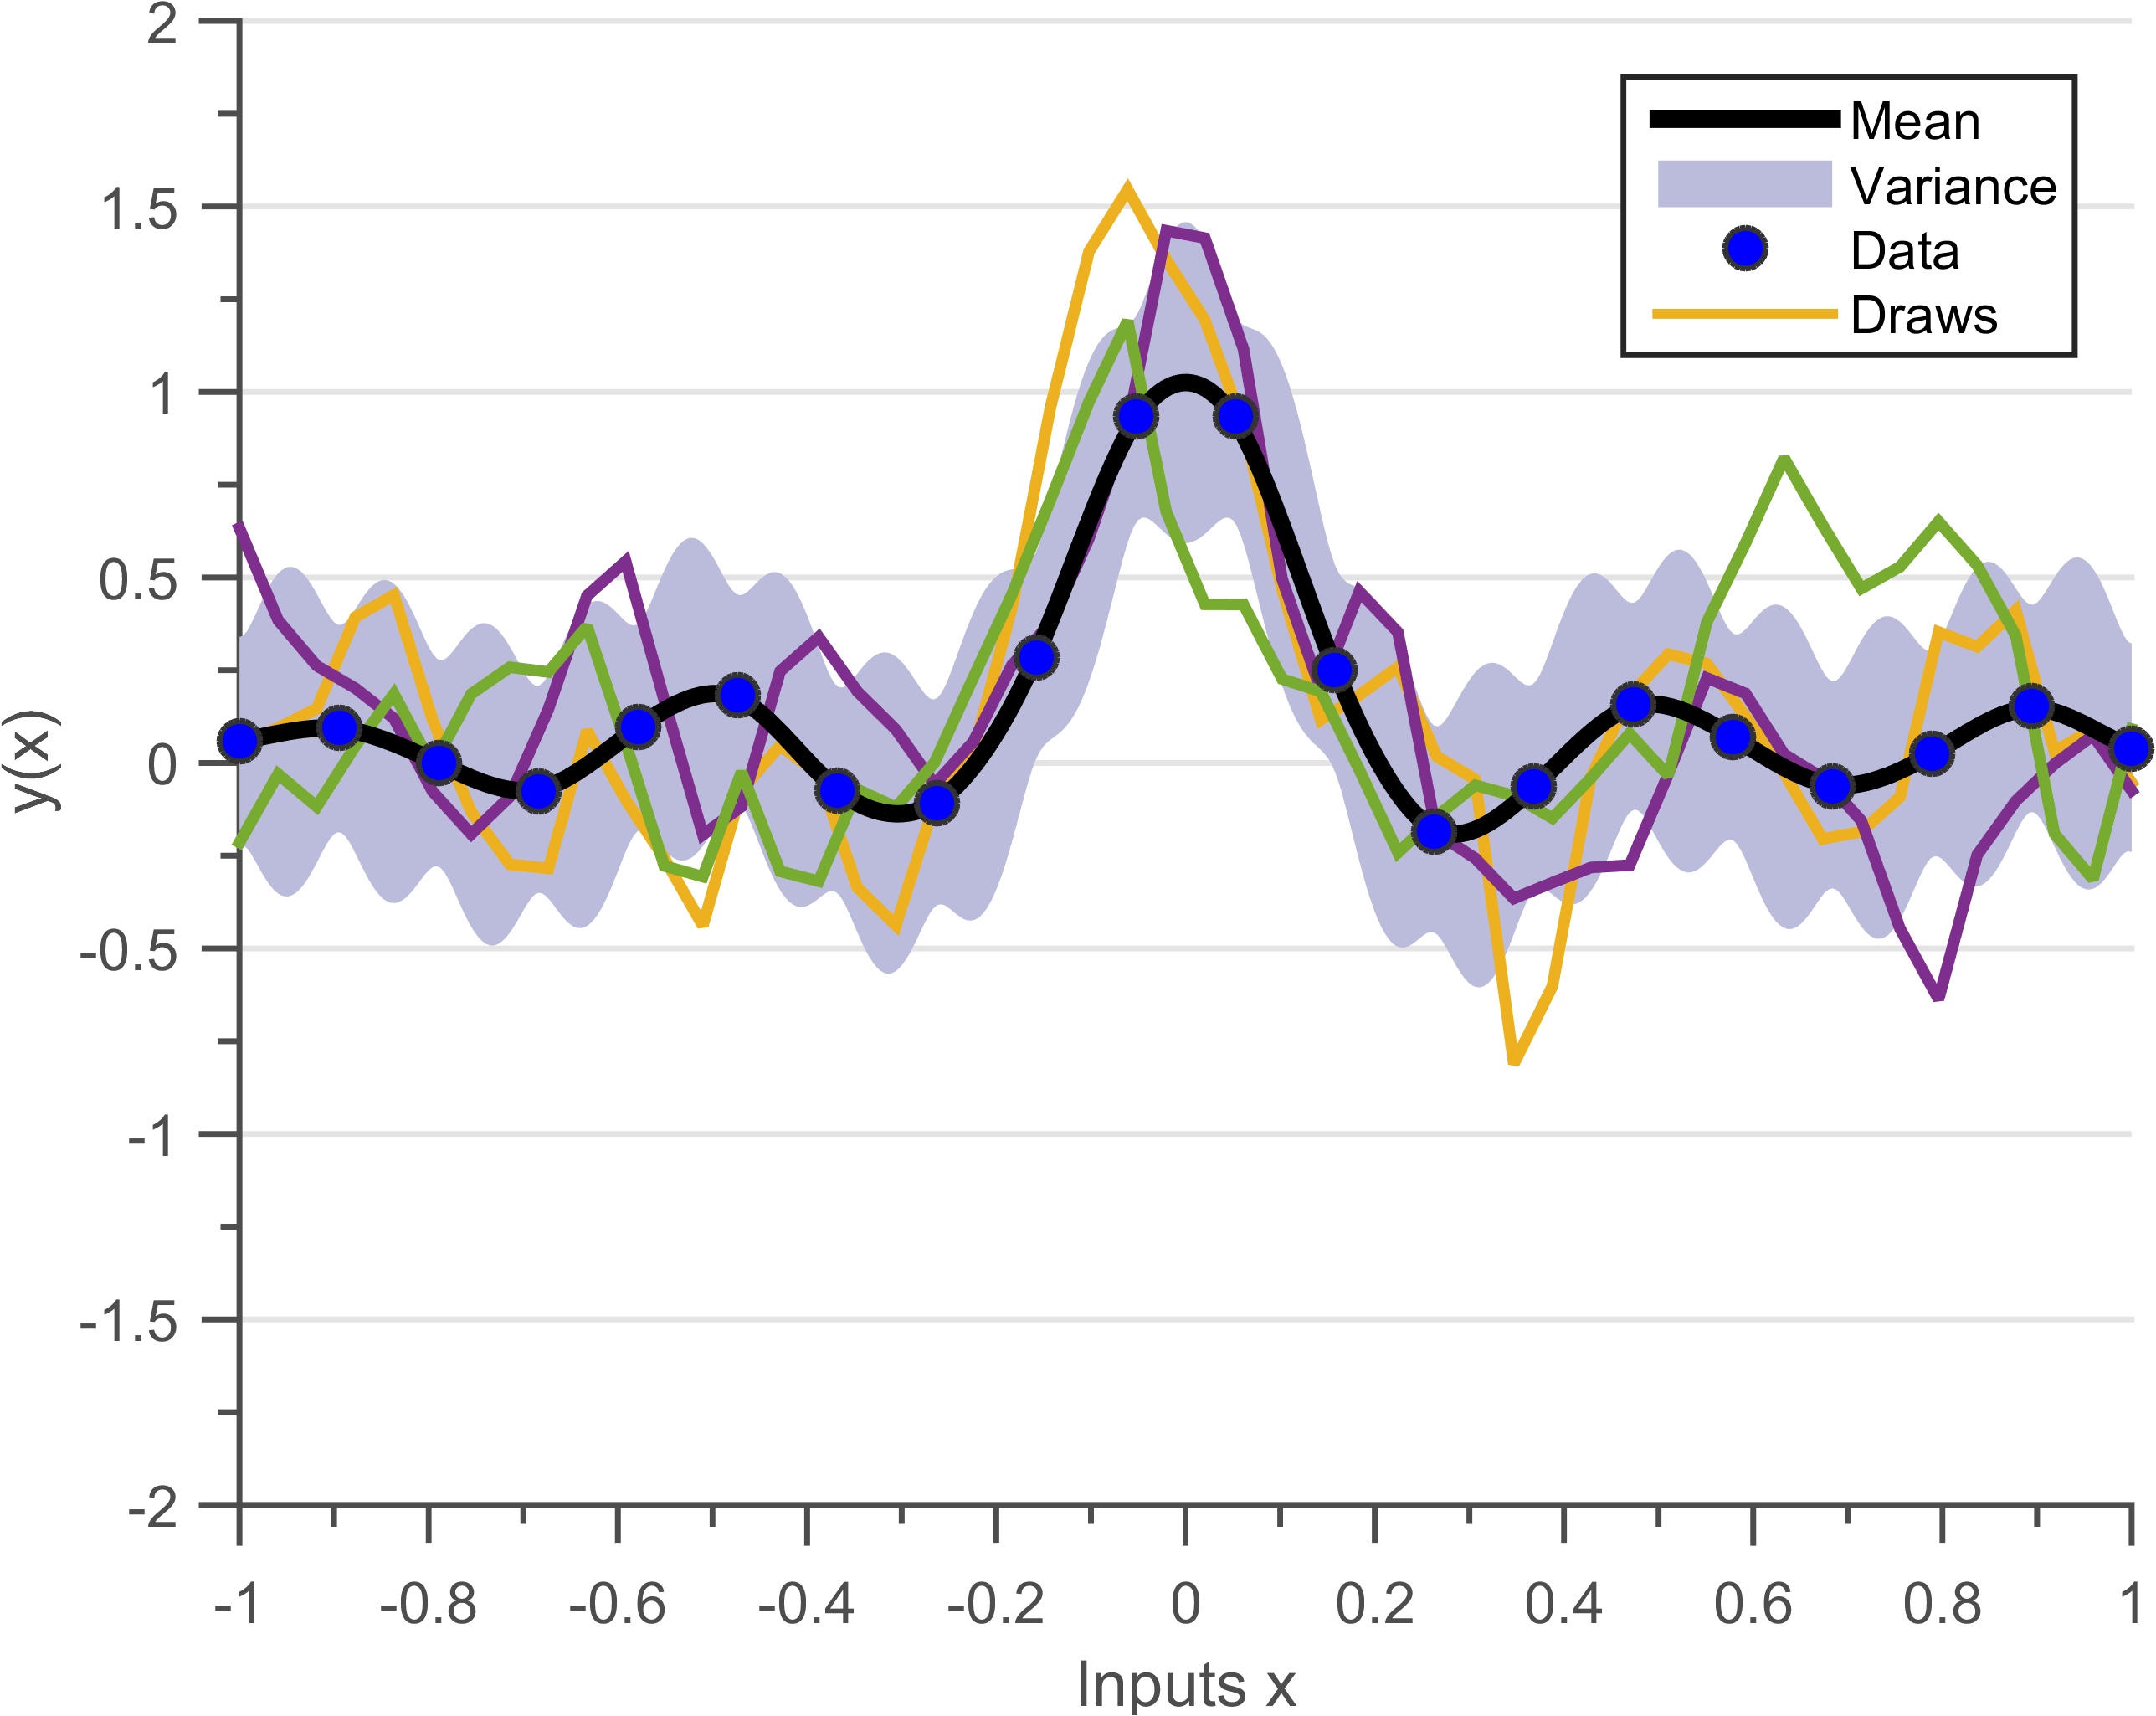
\includegraphics[width=0.29\textwidth]
        {imagesPart2/drawsPosteriorMAT3}
        \label{subFigdrawsPosteriorMAT3}
  }\quad
  \subfigure[{Draws from a GP posterior with mean zero and Standard exponential kernel \(\nu = \infty\) (figure \ref{subFigpriorDrawsMAT3}) conditioned on the data \(\mathcal{D}_{2}\). The posterior mean passes through the data points, random functions drawn from exponential kernel are infinitely differentiable}]
  {
        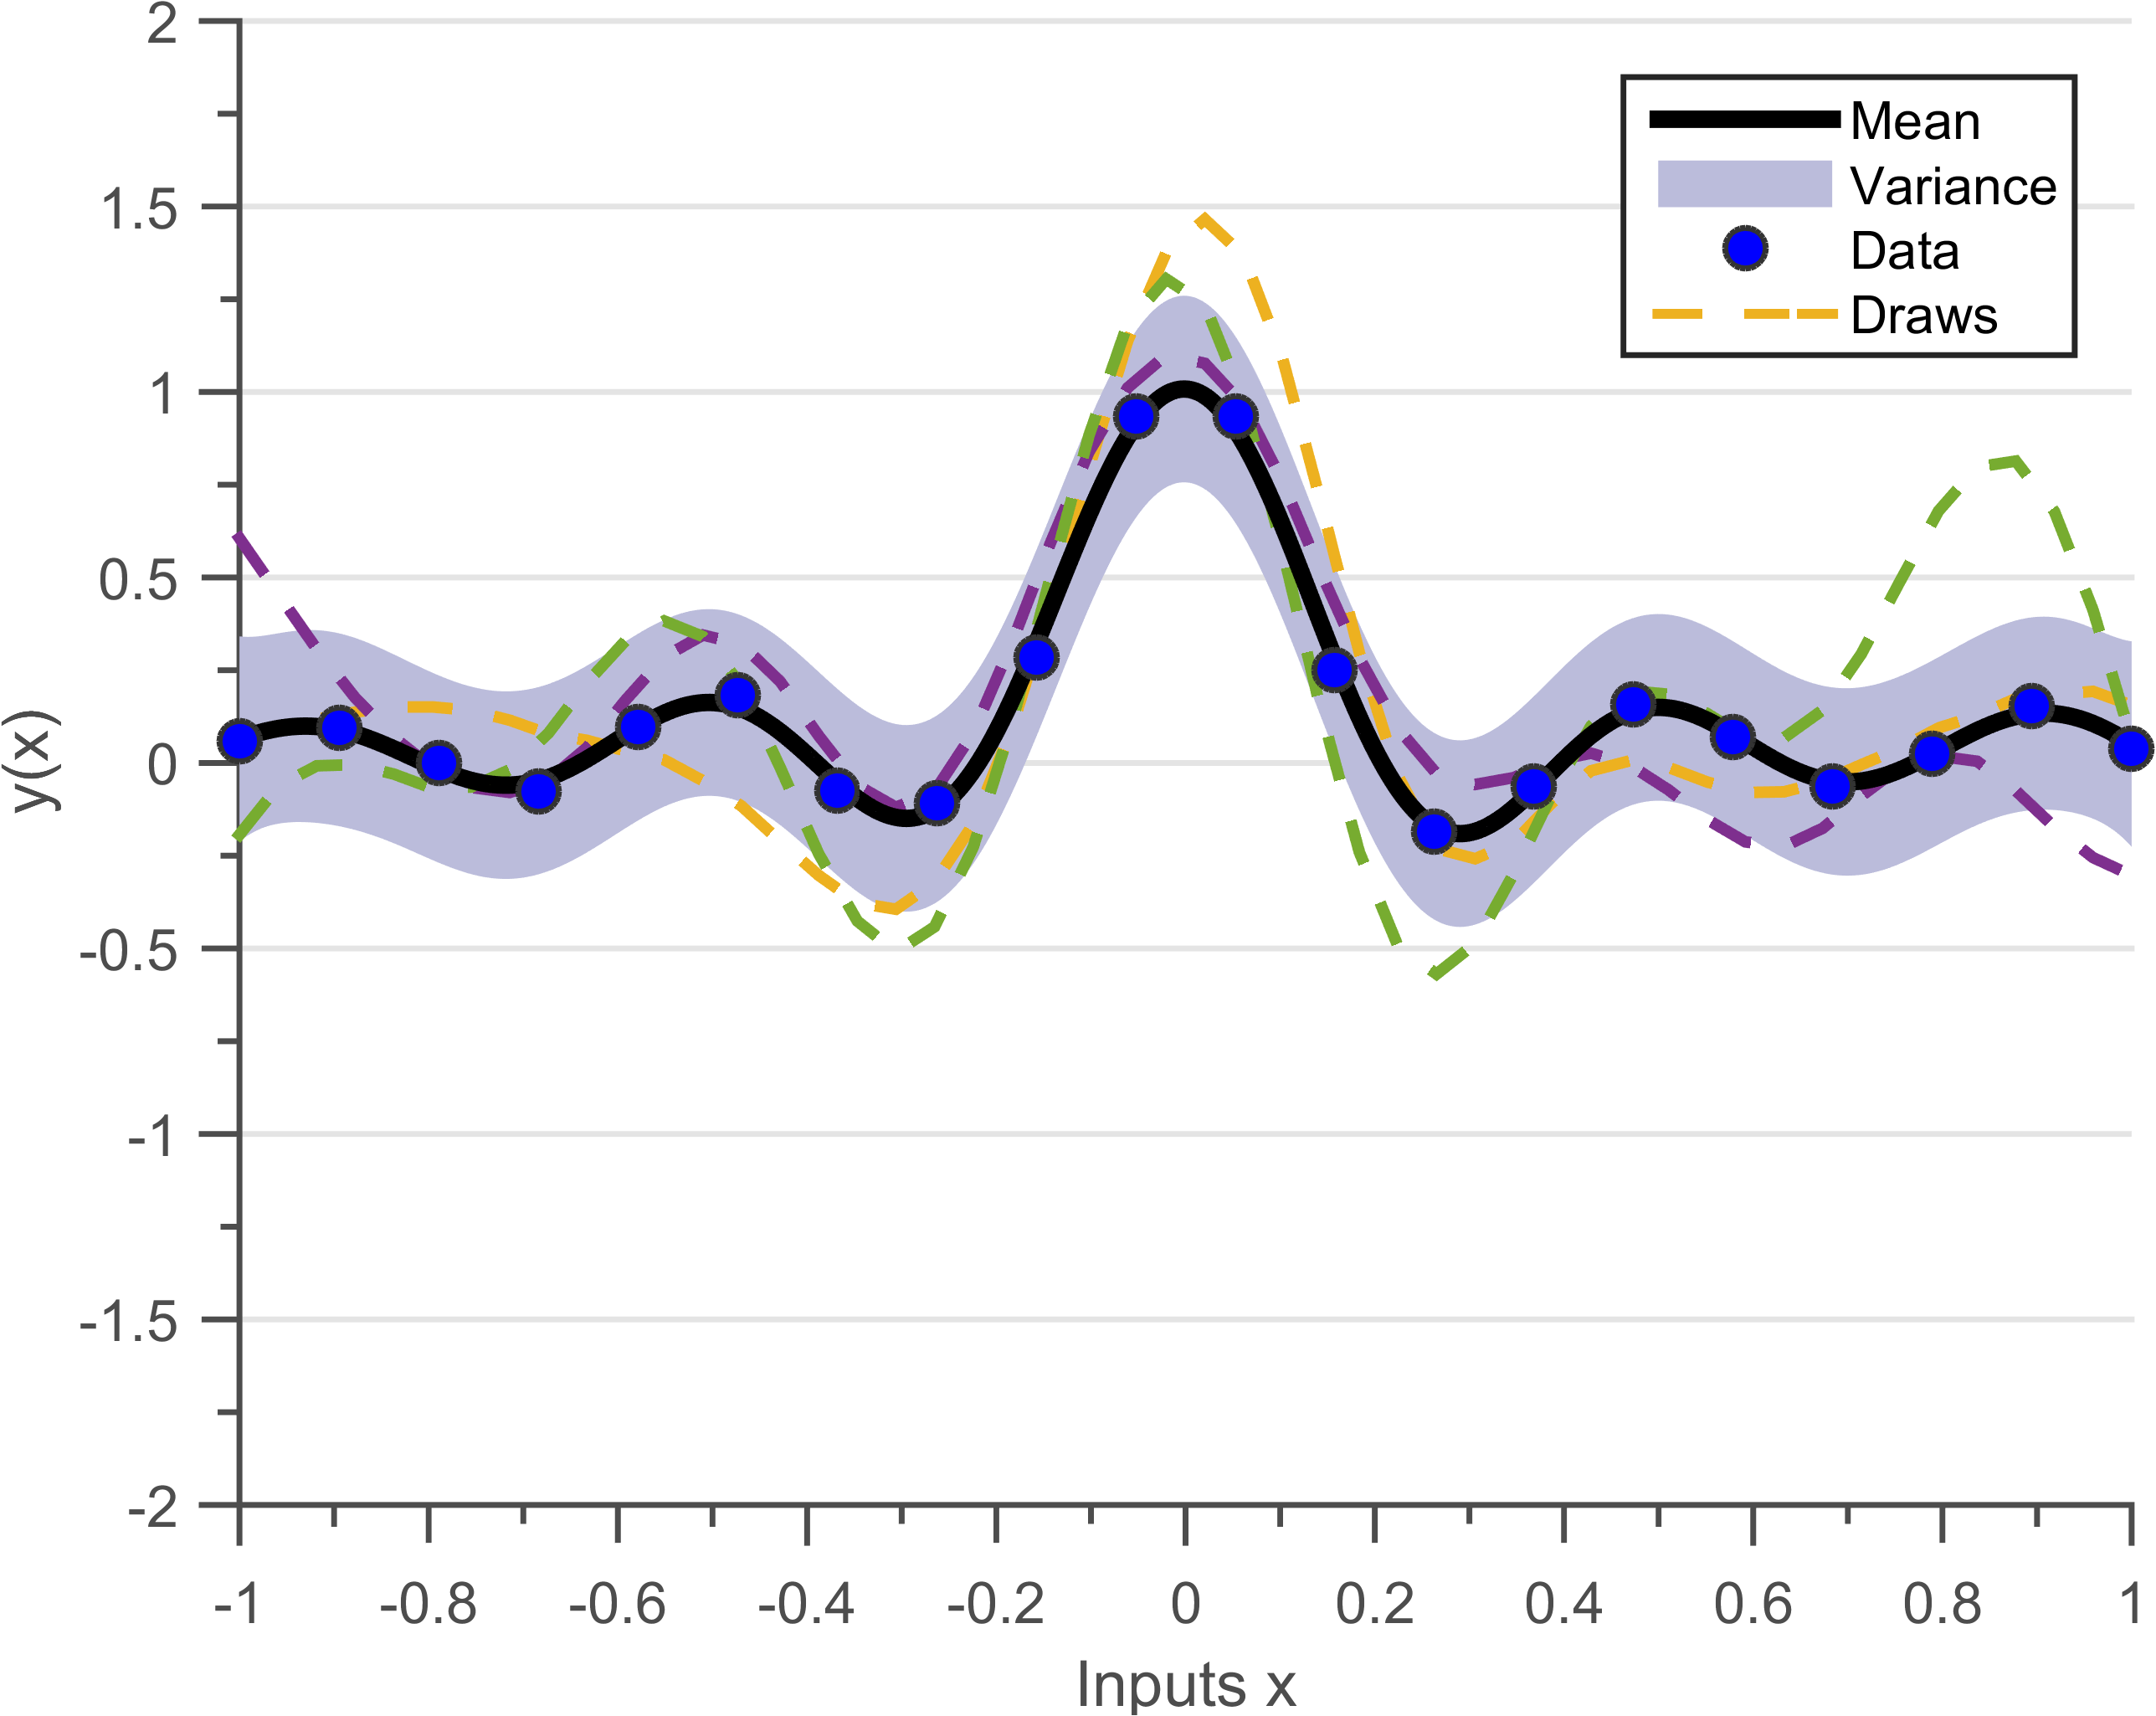
\includegraphics[width=0.29\textwidth]
        {imagesPart2/drawsPosteriorSE}
        \label{subFigdrawsPosteriorSE}
  }\quad
\caption{Posterior distribution and three random draws from 3 different covariance functions. The solid black line defines the mean function, shaded blue region defines 95\% confidence interval (2\(\sigma\)) distance away from the mean. The dashed lines are five functions drawn at random from a GP prior. }
       \label{figpreOptimizedPosteriorCh5}
\end{figure}


Figure \ref{figOptimizedPosteriorCh4} shows the posterior GP conditioned on the dataset \(\mathcal{D}_{2}\) for three different covariance functions with optimized hyper-parameters. This experiment only shows the different posteriors obtained for same observational data and different functional forms of the covariance function. All three predictions can be the correct interpolations depending on the type of experiment, this is where engineering judgment is required. For example, if the dataset \(\mathcal{D}_{2}\) was sampled from a Brownian motion then figure \ref{subFigdrawsOptimizedPosteriorEXP} would be the best fit. 

\begin{figure}[!ht]
  \centering
    \subfigure[{Draws from a GP posterior, conditioned on the dataset \(\mathcal{D}_{1}\) with mean zero and Exponential kernel with hyper-parameters (\(\theta_{lengthscale} = 0.215\), \(\theta_{amplitude} = 0.312\) and \(\sigma_{n} = 2.8e^-5\)) that maximize the marginal likelihood \(max(ML) = -1\).}]
  {
        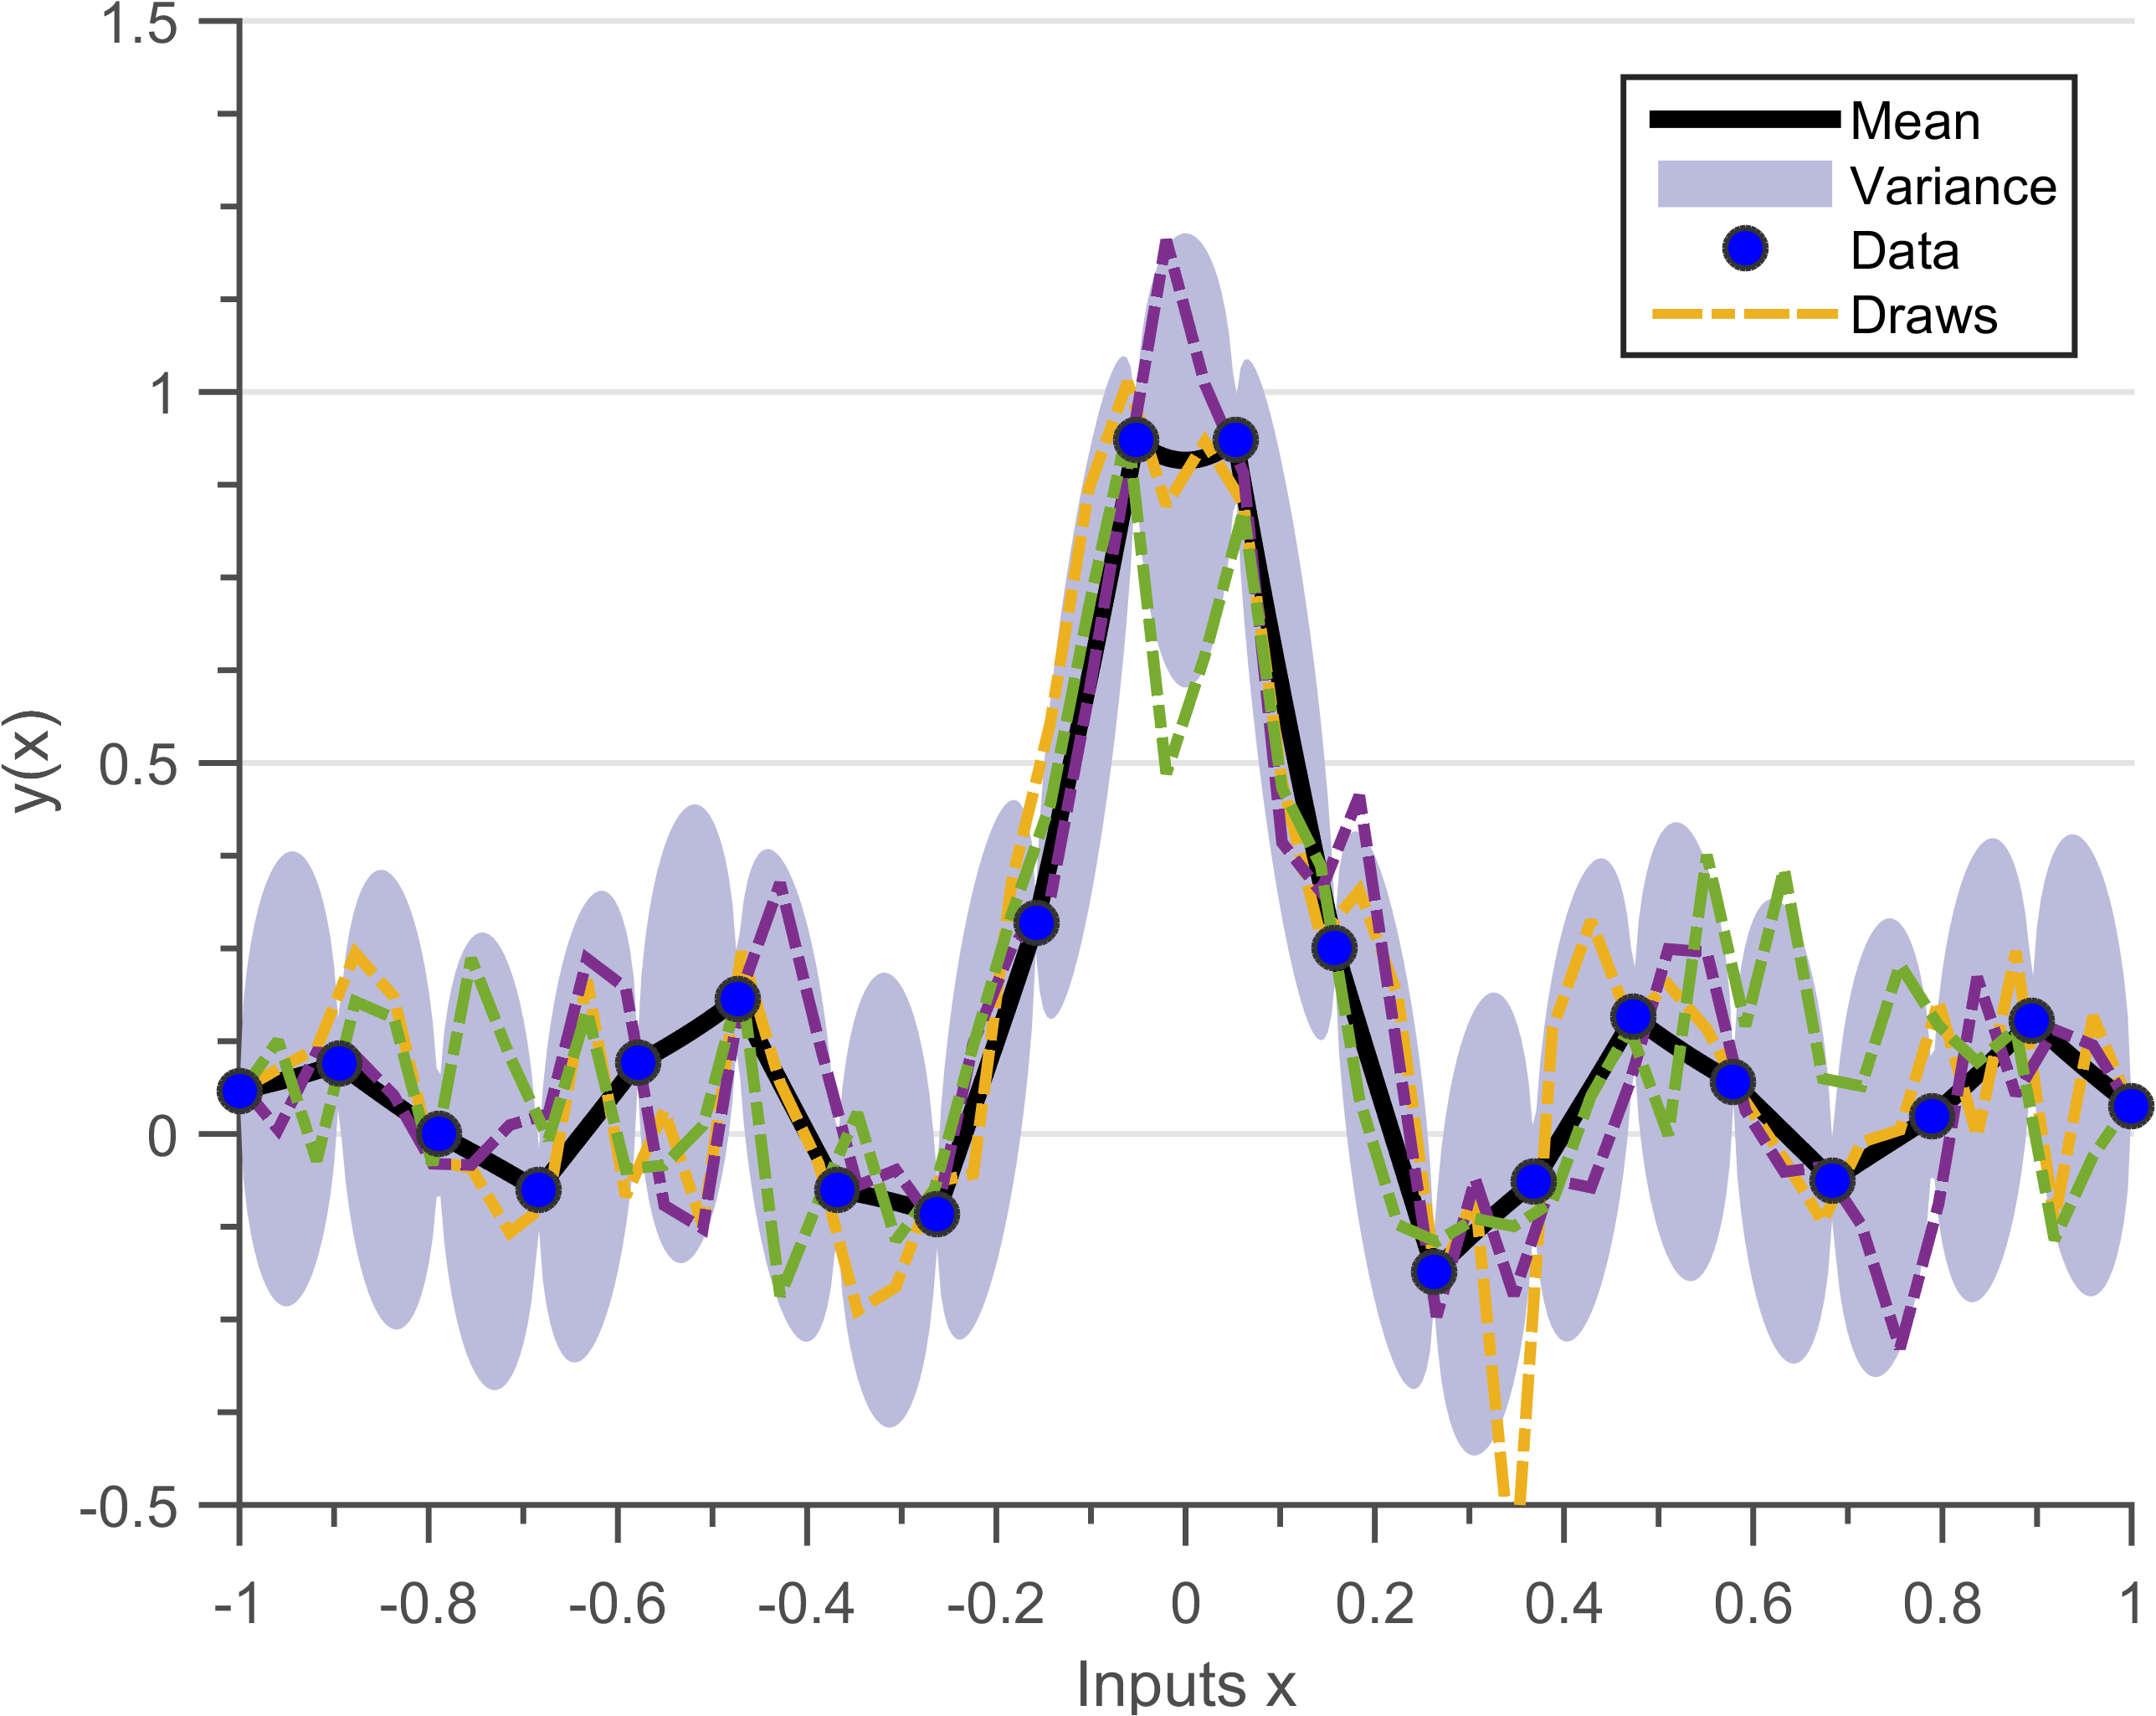
\includegraphics[width=0.29\textwidth]
        {imagesPart2/drawsOptimizedPosteriorEXP}
        \label{subFigdrawsOptimizedPosteriorEXP}
  }\quad
\subfigure[{Draws from a GP posterior, conditioned on the dataset \(\mathcal{D}_{1}\) with mean zero and Mat\'ern (\(\nu=3/2\)) kernel with hyper-parameters (\(\theta_{lengthscale} = 0.2\), \(\theta_{amplitude} = 0.347\) and \(\sigma_{n} = 1.7e^-5\)) that maximize the marginal likelihood \(max(ML) = 2\)}]
  {
        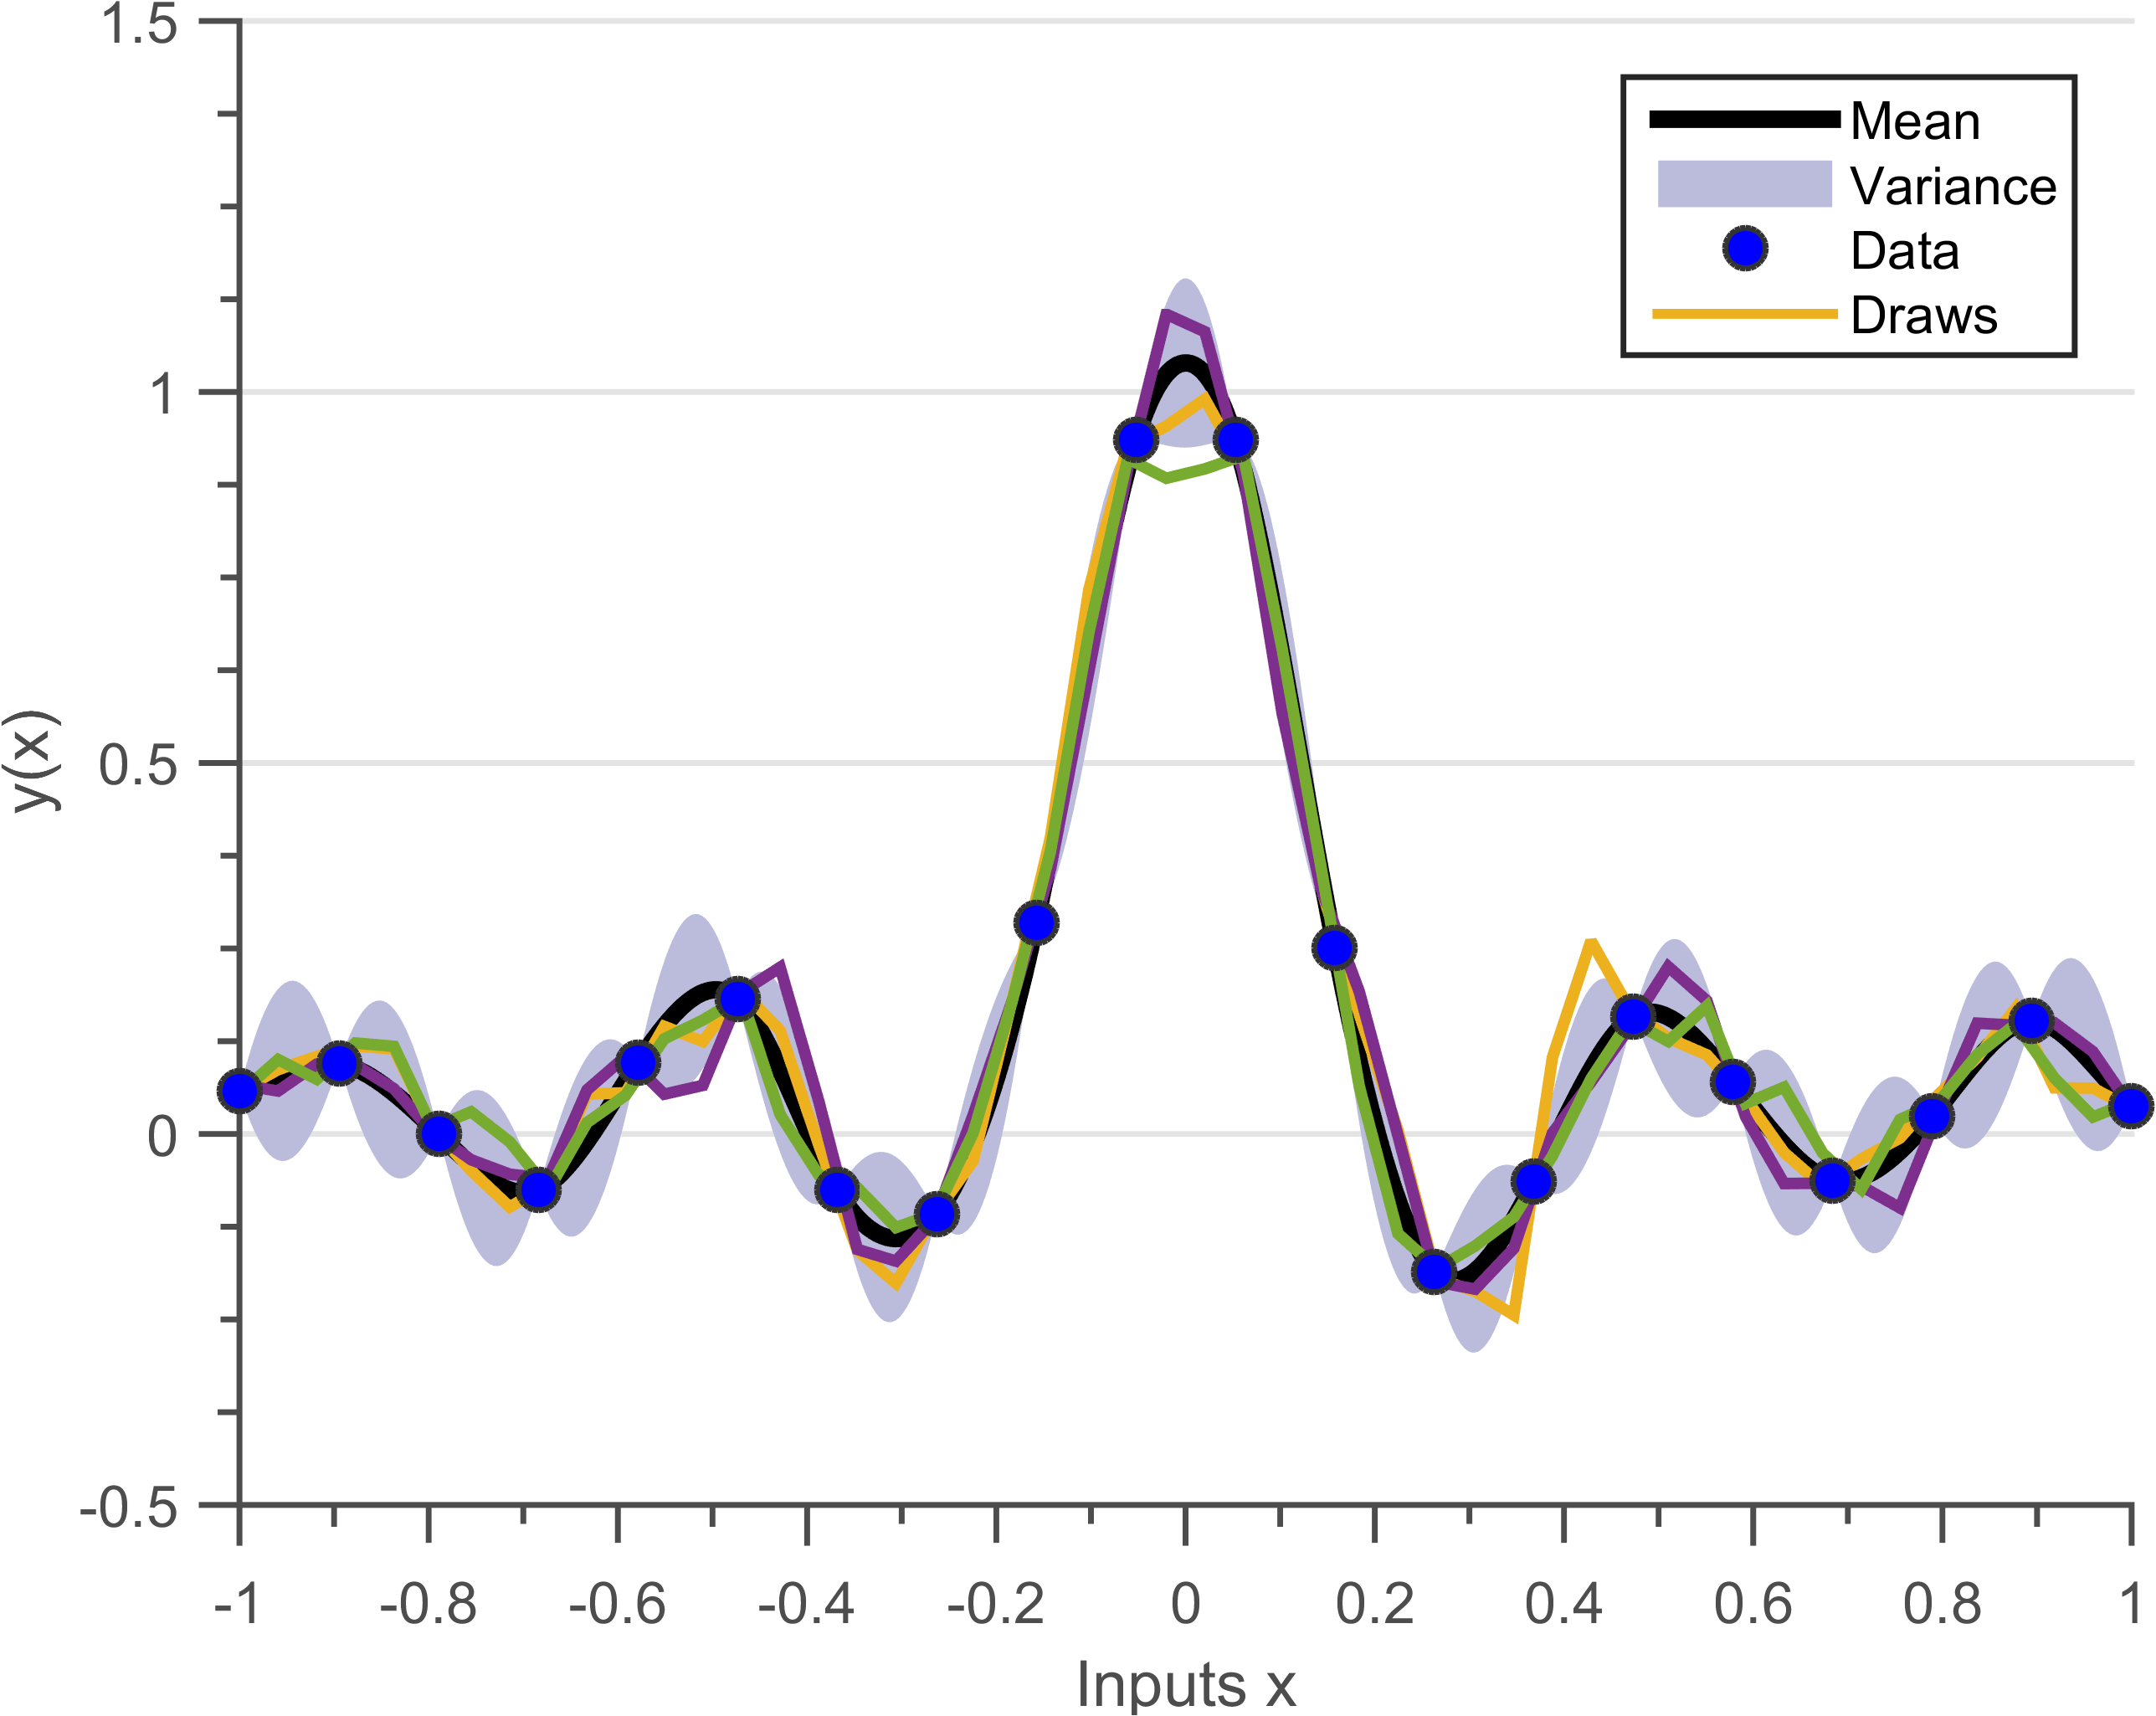
\includegraphics[width=0.29\textwidth]
        {imagesPart2/drawsOptimizedPosteriorMAT3}
        \label{subFigdrawsOptimizedPosteriorMAT3}
  }\quad
  \subfigure[{Draws from a GP posterior, conditioned on the dataset \(\mathcal{D}_{1}\) with mean zero and se kernel with hyper-parameters (\(\theta_{lengthscale} = 0.151\), \(\theta_{amplitude} = 0.358\) and \(\sigma_{n} = 0.01\)) that maximize the marginal likelihood \(max(ML) = 8\)}]
  {
        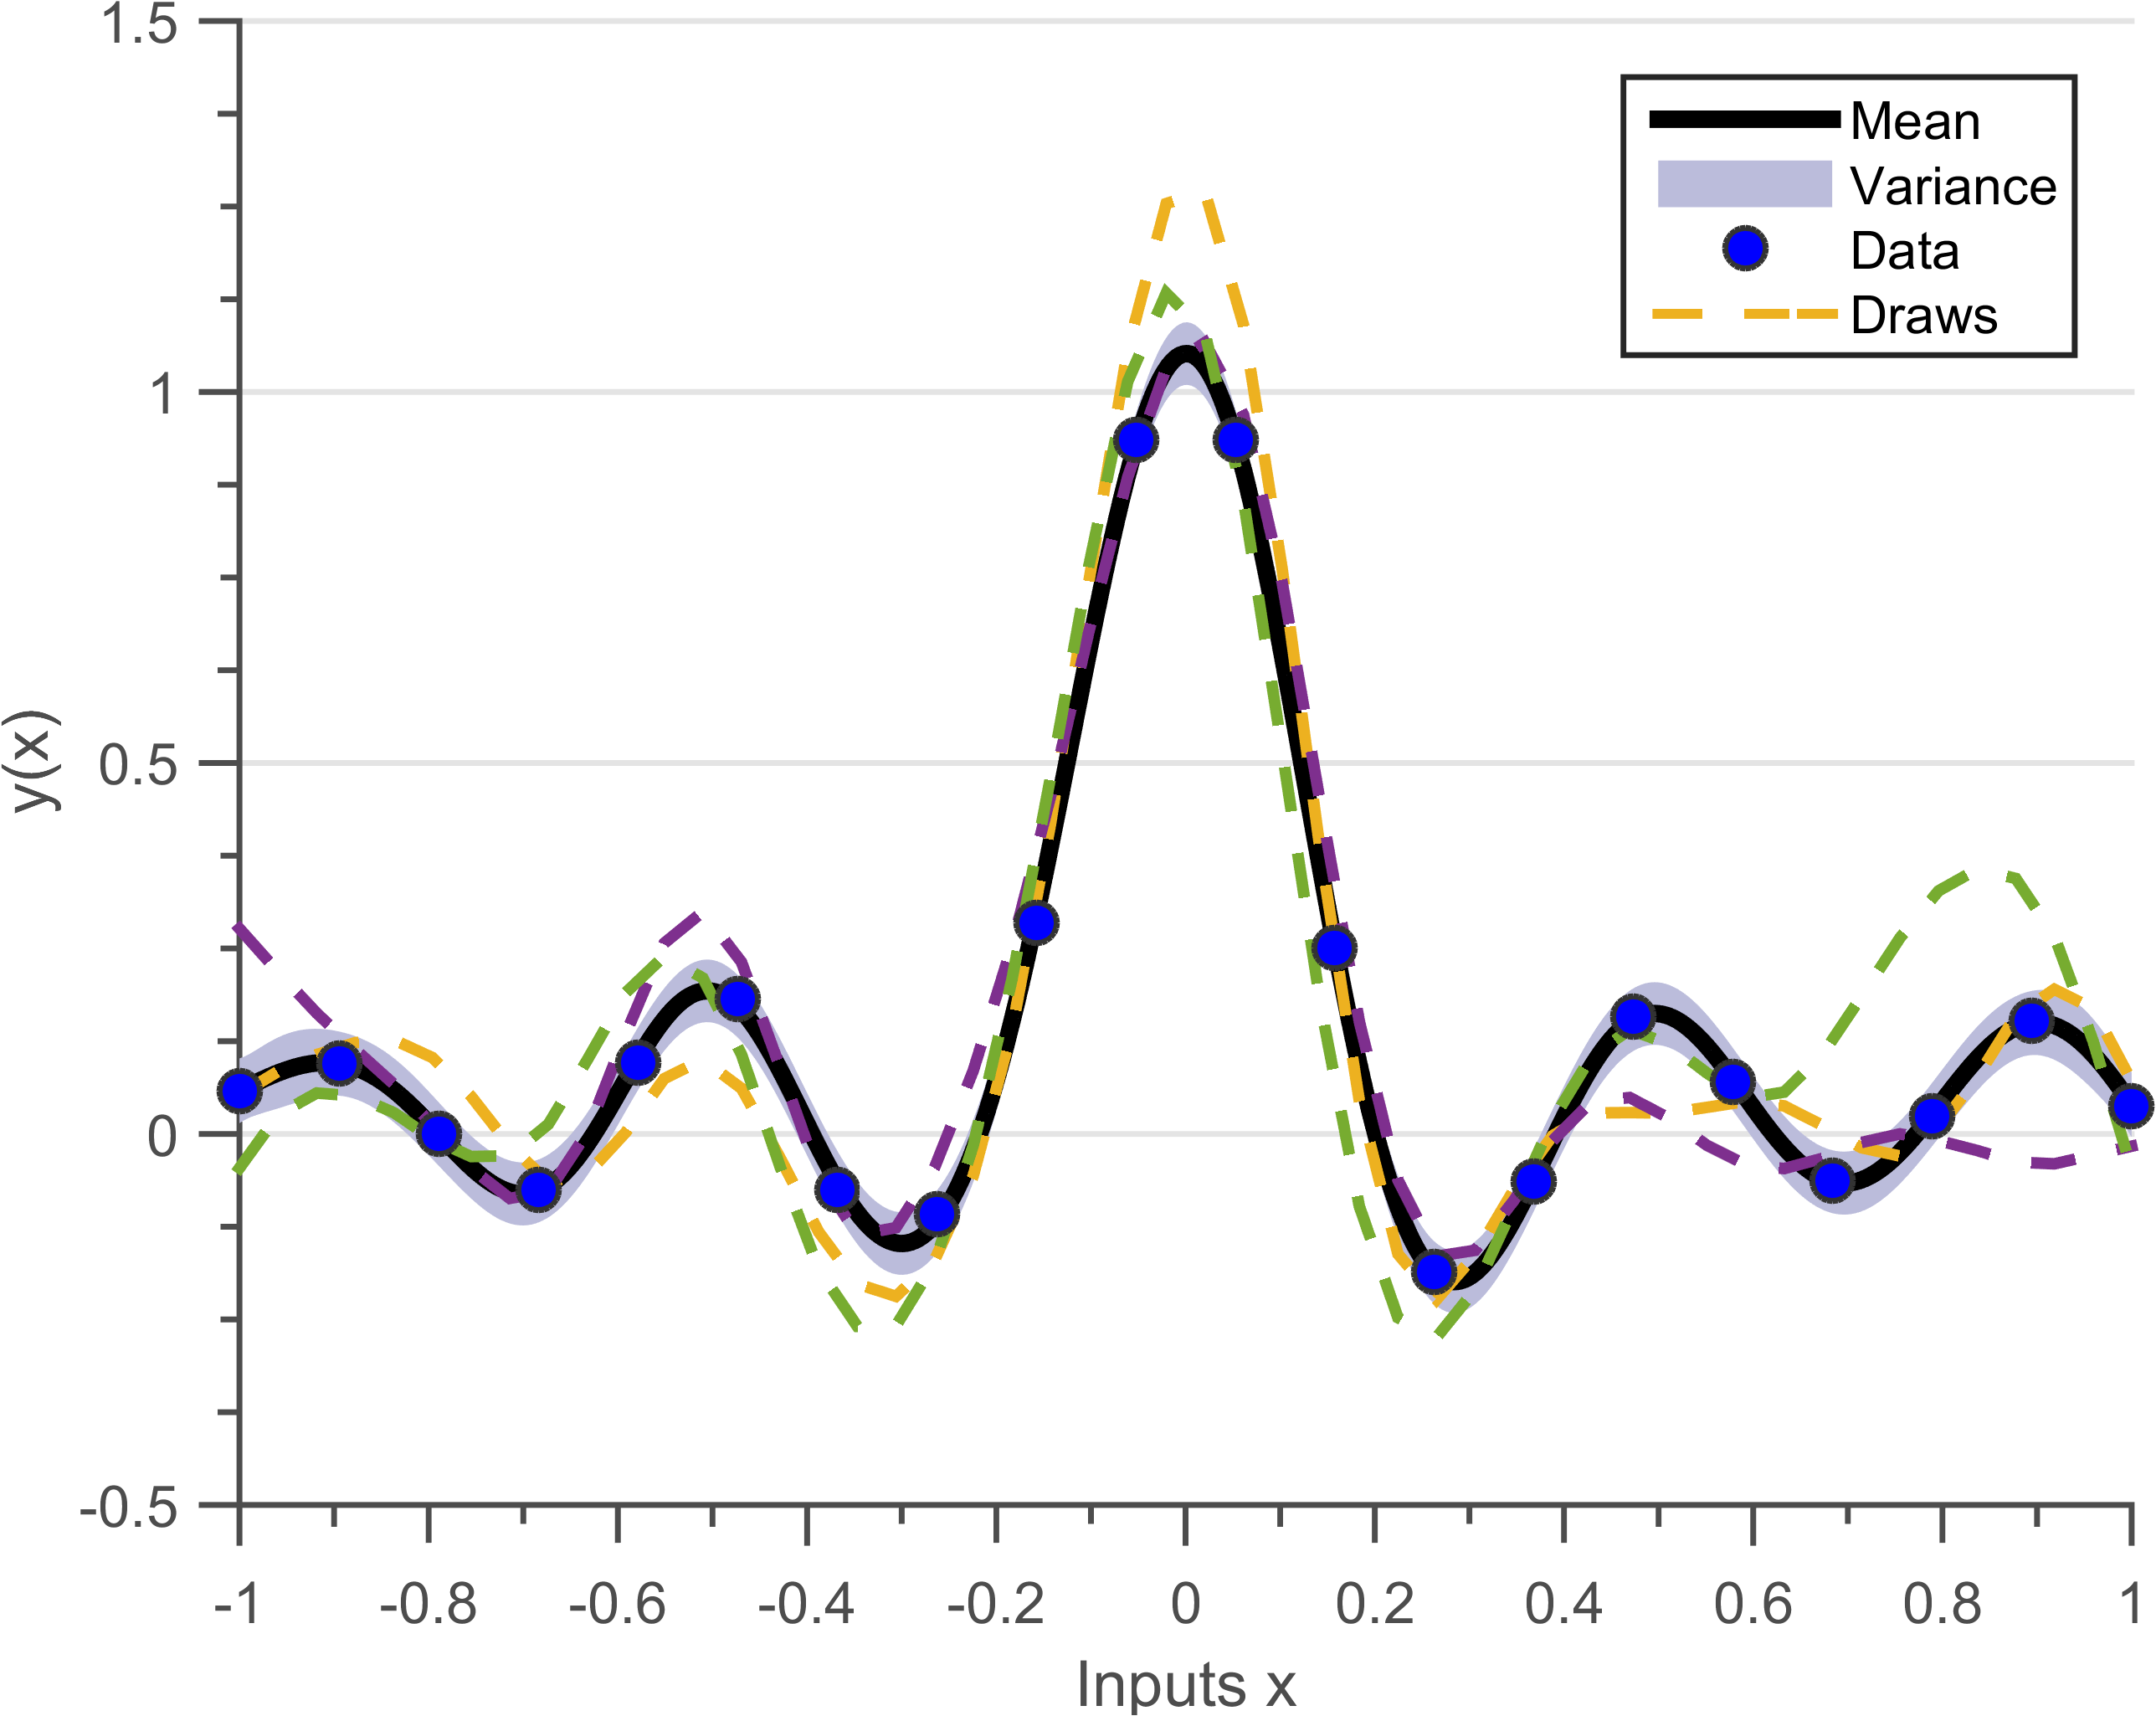
\includegraphics[width=0.29\textwidth]
        {imagesPart2/drawsOptimizedPosteriorSE}
        \label{subFigdrawsOptimizedPosteriorSE}
  }\quad
\caption{Posterior distributions from three different covariance functions after maximizing the hyper-parameters.}
       \label{figOptimizedPosteriorCh4}
\end{figure}

If nothing is known about the data or type of experiment and the number of hyper-parameters are same then the covariance function with the maximum optimized marginal likelihood should be a preferred (By this logic the SE kernel should be preferred functional form of covariance function for dataset \(\mathcal{D}_{2}\)). If number hyper-parameters are not same then marginal likelihood tends to be higher for covariance functions with greater number of hyper-parameters. \cite{duvenaud-thesis-2014, lloyd2014automatic} propose to use the Bayesian Information Criteria (equation \ref{eq:BIC}) to choose optimal covariance functions if number of hyper-parameters are not same. 

\subsection{Spectral Mixture Kernels}\label{subSecSMKernel}
Spectral mixture kernels define a more general class of stationary kernels exploiting the Bochner's theorem \cite{bochner1959lectures}. They define the power spectrum as a scale location mixture of Gaussians \cite{wilson2013gaussian}. This has two benefits firstly, with enough Gaussian components, scale location mixtures of Gaussians can approximate a curve up to arbitrary precision\cite{kostantinos2000gaussian, bishop2006pattern}. Secondly, the inverse Fourier transform of a Scale location mixture of Gaussians is analytically tractable and is also a mixture of Gaussians.

\begin{equation}\label{eqPowerSpectrumSSM}
    S_{SM}(s, \mu, \sigma, w) = \sum_{q=1}^{Q} \frac{w_{q}}{\sqrt{2\pi\sigma_{q}^2}}
\left ( \exp\left [ {-\frac{{(s-\mu_{q})^2}}{2\sigma_{q}^{2}}} \right ] + \exp\left [ {-\frac{{(-s-\mu_{q})^2}}{2\sigma_{q}^{2}}} \right ] \right  )
\end{equation}

Here, \( S_{SM}\) is the power spectrum of the spectral mixture kernel. Each Gaussian  component \(q\) has a mean \(\mu_{q}\), variance \(\sigma_{q}\) and weight \(w_{q}\) , there are total \(Q\) such components. The second term \(\exp\left [ {-\frac{{(-s-\mu_{q})^2}}{2\sigma_{q}^{2}}} \right ]\) is needed because a power spectrum of a valid kernels should be symmetric around \(s=0\). The inverse Fourier transform of such a power spectrum will be a valid kernel and can be written as below, for a detailed derivation refer to \cite{wilson2014thesis}.

\begin{equation}\label{eqCovarianceKSM}
k_{SM}(\tau, \mu, \sigma, w) = \sum_{q=1}^{Q}w_{q}cos(2\pi\mu_{q}) exp[-2\pi^{2}\tau^{2}\sigma_{q}^2]
\end{equation}

Here, \(k_{SM}\) is the covariance function of the above power spectrum (equation \ref{eqPowerSpectrumSSM}). The parameter \(w_{q}\) is the weight of the Gaussian component \(q\), the mean of the Gaussian component \(\mu_{q}\) defines the period of kernel while the variance \(\sigma_{q}\) of the Gaussian component denotes inverse of the inverse length scale . Spectral mixture kernels are easily interpretable and can be used as a replacement to many available basic kernels. They can be used to perform pattern discovery, infer negative covariances and perform extrapolation \cite{wilson2014thesis}. 

Although there do exist various other types of basic stationary kernels; for example Gibbs kernel, Rational Quadratic kernel, Periodic kernel etc we mention here only a small quantity of stationary kernels, for more detailed list please refer to work from \cite{Rasmussen2005, duvenaud2013structure, wilson2014thesis}.

Dynamic engineering systems are generally, parametrized by their modal frequencies and participation factors. In structural engineering identification of modal frequencies is an important step for certification, while minor change in modal frequencies can help in speedy discovery of failure. In the next section we apply the Spectral Mixture kernel to identify the modal frequencies of a structural system, parts of the following work have been published in \cite{chiplunkar2017operational}.

\subsection{Application: Identifying Structural Dynamics Parameters}\label{subSecSMKernelApplication}
Modal analysis has been widely used as a means of identifying dynamic properties such as modal frequencies, damping ratios and mode shapes of a structural system. Traditionally, the system is subjected to artificial input excitations and output deformations (displacements, velocities or accelerations) are measured. These later help in identifying the modal parameters of the system, this process is called Experimental Modal Analysis (EMA). 

Since the last decade Operational Modal Analysis (OMA) has gained considerable interest in the community. OMA identifies the modal parameters only from the output measurements while assuming ambient excitations as random noise. OMA is cheaper because it does not require expensive experimental setup and and can be used in real time operational use cases such as health monitoring \cite{peeters2005industrial, shahdin2010correlating, rainieri2007automated}. 

As stated earlier the operational modal analysis is an output dependent modal identification technique. The only thing required is the measurement from the accelerometers placed on the structure. Figure \ref{subfig:randomOutput} shows an example of ambient measurements \(x(t)\) on a structure.  In almost all OMA algorithms the measurement \(x(t)\) is assumed to be generated from a random force excitation. 

In the last few decades several algorithms primarily using the assumption of second order differential, Multi Degree Of Freedom (MDOF) system (equation \ref{eq:secondOrderSystem}) have been developed to find modal parameters in \cite{guillaume2003poly, richardson1982parameter}.

\begin{equation}\label{eq:secondOrderSystem}
    [M]\{\ddot{x}(t)\} + [C]\{\dot{x}(t)\} + [K]\{x(t)\} = \{f(t)\}
\end{equation}

Here, \([M]\), \([C]\) and \([K]\) denote the mass, damping and stiffness matrices respectively. While, \(\{x(t)\}\) and \(\{f(t)\}\) denote the displacement and force vectors at the time \(t\). The Natural Excitation Technique \cite{james1995natural} proves that the auto-correlation function \(k(\tau)\) can be written as sum of decaying sinusoid's \cite{spitznogle1970representation, ibrahim1977method, guillaume2003poly}. The auto-correlation describes the similarity between measurement as a function of time lag \(\tau\) between them figure \ref{subfig:autocorrelationOutput}.  

\begin{equation}\label{eq:NeXT}
    k(\tau) = \int x(t)x(t-\tau)dt \quad k(\tau) = \sum A_{i}exp(-\lambda_{i}\tau)sin(B_{i}\tau)
\end{equation}

Here, \(k(\tau)\) denotes the auto-correlation for random vector \(x(t)\) as a function of time lag \(\tau\). Here, \(\lambda_{i}\) and \(A_{i}\) denotes the modal frequency and mode shapes for the \(i^{th}\) mode. The above coefficients are found by minimizing the least square error between the measured \(k(\tau)\) and the predicted \(k(\tau)\) from equation \ref{eq:NeXT}

If we assume the measurement \(x(t)\) to be a stationary random process, then according to Bochner's theorem the Fourier transform of \(k(\tau)\) (power spectrum \(S(s)\)) exists \cite{bochner2016lectures}. Figure \ref{subfig:psdOutput} shows the power spectrum calculated for the measurement \(x(t)\) shown in figure \ref{subfig:randomOutput}. Using the above mentioned second order differential equation assumption a Rational Fractional Polynomial (equation \ref{eq:RFP}) can be used to fit a power spectrum \cite{richardson1982parameter, allemang1998unified, chauhan2007unified}.

\begin{equation}\label{eq:RFP}
S(s) = \int k(\tau) e^{-2 \pi is^{T} s}d\tau \quad    S(s) = \frac{\sum a_{k}(s)^{k}}{\sum b_{l}(s)^{l}}
\end{equation}

Here, the poles of the polynomial denote the modal frequencies, while other modal parameters can be derived from the coefficients \(a_{k}\) and \(b_{l}\). The coefficients of the polynomial can be found by minimizing the least squared error. RFP based algorithms face problems since as the number of modes increase the matrix becomes ill-conditioned which gives rise to stability issues in prediction of modal parameters. In the next section we will drop the assumption of second order differential system and treat the modal identification as a purely curve-fitting problem.

Two of the above mentioned OMA algorithms ``Natural Excitation Technique" in the time lag (\( \tau\))domain and ``Rational Fractional Polynomial" in the frequency domain \(s\), have a core assumption of second order differential system. This assumption fails for non-linear systems and for cases where modal frequencies are very close. Instead we propose the spectral mixture kernel to fit the measurement \(x(t)\). 

Using the same hypothesis used in section \ref{subSecSMKernel}, we can say that a scale-location mixture of Gaussian components can approximate any distribution. We thus place a Gaussian Mixture Model (GMM) on the power spectrum (\(S(s)\)), this means that we are assuming a prior distribution of \(x(t)\) as a Gaussian Process with a Spectral Mixture kernel (equation \ref{eqTimeFitting}). The hyper-parameters of the system are: the mean \(\mu_{q}\) defines the modal frequency, the variance \(\sigma_{q}\) which is a measure of damping, the weight \(w_{q}\) which defines the participation factor of component \(q\) and the total number of components \(Q\).

\begin{equation}\label{eqTimeFitting}
\Pr[x(t)] = GP(0, k_{SM} = \sum_{q=1}^{Q}w_{q}cos(2\pi\mu_{q}) exp[-2\pi^{2}\tau^{2}\sigma_{q}^2)
\end{equation}

We would like to emphasize that keeping the computational complexities aside, fitting a Spectral Mixture GP in time-domain equation \ref{eqTimeFitting}, fitting equation \ref{eqCovarianceKSM} for covariance identification and fitting a GMM equation \ref{eqPowerSpectrumSSM} in the frequency-domain are equivalent. In the publication \cite{chiplunkar2017operational} we fit a GMM on the frequency domain, here we propose to fit the GP on the measurements \(x(t)\) . Refer to table \ref{tab:comparisonOfFittingFunctions} for a more comprehensive view at various fitting functions.

\begin{figure*}[!ht]
  \centering
  \subfigure[Measured output on accelerometers \(x(t)\)]
  {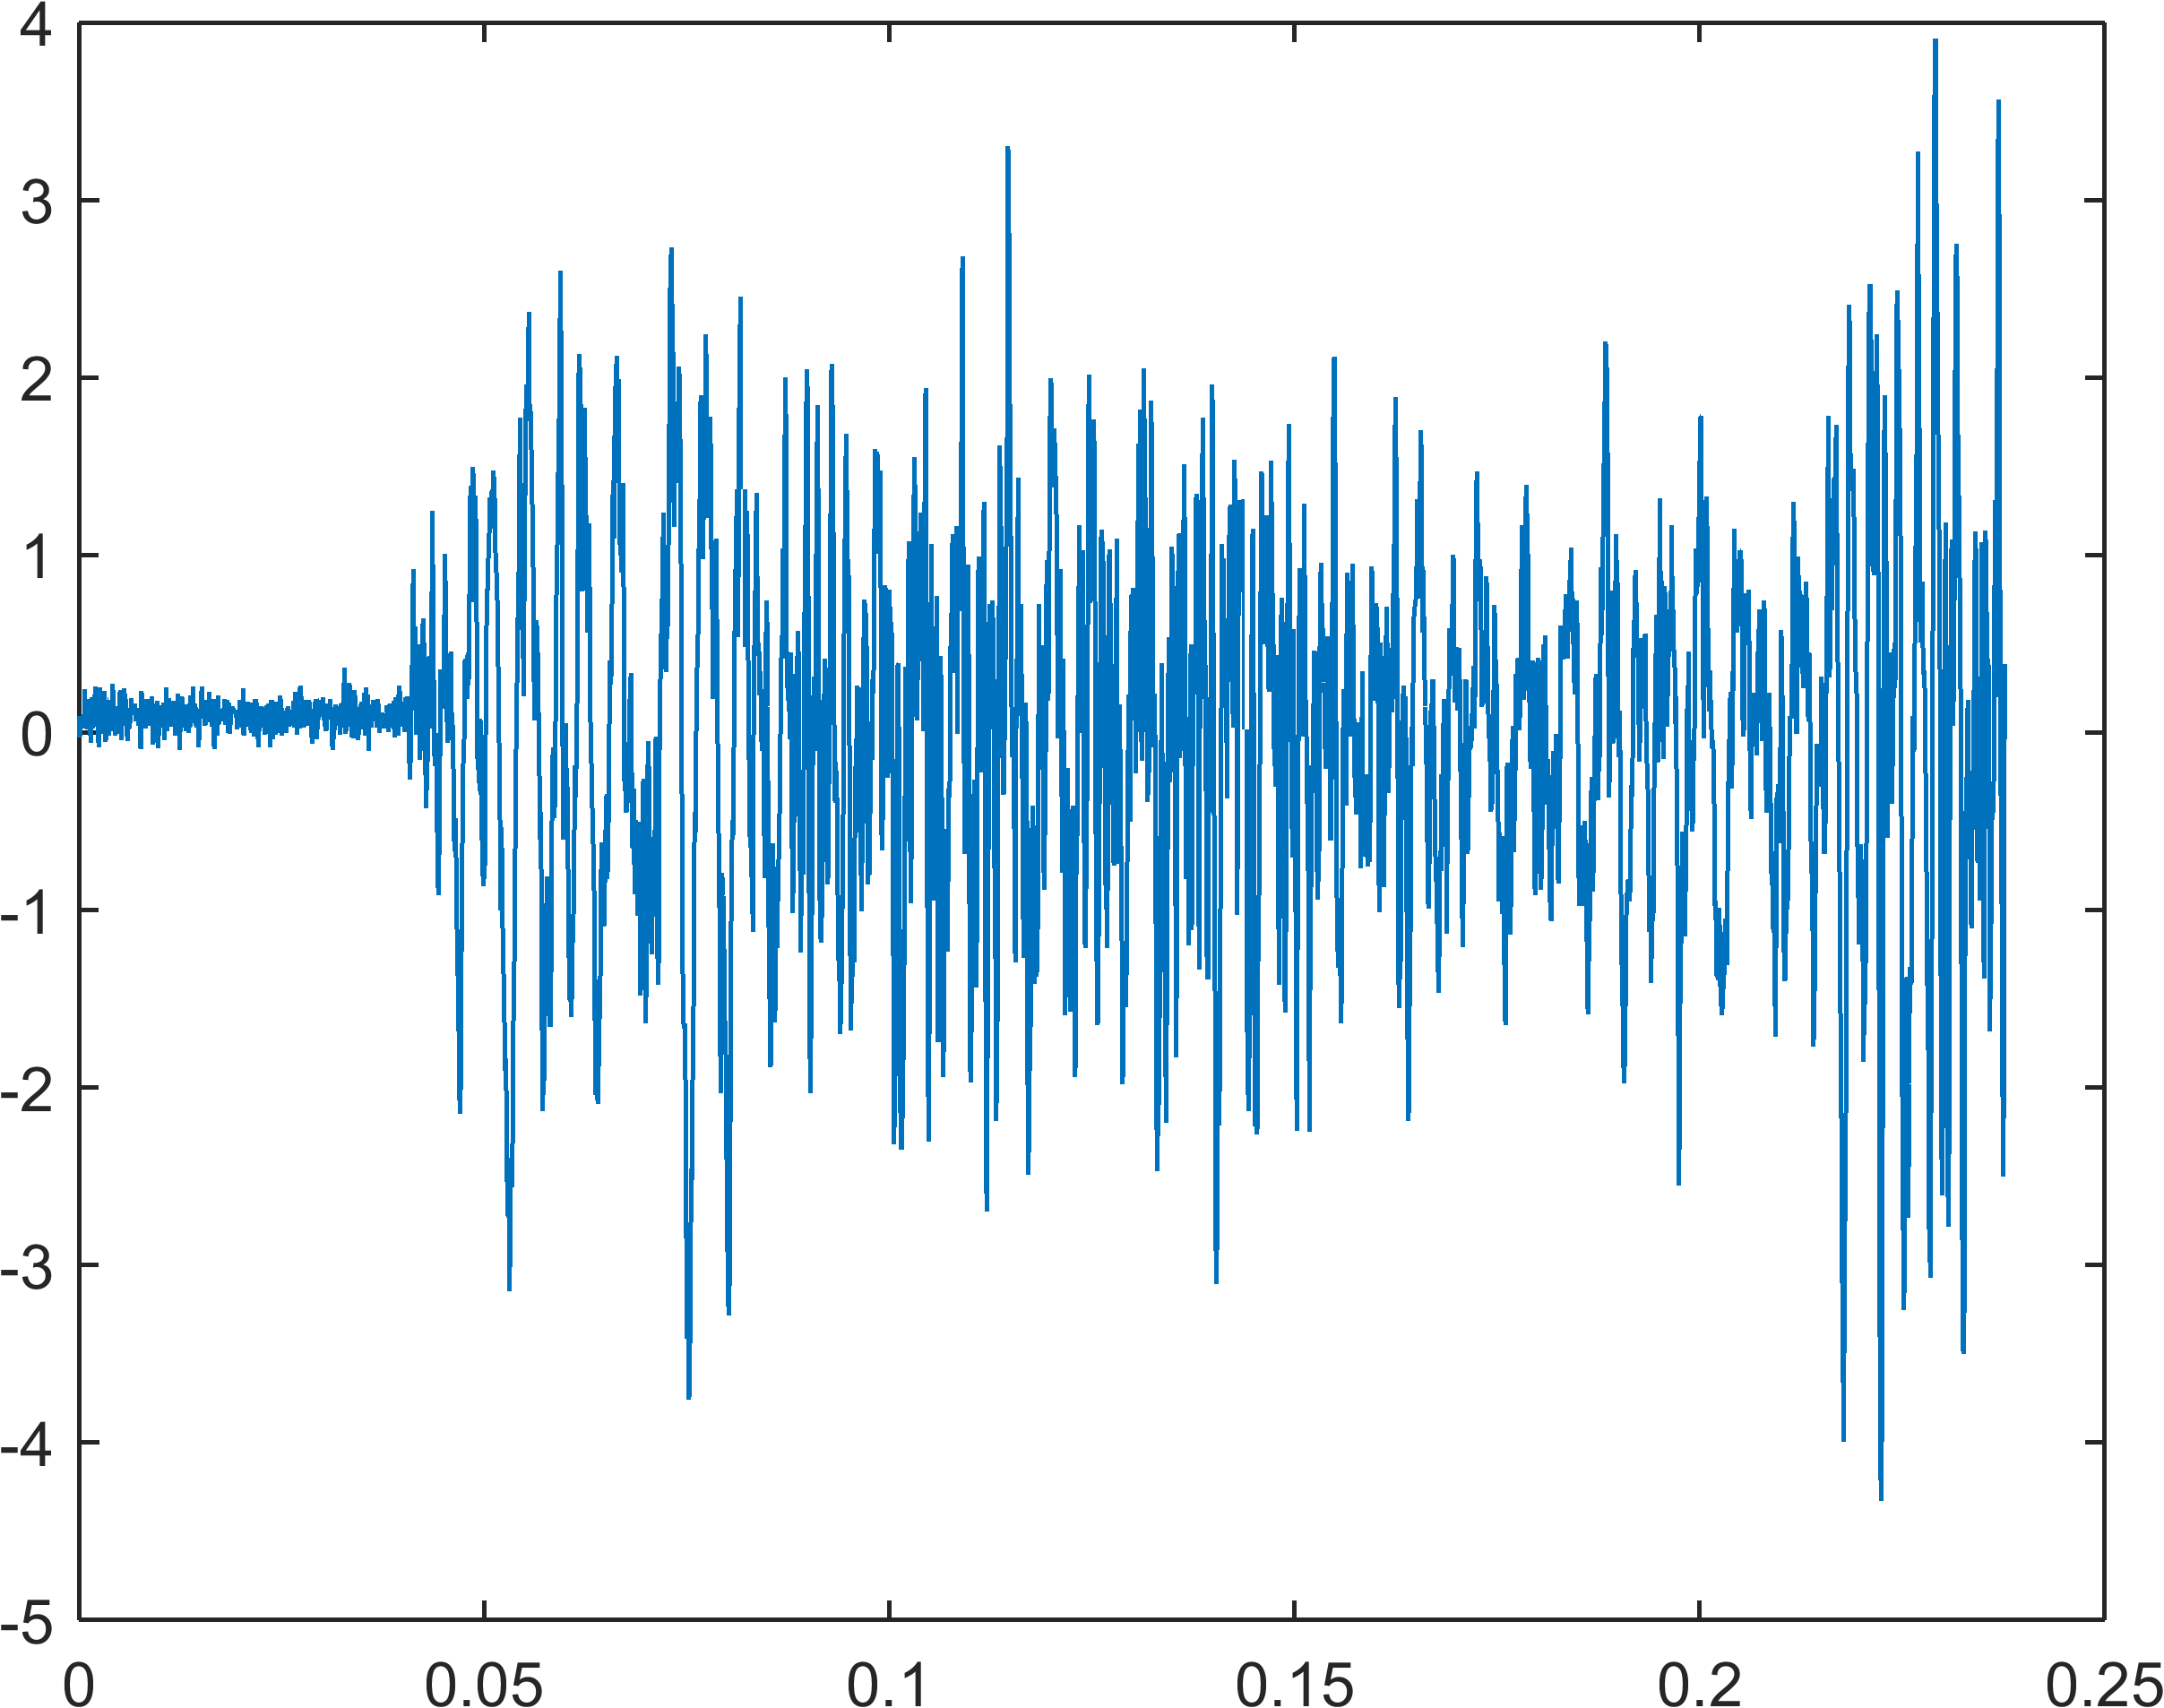
\includegraphics[width=0.3\textwidth]{imagesPart2/randomOutput}\label{subfig:randomOutput}}\quad
  \subfigure[Auto-correlation \(k(\tau)\) of the measured output fig: \ref{subfig:randomOutput}]
  {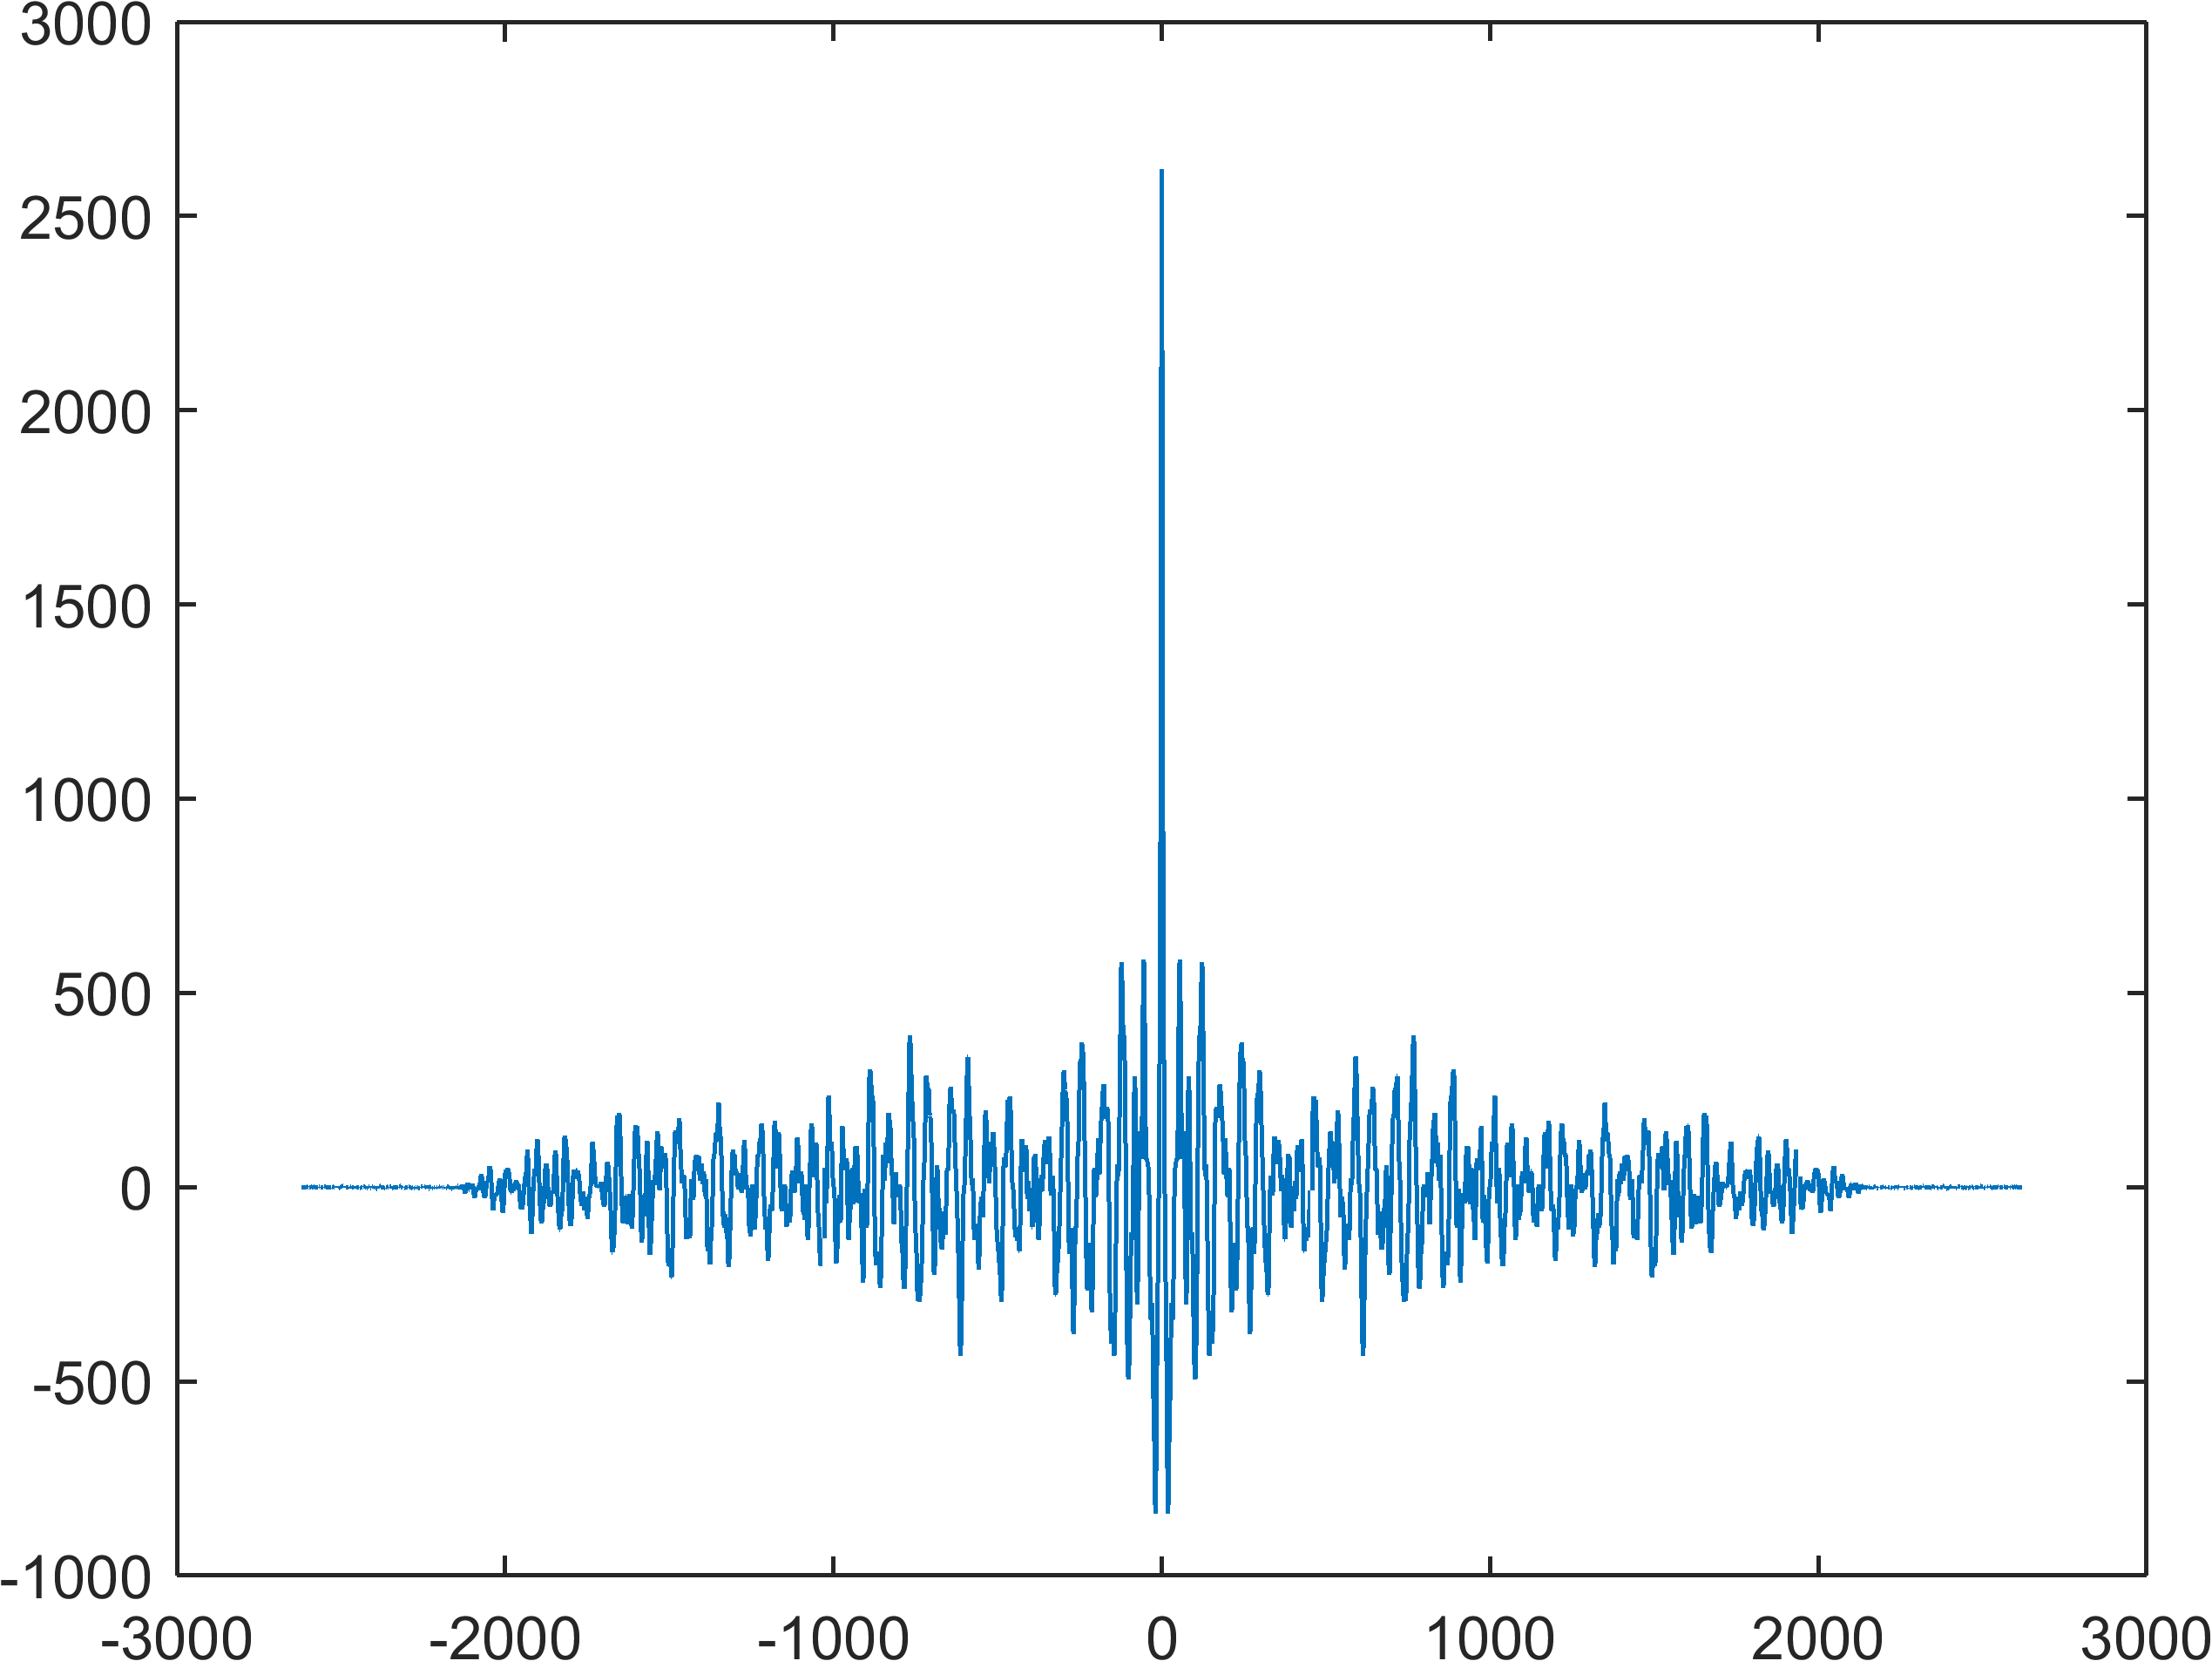
\includegraphics[width=0.3\textwidth]{imagesPart2/autocorrelationOutput}\label{subfig:autocorrelationOutput}}\quad
  \subfigure[Power spectrum density \(S(s)\) of the output fig: \ref{subfig:randomOutput}]
  {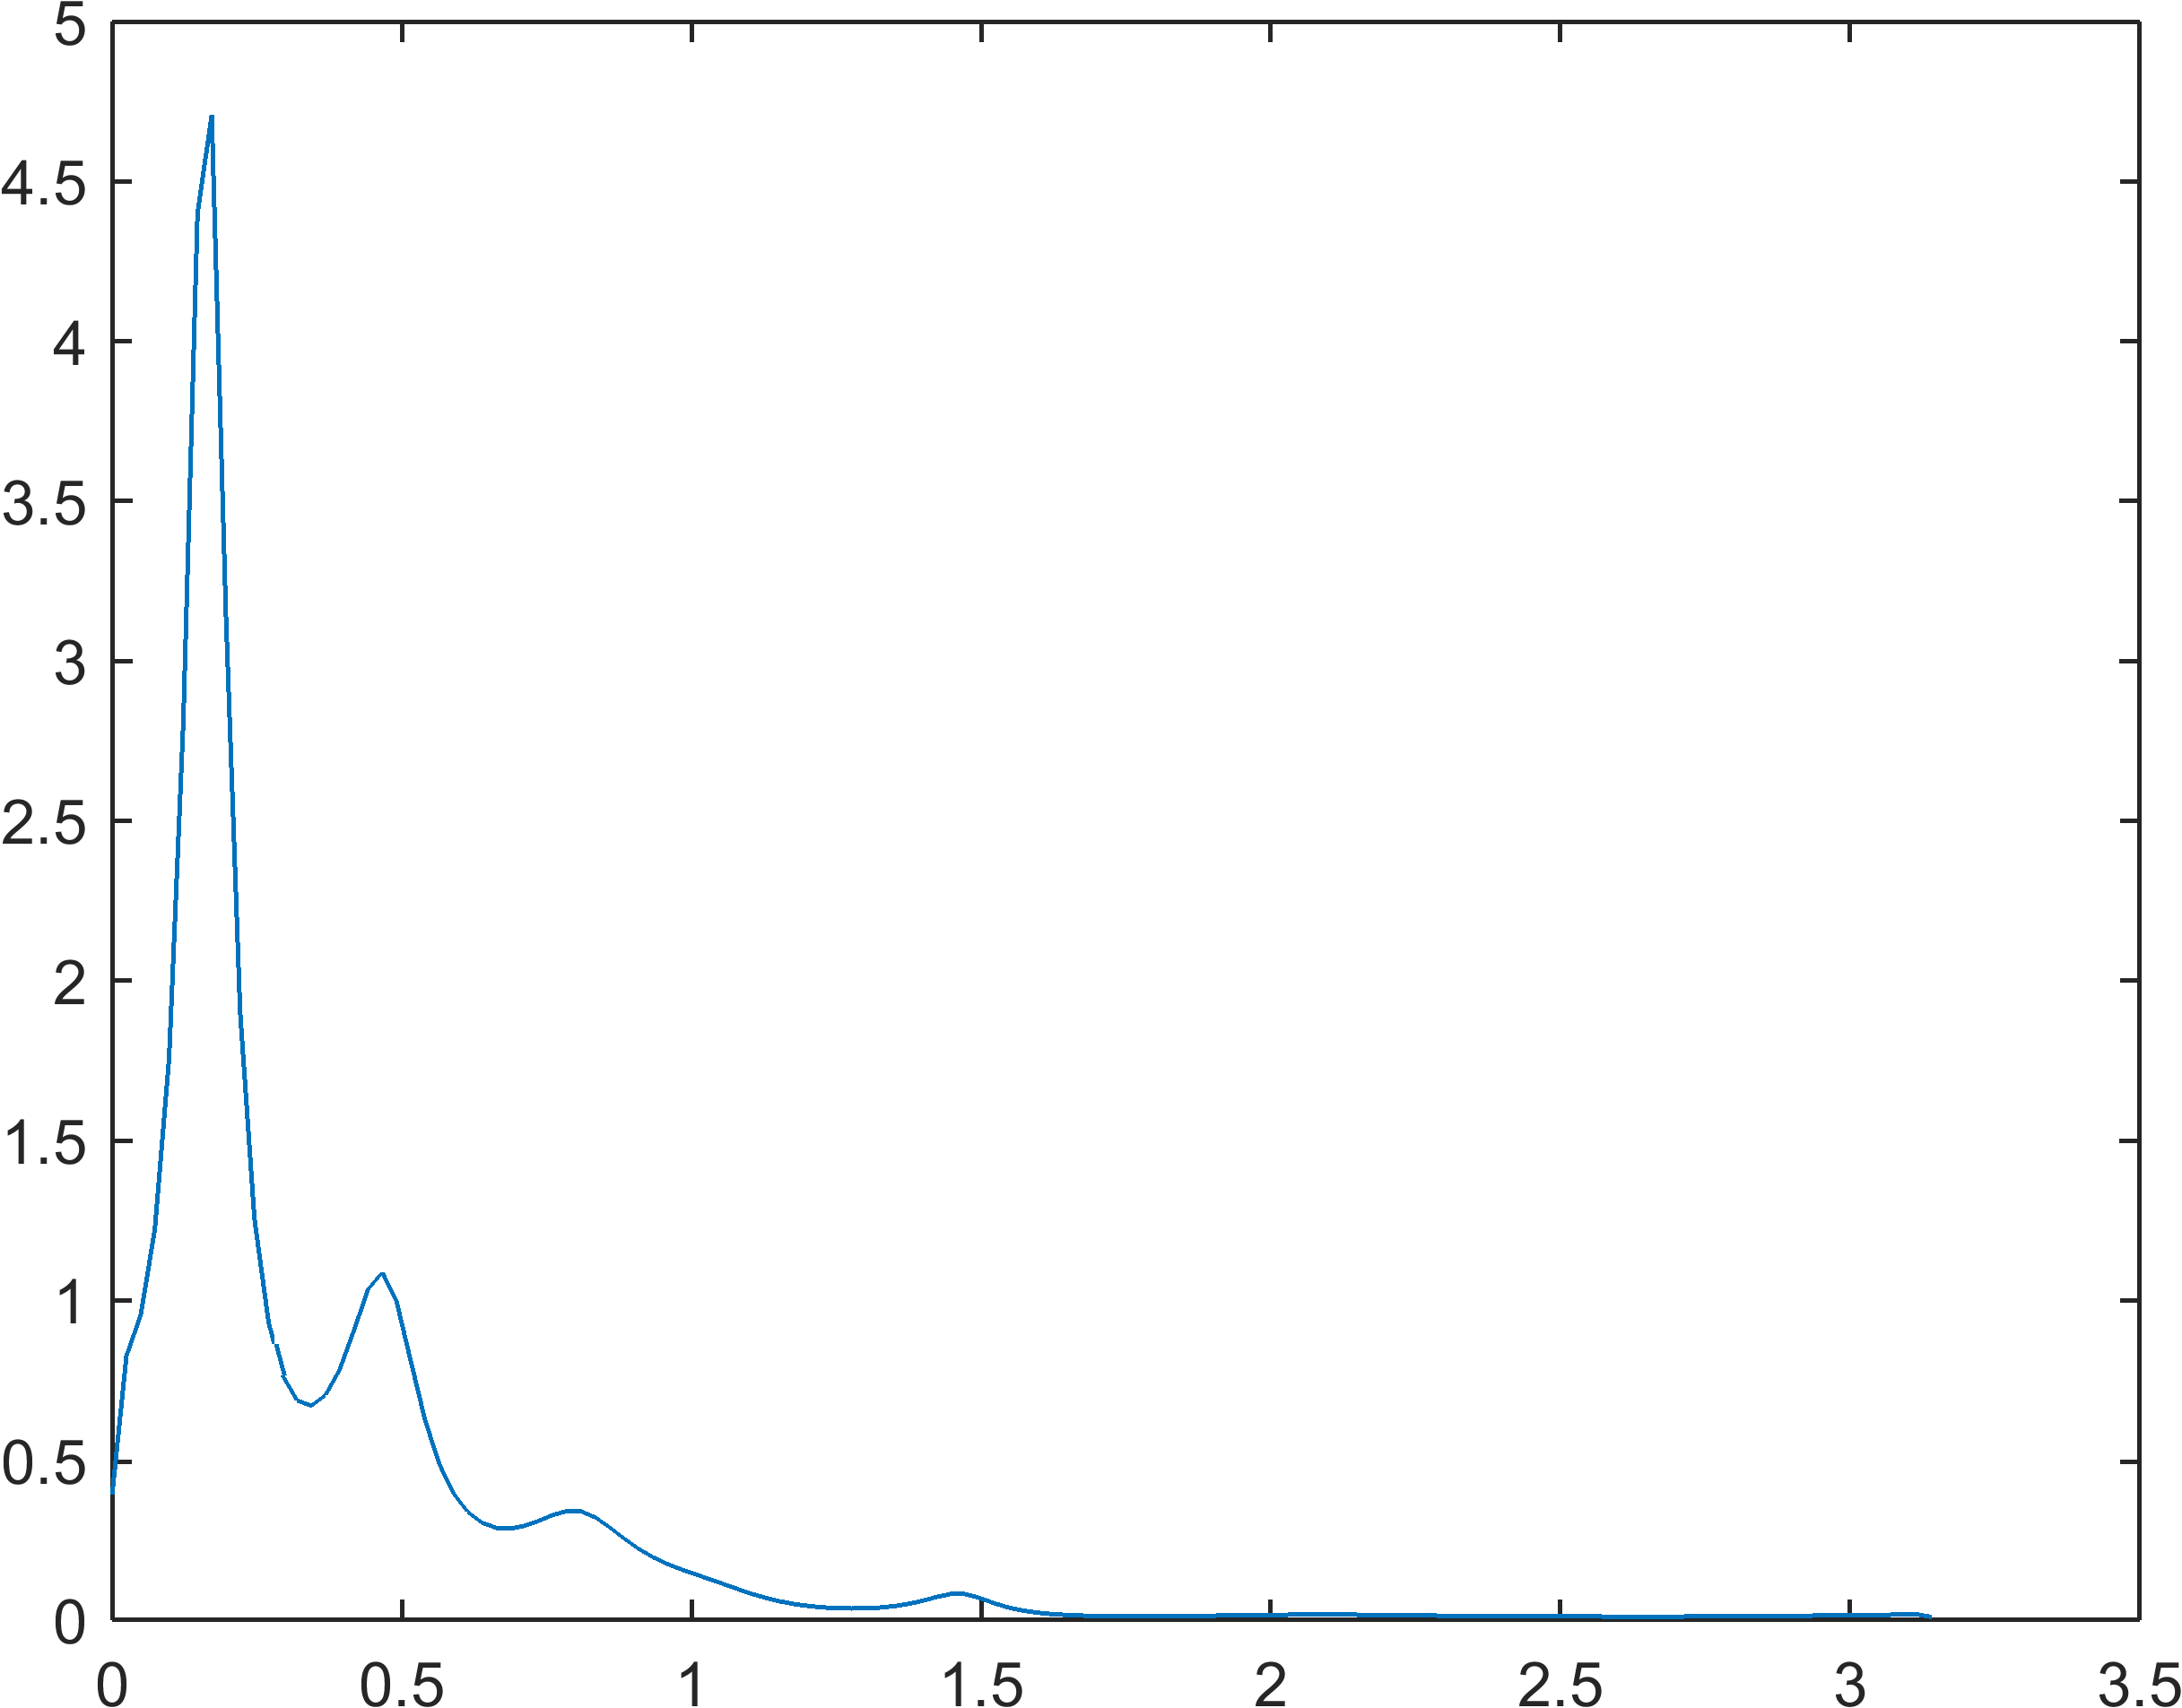
\includegraphics[width=0.3\textwidth]{imagesPart2/psdOutput}\label{subfig:psdOutput}}
  
  \caption{Different types of measurements for estimation of Modal parameters in OMA}
\end{figure*}

\renewcommand{\arraystretch}{1.2}
\begin{table}[!h]
    \centering
\begin{tabularx}{0.915\textwidth}{c|c|c}
  \hline
  Measurement & Auto-correlation & Power Spectrum \\
  \hline
  $x(t)$ & $k(\tau) = \int x(t)x(t-\tau)dt$ &  $S(s) = \int k(\tau)exp(-2 \pi i s^{T} \tau )d\tau$\\
  \hline \hline
  \multicolumn{3}{|c|}{Assumption: Second Order Differential}\\
  \hline
   & $ \sum A_{i}exp(-\lambda_{i}\tau)sin(B_{i}\tau)$ & $\frac{\sum a_{k}(s)^{k}}{\sum b_{l}(s)^{l}}$\\
   \hline \hline
   \multicolumn{3}{|c|}{Assumption: Gaussian Mixture Model}\\
   \hline
   $GP(0 , k_{SM})$ 
   & $  \sum w_{i} cos(2\pi\mu_{i}\tau) exp\{-2\pi^{2}\sigma_{i}^{2}\tau^{2}\}$ 
   & $ \sum w_{i}  \frac{1}{\sqrt{2\pi\sigma_{i}^{2}}}exp\{\frac{1}{2\sigma_{i}^{2}}(s-\mu_{i})^{2}\} $\\
   \hline
\end{tabularx}
\caption{Comparison of fitting functions}
  \label{tab:comparisonOfFittingFunctions}
\end{table}

While the modal parameters can be chosen by minimizing the least square error, how to choose the number of modes is a recurring question in several OMA algorithms. This problem is partially resolved by using stabilization diagrams or mode identification functions \cite{allemang1998unified, williams1985multivariate, shih1988complex}. But in practical situations engineering judgment is often required to estimate the optimal modal order. To automatically choose \(Q\), we use the Bayesian Information Criteria (BIC) \cite{findley1991counterexamples} which penalizes more complex models to estimate the parameter \(Q\). The BIC estimate has been earlier used to find the optimal functional form of covariance function \cite{duvenaud2013structure}

\textbf{\begin{equation}\label{eq:BIC}
    BIC(Q) = N\ln(ML) + N_{hyp}\ln(N)
\end{equation}}

Here, \(n\) denotes the number of data-points to fit, \(ML\) denotes the marginal likelihood of the fit and \(N_{hyp}\) denote the number of hyper-parameters to fit. The BIC performs a trade-off between the data-fit term \(N\ln(ML)\) and the complexity penalty term \(N_{hyp}\ln(N)\), basically penalizing for over-fitting. Lowest value of BIC is preferred. 

\textbf{Define an algorithm here on how to find the Q etc}

Generally, identification of modal frequencies requires engineering judgment, i.e. engineers have to look at the stabilization diagrams and figure out the optimal value of modal order. Using the Spectral mixture kernel we have encoded the knowledge of peaks in the power spectrum which in combination with BIC has eliminated the need to perform costly engineering judgment exercises and made the process automatic. We now compare the accuracy of finding modal frequencies using a spectral mixture kernel of NeXT methodology for a toy-dataset, and then later for a real dataset of HTC building \cite{brincker2000modal}.

\subsubsection{Results on a toy data-set}
In this section we conduct experiments, applying our approach on a highly damped 3 degree of freedom system\footnote{Dataset is available at github link: here}. As stated earlier we fit a GP model having zero mean and spectral mixture covariance on the measurements \(x(t)\) for varying number of Gaussian components \(Q\). We then evaluate the Bayesian Information Criteria to find the optimal value of \(Q\) for this measurement. The results of automatic identification are then compared to that of NeXT identification method. 

All experiments were performed on an Intel quad-core processor with 4Gb RAM. The Spectral Mixture technique suffers from multiple minimas and thus care should be taken while initializing the hyper-parameters\footnote{We first fit a Gaussian Mixture model on the power spectrum to initialize the hyper-parameters and then optimize the marginal likelihood for speedy optimization.}.  

Table \ref{tabComparisonOfModalFrequenciesToyData} shows the comparison of frequencies for Modal frequencies predicted using NeXT algorithm and Spectral Mixture algorithm. We can observe that the NeXT method cannot predict the third frequency with enough accuracy. 

\renewcommand{\arraystretch}{1}
\begin{table}[!h]
    \centering
\begin{tabular}{|l|l|l|l|}
  \hline
   & Real Frequency & NeXT Frequency & Spectral Mixture\\
  \hline 
  \hline
First Frequency (Hz) & 17.5 & 17.88 & 17.55\\
Second Frequency (Hz)  & 30 & 28.97 & 28.75\\
Third Frequency (Hz) & 35 & 39.32 & 36.80\\
   \hline
\end{tabular}
\caption{Comparison of Modal frequencies for toy data-set}
  \label{tabComparisonOfModalFrequenciesToyData}
\end{table}

Figure \ref{subfig:stabilizationDiagram} shows the stabilization diagram with increasing number of gaussians $Q$. The number of modal frequencies is dependent on the number of Gaussian components (\(Q\)), since each component will have only one mean value. As we progressively increase the number of components we start getting more and more modal frequencies. We call a frequency as stabilized if the difference between modal frequencies of two subsequent \(Q\) is less than \(1\%\), the green points are stabilized frequencies. The, figure \ref{subfig:bicVsQ} shows the BIC criterion with increasing number of Gaussian's $Q$. We can see that that the BIC is minimum for $Q=6$ and hence if we add anymore Gaussians for our dataset we will be over-fitting. The red line in figure \ref{subfig:stabilizationDiagram} shows the modal frequency with minimum BIC and hence the results of prediction.

\begin{figure*}[!ht]
  \centering
  \subfigure[Stabilization diagram with increasing number of gaussians $Q$, the dots denote the stabilized frequencies. We can observe that as the number of $Q$ increases the algorithm starts finding better and better modes.]
  {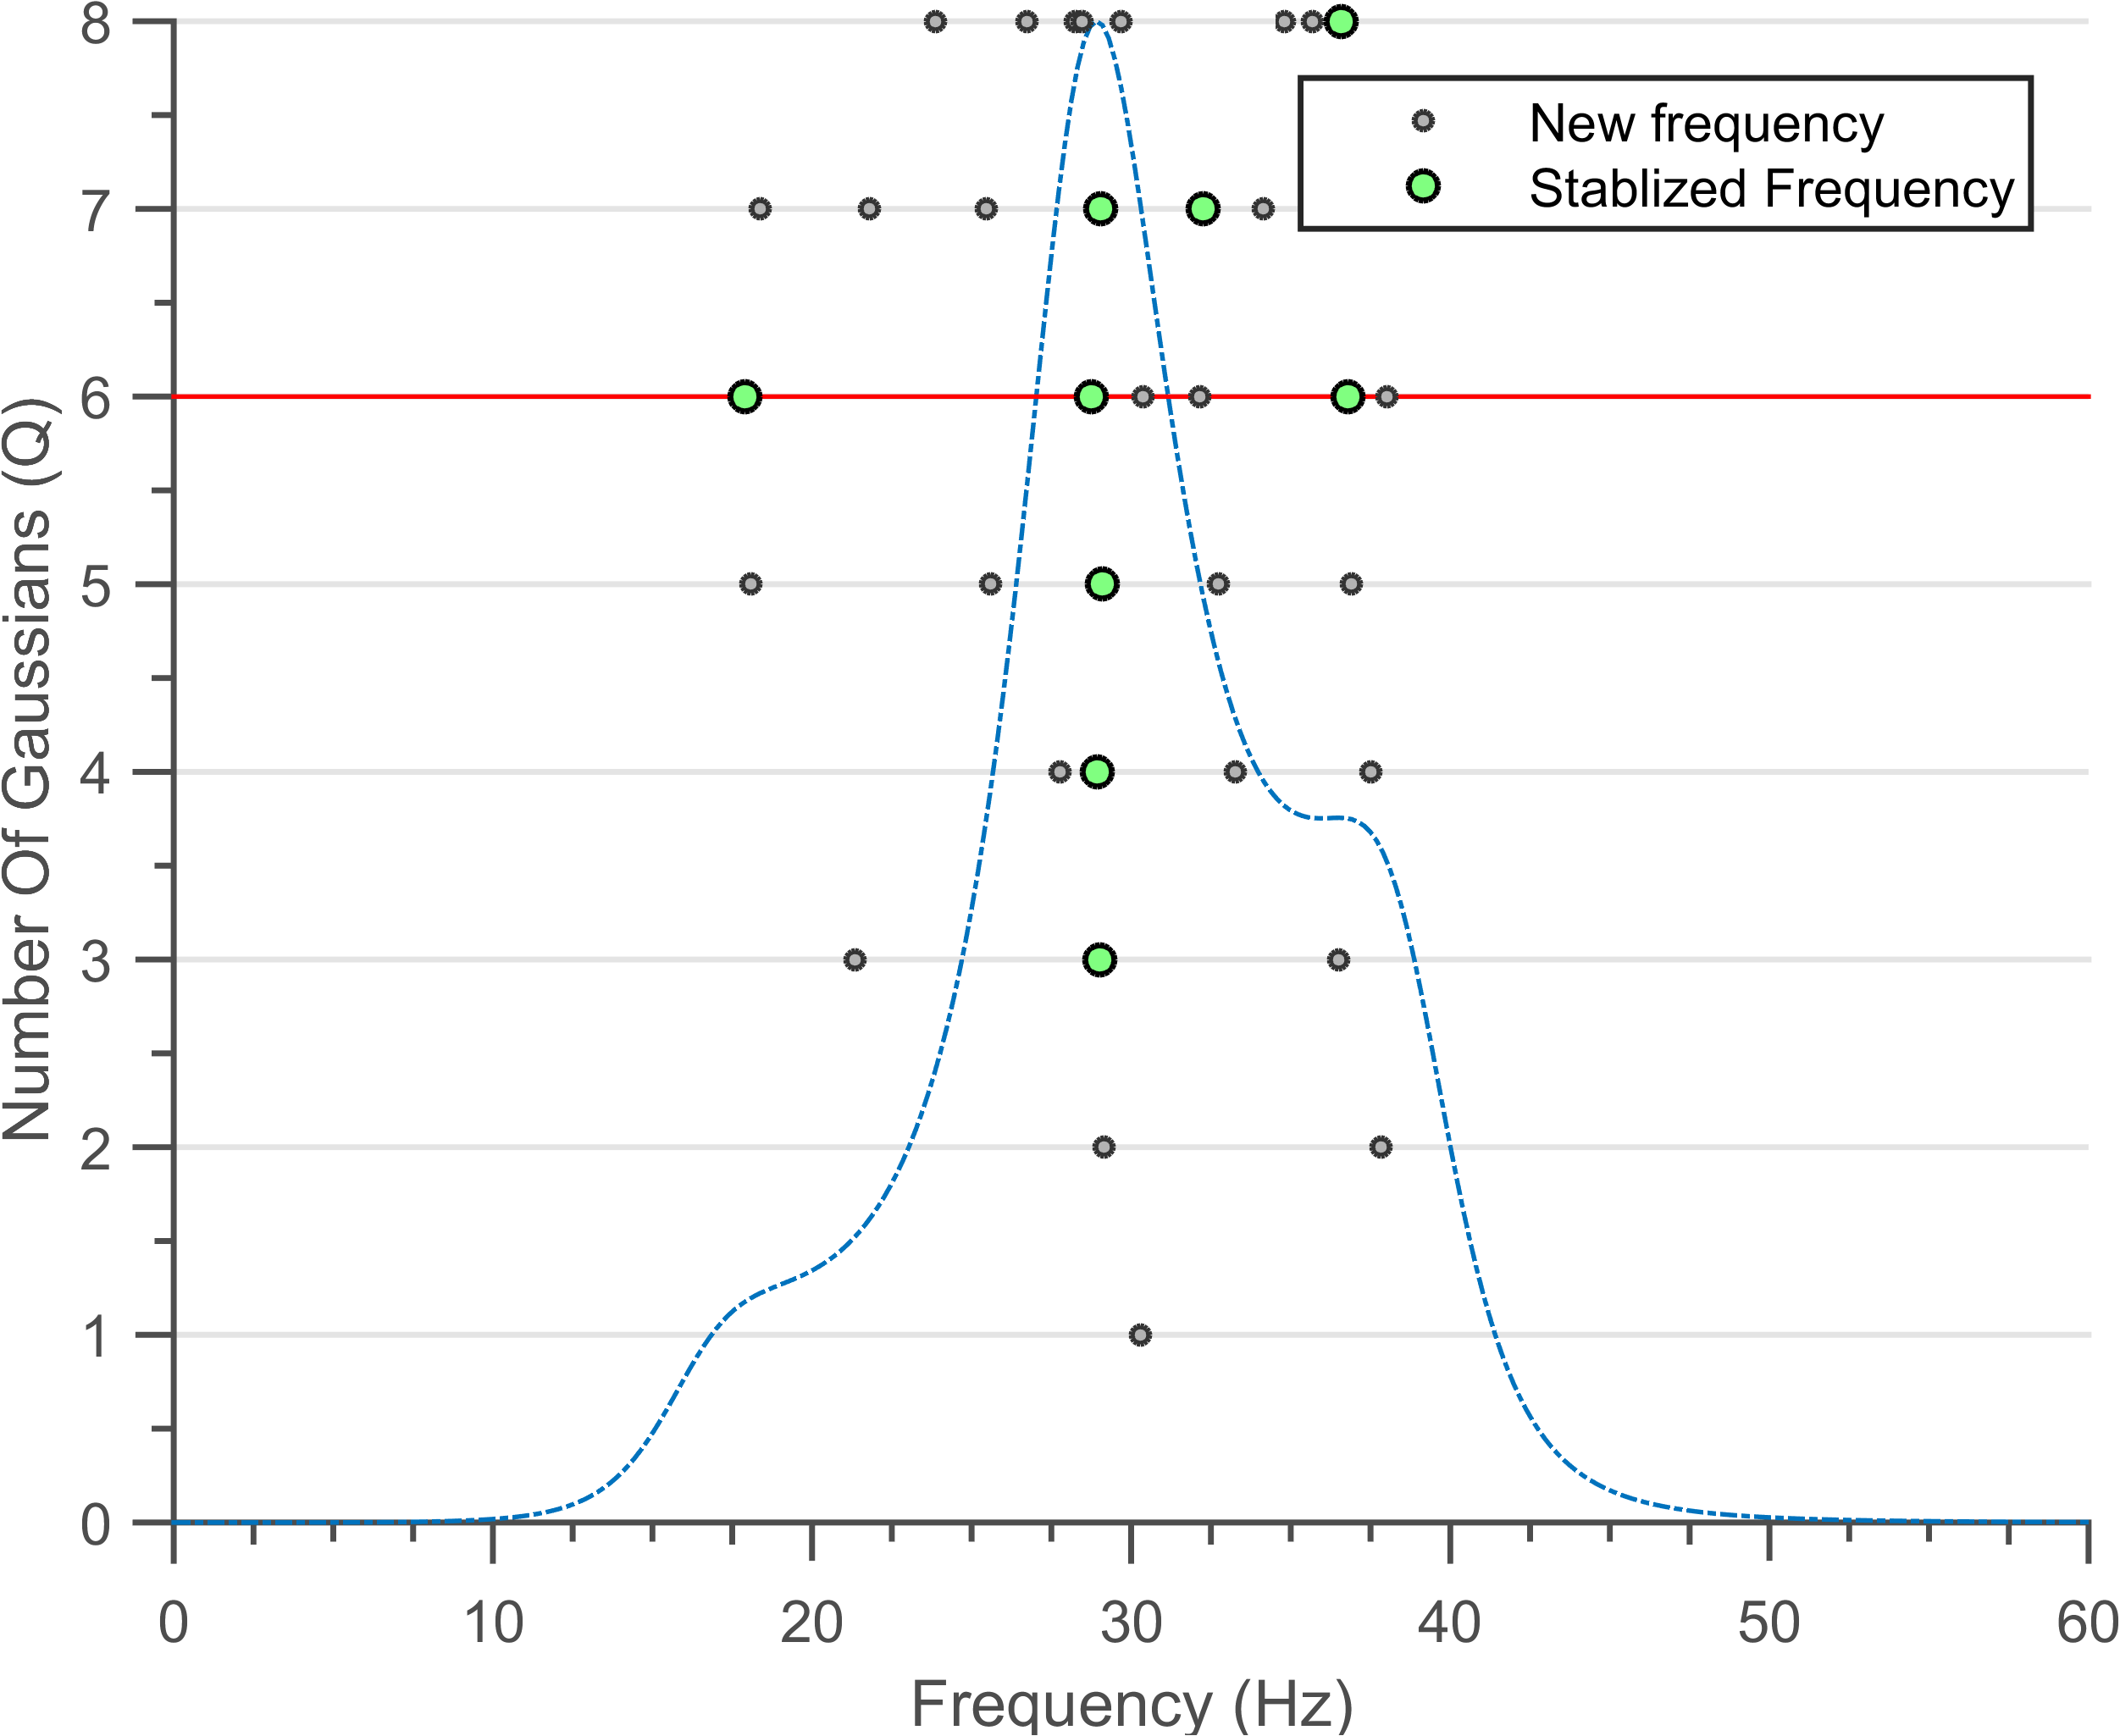
\includegraphics[width=0.45\textwidth]{imagesPart2/stabilizationDiagram_toyData}\label{subfig:stabilizationDiagram}}\quad
    \subfigure[The BIC criterion with increasing number of gaussian's $Q$. We can see that that the BIC is minimum for $Q=6$ and hence if we add anymore gaussian's for our dataset we will be performing over-fitting]
  {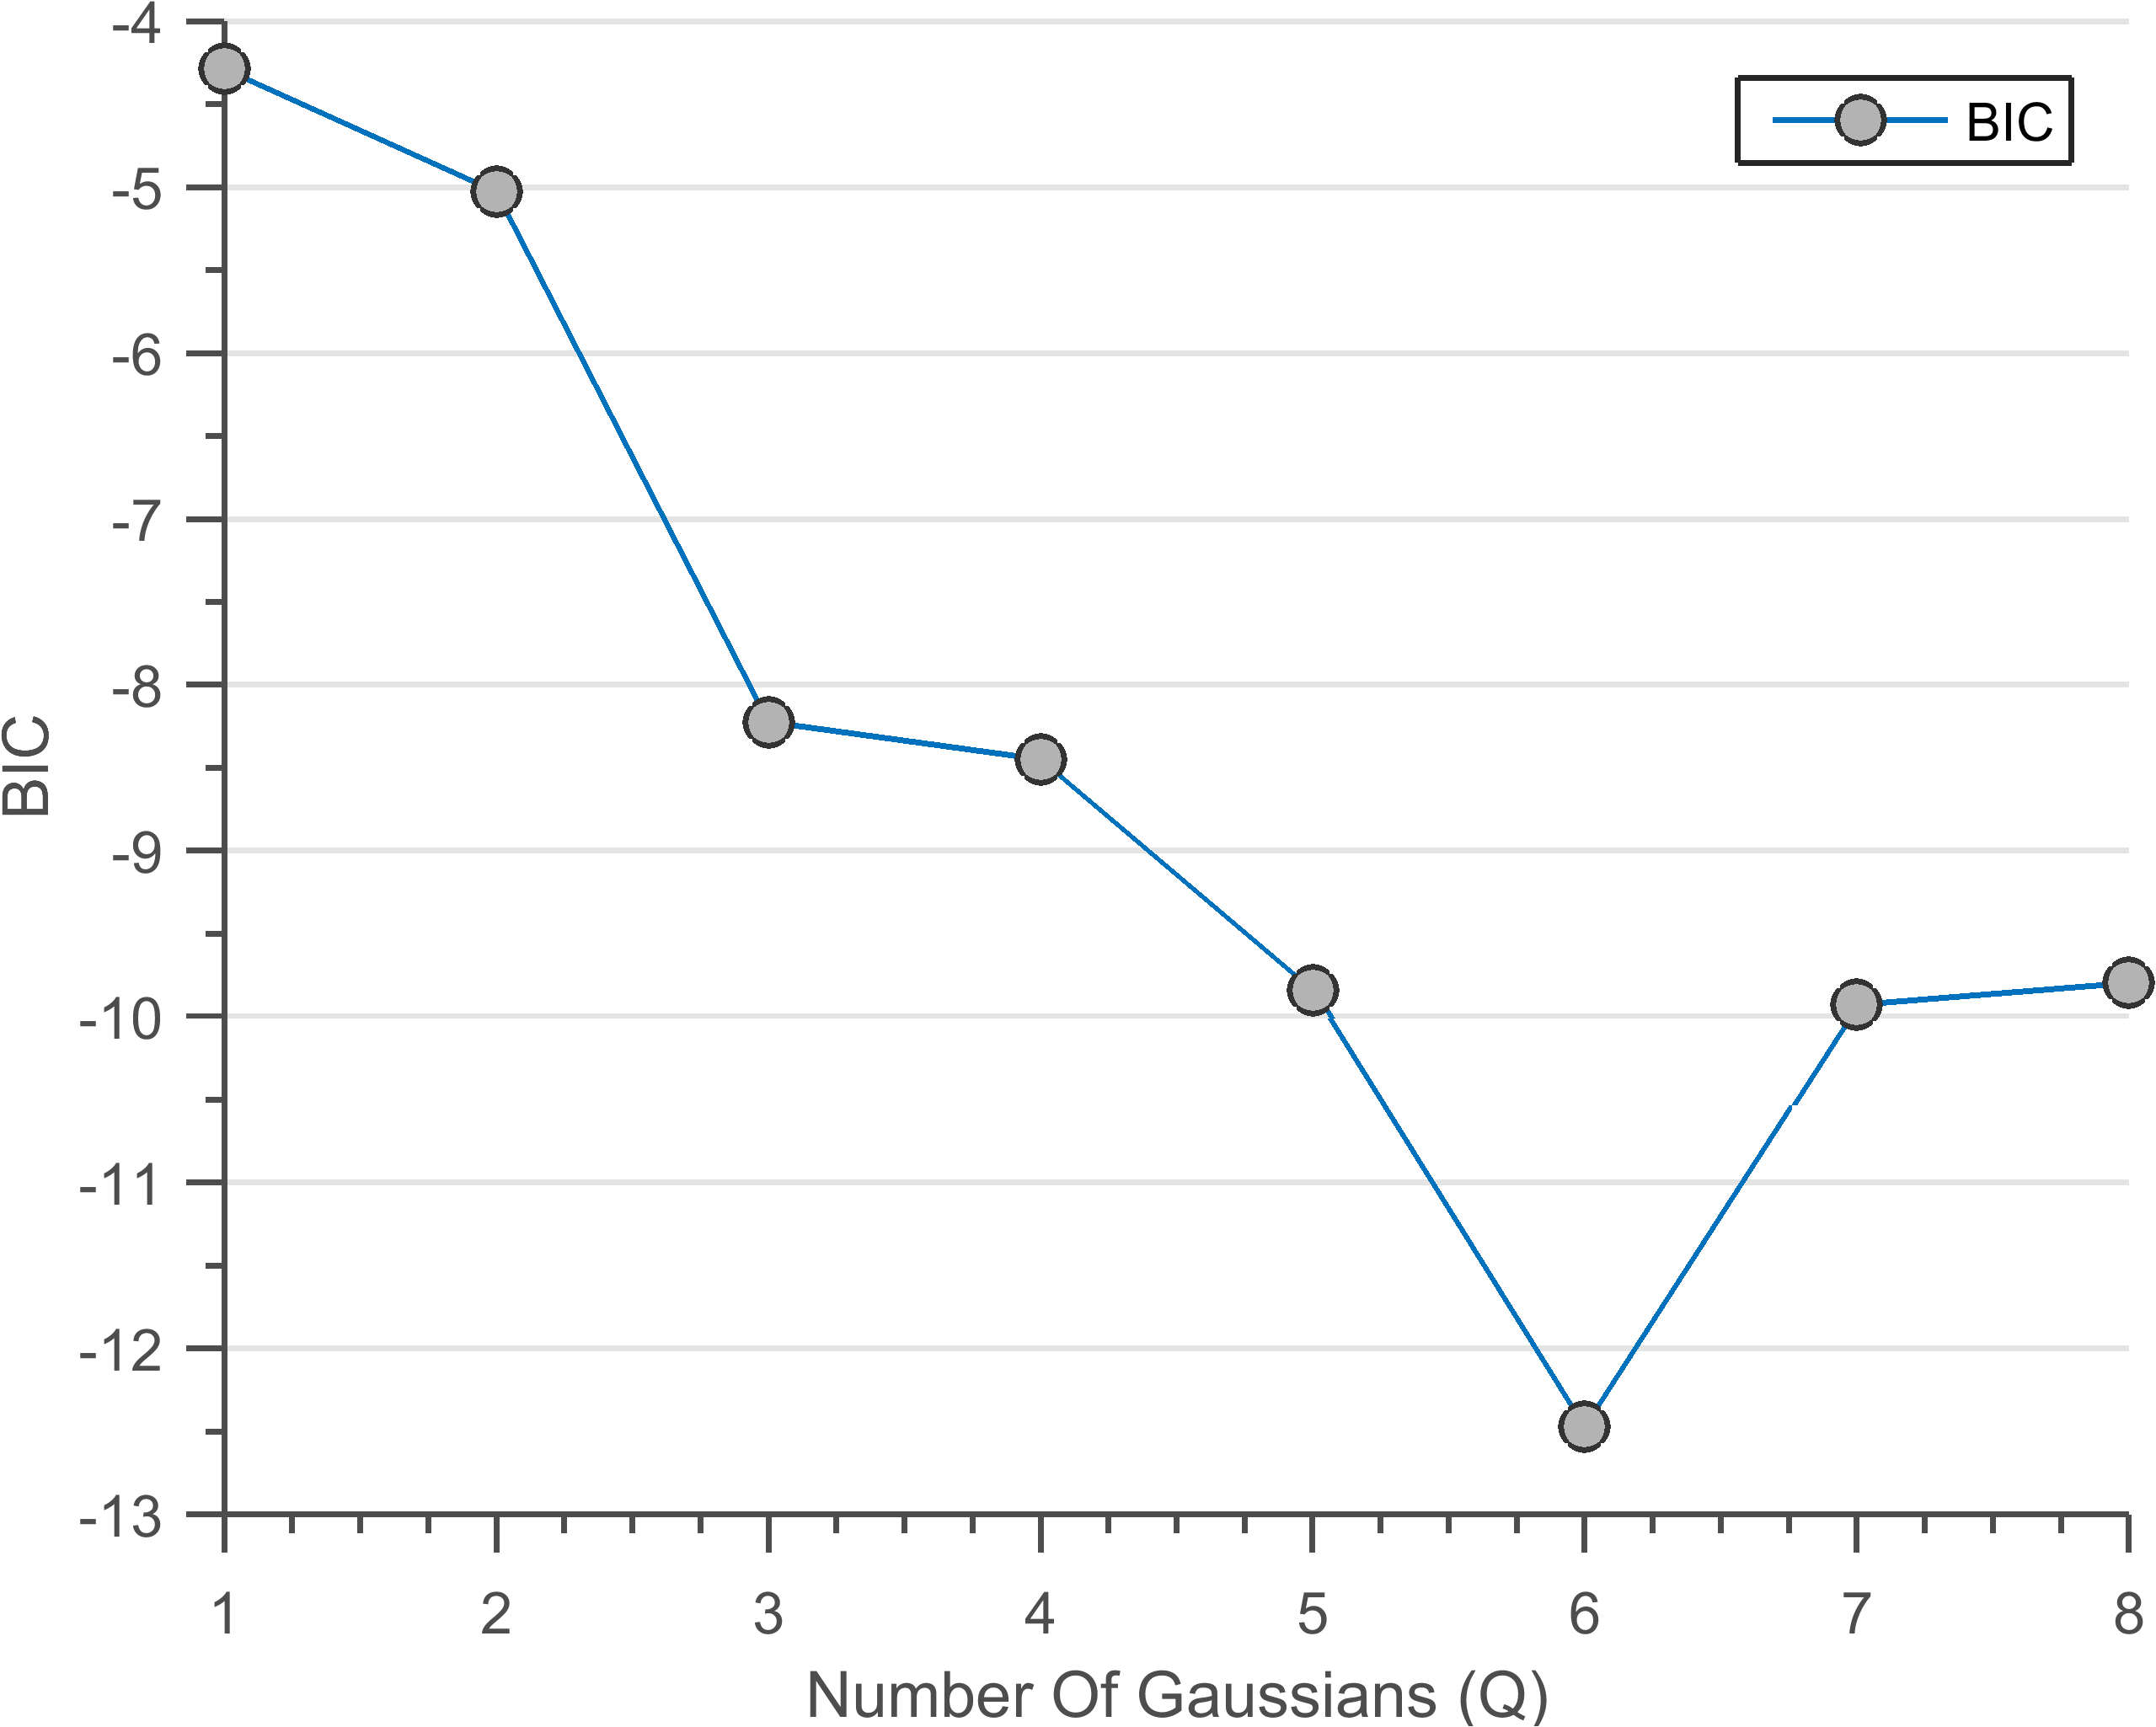
\includegraphics[width=0.45\textwidth]{imagesPart2/bicVsQ}\label{subfig:bicVsQ}}\quad
  
  \caption{Results of spectral mixture kernels on a toy dataset}
\end{figure*}

\subsubsection{Results on a HTC building dataset}
We now compare the predictions of the models on an ambient response of Heritage Court Building\footnote{The data is available at : http://www.brinckerdynamics.com/oma-toolbox}. The responses are measured at 6 different points on the building resulting in 6 different power spectrums. 

We compare the modal frequencies obtained using Spectral Mixture kernel with the modal frequencies obtained in the original paper \cite{brincker2000modal}. To compare the performance we automatically identify modal frequencies present in each of the 6 power spectrums and take the mean of the stabilized frequencies.

Table \ref{tabComparisonOfModalFrequenciesToyData} shows the comparison of Modal frequencies predicted in \cite{brincker2000modal} with Spectral Mixture algorithm. The results of the two methods are very similar, although the frequencies obtained by spectral mixture GP are completely automatic. 

\renewcommand{\arraystretch}{1}
\begin{table}[!h]
    \centering
\begin{tabular}{|l|l|l|}
  \hline
    & Spectral Mixture & \cite{brincker2000modal} \\
  \hline 
  \hline
First Frequency (Hz) & 1.23 & 1.23\\
Second Frequency (Hz)  & 1.29 & 1.27\\
Third Frequency (Hz) & 1.43 & 1.45\\
Fourth Frequency (Hz) & 3.87 & 3.86\\
Fifth Frequency (Hz) & 4.28 & 4.25\\
   \hline
\end{tabular}
\caption{Comparison of Modal frequencies for HTC data-set}
  \label{tabComparisonOfModalFrequenciesHTCData}
\end{table}

\begin{figure*}[!ht]
  \centering
  \subfigure[Stabilization diagram for one of the 6 power spectrums. The green dots denote the stabilized frequencies, the red line is denotes minimum BIC. We can observe that as the number of $Q$ increases the algorithm starts finding better and better modes.]
  {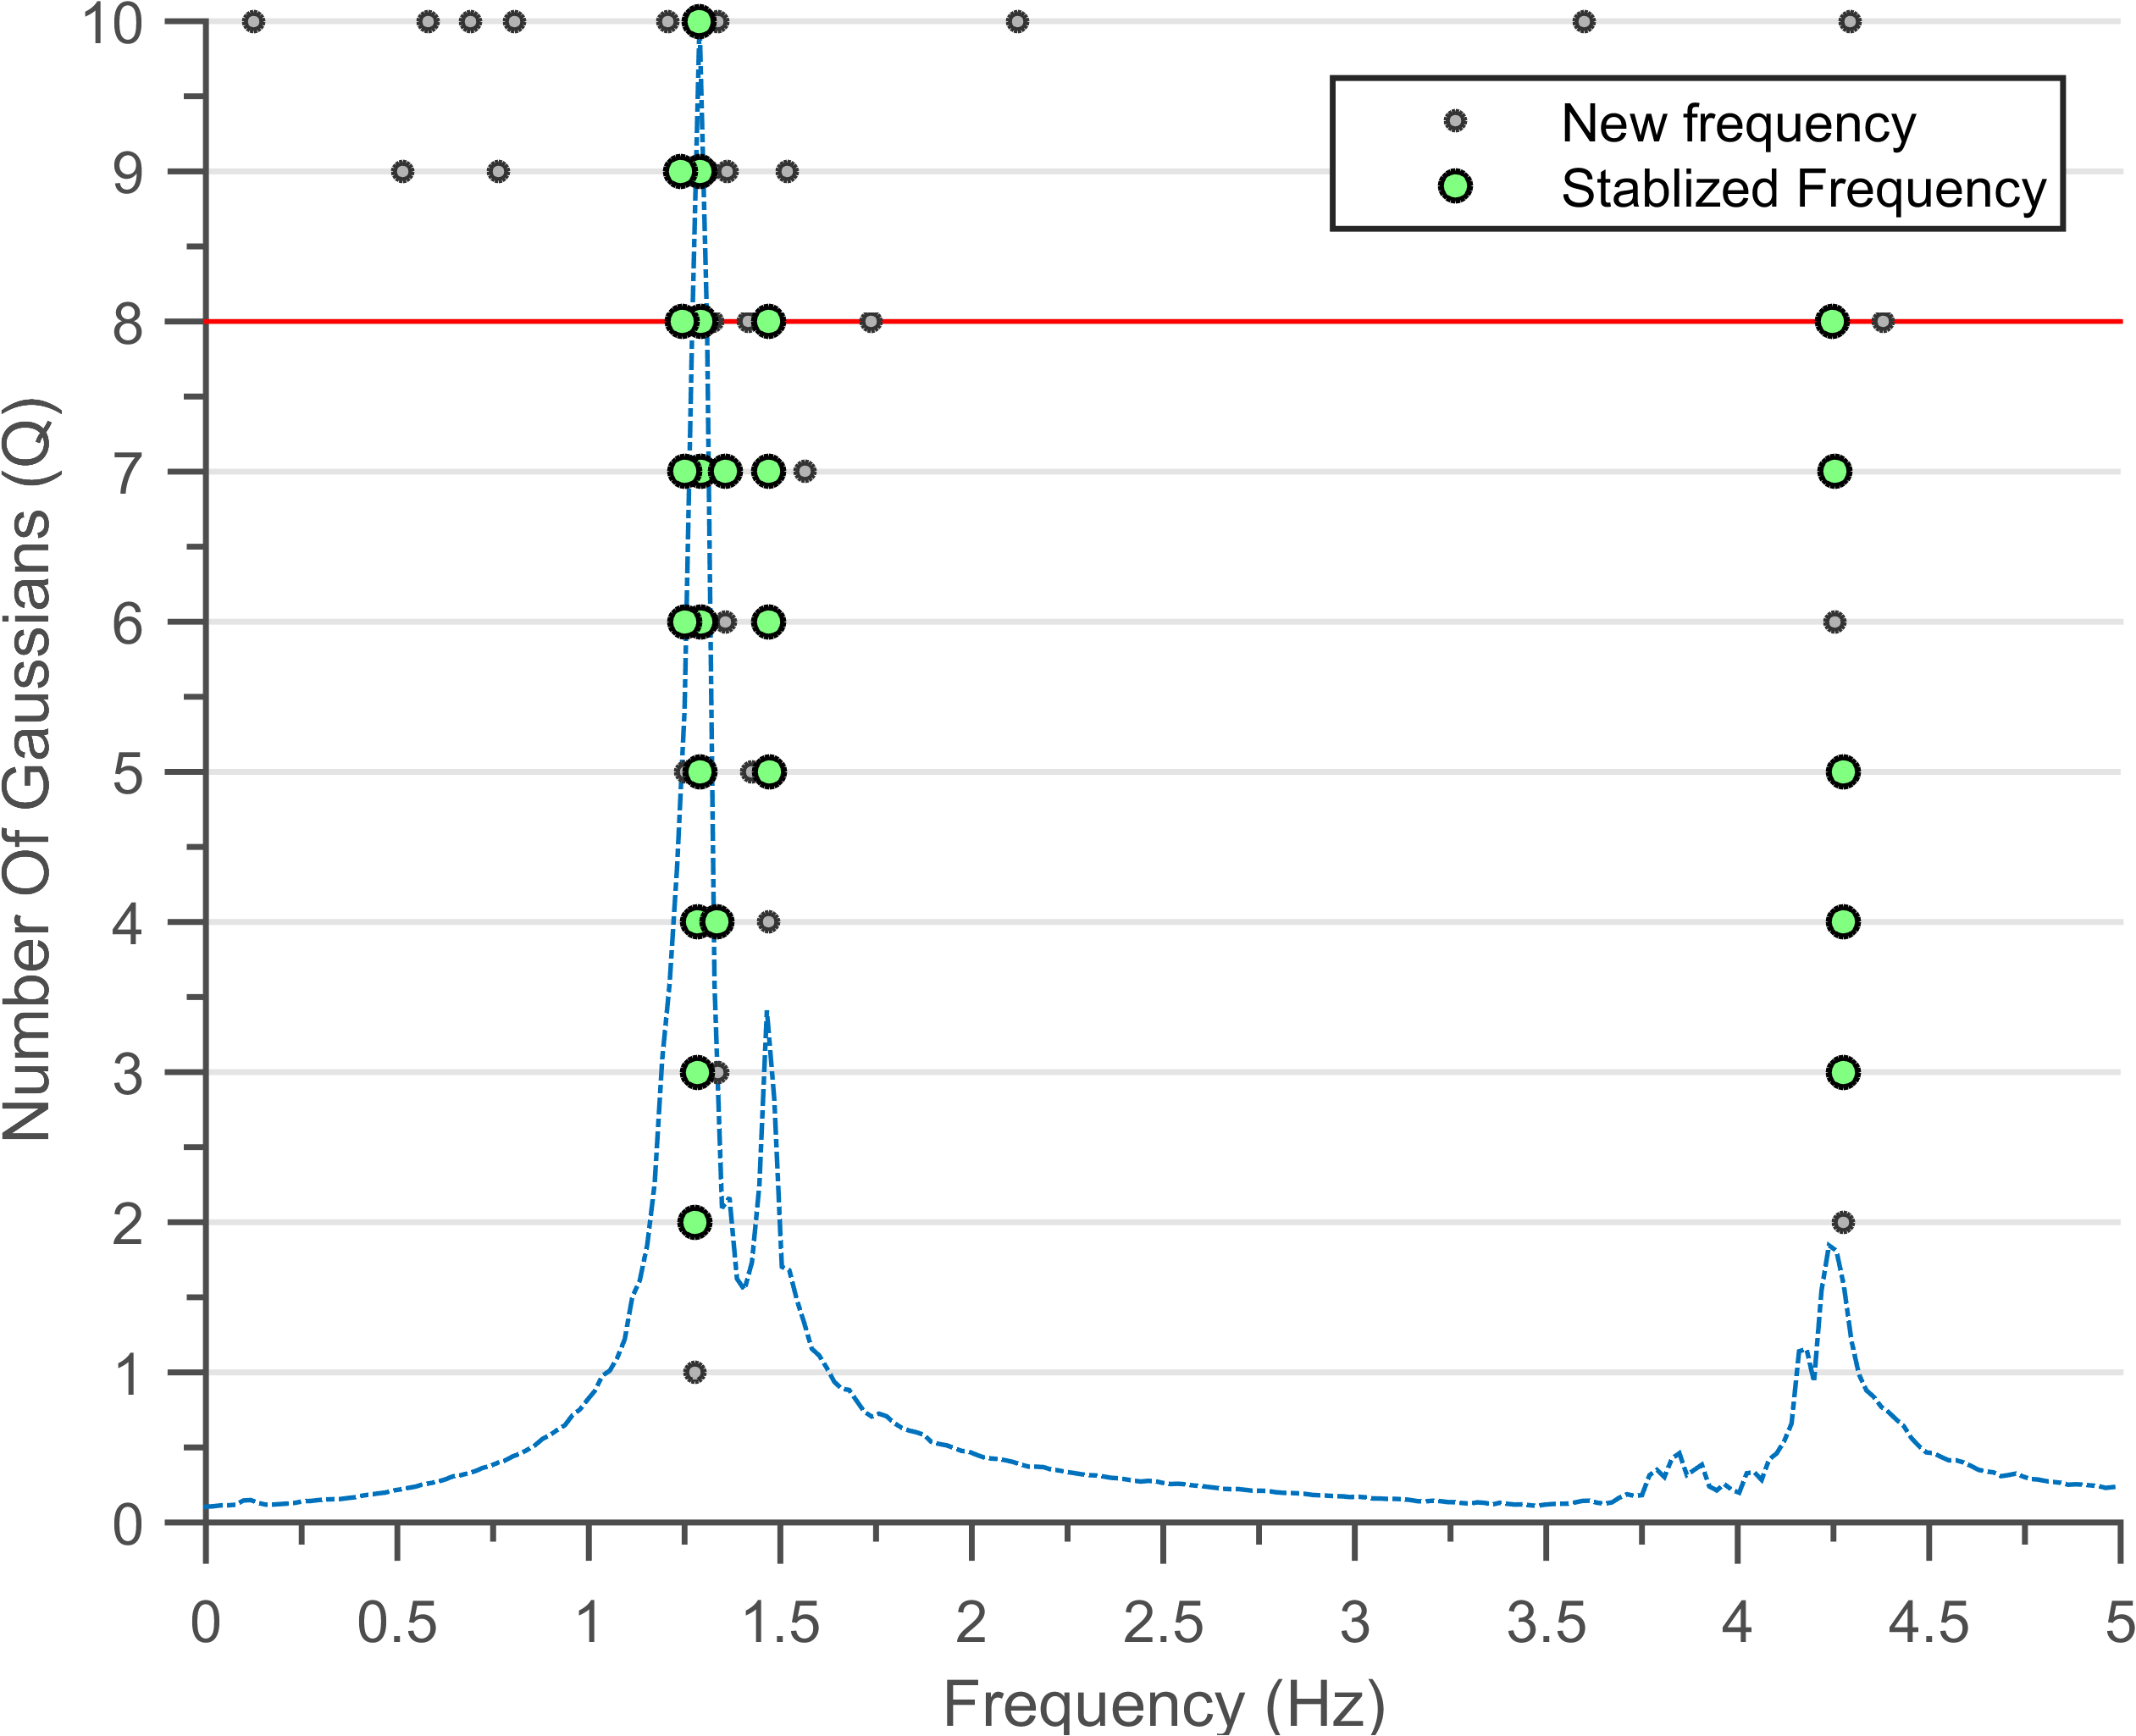
\includegraphics[width=0.45\textwidth]{imagesPart2/stabilizationDiagram_HTCBuildingData}\label{subfigStablizationHTCData}}\quad
    \subfigure[The BIC criterion with increasing number of gaussian's $Q$. We can see that that the BIC is minimum for $Q=8$ and hence if we add anymore gaussian's for our dataset we will be performing over-fitting]
  {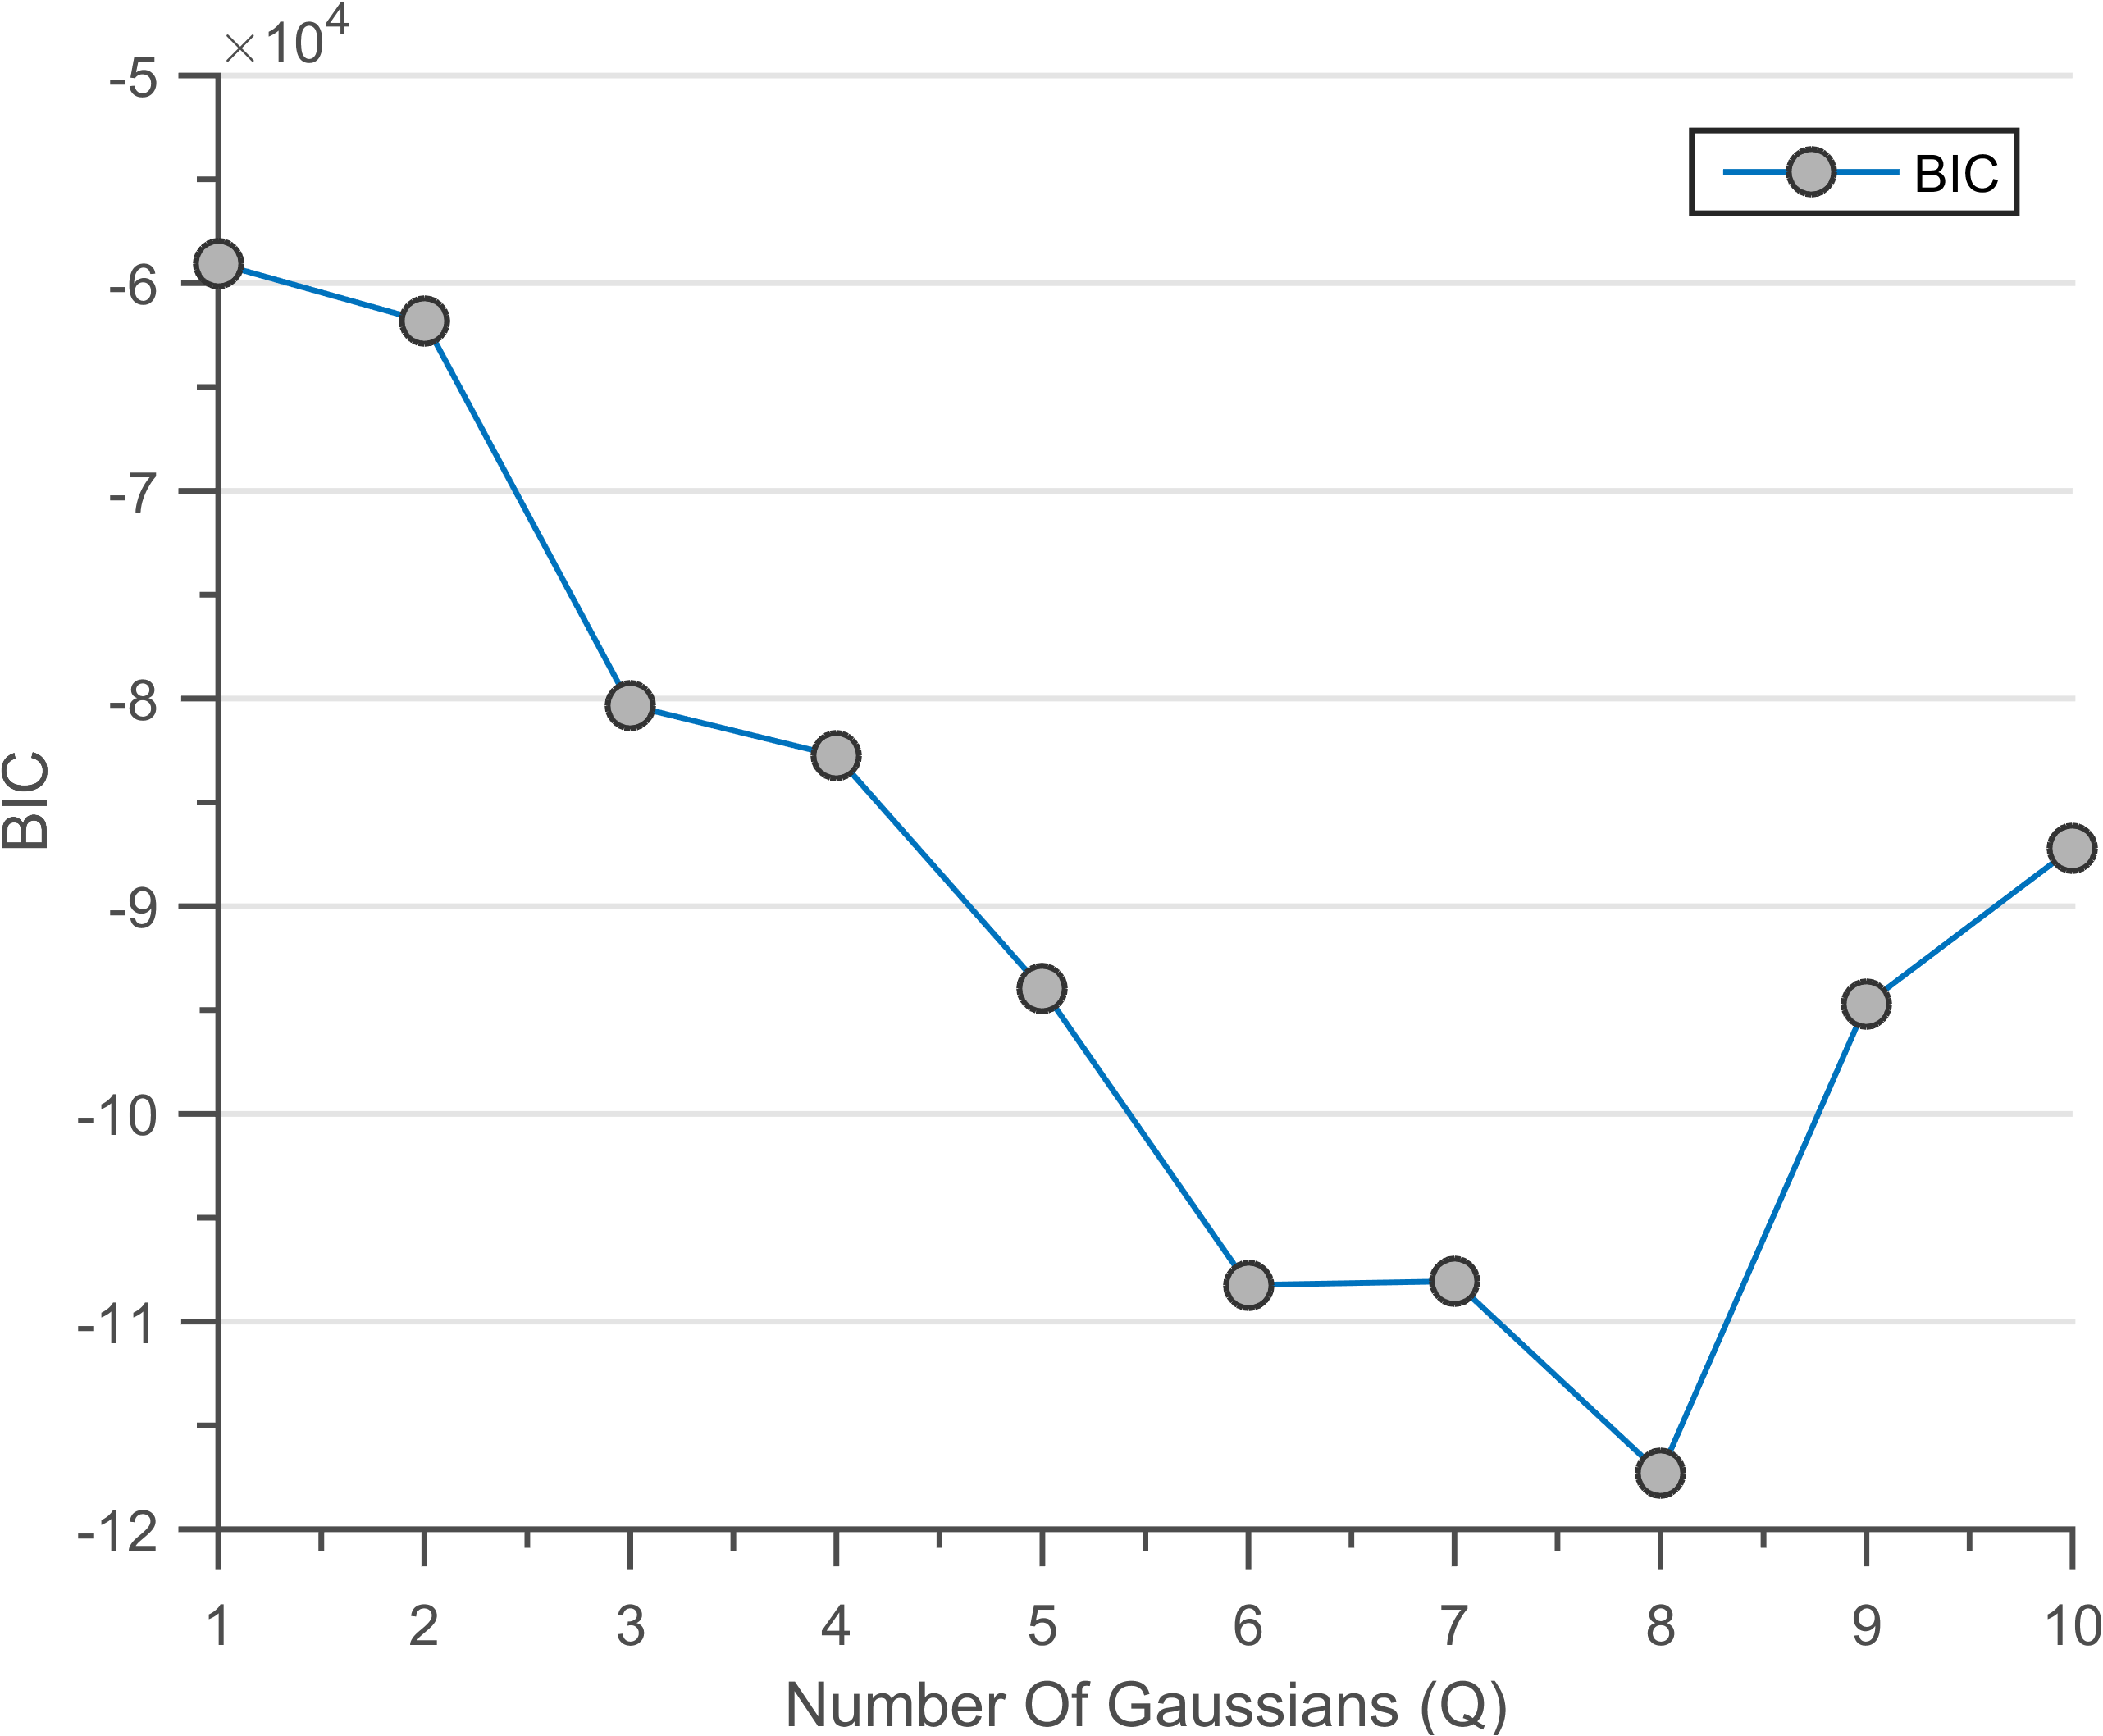
\includegraphics[width=0.45\textwidth]{imagesPart2/bicVsQ_HTCBuilding}\label{subfigBICHTC}}\quad
  
  \caption{Results of spectral mixture kernels on real data from HTC building}
\end{figure*}

Figure \ref{subfigStablizationHTCData} shows the stabilization diagram with increasing number of gaussians $Q$. We can observe that as the number of $Q$ increases the algorithm starts finding better and better modes. We can observe that there are three modes which start stabilizing from $Q=5$. The, figure \ref{subfigBICHTC} shows the BIC criterion with increasing number of Gaussian's $Q$. We can see that that the BIC is minimum for $Q=8$ and hence if we add anymore Gaussians for our dataset we will be performing over-fitting. 

In the current setting of the Spectral Mixture model we propose an automatic way to identify the most important frequencies of a structural system. Neither the mode shapes nor the damping ratios are estimated in the current format. In future we would like to derive a method to estimate mode-shape and damping ratio such that the contributions of neighbouring Gaussians are also taken into account. Without doubt this is very nascent stage of application of Spectral Mixture Kernel for system identification and there remains problems such as identification of mode-shape and damping ratio in this algorithm. We wish to tackle these problems in the future. 

\section{Non-stationary kernels}\label{nonStationaryKernels}
The Spectral mixture kernel creates a huge variety of stationary covariance functions. But there also exist a great many number of non-stationary covariance functions which can have interesting properties. 

\subsection{Linear Kernel} \label{subSecCh4LinearKernel}
The Bayesian Linear regression described during section \ref{secBayesianModelling} can also be seen as a form of GP Regression but with a Linear covariance function. In the Bayesian linear regression we assume a prior distribution of parameters, this is equivalent to assuming a prior distribution over functions. For a function and its prior as defined by equation \ref{eqBLRRevisited}.

\begin{equation}\label{eqBLRRevisited}
    f(x_{i}) = \phi(x_{i})^{T}w
\quad \quad \Pr[w] = \mathcal{N}(0, \Sigma_{Prior}) 
\end{equation}

The equivalent prior over the functions \(f\) can be written as equation \ref{eqPriorDistributionOverLinearFunctions}

\begin{equation}\label{eqPriorDistributionOverLinearFunctions}
    \Pr[f(x)] = GP(0, \phi(x)^{T} \Sigma_{Prior} \phi(x'))
\end{equation}

The above covariance function (\(k(x, x') = \phi(x)^{T} \Sigma_{Prior} \phi(x')^{T}\)) describes a family of functions which are linear combinations of the basis functions (\(\phi(x)\)). Hence a linear basis describes family of linear functions, while a polynomial basis encodes a family of polynomial basis functions. If we assume an independent noise \(\epsilon\) on the observations then based on the discussion on noisy GPs (section \ref{subSecPosteriorNoisy}) the GP prior becomes:

\begin{equation}\label{eqNoisyPriorDistributionOverLinearFunctions}
    \Pr[y(x)] = GP(0, \phi(x)^{T} \Sigma_{Prior} \phi(x') + \sigma_{n}^2\delta_{xx'})
\end{equation}

The matrix \(\Sigma_{Prior}\) and \(\sigma_{n}\) are the hyper-parameters of this GP prior and \(\phi(x)\) represents its functional form. The hyper-parameters can be chosen using marginal likelihood and posterior prediction can be performed based on the discussion on section \ref{secHyperParameter}. 

\paragraph{Revisiting Bayesian Linear Regression}\label{paraLinearGPExperiment}
Let us revisit the experiment performed in section \ref{secBayesianModelling} but this time using GP regression and a linear kernel. The toy-dataset \(\mathcal{D}_{1} = \{X = [-0.5, 0.33, 0.66], Y = [0, 0.5, 0.5]\}\) (section \ref{secBayesianModelling}) will be used again. The prior distribution on parameters \(\Sigma_{Prior} = [w_{0}, 0; 0, w_{1}] \mid w_{0} = 1, w_{1} = 1\) and prior on noise \(\sigma_{n} = 0.1\) will be the same as used in the earlier experiment. \(w_{0}\), \(w_{1}\) and \(\sigma_{n}\) are the hyper-parameters of this GP prior. 

Figure \ref{subFigdrawsLinear} shows draws from a GP prior with mean zero and Linear kernel as defined in the above paragraph. The solid black line defines the mean function, shaded blue region defines 95\% confidence interval (2\(\sigma\)) distance away from the mean. The dashed lines are five functions drawn at random from a GP prior. Random functions drawn from a linear GP are linear. Figure \ref{subFigposteriorLinearNoisy_1} show draws from a GP posterior with mean zero and Linear kernel  as defined in above para and conditioned on the first data point \(X = -0.5, Y = 0\). The solid black line defines the mean function, shaded blue region defines 95\% confidence interval (2\(\sigma\)) distance away from the mean. The dashed lines are five functions drawn at random from a GP prior. The posterior mean passes from the data point, random functions drawn from a linear GP are linear.


\begin{figure}[!ht]
  \centering
    \subfigure[{Draws from a GP prior with mean zero and Linear kernel (\(k(x, x') = \phi(x)^{T} \Sigma_{Prior} \phi(x')^{T} + \sigma_{n}^2\delta_{xx'}\)) with \(w_{0} = 1, w_{1} = 1\) and \(\sigma_{n} = 0.1\). The solid black line defines the mean function, shaded blue region defines 95\% confidence interval (2\(\sigma\)) distance away from the mean. The dashed lines are five functions drawn at random from a GP prior. Random functions drawn from a linear GP are linear.}]
  {
        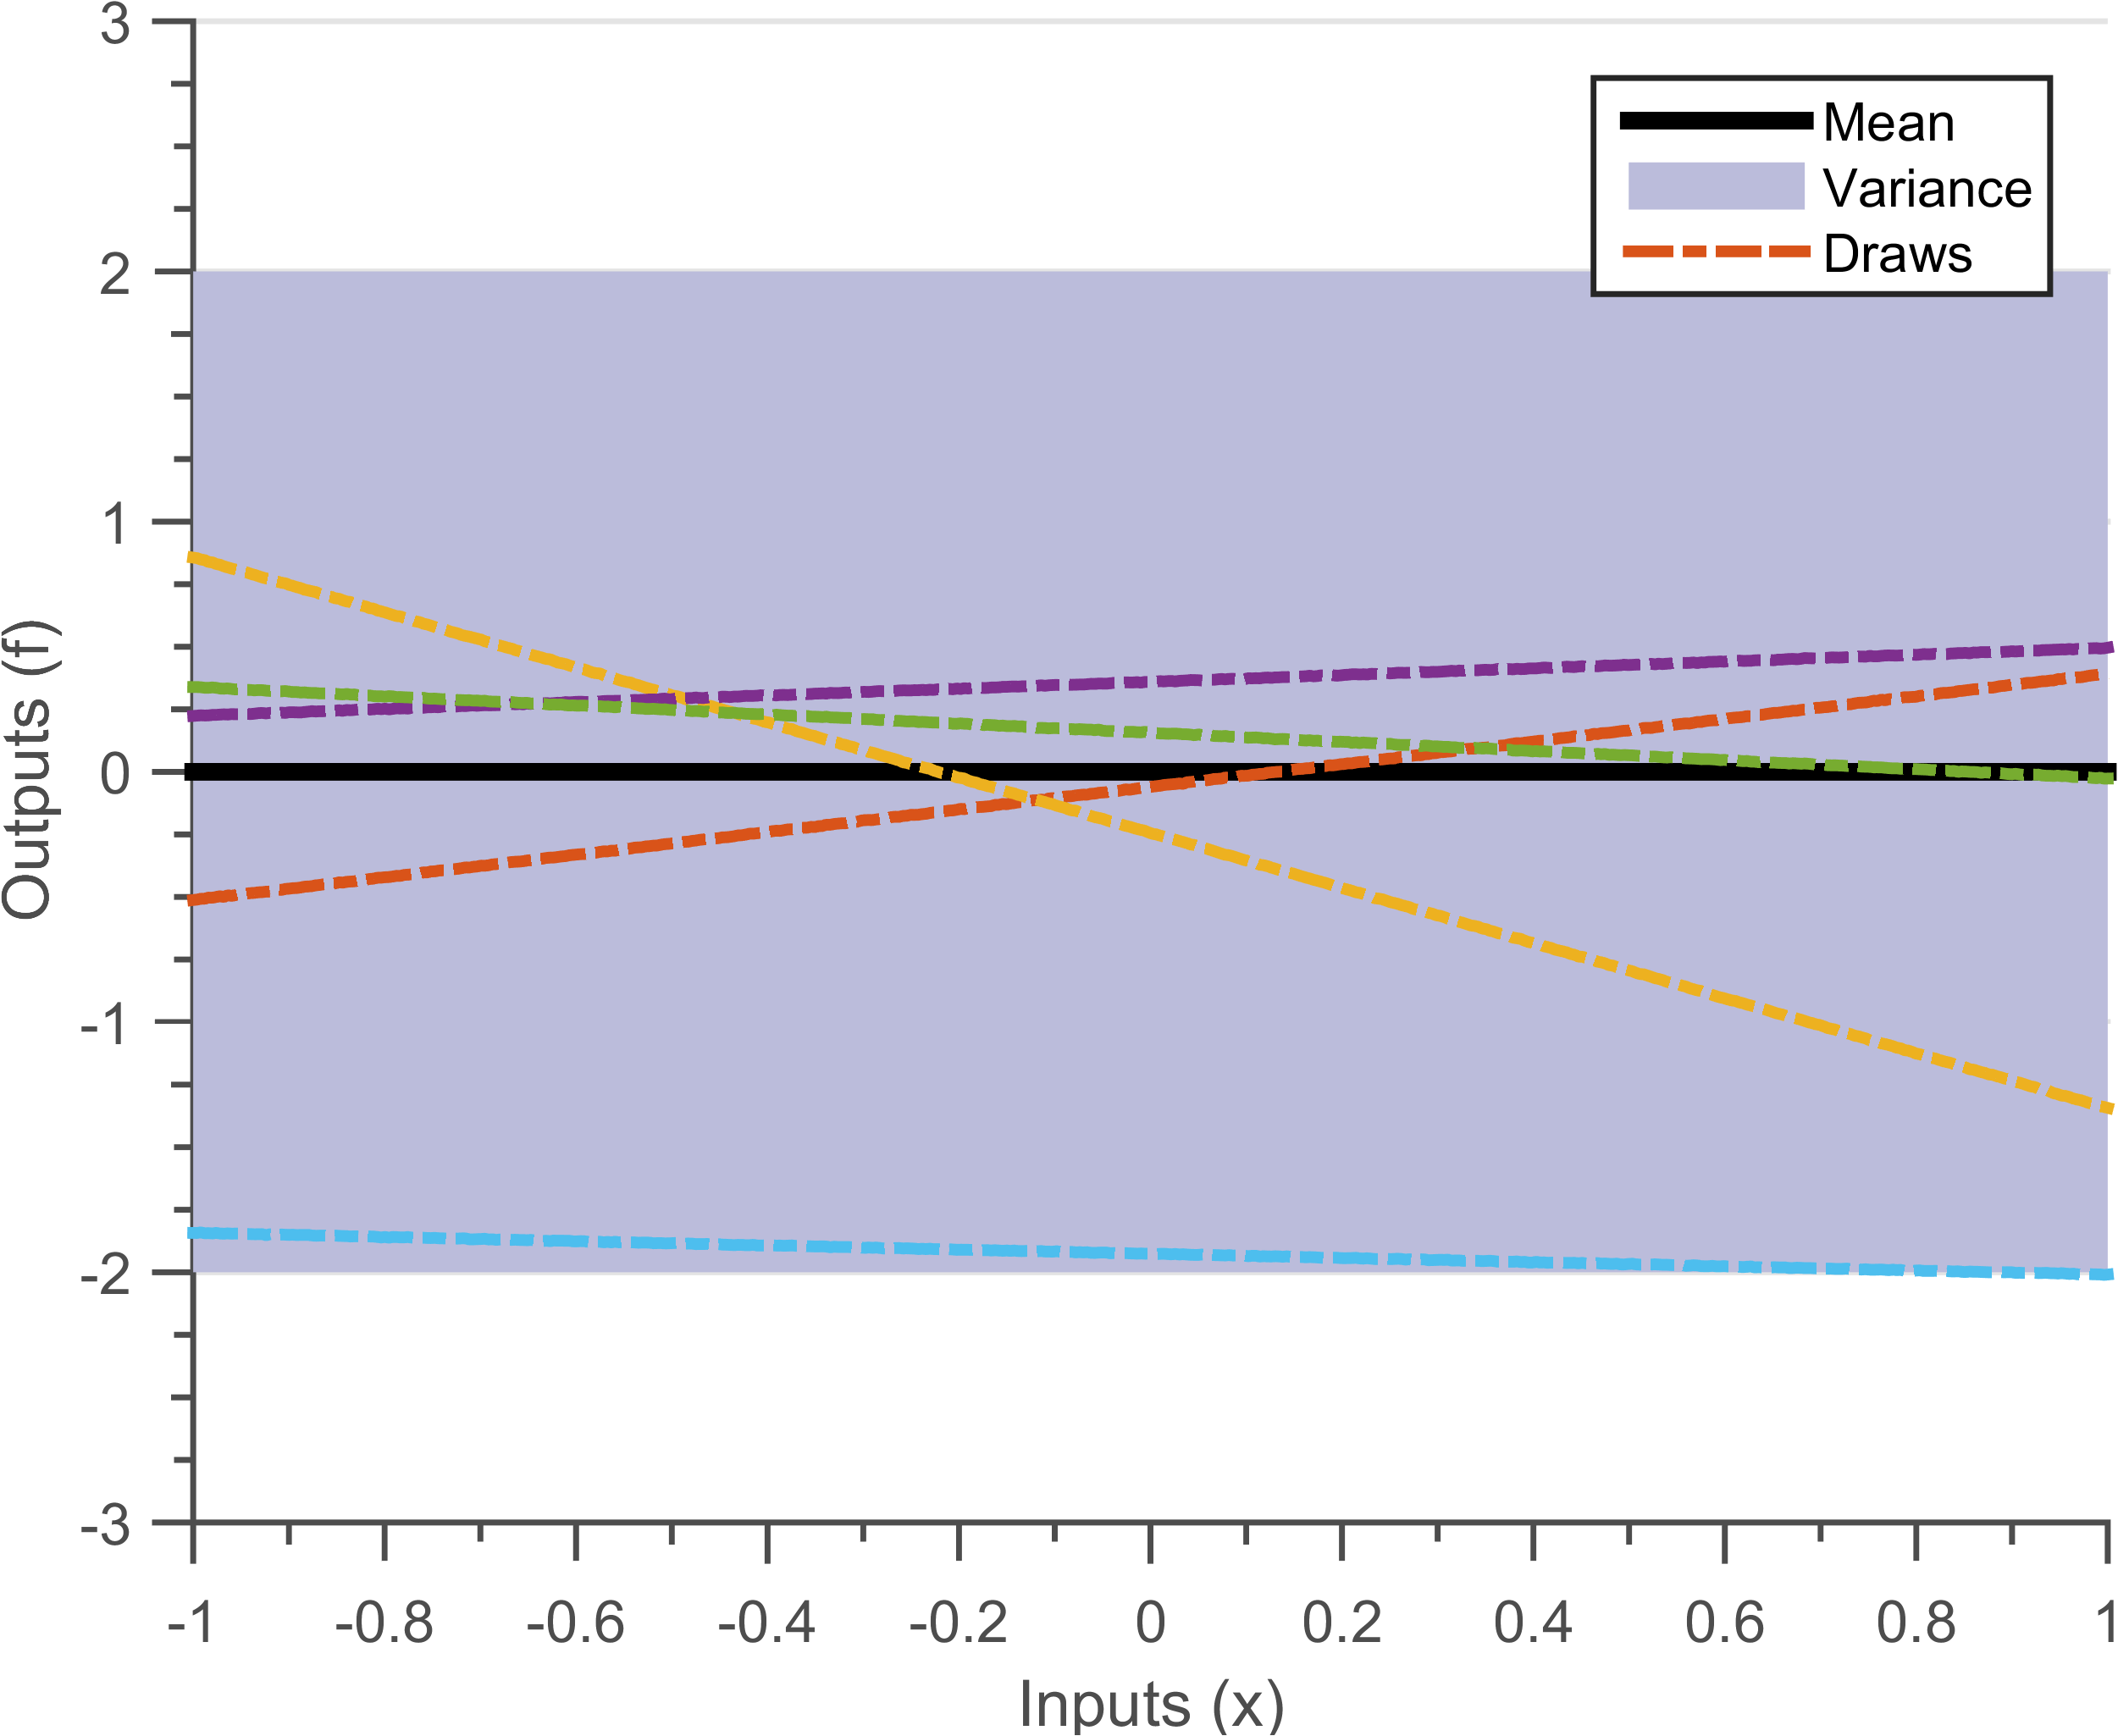
\includegraphics[width=0.45\textwidth]
        {imagesPart2/drawsLinear}
        \label{subFigdrawsLinear}
  }\quad
\subfigure[{Draws from a GP posterior with mean zero and Linear kernel (figure \ref{subFigdrawsLinear}) conditioned on the data \(X = -0.5, Y = 0\). The solid black line defines the mean function, shaded blue region defines 95\% confidence interval (2\(\sigma\)) distance away from the mean. The dashed lines are five functions drawn at random from a GP prior. The posterior mean passes from the data point, random functions drawn from a linear GP are linear}]
  {
        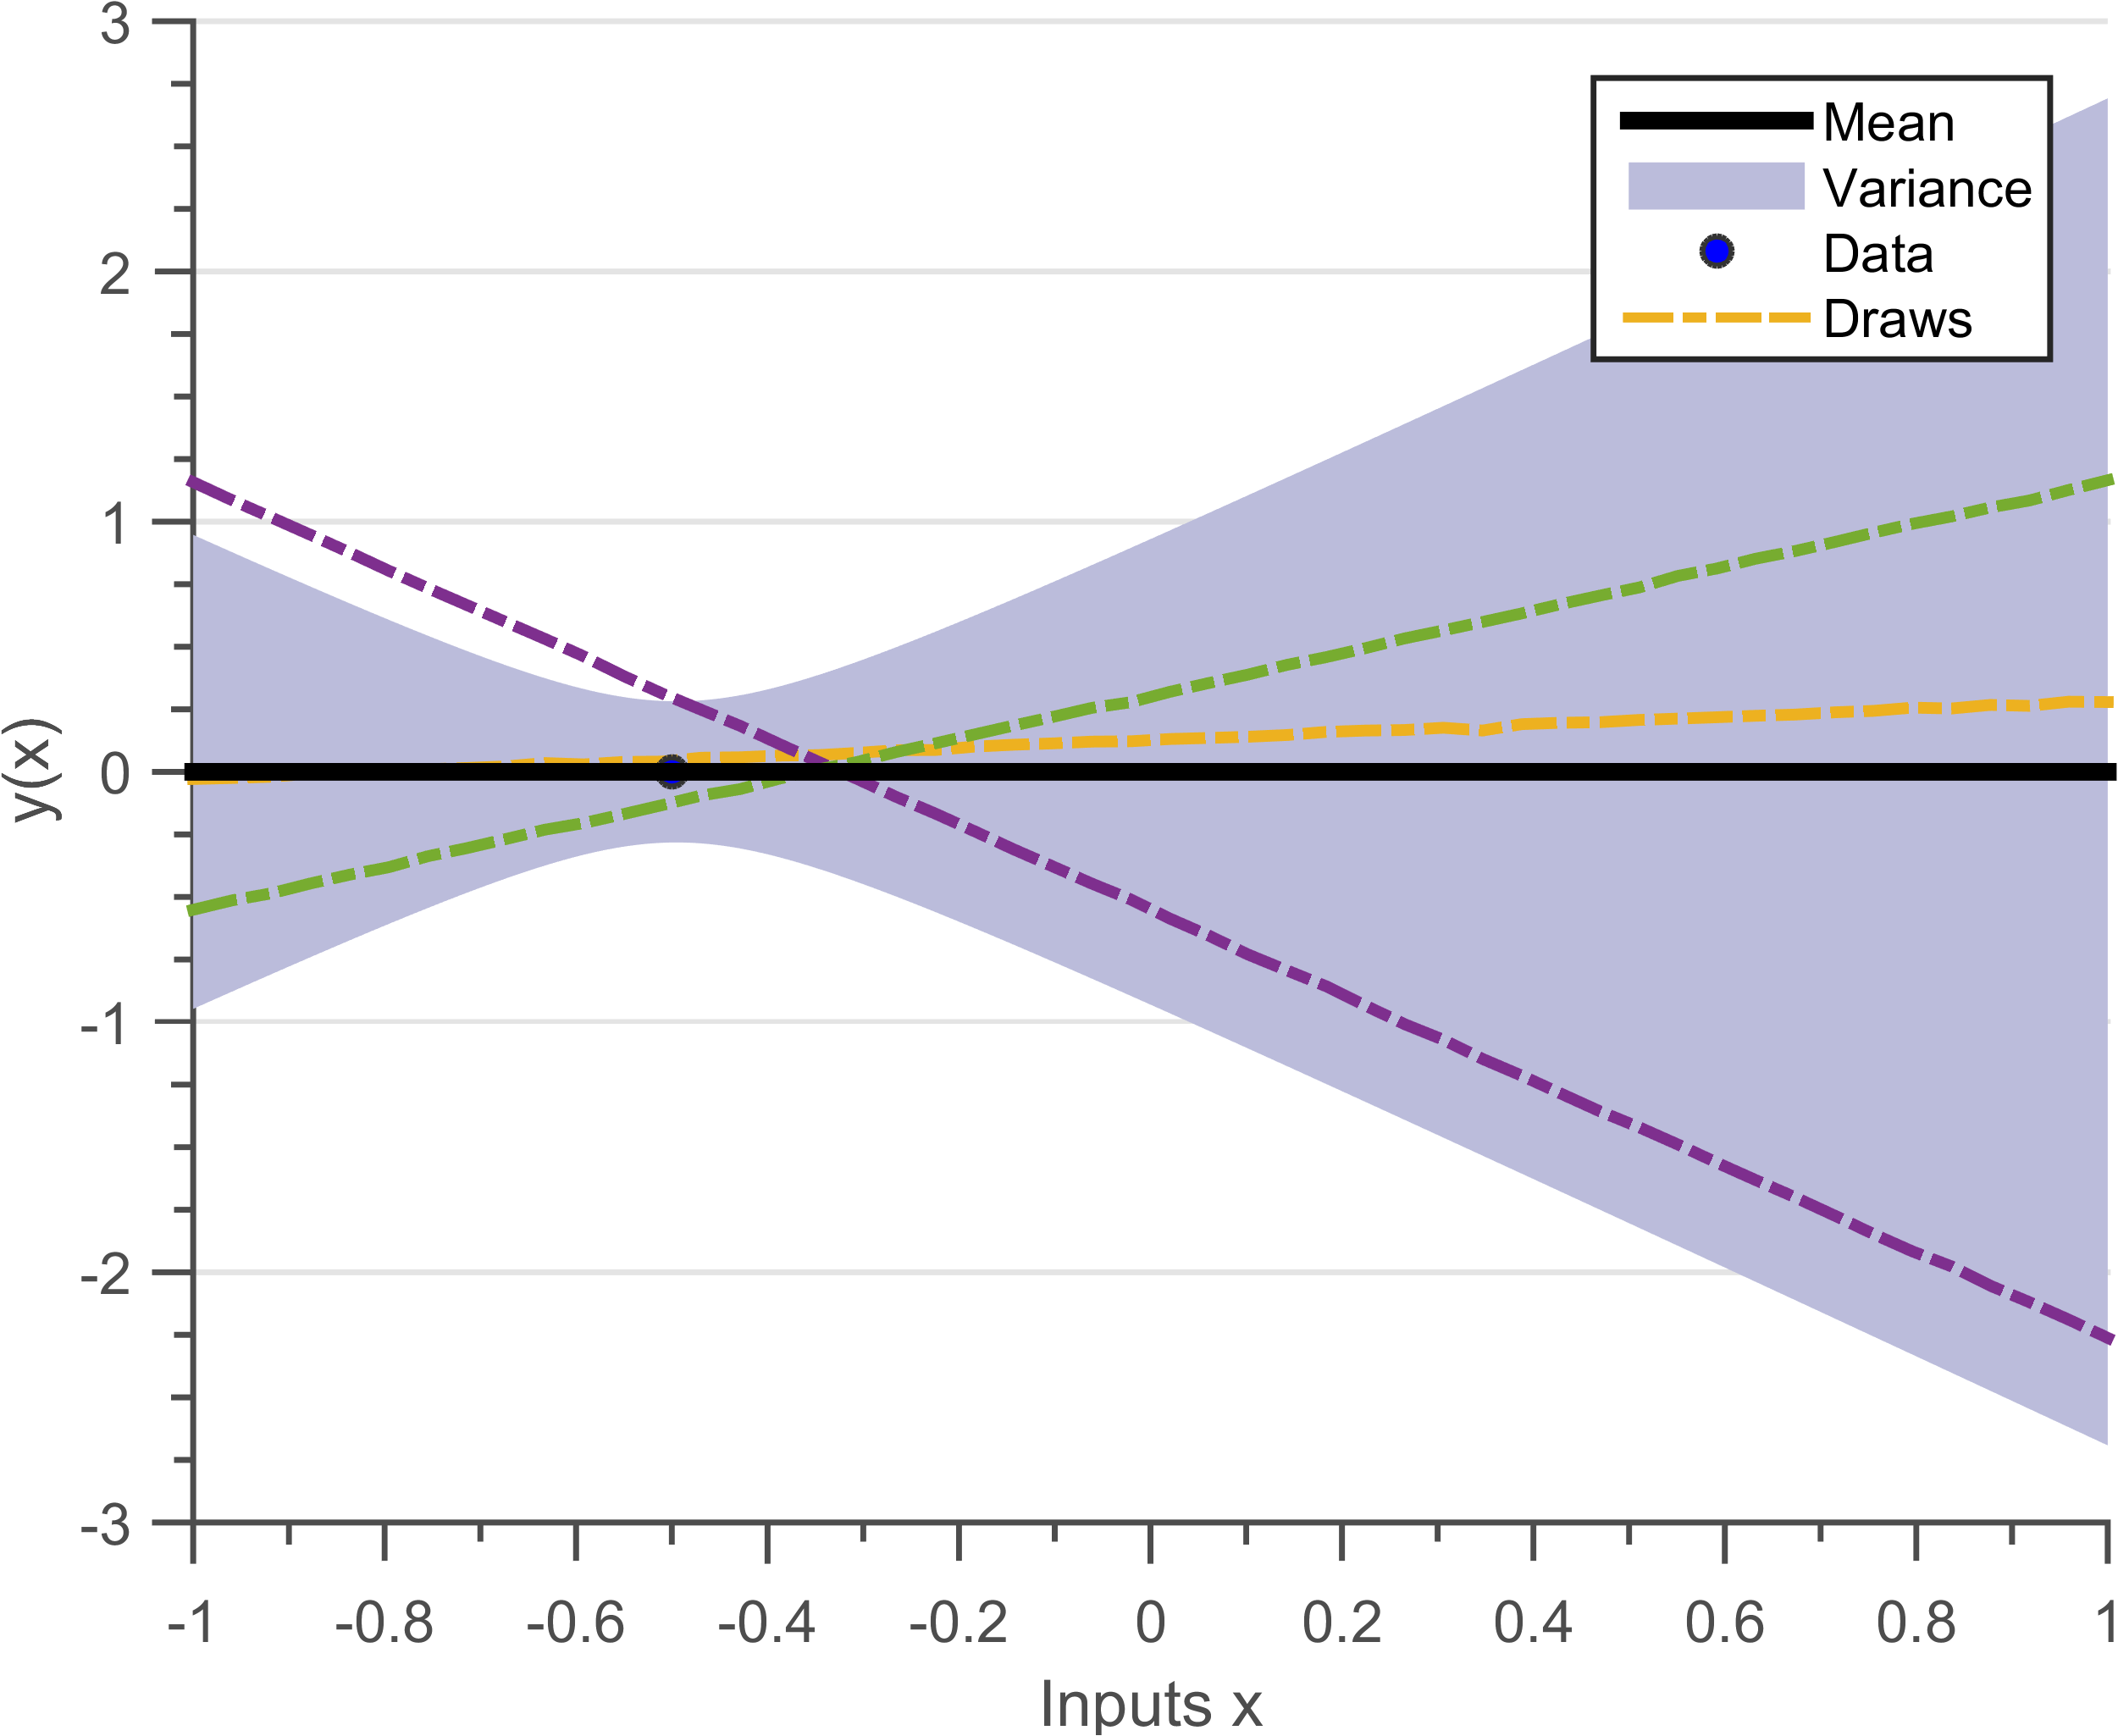
\includegraphics[width=0.45\textwidth]
        {imagesPart2/posteriorLinearNoisy_1}
        \label{subFigposteriorLinearNoisy_1}
  }\quad

       \caption{Prior and posterior from a GP prior of linear kernel}
       \label{figPriorAndPosteriorLinearKernel}
\end{figure}

Figure \ref{subFigmaximizingMarginalLikelihoodLinear} shows the contours of marginal likelihood with respect to \(w\). The marginal likelihood is maximum for \(w_{0} = 0.2576, w_{1} = 0.4584\), incidentally the same as posterior predictions in section \ref{toyDataSet1}. This means that the data has the highest possibility of coming from a dataset defined by such a prior. Figure \ref{subFigoptimizedPosteriorLinearNoisy_3} shows the posterior for same data set but for the hyper-parameters where marginal likelihood is maximum.

\begin{figure}[!ht]
  \centering
    \subfigure[{Marginal likelihood contours for varying bias and slope parameter. The noise hyper parameter is \((\sigma_{1} = [0.1])\). Marginal likelihood is maximum for \(w_{0} = 0.2576, w_{1} = 0.4584\).}]
  {
        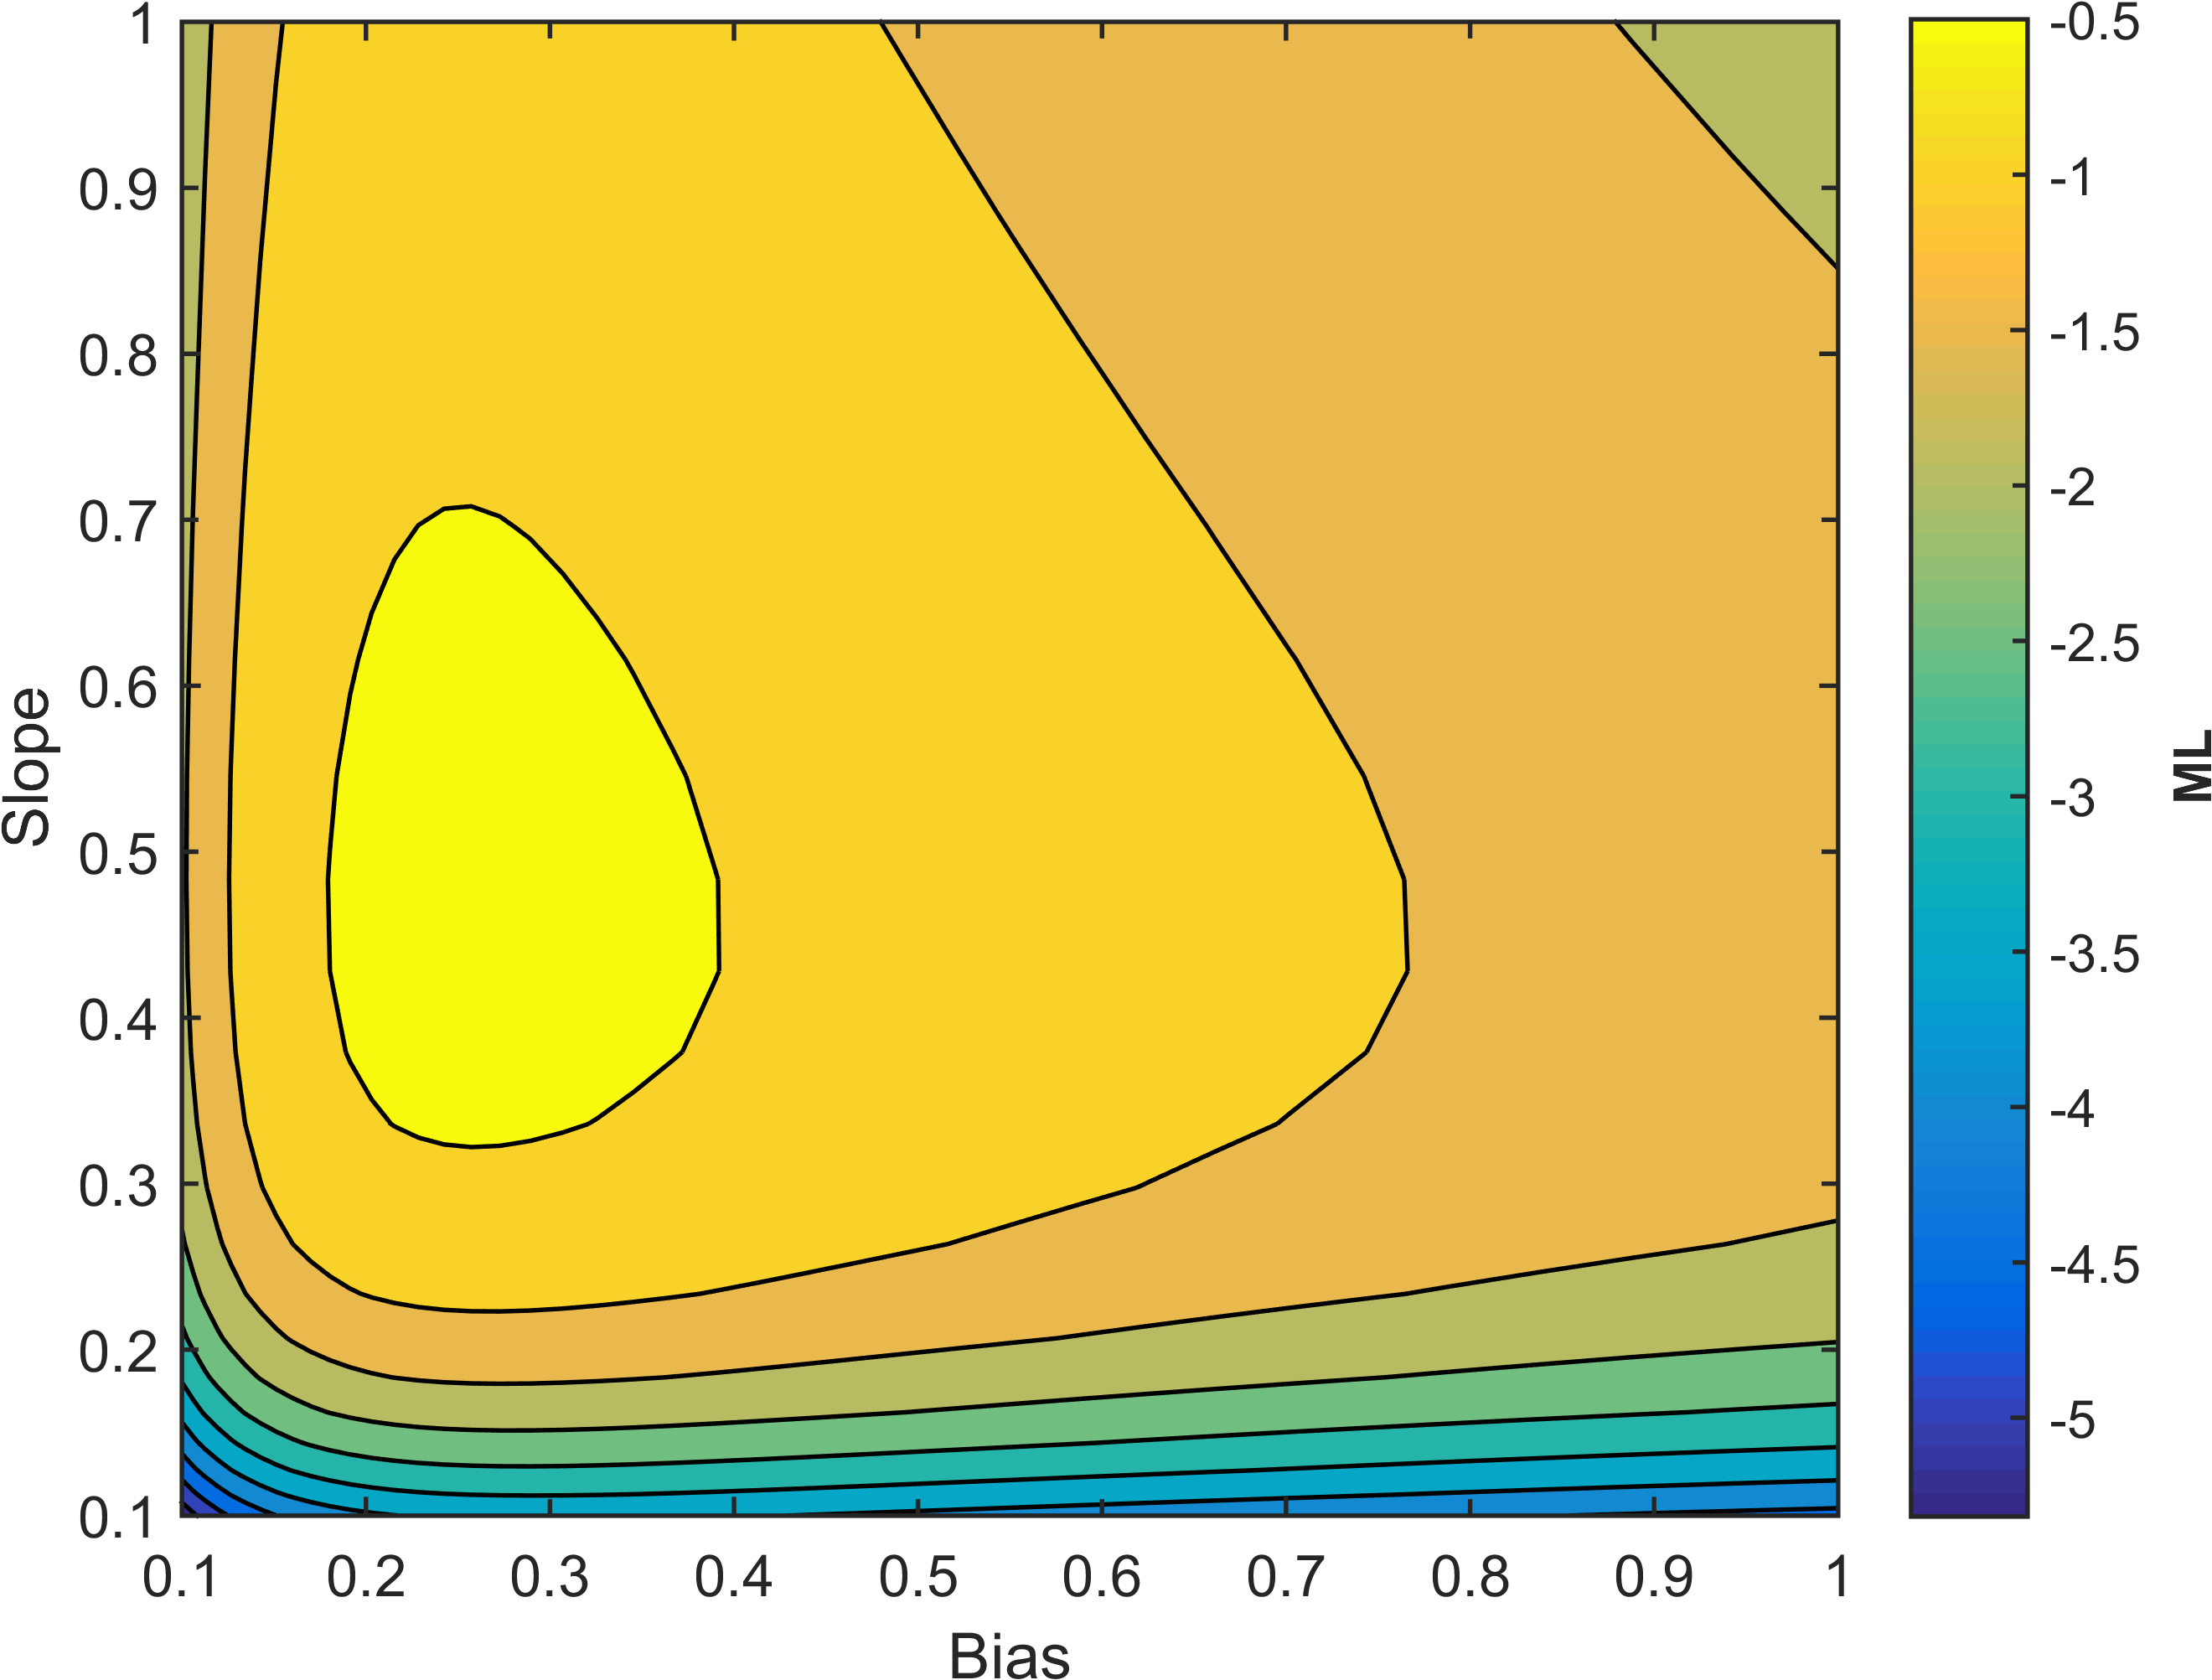
\includegraphics[width=0.45\textwidth]
        {imagesPart2/maximizingMarginalLikelihoodLinear}
        \label{subFigmaximizingMarginalLikelihoodLinear}
  }\quad
\subfigure[{Draws from a GP posterior, conditioned on the dataset \(\mathcal{D}_{1}\) with mean zero and Linear kernel with hyper-parameters that maximize the marginal likelihood.}]
  {
        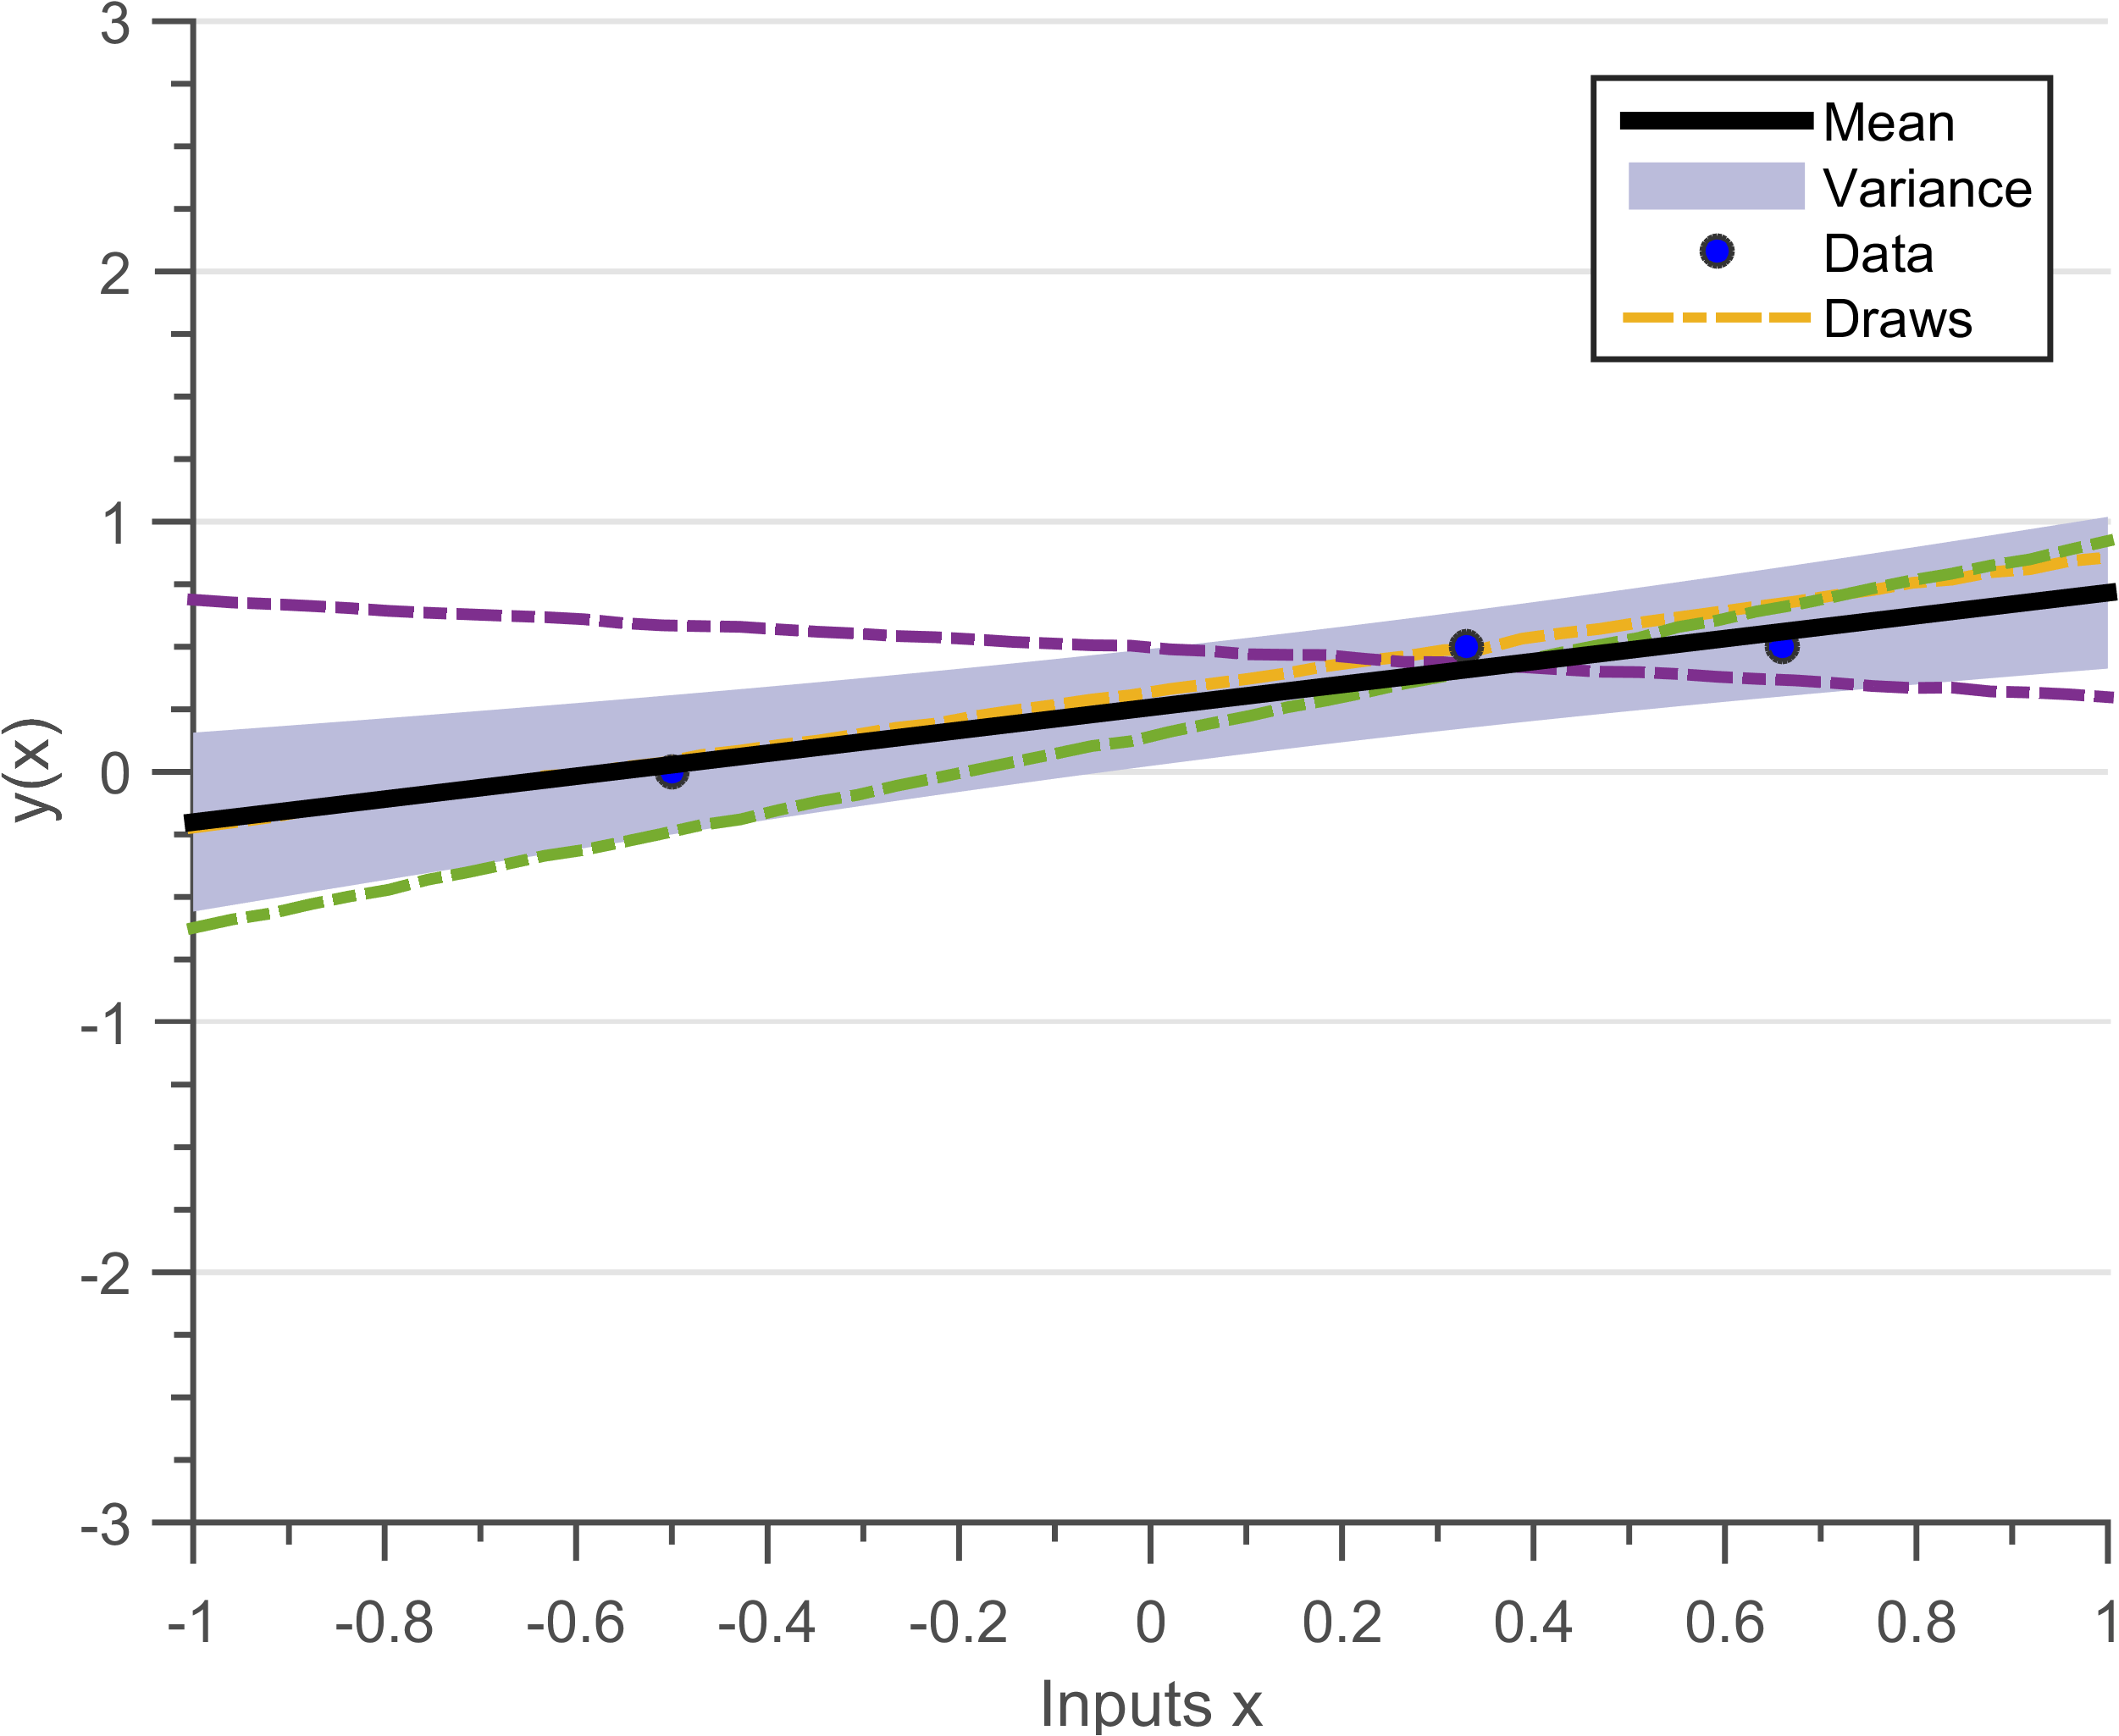
\includegraphics[width=0.45\textwidth]
        {imagesPart2/posteriorLinearNoisy_3}
        \label{subFigoptimizedPosteriorLinearNoisy_3}
  }\quad

       \caption{Maximizing Marginal Likelihood Linear kernel}
       \label{figMaximizingMLLinearKernel}
\end{figure}

\subsection{Neural Network Kernel}\label{subSecCh4NNkernel}
It can be shown that a neural network with infinitely many hidden units and an error activation function (\(erf(z)\) tends to a GP with a Neural network kernel \cite{neal2012bayesian, wilson2014covariance} (equation \ref{eqnNNKernel}). 

\begin{equation}\label{eqnNNKernel}
K_{NN}(x, x', \theta) = \theta_{1}^{2}\frac{2}{\pi} sin^{-1}\left ( \frac{2x\theta_{2}x'}{\sqrt{(1+2x^{T}\theta_{2}x)(1+2x'^{T}\theta_{2}x')}} \right )
\end{equation}

The hyperparameters \((\theta = [\theta_{1}, \theta_{2}])\) are; amplitude \(\theta_{1}\) which defines average distance from mean and the length scale \(\theta_{2}\) which define the smoothness of functions. GP with this covariance function defines a space of superimposed sigmoidal functions. We can use this kernel to embed the information of discontinuity in our family of functions. Figure \ref{figNNPrior} shows random draws from a Neural Network kernel but varying value of hyper parameters. Figure \ref{subfig:drawsNN100} has a higher value of \(\theta_{2}\) than figure \ref{subfig:drawsNN10}, which makes the constituent functions have stronger slope.

\begin{figure*}[!ht]
  \centering
  \subfigure[{Draws from a GP prior with mean zero and Neural Network kernel (equation \ref{eqnNNKernel}) with \(\theta = [1, 10]\).}]
  {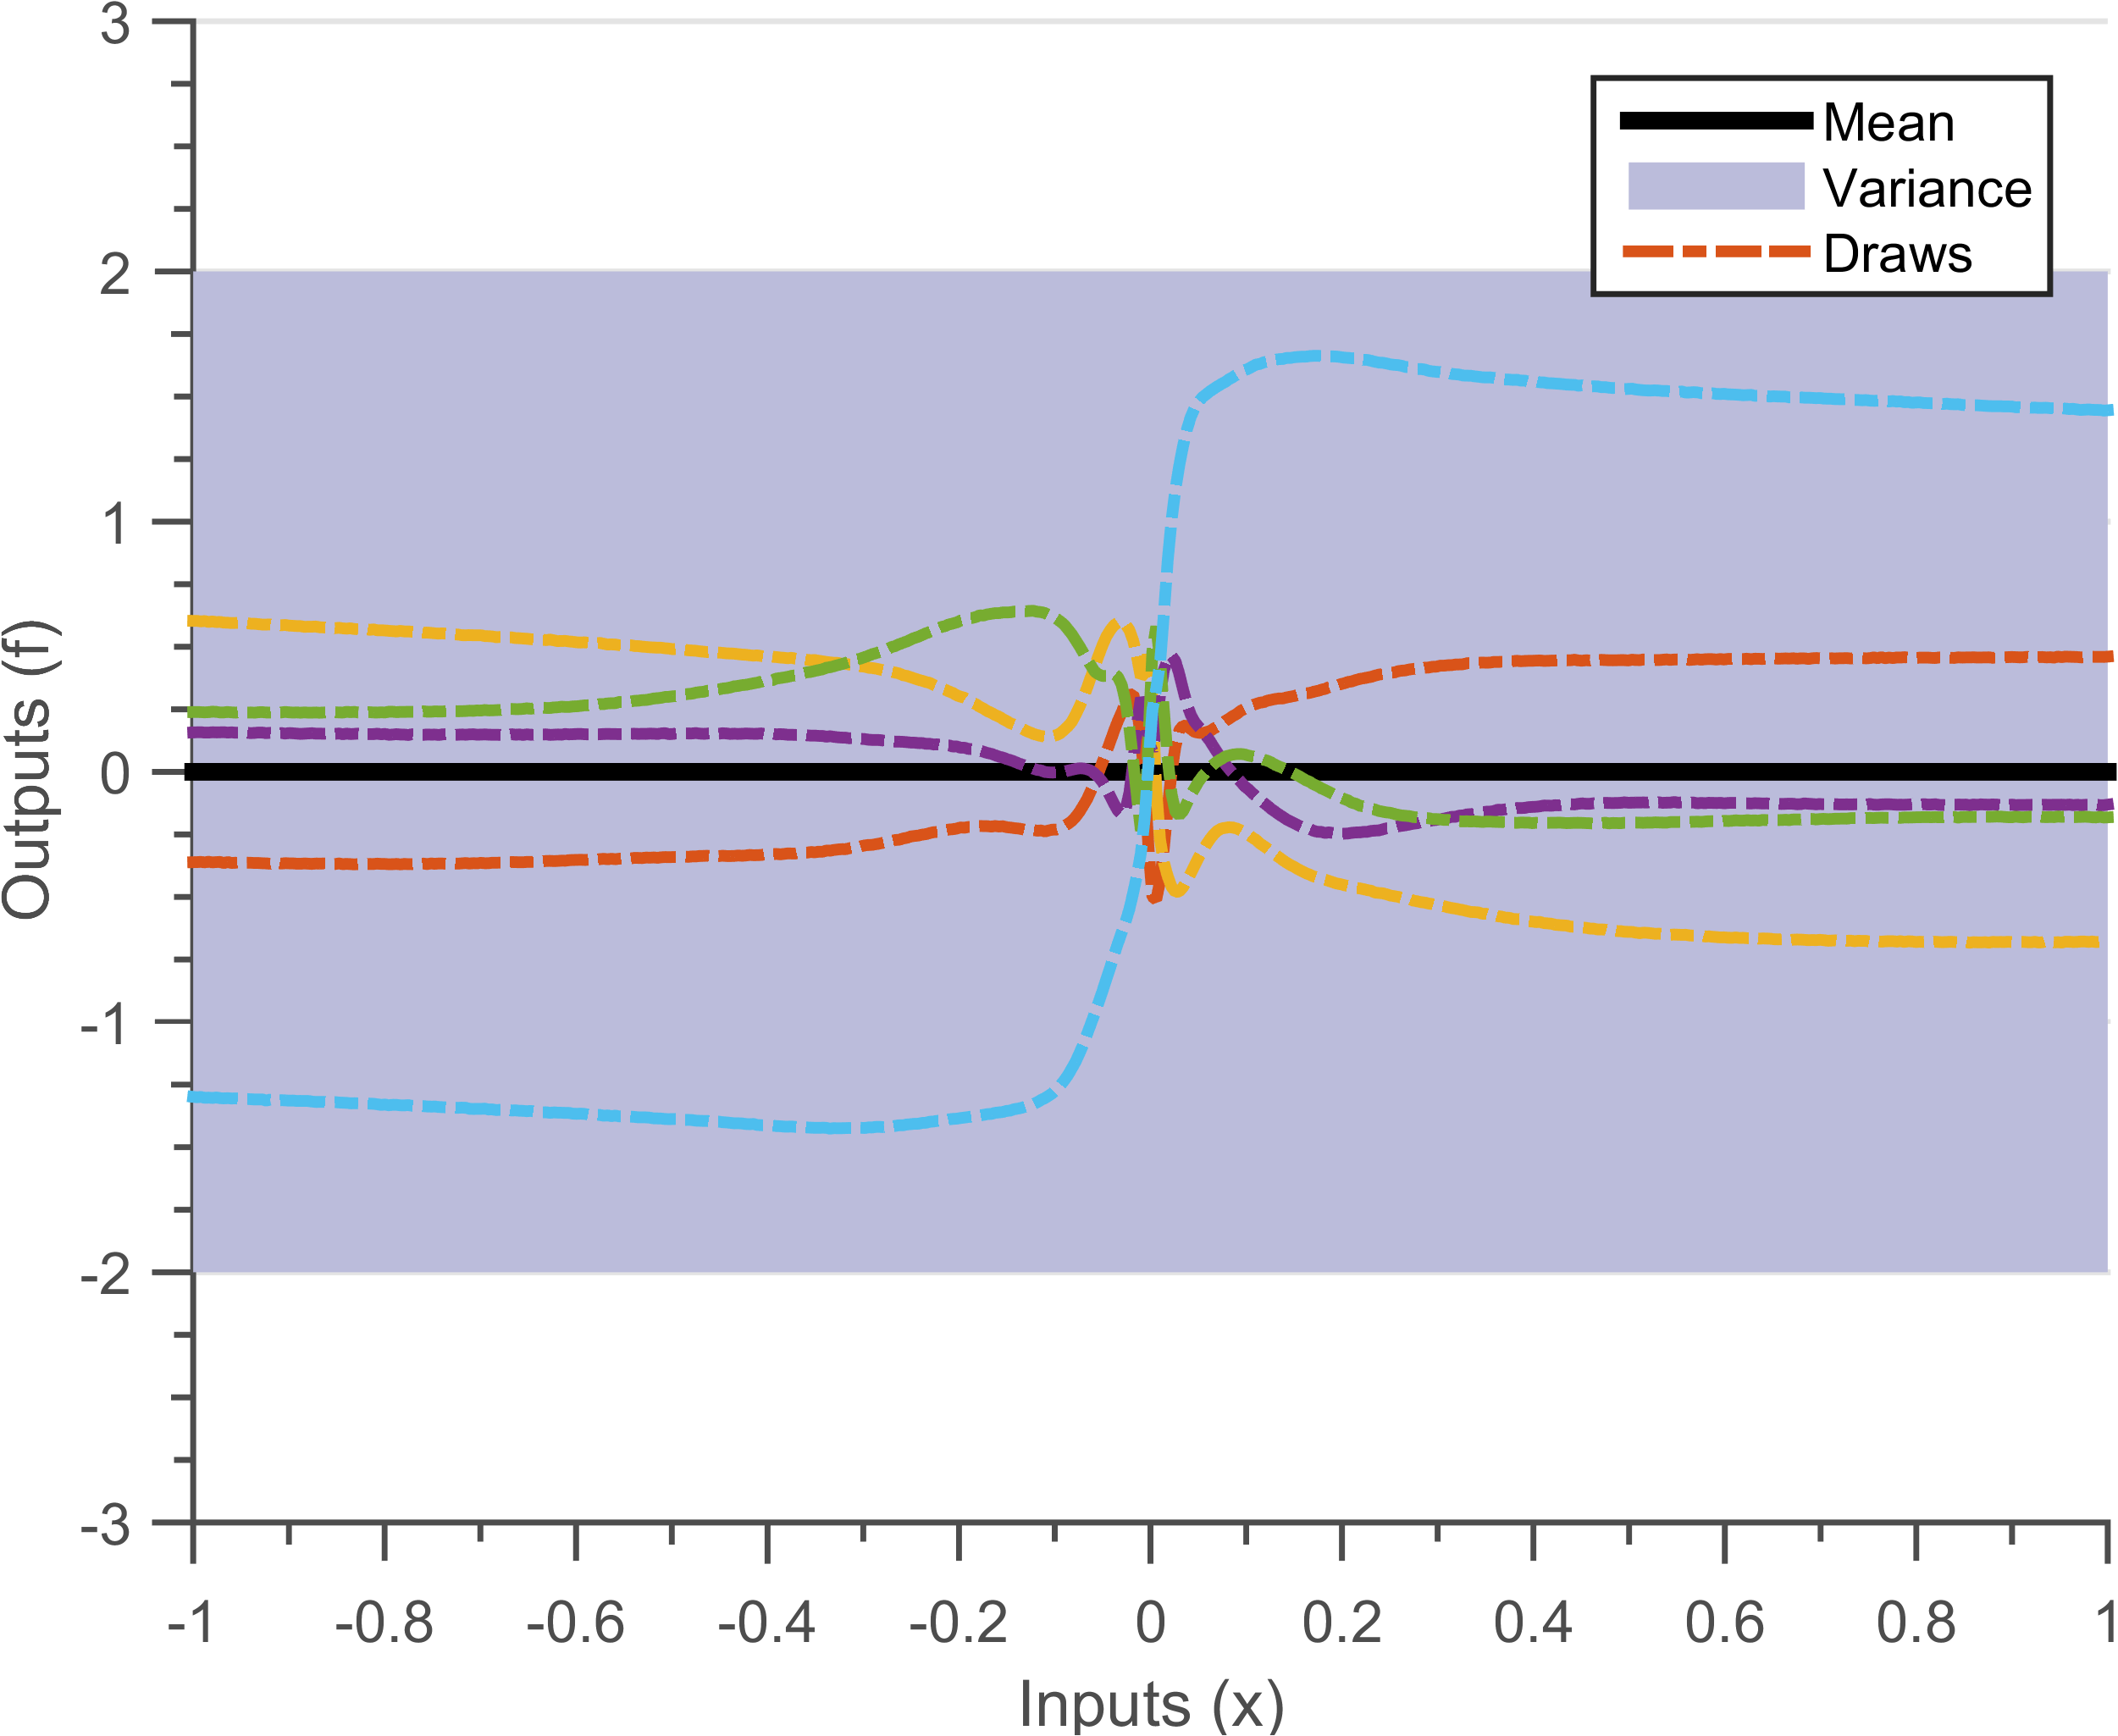
\includegraphics[width=0.45\textwidth]{imagesPart2/drawsNN10}\label{subfig:drawsNN10}}\quad
    \subfigure[{Draws from a GP prior with mean zero and Neural Network kernel (equation \ref{eqnNNKernel}) with \(\theta = [1, 100]\). Higher value of \(\theta_{2}\) signifies increasing slope}]
  {\includegraphics[width=0.45\textwidth]{imagesPart2/drawsNN100}\label{subfig:drawsNN100}}\quad
  \caption{Draws from Neural Network kernels having different hyper-parameters. The solid black line defines the mean function, shaded blue region defines 95\% confidence interval (2\(\sigma\)) distance away from the mean. The dashed lines are five functions drawn at random from a GP prior.}
  \label{figNNPrior}
\end{figure*}

\subsection{Change-Point kernels}\label{subSecCh4CPKernel}
Changepoint (CP) kernels can be defined through addition and multiplication with sigmoidal functions. They were introduced to identify changepoints in time-series modelling \cite{osborne2010bayesian}. This kernel expresses a change from one form of structure to another. 
\begin{equation} \label{eq:changePointKernel}
CP(k_{1}, k_{2}(x, x')) = sigm(x)k_{1}sigm(x') + (1-sigm(x))k_{2}(1-sigm(x'))
\end{equation}

The parameters of the sigmoidal determine the steepness of the changepoint and the placement of changepoint.


\begin{figure*}[!ht]
  \centering
  \subfigure[{Draws from a GP prior with mean zero and CP kernel (equation \ref{eq:changePointKernel}) between a Linear and a SE kernel with \(\theta_{CP} = [1, 0]\).}]
  {\includegraphics[width=0.29\textwidth]{imagesPart2/drawsCP1}\label{subfig:drawsCP1}}\quad
    \subfigure[]
  {\includegraphics[width=0.29\textwidth]{imagesPart2/drawsCP10}\label{subfig:drawsCP10}}\quad
  \subfigure[]
  {\includegraphics[width=0.29\textwidth]{imagesPart2/drawsCPMinus10}\label{subfig:drawsCPMinus10}}\quad
  \caption{}
\end{figure*}

\subsection{Application: Identifying onset of non-linearity  using CP kernel}\label{subsubsecCh4ApplicationCP}
In several physical processes, there is an equilibrium condition. Near this equilibrium, a linear approximation is performed and when the assumptions start failing a non-linear domain is observed. This basic approximation is made in experiments such as: lift vs alpha curves; estimation of Young's Modulus; basics of control theory. The value of these physical parameters slope (eg. Young's Modulus) and position of changepoint (eg. plasticity) are progressively fed into further simulations. 

These basic physical properties define the general characteristics of the field. The parameters are then later fed into more complex designs and used as an input into particular mesh elements (remember induction vs deduction \ref{sec:machineLearning}). The values of slopes and position of change-point are approximated by engineering judgement. 

\begin{figure}[!ht]
  \centering
    \subfigure[]
	    {\includegraphics[width=0.45\textwidth]{imagesPart2/clAlphaCovCP}\label{subfig:clAlphaCovCP}}\quad
    \subfigure[]
	    {\includegraphics[width=0.45\textwidth]{imagesPart2/stressStraincovCPPlot}
	    \label{subfig:stressStraincovCPPlot}}
	    \caption{}
\end{figure}


We tried to solve the problem of estimating the lift coefficient using Gaussian Process. Using the changepoint kernel which transitions from linear domain (linear kernel) to non-linear domain (SE kernel), prior assumptions of the problem were encoded in the kernel structure. Open source data for the lift vs alpha curves for the NACA 0012 airfoil were chosen. Fig: \ref{subfig:clAlphaCovSE} shows the regression of the data using SE kernel. Fig: \ref{subfig:clAlphaCovCP} regression of the same dataset using the CP(linear, SE) kernel. 

We can observe that the algorithm predicts a changepoint for the dataset. This is the point with where the linear assumptions start failing, according to prior information. The marginal likelihood of CP(linear, SE) kernel is rigged with many local minimas. The algorithm tries to put a changepoint at every observation point. Hence using a global optimizer is advised. The changepoint kernel is also very numerically unstable hence cross-validating the learners is also very important (model ensembles \ref{subsec:modelEnsembles}). The results of this study will be presented in the SIAM Uncertainty Quantification 2016 Conference.


\section{Discussion}

\textbf{A table to list common  }
%%% Local Variables: 
%%% mode: latex
%%% TeX-master: "isae-report-template"
%%% End: 


\chapter{Combining Basic Covariance Functions}
\label{chapCombiningBasicCovariances}

What if the kind of pattern that we wish to encode is not captured by using the basic kernels (chapter \ref{chapBasicCovarianceKernels})? What if we wish to encode several different patterns in our hypothesis space? Or what if, we want to build models for data sets with more than one input dimension? Thankfully, several other kernels can be constructed with desired properties by merging the earlier mentioned basic covariance functions. 

Again the possible combinations of kernels described in this chapter are already known in the machine learning literature, but missing while applied to engineering design models.The original contribution of this chapter is to apply the newly created covariance functions to create models. Below are a few simple techniques to create valid covariance functions, all these operations retain the positive definiteness of the covariance functions \cite{bishop2006pattern, mackay2003information, durrande2001etude, durrande2013anova}. . 



\begin{align}
k(x_{1}, x_{2}) =  & k_{1}(x_{1}, x_{2}) + k_{2}(x_{1}, x_{2})  \label{eqCh5AddingCovariances} \\
k(x_{1}, x_{2}) =  & k_{1}(x_{1}, x_{2}) \times k_{2}(x_{1}, x_{2}) \label{eqCh5MultiplyingCovariances} \\
k(x_{1}, x_{2}) =  & q(x_{1})k_{1}(x_{1}, x_{2})q(x_{2}) \label{eqCh5MultiplyingWithFunction} \\
k(x_{1}, x_{2}) =  & k_{1}(h(x_{1}), h(x_{2})) \label{eqCh5ComposedCovariances} \\
k(x_{1}, x_{2}) =  & g(g(k_{1}(x_{1}, x_{2}), x_{1}), x_{2} ) \label{eqCh5LinearOperatorCovariances}
\end{align}


Here, $k_{1}(x_{1}, x_{2})$ and $k_{2}(x_{1}, x_{2})$ are valid covariance function, while $q$ and $h$ are any continuous functions. Here $g\left ( . \right ) \in \mathcal{C}^{2}$ is an linear operator, for more discussion on equation \ref{eqCh5LinearOperatorCovariances} refer to chapter \ref{chapAddingEquationsInGP}. Let, us take the case for a 2-dimensional input vector $x$ such that $x = \{x^{1}, x^{2}\}$. Then the following covariance functions are also valid.

\begin{align}
k(x_{1}, x_{2}) = k_{1}(x_{1}^{1}, x_{2}^{1}) + k_{2}(x_{1}^{2}, x_{2}^{2}) \label{eqCh5AddingAcrossDimensionsCovariances} \\
k(x_{1}, x_{2}) = k_{1}(x_{1}^{1}, x_{2}^{1}) \times k_{2}(x_{1}^{2}, x_{2}^{2}) \label{eqCh5MultiplyingAcrossDimensionsCovariances} 
\end{align}

The current chapter is written to provide intuition on what happens when we combine several covariance functions. This chapter unfolds as follows; section \ref{secSingleDimension} provides intuition on combining kernels for one-dimensional inputs, while section \ref{secMultiDimensionalKernels} details how to create covariance functions for higher-dimensions (equation \ref{eqCh5AddingAcrossDimensionsCovariances} and \ref{eqCh5MultiplyingAcrossDimensionsCovariances}) inputs. 

\section{One dimensional inputs}\label{secSingleDimension}
Combining kernels can give rise to interesting features, in this section we provide intuition on combining kernels in one dimension. Section \ref{subsecStructureKernelsMultiplyingKernels} details of effects of multiplying kernels (equation \ref{eqCh5MultiplyingCovariances}) while section \ref{subsecStructureKernelsAddingKernels} describes effects of adding kernels (equation \ref{eqCh5AddingCovariances}). Section \ref{subsubsecCh4ApplicationCP} uses the equation \ref{eqCh5MultiplyingWithFunction} to describe a change-point kernel, we use a change-point kernel to detect start of plasticity in an elastic beam and start of flow separation on an airfoil \cite{chiplunkar:hal-01555401}. 

\textbf{For clarity, we now on denote a covariance function $k(x_{1}, x_{2})$ by removing the input pairs ($x_{1}, x_{2}$) as $k$.}
 

\subsection{Multiplying Kernels} \label{subsecStructureKernelsMultiplyingKernels}
Multiplying two covariance functions acts as an AND operator, the resulting kernel has high value only if we have high value on both the kernels. Multiplying a Linear kernel $T$ times will result in a $T^{th}$ order polynomial regression (equation \ref{eqCh4PolynomialCovariance}). 

\begin{equation}\label{eqCh4PolynomialCovariance}
k_{Lin} = w_{0} + w_{1}x_{1}x_{2} \quad k_{Poly} = \prod_{i=1}^{T} \left (w_{0}^{i} + w_{1}^{i}x_{1}x_{2} \right)
\end{equation}

Figure \ref{subFigPriorMultiLinSE} shows the prior obtained after multiplying a Linear and a SE kernel. The hyper-parameters of the linear kernel are $w_{0}=0$ and $w_{1}=1$, this means that there is no intercept and $k_{Lin}(x_{1}, x_{2}) = x_{1}x_{2}$. The hyper-parameters of the SE part are $\theta_{amplitude}=1$ and $\theta_{lengthScale}=1$, similar to figure \ref{subFigpriorDrawsSE}. This covariance function resembles a SE covariance function but with the amplitude hyper-parameter proportional to distance \(x\) (equation \ref{eqMultiLinSECovariance}). 

\begin{equation}\label{eqMultiLinSECovariance}
k_{Multi} = x_{1}x_{2} exp[- \frac{\tau^2}{2}]
\end{equation}

\begin{figure}[!ht]
  \centering
    \subfigure[{Draws from a GP prior with mean zero and kernel obtained by \textbf{multiplying} a Linear kernel with SE kernel. The hyper-parameters of the linear kernel are $w_{0}=0$ and $w_{1}=1$ while the hyper-parameters of the SE part are $\theta_{amplitude}=1$ and $\theta_{lengthScale}=1$. We see that the variance at $x=0$ goes to zero, since multiplication is an AND operation}]
  {
        \includegraphics[width=0.45\textwidth]
        {imagesPart2/drawsMultiLinSE}
        \label{subFigPriorMultiLinSE}
  }\quad
\subfigure[{Draws from a GP prior with mean zero and kernel obtained by \textbf{adding} a Linear kernel with SE kernel. The hyper-parameters of the linear kernel are $w_{0}=0$ and $w_{1}=1$ while the hyper-parameters of the SE part are $\theta_{amplitude}=1$ and $\theta_{lengthScale}=1$. We see that the variance at $x=0$ goes to variance of SE ekrnel, since multiplication is an OR operation}]
  {
        \includegraphics[width=0.45\textwidth]
        {imagesPart2/drawsSumLinSE}
        %\label{}
  }\quad

       \caption{Random draws from combining a Linear and SE kernel. The solid black line defines the mean function, shaded blue region defines 95\% confidence interval (2$\sigma$) distance away from the mean. The dashed lines are five functions drawn at random from a GP prior. Random functions drawn from a linear GP are linear.}
       \label{figPrior}
\end{figure}


\subsection{Adding Kernels} \label{subsecStructureKernelsAddingKernels}
Adding two kernels acts as an OR operator, this means that the resulting kernel will have high value if either of the two kernels have high value \cite{durrande2011additive}. 


Figure \ref{subFigPriorMultiLinSE} shows the prior obtained after adding a Linear and a SE kernel. The hyper-parameters of the linear kernel are $w_{0}=0$ and $w_{1}=1$, this means that there is no intercept and $k_{Lin}(x_{1}, x_{2}) = x_{1}x_{2}$. The hyper-parameters of the SE part are $\theta_{amplitude}=1$ and $\theta_{lengthScale}=1$, similar to figure \ref{subFigpriorDrawsSE}. 

An interesting consequence of adding kernels is that, now we can decompose the result into additive parts. Suppose $k_{Sum}$ is a covariance function by adding $n$ covariance functions $k_{1}, k_{2}, \ldots, k_{n}$ (equation \ref{eqCh5AddingCovariances}), then the posterior mean and covariance can be written as equation \ref{eqCh5PosteriorSumMean} and \ref{eqCh5PosteriorSumVariance}. 

\begin{align}\label{eqCh5PosteriorSumMean}
\mathbf{E}[f(x) \mid X, Y, k_{Sum}] = \sum_{i=1}^{n} K_{i}(x_{*}X)( K_{Sum}(X, X))^{-1}Y
\end{align}

\begin{equation}\label{eqCh5PosteriorSumVariance}
Cov[f(x) \mid X, Y, k_{Sum}] = \sum_{i=1}^{n} K_{i}(x_{*}x_{*}) - K_{i}(x_{*}X)( K_{Sum}(X, X) )^{-1}K_{i}(Xx_{*})
\end{equation}

This comes very handy while iteratively discovering structure in the data. In fact the noisy posterior case discussed in section \ref{figGPNoiseLessPosteriors} is a case of adding a SE kernel with a white noise kernel, a more complicated noise model can be created by adding several kernels together. \cite{Rasmussen2005} use a sum of several kernels to interpolate $CO_{2}$ content in the atmosphere through the years. \cite{automaticStatistician} propose to automatically detect pattern by iteratively adding new kernels until the posterior error variance represents a white noise . 

\subsection{Change-Point kernels}\label{subSecCh4CPKernel}
The changepoint kernel was introduced to recognize changes in regimes, and adapt the covariance function accordingly. They were initially introduced to identify changepoints in time-series modelling \cite{osborne2010bayesian, saatcci2010gaussian}. These kernels can be defined through addition and multiplication with sigmoidal functions (equation \ref{eqCh4SigmoidalFUnction}). 

\begin{align}
sigm(x, \theta) & = \frac{1}{\theta_{intensity} + e^{\theta_{changeLocation}-x}} \label{eqCh4SigmoidalFUnction} \\
CP(k_{1}, k_{2}, x_{1}, x_{2}) & = sigm(x_{1})k_{1}sigm(x_{2}) + (1-sigm(x_{1}))k_{2}(1-sigm(x_{2})) \label{eq:changePointKernel}
\end{align}

The hyper-parameters of this kernel are the $\theta_{changeLocation}$ which determines the place of the changepoint and $\theta_{intensity}$ determine the intensity of change between the two patterns. Figure \ref{figdrawsCP} shows the randomly drawn functions from a change point kernel for varying values of $\theta_{intensity}$, where the regime changes from a Linear kernel to a SE kernel. The hyper-parameters of the linear kernel are $w_{0}=0$ and $w_{1}=1$, this means that there is no intercept and $k_{Lin}(x_{1}, x_{2}) = x_{1}x_{2}$. The hyper-parameters of the SE part are $\theta_{amplitude}=1$ and $\theta_{lengthScale}=1$, similar to figure \ref{subFigpriorDrawsSE}. We see that as the value of $\theta_{intensity}$ increases the regime change happens more rapidly, while if $\theta_{intensity}$ changes sign then the order of regime changes from SE kernel to LInear kernel.

\begin{figure*}[!ht]
  \centering
  \subfigure[{Draws from a GP prior with mean zero and CP kernel (equation \ref{eq:changePointKernel}) between a Linear and a SE kernel with $[\theta_{intensity}, \theta_{changeLocation}] = [1, 0]$.}]
  {\includegraphics[width=0.29\textwidth]{imagesPart2/drawsCP1}\label{subfig:drawsCP1}}\quad
    \subfigure[{Draws from a GP prior with mean zero and CP kernel (equation \ref{eq:changePointKernel}) between a Linear and a SE kernel with $[\theta_{intensity}, \theta_{changeLocation}] = [10, 0]$. Notice if the value of $\theta_{intensity}$ increases then the change between two patterns becomes more significant.}]
  {\includegraphics[width=0.29\textwidth]{imagesPart2/drawsCP10}\label{subfig:drawsCP10}}\quad
  \subfigure[{Draws from a GP prior with mean zero and CP kernel (equation \ref{eq:changePointKernel}) between a Linear and a SE kernel with $[\theta_{intensity}, \theta_{changeLocation}] = [-10, 0]$. Notice if the sign of $\theta_{intensity}$ changes then the order of kernels gets reversed.}]
  {\includegraphics[width=0.29\textwidth]{imagesPart2/drawsCPMinus10}\label{subfig:drawsCPMinus10}}\quad
  \caption{Random draws by having a change-point between a Linear and SE kernel. The solid black line defines the mean function, shaded blue region defines 95\% confidence interval (2$\sigma$) distance away from the mean. The dashed lines are five functions drawn at random from a GP prior. Random functions drawn from a linear GP are linear.}
  \label{figdrawsCP}
\end{figure*}

\subsection{Application: Identifying onset of non-linearity  using CP kernel}\label{subsubsecCh4ApplicationCP}
Several physical processes can be represented using a linear approximation in some part of their regime. This approximation is possible because the linear effects dominate in that particular regime, but they eventually wear off and second and third order effects start becoming more powerful. 

This basic assumption is used in making simple models in several domains; for example in a material during the elastic regime $Stress \propto Strain$ is a basic linear approximation. The proportionality constant between Stress and Strain is called as the Young's Modulus, which is different for different materials. When the elastic regime starts wearing off, non-linear behaviour called plasticity starts taking over and the approximation $Stress \propto Strain$ is not valid anymore. Similarly in aerodynamics, when characterizing a flow over an airfoil during the Linear regime  $ Lift \propto Angle Of Attack$, the airflow is attached on the airfoil during this regime. When the airflow starts separating from the airfoil the linear effects start becoming less powerful and give rise to non-linear effects. 

The value of these basic physical parameters such as slope (eg. Young's Modulus, coefficient of lift) and position of change in regime (eg. start of plasticity and separation of flow) are progressively fed into further simulations. Generally, the slope and start of non-linearity are evaluated by engineering judgment, this is a painfully slow and costly process. 

We propose to estimate the slope and change-point automatically using GP and a change point kernel. Using the changepoint kernel which transitions from linear domain (linear kernel) to non-linear domain (SE kernel), prior information of the problem were encoded in the kernel structure. 

We perform our experiments of openly available Stress and Strain data of Aluminum Alloy 6061 \cite{kaufman1999properties} and Lift and Angle data of NACA 0012 airfoil\footnote{Airfoil data from: http://airfoiltools.com/airfoil/details?airfoil=n0012-il}. To estimate the change-point hyper-parameters we perform a 10-fold cross validation. The marginal-likelihood is optimized for the training dataset and change-point and slope of linear regime is noted. We then compare the mean slope with the values available in the literature. 

Table \ref{tabComparisonOfYoungModulus6061Data} shows the results of physical parameters for AL 6061 when calculated using change-point kernel vs that available in the literature. We can observe that the change-point automatically predicts the correct values of Young's Modulus and start of non-linearity.


\begin{table}[!h]
    \centering
\begin{tabular}{|l|l|l|}
  \hline
    & Change-point & Literature \\
  \hline 
  \hline
Young's Modulus (GPa) &  68.5 & 68.9\\
Start of plasticity  & 0.94\% & 0.95\%\\
   \hline
\end{tabular}
\caption{Comparison of Young's Modulus for Al 6061 data-set}
  \label{tabComparisonOfYoungModulus6061Data}
\end{table}

Figure \ref{figPosteriorChangePointKernel} shows the posterior predictions when using the changepoint kernel. Figure \ref{subfig:clAlphaCovCP} is the posterior distribution for the case of NACA 0012 airfoil, the Linear and SE regimes are plotted independently. Figure \ref{subfig:stressStraincovCPPlot} shows the posterior distribution for the case of AL 6061. We can observe that the algorithm predicts a changepoint for the dataset, this is the point where the non-linear effects start dominating. The marginal likelihood of a change-point kernel has many local minimas, there is a local minima at every observation point. This is because the kernel puts a non-linear regime at every observation point, hence a global optimizer should be used for optimization. The results of this study were be presented in the SIAM Uncertainty Quantification 2016 Conference \cite{chiplunkar:hal-01555401}.

\begin{figure}[!ht]
  \centering
    \subfigure[{Posterior distribution for the case of NACA 0012 airfoil, the Linear and SE regimes are plotted independently.}]
	    {\includegraphics[width=0.45\textwidth]{imagesPart2/clAlphaCovCP}\label{subfig:clAlphaCovCP}}\quad
    \subfigure[{Posterior distribution for the case of AL 6061 alloy, the Linear and SE regimes are plotted independently.}]
	    {\includegraphics[width=0.45\textwidth]{imagesPart2/stressStraincovCPPlot}\label{subfig:stressStraincovCPPlot}}
        \caption{Estimation of linear regimes using a change-point kernels}
        \label{figPosteriorChangePointKernel}
\end{figure}


\section{Multi-dimensional kernels}\label{secMultiDimensionalKernels}
In this section we develop intuitions on how to build kernels for higher-dimensional inputs. Section \ref{subSecLowDimensionalStructure} uses equation \ref{eqCh5ComposedCovariances} to encode lower-dimensional structure. We finally apply the multi-dimensional covariance function to interpolate aerodynamic pressure (section \ref{subecInterpolationOfAerodynamicPressures}), demonstrating the benefits of such an interpolating technique with common Proper Orthogonal Decomposition technique \cite{oatao18004}. Results of this exercise were used in a recent Airbus Flight Test campaign. 

Basic kernels can also be combined to create kernels for higher dimensions. Consider an input dataset which is multi-dimensional $x \in \mathbb{R}^{D_{inputs}}$. A simple additive kernel can be constructed by adding the kernels for individual dimensions \cite{hastie1990generalized}. This operation encodes the information that added dimensions are independent of each other (equation \ref{eq:SESum}). 

\begin{equation}\label{eq:SESum}
k(\tau, \theta) = \sum_{i=1}^{D_{inputs}} (\theta_{amplitude}^{i})^2 exp\left [ -\frac{(\tau^{i})^2}{2(\theta_{lengthScale}^{i})^2} \right ]
\end{equation}

Here, $\tau^{i} = x^{i}_{1} - x^{i}_{2}$ is the distance between two input points at the $i^th$ dimension. If we want to include interactions between two dimensions then their kernels can be multiplied together (equation \ref{eqCh5MultiplyingAcrossDimensionsCovariances}). A kernel which allows for interaction between all the possible $D_{inputs}$-dimensions can be constructed by multiplying all kernels for all the dimensions. The multi-dimensional Automatic Relevance Determination (ARD) kernel (equation \ref{eq:SEARD}) can be looked as a multiplication of several one-dimensional kernels with different length-scales \cite{Rasmussen2005}. It is called ARD because the value of length-scale determines which dimensions are more relevant.

\begin{equation}\label{eq:SEARD}
k(\tau, \theta) = (\theta_{amplitude})^2 \prod_{i=1}^{D_{inputs}}  exp\left [ -\frac{(\tau^{i})^2}{2(\theta_{lengthScale}^{i})^2} \right ]
\end{equation}

Figure \ref{figPrior2dimensional} shows a randomly drawn functions from a 2 dimensional kernel. Figure \ref{subFigdrawsProdMultiDimensional} is obtained after multiplying 2 SE kernels, while figure \ref{subFigdrawsSumMultiDimensional} is obtained after adding 2 SE kernels. The hyper-parameters of both the SE kernels are $\theta_{amplitude}=1$ and $\theta_{lengthscale}=0.2$ 

\begin{figure}[!ht]
  \centering
    \subfigure[{Random draw from a 2 dimensional prior obtained after \textbf{multiplying} two SE kernels. The hyper-parameters of both the SE kernels are $\theta_{amplitude}=1$ and $\theta_{lengthscale}=0.2$}]
  {
        \includegraphics[width=0.29\textwidth]
        {imagesPart2/drawsProdMultiDimensional}
        \label{subFigdrawsProdMultiDimensional}
  }\quad
\subfigure[{Random draw from a 2 dimensional prior obtained after \textbf{adding} two SE kernels. The hyper-parameters of both the SE kernels are $\theta_{amplitude}=1$ and $\theta_{lengthscale}=1$}]
  {
        \includegraphics[width=0.29\textwidth]
        {imagesPart2/drawsSumMultiDimensional}
        \label{subFigdrawsSumMultiDimensional}
  }\quad
\subfigure[{Random draw from a 2 dimensional prior obtained after \textbf{adding} two SE kernels. The hyper-parameters of both the SE kernels are $\theta_{amplitude}=1$ and $\theta_{lengthscale}=1$}]
  {
        \includegraphics[width=0.29\textwidth]
        {imagesPart2/drawsLowMultiDimensional}
        \label{subFigdrawsLowMultiDimensional}
  }\quad

       \caption{Random draw from a 2 dimensional prior.}
       \label{figPrior2dimensional}
\end{figure}

\cite{duvenaud2011additive, durrande2013anova} define a class of additive kernels which are formed upon adding several low-dimensional interactions. These kinds of kernels can be used to determine the important interactions and relevant dimensions.

The infinitely smooth assumption of the squared exponential function is unrealistic in several cases \cite{stein2012interpolation}, making the Mat\'ern kernels second most popular choice of kernels. Mat\'ern kernels have been found to have superior performance on datasets with high-dimensions \cite{le2013fastfood}. It is argued that the Mat\'ern kernel accounts for the concentration of measure effect in higher-dimensions. Imagine a high-dimensional orange (it is tough to imagine more than 3 dimensions), but if there was a high dimensional orange than most of its mass will be concentrated in its skin and not its pulp \cite{domingos2012few}. 

\subsection{Low dimensional structure}\label{subSecLowDimensionalStructure}
We can encode a low dimensional structure into family of functions by specifying the kernel as $k_{low} = k(Hx_{1}, Hx_{2})$ (equation \ref{eqCh5ComposedCovariances}), here $H$ is a low rank matrix. 


\begin{align}\label{eq:SELowDimensional}
k_{low}(\tau, \theta) = (\theta_{amplitude})^2  exp\left [  -\frac{1}{2}\tau\Sigma\tau^T \right ] 
\end{align}

Here, $\Sigma$ is $HH^T$ which encodes the low dimensional structure, when $\Sigma$ is a diagonal matrix we get a ARD kernel\footnote{$k(\tau, \theta) = (\theta_{amplitude})^2  exp\left [  -\frac{1}{2}\tau\Sigma\tau^T \right ] = (\theta_{amplitude})^2  exp\left [ \sum_{i=1}^{D_{inputs}} -\frac{(\tau^{i})^2}{2(\theta_{lengthScale}^{i})^2} \right ] 
= (\theta_{amplitude})^2 \prod_{i=1}^{D_{inputs}}  exp\left [ -\frac{(\tau^{i})^2}{2(\theta_{lengthScale}^{i})^2} \right ]$}. When the number of dimension increases significantly, the number of hyper-parameters also increases this makes the optimization of marginal likelihood inefficient. \cite{bouhlel2016optimisation} propose to use the strategy of encoding low dimensional information as a means to effectively reduce the number of hyper-parameters.

In the current section we have seen how to build covariance functions for multi-dimensional inputs. We now apply multi-dimensional kernels to build a surrogate model for Aerodynamics. We validate our method on 2 testcases: the first in subsonic regime on a Flap Track Fairing (FTF) and the second in transonic regime on NASA's Common Research Model (CRM) Wing. The results of these experiments were used during a recent Airbus FLight test campaign.

\subsection{Application: Interpolation of aerodynamic pressures}\label{subecInterpolationOfAerodynamicPressures}
Accurate prediction of aerodynamic pressures at a flight configuration is computationally expensive. Hence, it becomes advantageous to use surrogate models as approximations of high-fidelity aerodynamic models. A popular method of surrogate modelling in the aerodynamics community is by interpolating Reduced Order Models (ROM). A set of aerodynamic pressure snapshots is generated by performing CFD simulations for different aerodynamic parameters (eg. angle of attack $\alpha$, Mach). Then orthogonal basis vectors are found in the parameter space for the set of pressures snapshots. Generally, Proper Orthogonal Decomposition (POD) \cite{tan2003proper, rosenbaum2013efficient, braconnier2011towards} (also called as Principal Component Analysis (PCA) or Singular Value Decomposition (SVD)) is used to find the linear subspace. Finally, the reduced models are interpolated at the desired point in the parameter-space \cite{beckert2001multivariate, barrault2004empirical}. 

Due to the assumption of linear subspace, interpolation through ROM is highly efficient both in terms of cost and performance in the subsonic regime \cite{verveld2016reduced}. Unfortunately in the transonic regime, the shock creates a highly non-linear, almost discontinuous pressure distribution and the assumption of linear subspace does not hold \cite{li2016performance}. Although the performance of ROM interpolators can be improved with larger number of samples \cite{franz2014interpolation, forrester2008engineering}, we propose to improve the accuracy of prediction using distributd GP Regression for the same number of samples.  

Let us first start by defining a pressure snapshot. There exists a \(3\) dimensional spatial vector \(\omega_{i} \in  \mathbb{R}^{3}\) such that \(\omega_{i} = \{(\omega_{i}^{1}, \omega_{i}^{2}, \omega_{i}^{3})\}\). Here, \(i \in [1,N_{nodes}] \) are the spatial coordinates of the \(i^{th}\) pressure node in a CFD mesh containing \(N_{nodes}\) pressure nodes. Similarly there exists a \(D\) dimensional parameter vector \(d_{j} \in  \mathbb{R}^{D}\), for \(d_{j} = \{(d_{j}^{1}, d_{j}^{2}, \ldots ,d_{j}^{D})\}\). Here,   \(j \in [1,N_{parameter}] \) correspond to the \(j^{th}\) parameter set. The parameters can be any non-spatial parameter which are desired to be interpolated, some common examples include Mach, Angle of Attack for steady aerodynamics and time or frequency for unsteady aerodynamics. Since, this paper relates to interpolating steady aerodynamics \(d_{j}\) will correspond to the \(j^{th}\) CFD run in a total of \(N_{parameter}\) CFD simulations. 

The pressure measured on the \(i^{th}\) pressure node for the \(j^{th}\) parameter set will be denoted as \(p_{j}(\omega_{i})\) defined by the equation \ref{eq:pijSnapshot}. We next define the matrix \(\Omega = \{\omega_{1}; \omega_{2}; \ldots ; \omega_{N_{nodes}}\}\) for \(\Omega \in \mathbb{R}^{N_{nodes} \times 3}\) containing the full spatial information of the CFD mesh. Finally, the pressure snapshot for the CFD run \(j\) will be denoted as \(P_{j}(\Omega) = \{p_{j}(\omega_{1}); p_{j}(\omega_{2}); \ldots ; p_{j}(\omega_{N_{nodes}})\}\) for \(P_{j}(\Omega) \in \mathbb{R}^{N_{nodes}}\) defined by the equation \ref{eq:pressurefield}.

\begin{equation} \label{eq:pijSnapshot}
p_{j}(\omega_{i}) = CFD(\omega_{i}, d_{j})
\end{equation} 
\begin{equation}\label{eq:pressurefield}
P_{j}(\Omega) = CFD(\Omega, d_{j})
\end{equation} 

The POD methodology decomposes the set of pressure snapshots ($P_{j}(\Omega)$) into their eigen vectors ($\phi^{l}(\Omega)$) and participation factors ($a^{l}(d_{j})$). The pressure snapshots can now be reconstructed as a linear combination of its constituent eigen-vectors. To reconstruct the pressure snapshot at a new point $d_{new}$ the participation factors are interpolated and then linearly combined to give the new pressure snapshot (equation \ref{eq:interpPODEquation}). For more details please refer to appendix \textbf{reference to the appendix}

\begin{equation}\label{eq:interpPODEquation}
P_{new}(\Omega) = \sum_{l=1}^{p}a^{l}(d_{new}) \phi^{l}(\Omega)
\end{equation}

We now test the performance of distributed GP and POD+I on two sets of numerical experiments. Firstly, we test the accuracy on a detailed FTF design \cite{Bosco2016} in subsonic regime \ref{subSec:elsAResults} based on simulation from the elsA code \cite{cambier2008status}. Finally, we compare the accuracy on CRM wing in the transonic regime using elsA solver and kOmega-SST turbulence model \cite{vassberg2014summary}. 

elsA\textsuperscript{\textregistered} \cite{cambier2008status} is a pluri-function CFD simulation platform that allows representation of internal and external aerodynamics from the low subsonic to the high supersonic flow regime. Several formulations of the 3D Navier-Stokes equations can be chosen for arbitrary moving bodies. The GPML toolbox provided with \cite{rasmussen2006gaussian} is used to perform GP regression and distributed GP is inspired from \cite{deisenroth2015distributed}. The POD and interpolation analysis is done using built-in Matlab functions\cite{mathworks2005matlab}. All experiments were performed on an Intel quad-core processor with 4Gb RAM.

\subsubsection{Interpolation in subsonic regime}\label{subSec:elsAResults}
A FTF is situated below the wing and is used to deploy flaps for landing and take-off configurations. A FTF experiences heavy dynamic excitation due to the exhaust coming from engine. The dynamic nature makes the design of FTF a challenging task, where each simulation can last for 2 days. If we can effectively interpolate pressure snapshots then a 2 day dynamic simulation can be reduced to a few hours. 

Interpolation of FTF pressure snapshots has been earlier studied using POD methodology  \cite{bosco2016nonlinear}. In this section we use this dataset to validate the interpolation capabilities of distributed GP. 


\begin{figure*}[!ht]
  \centering
  \subfigure[Flap Track Fairing Pressure snapshot]
  {\includegraphics[height=0.15\textheight]{images/RANS_m6}\label{fig:ftf_snapshot}}\quad
  \subfigure[Flap Track Fairing DoF]
  {\includegraphics[height=0.15\textheight]{images/ftf_dof}\label{fig:ftf_dof}}\quad
      \caption{Details of the Flap track Fairing}
\end{figure*}


The FTF degree of freedom chosen for this analysis are $\theta$, the rotation around the longitudinal axis of the FTF, and $\alpha$ the rotation around the {\it spigot} axis, main connection between the track and the wing structure figure \ref{fig:ftf_dof}. The surface mesh of the CFD skin contains almost 36k nodes more precisely $N_{nodes} = 36802$. We run the simulation for 9 different values of $\alpha$ and 9 different values of $\theta$, more precisely we have run the CFD-Rans computation for $N_{parameter} = 9\times9 = 81$ number of times. In this particular case Reynolds Averaged  Navier-Stokes, {\it RANS}, equations are used with Spalart-Allmaras turbulence model to simulate the flow around the FTF. Figure \ref{fig:ftf_snapshot} shows one particular pressure snapshot. 

We use Leave One Out (LOO) Cross Validation method to quantify the performance of the two methodologies. $[\alpha, \theta]$ pairs are removed one by one from the database to create a new training set. The new training set is used to perform interpolation according to POD+I and distributed GP. Pressure snapshot is reconstructed for the missing $[\alpha, \theta]$ pairs. The methods are finally compared by evaluating the Root Mean Square Error (RMSE) and time of prediction values for each pair case. 

While performing distributed GP regression, we learn a GP model between $p_{ij}$ and input vector $X = [\omega_{i}^{1}, \omega_{i}^{2}, \omega_{i}^{3}, \alpha, \theta]$. We build a multi-dimensional kernel by multiplying 5 Mat\'ern kernels, different length-scale for each dimension. As discussed earlier we propose to use Mat\'ern kernel since the SE kernel has a very restrictive hypothesis space for high-dimensional regression.  Effectively we are learning a GP model for $N = 36802\times80 = 2.9$ million data-points. 

\begin{figure*}[!ht]
  \centering
  \subfigure[{Box plots of normalized RMSE for the two different model types. POD has a RMSE of $0.48\pm0.27$ whereas distributed GP has a RMSE of $0.37\pm0.1$. The mean distributed GP prediction is $20\%$ better than POD. Outliers are extrapolation cases }]
  {\includegraphics[width=0.45\textwidth]{images/rmse_AST}\label{subfig:RMSECFD}}\quad
    \subfigure[{Time taken to perform prediction for the two different model types. 
    POD takes $2.35s\pm0.11s$ whereas distributed GP takes $37.84s\pm4.35s$ to perform the interpolation. The average POD method is 19 times faster than distributed GP.}]
    {\includegraphics[width=0.45\textwidth]{images/time_AST}\label{subfig:timeCFD}}
  \caption{Results for elsA interpolation}
\end{figure*}

Figures \ref{subfig:RMSECFD} denote the RMSE estimates for different pairs. For RMSE distributed GP performs marginally better than POD. The outliers in the boxplots denote cases where the removed pairs are on the edges of database. Since the removed pairs are on the edges of database matrix, there are no CFD snapshots surrounding these pairs. Hence extrapolation is performed during the edge cases. POD has a RMSE of $0.48\pm0.27$ whereas distributed GP has a RMSE of $0.37\pm0.1$. The average distributed GP prediction is $20\%$ better than POD. Figure \ref{subfig:timeCFD} shows the time taken to perform prediction for the two model types. POD takes $2.35s\pm0.11s$ whereas distributed GP takes $37.84s\pm4.35s$ to perform the interpolation. The POD method is the fastest sometimes performing 30 times faster than large scale GP. 

Although the GP technique can more efficiently capture non-linear behavior we see a relatively low improvement in performance for the amount of time invested. Deciding between the simple and time-tested POD method or costly and accurate distributed GP interpolation in the subsonic regime can be a tough task and mostly depends on the preferences of the final user.

\subsubsection{Interpolating in transonic regime}\label{subSec:resultsCRM}
We now proceed to compare the accuracy of the two methods in transonic regime on the Common Research Model (CRM)  proposed by NASA. Since the introduction of the model for the 4th Drag Prediction Workshop, the CRM has been become a very widely used test case for applied computational aerodynamics. Due to the widespread experience and availability of wind-tunnel test results for the configuration this is a natural case to benchmark interpolations. 

Due to the shape of an airfoil, airflow is accelerated on the upper surface of the wing. This causes shocks to appear on the upper surface of the wing in the transonic regime. Shocks are sudden changes (almost discontinuous) in the pressure and are important for estimating performance of the aircraft. Moreover an aircraft flies in the transonic regime for 80\% of its journey (cruise). Hence accurate prediction of location and strength of a shock is very important during design. Since POD is a linear subspace reduction method it has difficulty while reconstructing shock regime.

\begin{figure*}[!ht]
  \centering
  \subfigure[{Common research model. The four red lines are the four cuts at $y/b = [0.105, 0.37, 0.5, 0.84]$. Here, $y$ denotes the y-distance from aircraft axis and $b$ denotes the span of one wing}.]
  {\includegraphics[width=0.45\textwidth]{images/crm_Wing_design}\label{subfig:crmWing}}\quad
    \subfigure[{Pressure snapshot on the Common Research model for $\alpha = 2$ and $Mach = 0.85$. We can observe double shock pattern appearing on the outer sections of the wing}]
    {\includegraphics[width=0.45\textwidth]{images/surfM85A2}\label{subfig:crmSnapshot}}
  \caption{Common Research Model}
\end{figure*}

Again we use the elsA\textsuperscript{\textregistered} solver to perform simulations on the design. We use the $\kappa - \omega$ SST turbulence model to perform predictions since it has good performance in the fuselage wing interaction regions \cite{menter2003ten, vassberg2014summary}. The CFD was run for a combination of 21 values of $\alpha \in [1: 0.1: 3]$ and 5 values of $Mach \in [0.84: 0.005: 0.86]$, hence $N_{parameter} = 21\times5 = 105$. Figure, \ref{subfig:crmSnapshot} shows one of the pressure snapshots for $\alpha = 2$ and $Mach = 0.85$. We then cut the wing at four distinct locations $y/b = [0.105, 0.37, 0.5, 0.84]$ figure \ref{subfig:crmWing} to clearly observe different types of aerodynamic behavior. Here, $y$ denotes the y-distance from aircraft axis and $b$ denotes the span of one wing. 

As detailed in the earlier section we again use LOO-CV for comparing the performance of the two methods. The POD+I method has been run as described in Appendix \textbf{reference to appendix on PODi}. While performing distributed GP regression, we learn a GP model between $p_{ij}$ and input vector $X = [chordDimension, \alpha, Mach]$. We build a multi-dimensional kernel by multiplying 2 Mat\'ern kernels (for $\alpha$ and $Mach$ dimensions) one Neural Network kernel (for spatial dimension). The shock will appear in the spatial dimension and hence using a Neural network kernel in that dimension lets us capture the discontinuity more accurately. 

\begin{figure*}[!ht]
  \centering
  \subfigure[{Normalized RMSE for the two different model types. POD has a RMSE of $0.32\pm0.23$ whereas distributed GP has a RMSE of $0.02\pm0.01$. The average distributed GP prediction is 16 times better than POD in transonic regime. The outliers in the boxplots denote cases where the removed pairs are on the edges of database. Since the removed pairs are on the edges of database matrix, there are no CFD snapshots surrounding these pairs. Hence extrapolation is performed during the edge cases.}]
  {\includegraphics[width=0.45\textwidth]{images/rmseCRM_box}\label{subfig:RMSECRM}}\quad
    \subfigure[{Time taken to perform prediction for the two different model types. The x axis denotes indices of removed pairs. POD takes $0.5s\pm0.03s$ whereas distributed GP takes $40.6s\pm2.3s$ to perform the interpolation. The average POD method is 80 times faster than distributed GP. Here we are interpolating the pressure on the whole wing.}]
    {\includegraphics[width=0.45\textwidth]{images/timeCRM_box}\label{subfig:timeCRM}}
  \caption{Results for CRM interpolation}
\end{figure*}

The above figures \ref{subfig:RMSECRM} denote the RMSE estimates for different pairs. POD has a RMSE of $0.32\pm0.23$ whereas distributed GP has a RMSE of $0.02\pm0.01$. The average distributed GP prediction is 16 times better than POD in transonic regime. The outliers in the boxplots denote cases where the removed pairs are on the edges of database. Since the removed pairs are on the edges of database matrix, there are no CFD snapshots surrounding these pairs. Hence extrapolation is performed during the edge cases. Figure \ref{subfig:timeCRM} shows the time taken to perform prediction for the three different model types. The x axis denotes indices of removed pairs. POD takes $0.5s\pm0.03s$ whereas distributed GP takes $40.6s\pm2.3s$ to perform the interpolation. In transonic regime GP has a significantly better error performance and becomes the obvious choice for interpolation.

\begin{figure*}[!ht]
  \centering
  \subfigure[{Comparison between POD method and distributed GP for interpolation. The X-axis denotes chord dimension, only showing chord-section near shock for clarity. The Y-axis denotes the coefficient of pressure. Reconstruction is performed on the pressure snapshot at $\alpha = 2$ and $Mach = 0.85$ for the $y/b = 0.105$}. We can observe that the intensity of shock has been smoothed out by POD method]
  {\includegraphics[width=0.45\textwidth]{images/CRM-clean-testSnapshots_M850A20}\label{subfig:interpComparisonCRM}}\quad
    \subfigure[{Comparison between POD method and distributed GP for extrapolation. The X-axis denotes chord dimension, only showing chord-section near shock for clarity. The Y-axis denotes the coefficient of pressure. Reconstruction is performed on the pressure snapshot at $\alpha = 2$ and $Mach = 0.84$ for the $y/b = 0.105$. We can observe that POD introduces errors both for the intensity of shock and location of shock for this case}]
    {\includegraphics[width=0.45\textwidth]{images/CRM-clean-testSnapshots_M840A20}\label{subfig:exterpComparisonCRM}}
  \caption{Comparison of pressure interpolations for first cut $y/b = 0.105$. Here we compare the accuracy of prediction for interpolation and extrapolation cases.}
\end{figure*}

Figure \ref{subfig:interpComparisonCRM} shows the comparison between POD method and distributed GP for interpolation. Reconstruction is performed on the pressure snapshot at $\alpha = 2$ and $Mach = 0.85$ for the $y/b = 0.105$. We can observe that the shape of shock has been smoothed out by POD method. Figure \ref{subfig:exterpComparisonCRM} shows comparison between POD method and distributed GP for extrapolation. Reconstruction is performed on the hidden pressure snapshot of $\alpha = 2$ and $Mach = 0.84$ which is an edge case. We can observe that POD introduces errors both for the intensity of shock and location of shock for the extrapolation case, this explains the high amount of error in figure \ref{subfig:RMSECRM}.  

\subsubsection{Comparison across cuts}
We next study the accuracy of distributed GP for different airfoils on the wing. Using the methodology described earlier we build a distributed GP model for each airfoil and measure the accuracy of interpolation performed for each cut using the LOO-CV methodology. 

\begin{figure*}[!ht]
  \centering
  \subfigure[{Normalized RMSE for different airfoils based on distributed GP. The mean RMSE of different cuts from $y/b = [0.105, 0.37, 0.5, 0.84]$ is $[0.053, 0.17, 0.31, 0.40]$ respectively. The accuracy of interpolation deteriorates as we go farther away from the fuselage. This is due to appearance of double shock on the outer section of wing.}]
  {\includegraphics[width=0.45\textwidth]{images/compasironOfCutsGPCRM_box}\label{subfig:compasironOfCutsGPCRM}}\quad
    \subfigure[{Comparison between POD method and distributed GP for interpolation. The X-axis denotes chord dimension, only showing chord-section near shock for clarity. The Y-axis denotes the coefficient of pressure. Reconstruction is performed on the pressure snapshot at $\alpha = 2$ and $Mach = 0.85$ for the location  $y/b = 0.84$}. While POD smooths out the double shock pattern distributed GP also lacks the accuracy observed in figure \ref{subfig:interpComparisonCRM}.]
    {\includegraphics[width=0.45\textwidth]{images/CRM-clean-testSnapshots_M850A20_cut4}\label{subfig:interpCut4}}
  \caption{Performance of distributed GP across cuts}
\end{figure*}

Figure \ref{subfig:compasironOfCutsGPCRM} shows the RMSE performance across cuts. The performance of interpolation deteriorates as we go further away from the fuselage. This is primarily because as we go further away from the fuselage double shocks start appearing on the airfoil as observable from figure \ref{subfig:crmSnapshot}. Figure \ref{subfig:interpCut4} shows interpolation performed by the POD method and distributed GP methods at $\alpha = 2$ and $Mach = 0.85$. While, POD smooths out the double shock pattern distributed GP also lacks the accuracy observed in figure \ref{subfig:interpComparisonCRM}. 

\begin{figure*}[!ht]
  \centering
  \subfigure[{Interpolation performed at constant $Mach = 0.845$ and $\alpha = [1, 3]$ for the location $y/b = 0.105$. The color coding denotes coefficient of pressure for upper side of airfoil, The x-axis denotes chord-wise location and y-axis denotes $\alpha$. White lines denote presence of a pressure snapshot due to CFD run, everything in between is interpolation. Dashed black lines denote constant pressure contours color between two contours has been smoothed for clarity. We observe a strong shock near $\alpha = 3$ which slowly gets converted to a weak shock near $\alpha = 1$.}]
  {\includegraphics[width=0.45\textwidth]{images/CRM-clean-testSnapshots_cut1_MachSweepContF845}\label{subfig:alphaSweepCut1}}\quad
    \subfigure[{Interpolation performed at constant $Mach = 0.845$ and $\alpha = [1, 3]$ for the location $y/b = 0.84$. The color coding denotes coefficient of pressure for upper half of airfoil, The x-axis denotes chord-wise location and y-axis denotes $\alpha$. White lines denote presence of a pressure snapshot due to CFD run, everything in between is interpolation. Dashed black lines denote constant pressure contours color between two contours has been smoothed for clarity. We observe a single shock near $\alpha = 3$ which slowly gets converted to a double shock pattern.}]
    {\includegraphics[width=0.45\textwidth]{images/CRM-clean-testSnapshots_cut4_MachSweepContF845}\label{subfig:alphaSweepCut4}}
  \caption{Pressure reconstructions for constant $Mach = 0.845$ and sweeping $\alpha \in [1, 3]$}
\end{figure*}

Figures \ref{subfig:alphaSweepCut1} and \ref{subfig:alphaSweepCut4} show the evaluation of pressures upon varying $\alpha \in [1, 3]$ at locations $y/b = 0.105$ and $y/b = 0.84$ respectively. The color coding denotes coefficient of pressure for upper side of airfoil, The x-axis denotes chord-wise location and y-axis denotes $\alpha$. White lines denote presence of a pressure snapshot due to CFD run, everything in between is interpolation. Dashed black lines denote constant pressure contours Color between two contours has been smoothed for clarity. For figure \ref{subfig:alphaSweepCut1} we observe a strong shock near $\alpha = 3$ which slowly gets converted to a weak shock near $\alpha = 1$. The presence of a single shock is also the reason why distributed GP performs better at this cut location. For figure \ref{subfig:alphaSweepCut4} we observe a single shock near $\alpha = 3$ which slowly gets converted to a double shock pattern. The zone of from single to double shock is a very interesting point for performance, since the wing drag is minimum during this transition phase. Distributed GP starts performing badly near the transition phases, this can be observed by the small pools of $C_{P} = 0.5$ at the transition phase from single to double shock. 


\section{Discussion}\label{subsec:ExpressingStructureKernelConclusion}
\textbf{List of kernel combinations and their papers}

The above section shows a small sneak peek into the vast variety of kernel functions available in research papers. Due to the ability to create new kernels every problem statement comes up with an optimal structure which encodes the basic assumptions. Unfortunately finding the correct kernel is still a black art. 
 
As mentioned earlier the core aim of machine learning was to identify patterns and extrapolate on data automatically. There are two main approaches in pattern discovery; one which defines a language of kernels and iteratively adds basic kernels to come up with an explanation to the pattern in the data \cite{lloyd2014automatic}. The second is based on increasing the hypothesis space by defining a process over all stationary kernels \cite{wilson2012process}. Which approach will be retained in the long term is tough to say but research in automatic pattern detection is a highly active subject. 

It is also in the interest of this PhD to be able to extrapolate till limit-loads. Constructing a detailed kernel which can replace the parametric theoretical model is highly time-consuming. We wish to use the already constructed theoretical model as a prior into our model. How to use a parametric model for extrapolation will be discussed in the next section.


\part{Incorporating multiple outputs Gaussian Process Regression}\label{partIncorporateMultipleOutputs}
\chapter{Adding relationships in Gaussian Process}
\label{chapAddingEquationsInGP}

\section{Multi-output Gaussian Process}\label{sec:mogp}

\noindent Given a dataset for multiple outputs \(\{(x_{i}, y_{i})\}\) for \(i \in [1; D]\) we define the joint output vector \(Y = [y_{1}; y_{2}; y_{3}; \ldots; y_{D}]\) such that all the output values are stacked one after the other. Similarly, we define the joint input matrix as \(X = [x_{1}; x_{2}; x_{3}; \ldots; x_{D}]\). For the sake of simplicity, suppose we measure two outputs  \(y_{1}\) and \(y_{2}\) with some error, while the true physical process is defined by latent variables \(f_{1}\) and \(f_{2}\) equation \ref{eq:physicalRelation}. The operator \(g(.)\) can be a known physical equation or a computer code between the outputs, it basically represents a transformation from one output to another. 

\subsection{Related Work}\label{subsec:MOGPrelatedWork}
Earlier work developing such joint-covariance functions \cite{bonilla_multi-task_2008} have focused on  building different outputs as a combination of a set of latent functions. GP priors are placed independently over all the latent functions thereby inducing a correlated covariance function. More recently it has been shown that convolution processes \cite{journals/jmlr/AlvarezLL09} ,   \cite{Boyle05dependentgaussian} can be used to develop joint-covariance functions for differential equations. In a convolution process framework output functions are generated by convolving several latent functions with a smoothing kernel function. In the current paper we assume one output function to be independent and evaluate the remaining auto- and cross-covariance functions exactly if the physical relation between them is linear \cite{NIPSDerivativeGP} or use approximate joint-covariance for non-linear physics-based relationships between the outputs \cite{Constantinescu2013}.

\subsection{Multi-output Joint-covariance kernels}\label{sub:MOGPs}
A GP prior in such a setting with 2 output variables is expressed in equation \ref{eq:mogpJointPrior}.  

   \begin{equation}\label{eq:mogpJointPrior}
   \begin{bmatrix}
   f_{1}\\
   f_{2}
   
   \end{bmatrix} \sim GP\begin{bmatrix}
   \begin{pmatrix}
   0\\ 
   0
   \end{pmatrix} ,& 
   \begin{pmatrix}
   K_{11}  & K_{12}\\ K_{21}
    & K_{22}
   \end{pmatrix}
   \end{bmatrix}
   \end{equation}
   
   
   \(K_{12}\) and \(K_{21}\) are cross-covariances between the two inputs \(x_{1}\) and \(x_{2}\). \(K_{22}\) is the auto-covariance function of independent output, while \(K_{11}\) is the auto-covariance of the dependent output variable. The full covariance matrix \(K_{XX}\) is also called the joint-covariance. While, the joint error matrix will be denoted by \(\Sigma\);
         \begin{equation}\label{eq:sigmaToError}
         \Sigma = 
          \begin{bmatrix}
          \sigma _{n1}^{2} & 0 \\ 
          0 & \sigma _{n2}^{2}
          \end{bmatrix} 
         \end{equation}
         
      Where, \(\epsilon_{n1}\) and \(\epsilon_{n2}\) are measurement error sampled from a white noise gaussian \(\mathcal{N}(0, \sigma_{n1})\) and \(\mathcal{N}(0, \sigma_{n2})\). 
      
    For a linear operator \(g(.)\) the joint-covariance matrix can be derived analytically \cite{Stein1999Springer}, due to the affine property of Gaussian's equation \ref{eq:exactJointCovariance}. 
   
    \begin{equation}\label{eq:exactJointCovariance}
    \begin{bmatrix}
    f_{1}\\
    f_{2}
      
    \end{bmatrix} \sim GP\begin{bmatrix}
    \begin{pmatrix}
    0\\ 
    0
    \end{pmatrix} ,& 
    \begin{pmatrix}
    g(g(K_{22}, x_{2}), x_{1}) & g(K_{22}, x_{1})\\ g(K_{22}, x_{2}) & K_{22}
    \end{pmatrix} 
    \end{bmatrix}
    \end{equation}
      
   Using the known relation between outputs we have successfully correlated two GP priors from equation \ref{eq:physicalRelation}. This effectively means that when we randomly draw a function \(f_{2}\) it will result in a correlated draw of \(f_{1}\) such that the two draws satisfy the equation \ref{eq:physicalRelation}. We have effectively represented the covariance function \(K_{11}\) in terms of the hyperparameters of covariance function \(K_{22}\) using the known relation between outputs.

\begin{figure}[!t]
  \centering
  \subfigure[Joint draws between \(f_{1}\) \(red\) and \(f_{2}\) \(blue\) such that \(f_{1} = \frac{\partial f_{2}}{\partial x}\).]
  {\includegraphics[width=0.485\textwidth]{images/drawsPriorDifferentialRelationship}\label{subfig:drawsPriorDifferentialRelationship}}\quad
  \subfigure[Joint draws between \(f_{1}\) \(red\) and \(f_{2}\) \(blue\) such that \(f_{1} = \int f_{2}\).]
  {\includegraphics[width=0.485\textwidth]{images/drawsPriorIntegralRelationship}\label{subfig:drawsPriorIntegralRelationship}}
  \caption{Multi-Output Gaussian Process Random Draws}
\end{figure}

Without loss of generality we can assume that the independent output \(f_{2}\) belongs to a family of functions defined by a Squared Exponential kernel. The joint-covariance between \(f_{1}\) and \(f_{2}\), means that a random draw of independent function \(f_{2}\) will result in a correlated draw of the function \(f_{1}\). The fig: \ref{subfig:drawsPriorDifferentialRelationship} shows random draws coming from a differential relationship between \(f_{1}\) (red) and \(f_{2}\) (blue) such that \(f_{1} = \frac{\partial f_{2}}{\partial x}\). We can see that the top figure is derivative of the bottom one since \(f_{derivative}\) goes to zero where \(f_{independent}\) goes to maxima or minima. Similarly, the fig: \ref{subfig:drawsPriorIntegralRelationship} shows random draws coming from an integral relationship between \(f_{1}\) (red) and \(f_{2}\) (blue) such that \(f_{1} = \int f_{2}\). We can see that the top figure is integral of the bottom one since \(f_{independent}\) goes to zero where \(f_{integral}\) goes to maxima or minima. 

\subsection{GP Regression Using Joint-Covariance }\label{sub:GPUsingJointKernel}


We start with defining a zero-mean prior for our observations and make predictions for \(y_{1}\left ( x_{*} \right ) = y_{*1}\) and \(y_{2}\left ( x_{*} \right ) = y_{*2}\). The corresponding prior according to equation \ref{eq:mogpJointPrior} and \ref{eq:sigmaToError} will be:
 
 \begin{equation}\label{eq:MOGPPrior}
 \begin{bmatrix}
   Y(X))\\ 
   Y(X_{*}))
   \end{bmatrix} = GP\begin{bmatrix}
   \begin{bmatrix}
   0\\ 
   0
   \end{bmatrix}, 
   & 
   \begin{bmatrix}
   K_{XX} + \Sigma & K_{XX_{*}}\\ 
   K_{X_{*}X} & K_{X_{*}X_{*}} + \Sigma
   \end{bmatrix} 

   \end{bmatrix} 
 \end{equation}

  
  The posterior distribution is then given as a normal distribution with expectation and covariance matrix given by \cite{Rasmussen2005}
  \begin{equation}\label{eq:predictiveMOMean}
  m(y_{*}) = K_{X_{*}X}\left ( K_{XX} \right )^{-1}Y
  \end{equation}
  \begin{equation}\label{eq:predictiveMOCovariance}
  Cov(y_{*}) = K_{X_{*}X_{*}} - K_{X_{*}X}\left ( K_{XX} \right )^{-1}K_{XX_{*}}
  \end{equation}
  
  Here, the elements \(K_{XX}\), \(K_{X_{*}X}\) and \(K_{X_{*}X_{*}}\) are block covariances derived from equations \ref{eq:exactJointCovariance}. Due to the bayesian setting we have basically eliminated all the functions that do not pass through the points defined by the observed data.
  
  The joint-covariance matrix depends on several hyperparameters \(\theta\). They define a basic shape of the GP prior. To end up with good predictions it is important to start with a good GP prior. We minimize the negative log-marginal likelihood to find a set of good hyperparameters. This leads to an optimization problem where the objective function is given by equation \ref{eq:exactMONLML} 
  
  \begin{equation}\label{eq:exactMONLML}
\log(\mathbb{P}(y\mid X, \theta )) = \log[GP(Y| 0, K_{XX} + \Sigma )]
  \end{equation}
  
  With its gradient given by equation \ref{eq:gradientNLML}
  \begin{multline}\label{eq:gradientNLML}
 \frac{\partial }{\partial \theta}\log(\mathbb{P}(y\mid X, \theta )) = 
\frac{1}{2}Y^{T}K_{XX}^{-1}\frac{\partial K_{XX}}{\partial \theta}K_{XX}^{-1}Y \\
- \frac{1}{2}tr(K_{XX}^{-1}\frac{\partial K_{XX}}{\partial \theta})  
  \end{multline}

\begin{figure}[!t]
  \centering
  \subfigure[Joint draws between \(f_{1}\) \(red\) and \(f_{2}\) \(blue\) such that \(f_{1} = \frac{\partial f_{2}}{\partial x}\). The posterior is conditioned such that \(f_{1} = 5; x = 0\) and \(f_{2} = 0; x = 0\). The draws from the posterior follow the relationship between outputs and also the conditioning.]
  {\includegraphics[width=0.485\textwidth]{images/drawsDifferentialRelationship}\label{subfig:drawsDifferentialRelationship}}\quad
  \subfigure[Joint draws between \(f_{1}\) \(red\) and \(f_{2}\) \(blue\) such that \(f_{1} = \int f_{2}\). The posterior is conditioned such that \(f_{1} = 0; x = 0\) and \(f_{1} = 0; x = 1\). The draws from the posterior follow the relationship between outputs and also the conditioning.]
  {\includegraphics[width=0.485\textwidth]{images/drawsIntegralRelationship}\label{subfig:drawsIntegralRelationship}}
  \caption{Multi-Output Gaussian Process Regression Predictions}
\end{figure}

Here the hyperparameters of the prior are \(\theta = \left \{ l_{2}, \sigma_{2}^{2}, \sigma _{n1}^{2}, \sigma _{n2}^{2} \right \}\). These correspond to the hyperparameters of the independent covariance function \(K_{22}\) and errors in the measurements \(\sigma _{n1}^{2}\) and \(\sigma _{n2}^{2}\). Calculating the negative log-marginal likelihood involves inverting the matrix \(K_{XX} + \Sigma\). The size of the \(K_{XX} + \Sigma\) matrix depends on total number of input points \(N\), hence inverting the matrix becomes intractable for large number of input points.    

The fig: \ref{subfig:drawsDifferentialRelationship} shows mean and variance for a differential relationship between independent function \(f_{2}\) (blue) and differential function \(f_{1}\) (red) and such that \(f_{1} = \frac{\partial f_{2}}{\partial x}\). We have conditioned the two functions such that \(f_{1} = 5; x = 0\) and \(f_{2} = 0; x = 0\). This means that the function \(f_{2}\) passes through \(0\) and has a derivative equal to \(5\) at \(x = 0\). We have not maximized the marginal likelihood for this case and the hyperparameters of \(K_{22}\) are \(\theta_{1} = 1; \theta_{2} = 0.2\). All the corresponding draws from the posterior GP also follow the conditioning. 

The fig: \ref{subfig:drawsIntegralRelationship} shows mean and variance for a integral relationship between independent function \(f_{2}\) (blue) and differential function \(f_{1}\) (red) and such that \(f_{1} = \int f_{2} . dx\). We have conditioned the two functions such that \(f_{1} = 0; x = 1\) and \(f_{1} = 0; x = 0\). This means that the function \(f_{2}\) has an integral \(0\) at the two points \([0, 1]\) . We have not maximized the marginal likelihood for this case and the hyperparameters of \(K_{22}\) are \(\theta_{1} = 1; \theta_{2} = 0.2\). All the corresponding draws from the posterior GP also follow the conditioning. We can observe that the draws will also have an integral \(0\) between the range \([0, 1]\).

In the next section we describe how to solve the problem of inverting huge \(K_{XX} + \Sigma\) matrices using approximate inference techniques.

\section{Results}\label{sec:results}
In this section we provide numerical illustration to the theoretical derivations in the earlier sections. We start with a synthetic problem where we try to learn the model over quadratic relationships. We compare the cross-validation error values of independent GPR with that of multi-output joint GPR. Finally, we compare the performance of our methods on flight-loads estimation for horizontal tail plane.

The basic toolbox used for this paper is GPML provided with \cite{Rasmussen2005}, we generate covariance functions to handle relationships as described in equations \ref{eq:exactJointCovariance} and \ref{eq:approxJointCoariance} using the ''Symbolic Math Toolbox" in MATLAB 2014b. All experiments were performed on an Intel quad-core processor with 4Gb RAM.

\subsection{Quadratic relation on Synthetic Data}\label{sub:experimentsSyntheticData}
We take the case of a quadratic operator \(g(.)\) equation \ref{eq:quadraticRelationship}. 
\begin{equation}\label{eq:quadraticRelationship}
f_{1} = f_{2}^2
\end{equation}

To generate the data we randomly draw a single function of \(f_{2}\) as described in equation \ref{eq:experimentalSET} for 50 equally spaced inputs between [-1, 1]. The data for \(f_{1}\) is the calculated using equation \ref{eq:quadraticRelationship}. The latent functions \(f's\) are then corrupted according to equation \ref{eq:experimentalSET} which gives us the outputs \(y's\). We finally hide the observations for \(y_{1}\) in the domain \(x = [-0.2, 0.2]\). We thus have our dataset for testing the performance of quadratic relationship. 

\begin{equation*}
f_{2} \sim  GP[0, K_{SE}(0.2, 1)]
\end{equation*}
\begin{equation*}
\sigma_{n2} \sim \mathcal{N}[0, 0.1]
\end{equation*}
\begin{equation}\label{eq:experimentalSET}
\sigma_{n1} \sim \mathcal{N}[0, 1]
\end{equation}
     
\(K_{SE}(0.2, 1)\) means squared exponential kernel with length scale 0.1 and variance as 1. \(\sigma_{n2}\) and \(\sigma_{n1}\) are the white noises added to the latent functions \(f_{1}\) and \(f_{2}\) respectively. Since the quadratic relationship \(g(.)\) is non-linear in nature we use the equation \ref{eq:approxJointCoariance} to calculate the auto- and cross-covariance functionsas explained in equation \ref{eq:jointKernelForQuadratic relationship}. 

\begin{equation*}
K_{12} = 2\mu_{y_{2}}(x_{1})K_{22}
\end{equation*}
\begin{equation}\label{eq:jointKernelForQuadratic relationship}
K_{11} = 4\mu_{y_{2}}(x_{1})^2K_{22}
\end{equation}

Here, \(\mu_{y_{2}}(x_{1})\) is the mean value of function \(y_{2}\) calculated at the input points \(x_{1}\). For the case of quadratic relationship the jacobian \(L\) as described in equation \ref{eq:approxJointCoariance} comes out to be \(2*\mu_{y_{2}}(x_{1})\). For non-linear operators \(g(.)\) the joint-covariance prior is depends on the mean value of \(f_{2}\). \(K_{22}\) and \(K_{11}\) are the auto-covariance functions calculated at the input points \(x_{1}\) and \(x_{2}\) as described in equation \ref{eq:approxJointCoariance} and equation \ref{eq:mogpJointPrior}. \(K_{12}\) is the cross-covariance function between the input points \(x_{1}\) and \(x_{2}\). We can observe that the joint-covariance has been expressed as a function of covariance \(K_{22}\) using equation \ref{eq:quadraticRelationship}.  

\begin{figure}[!t]
  \centering
  
  \subfigure[{Independent GP Regression for the two outputs \(y_{1}\) and \(y_{2}\). The solid black line represents the predicted mean while the shaded area denotes 1\(\sigma\) uncertainity region. The dashed black line represents the real value of \(f_{1}\). For \(y_{1}\) the data is hidden from section \(x = [-0.2, 0.2]\). We can observe the huge difference between the real data and the predicted mean values at zone with no data.}]
  {\includegraphics[width=0.45\textwidth]{images/quadraticRelationshipIndependent}
  \label{subfig:quadraticRelationshipIndependent}}\quad
  
  \subfigure[{Joint-GP Regression for the two outputs \(y_{1}\) and \(y_{2}\) related through equation \ref{eq:quadraticRelationship}. The solid black line represents the predicted mean while the shaded area denotes 1\(\sigma\) uncertainity region. The dashed black line represents the real value of \(f_{1}\). For \(y_{1}\) the data is hidden from section \(x = [-0.2, 0.2]\). We can observe the improved prediction between zone with no data because information is being shared between the two outputs.}]
  {\includegraphics[width=0.45\textwidth]{images/quadraticRelationshipJointKernel}
  \label{subfig:quadraticRelationshipJointKernel}}
  
  \caption{GP Regression on Quadratic relationship}
\end{figure}\label{fig:GPMOQuadraticRelationship}


Figure \ref{subFigquadraticRelationshipIndependent} shows the independent fit of two GPR. For the case of \(y_{1}\) there is a huge difference between the real data and predicted mean at points where data is unavailable. Figure \ref{subFigquadraticRelationshipJointKernel} shows the joint-GP regression. Joint-GP model gives better prediction even in the absence of data for \(y_{1}\) because transfer of information is happening from observations of \(y_{2}\) present at those locations. For the case of \(y_{2}\) there is no significant improvement in the prediction of two methods. 

\begin{table}
\caption{mean RMSE errors for quadratic relationship}
\centering
\label{t:observed_psrs}
\begin{tabular}{rcc}
\noalign{\smallskip} \hline \hline \noalign{\smallskip}
 & RMSE \(y_{1}\) & RMSE \(y_{2}\) \\
\hline
Independent Single-output GPR & 1.74 & 0.14 \\
Joint Multi-output GPR & 0.26 & 0.12 \\
\noalign{\smallskip} \hline \noalign{\smallskip}
\end{tabular}
\label{table:rmseY1Y2}
\end{table}

Table \ref{table:rmseY1Y2} shows comparison of Root Mean Square Error (RMSE). 10 sets of experiments were run for 85\% of data as training set and 15\% of data as test set, the training and test sets were chosen randomly. We learn the optimal set of hyperparameters for on training data all 10 sets of experiments. Finally RMSE values are evaluated with respect to the test set. We see a significant improvement in performance for the case of joint multi-output GPR. 

\subsection{Flight Mechanics on Flight Test Data}\label{sub:experimentsFlightLoadsData}
Procuring data in engineering design is a costly exercise, a high-fidelity CFD simulation runs for days and a flight test campaign costs millions. In this context it is important to be data efficient while creating models with data. We leverage the knowledge of available relations between several data and 


In this section we conduct experiments, applying our approach on the flight loads data. We look at normalized data of a simple longitudinal maneuver. The maneuver is quasi-static which means that airplane is in equilibrium at all times and there are no dynamic effects observed by the aircraft. The two outputs in our case are coefficient of lift \(C_{z}\) on the Horizontal Tail Plane (HTP) and spanwise lift \(k_{z}\). We know that the integral of spanwise pressure will be equal to the coefficient of lift.

\begin{equation}\label{eq:relationCzKz}
\centering
C_{z}(\eta) = \int_{\eta_{edge}}^{\eta_{root}} k_{Z}(\eta)d\eta
\end{equation}.

Here, \(\eta_{edge}\) denotes the edge of horizontal tail span while \(\eta_{root}\) represents root of tail. The above equation is linear in nature and hence we will use equation \ref{eq:exactJointCovariance} to calculate the auto- and cross-covariance functions.

In practice, the coefficient of lift \(C_{z}\) is calculated using strain gauges on the HTP and the spanwise force is measured using pressure tappings. Chordwise pressures are measured at multiple \(\eta\) locations on the HTP, which are integrated chordwise to give spanwise lift distribution. We are trying to merge data coming from two different calculation chains flight mechanics and aerodynamics using a basic physics based relation and improve the performance of our model.

\begin{figure}[!ht]
  \centering
  \subfigure[{Joint multi-output GPR between \(K_{z}\) and \(C_{z}\) using a SE kernel and equation \ref{eq:relationCzKz}.}]
  {\includegraphics[width=0.45\textwidth]{images/KLPreFlightAndCzPreFlight_200_SE}\label{subfig:KLPreFlightAndCzPreFlight_200_SE}}\quad
  
  \subfigure[{Joint multi-output GPR between \(K_{z}\) and \(C_{z}\) using a twice differentiable Mat\'ern kernel and equation \ref{eq:relationCzKz}.}]
  {\includegraphics[width=0.45\textwidth]{images/KLPreFlightAndCzPreFlight_200_MAT5}\label{subfig:KLPreFlightAndCzPreFlight_200_MAT5}}
  \caption{Joint multi-output GPR on  \(K_{z}\) and \(C_{z}\) relationship}\label{fig:cztzRelationship}
\end{figure}


Figure \ref{fig:cztzRelationship} shows a comparison between two joint multi-output GPR on \(K_{z}\) and \(C_{z}\) using initial assumptions regarding order of differentiability. Figure \ref{subFigKLPreFlightAndCzPreFlight_200_SE} shows the effect of SE kernel (infinite differentiability) on the joint model. The SE kernel is a strong assumption for type of lift distribution. To accomodate for the value of measured \(C_{z}\) the error band increases and the boundary condition at HTP root is not satisfied. Moreover, we identify points in the figure \ref{subFigKLPreFlightAndCzPreFlight_200_SE} which fall out of the 95\% confidence band. We can claim with 95\% probability that if our lift distributions come from a family of highly differentiable functions these outliers do not satisfy the physics of the problem and can be termes as measurement errors.

Figure \ref{subFigKLPreFlightAndCzPreFlight_200_MAT5} shows the effect of twice differentiable Mat\'ern kernel on the joint model. The twice differentiable assumption gives our family of functions enough flexibility to follow the spanwise lift data. We observe that error estimates for \(C_{z}\) improves considerably while there is an increased uncertainity at the HTP root for \(K_{z}\). This loss in order of differentiability can be explained due to fuselage HTP interaction near HTP root. We can conclude that even though we are working with very basic assumptions of differentiability the choice of kernel is important in performing the predictions. 


\section{Approximating Inference}\label{sec:sparseGPRegression}
\noindent The above GP approach is intractable for large datasets. For a multi-output GP as defined in section \ref{sub:MOGPs} the covariance matrix is of size \(N\),  where \(\mathcal{O}\left ( N^{3} \right )\) time is needed for inference and \(\mathcal{O}\left ( N^{2} \right )\) memory for storage. Thus, we need to consider approximate methods in order to deal with large datasets. 

Inverting the covariance matrix takes considerable amount of time and memory during the process. Hence, almost all techniques to approximate inference try and approximate the inversion of covariance matrix \(K_{XX}\). If a covariance matrix is diagonal or block-diagonal in nature then methods such as mixture of experts are used eg. distributed GP. Whereas if the covariance matrix is more spread out and has similar terms in its cross diagonals then low-rank approximations are used eg. variational approximation. The remaining section details the two methods for approximating covariance matrix which can be later used to resolve equations \ref{eq:predictiveMOMean}, \ref{eq:predictiveMOCovariance} and \ref{eq:gradientNLML}.

\subsection{Variational Approximation on Multi-output GP}\label{sec:varMOGP}
Sparse methods use a small set of \(m\) function points as support or inducing variables. Suppose we use \(m\) inducing variables to construct our sparse GP. The inducing variables are the latent function values evaluated at inputs \(x_{M}\). Learning \(x_{M}\) and the hyperparameters \(\theta\) is the problem we need to solve in order to obtain a sparse GP method. An approximation to the true log marginal likelihood in equation \ref{eq:exactMONLML} can allow us to infer these quantities.

\begin{figure}[!t]
  \centering
  \subfigure[Full multi-output covariance matrix for fig: \ref{subfig:drawsIntegralRelationship}]
  {\includegraphics[width=0.45\textwidth]{images/kPredMultipleOutputIntegral}\label{subfig:kPredMultipleOutputIntegral}}\quad
  \subfigure[Approximated multi-output covariance matrix for fig: \ref{subfig:drawsIntegralRelationship}]
  {\includegraphics[width=0.45\textwidth]{images/kPredNystormMultipleOutputIntegral}\label{subfig:kPredNystormMultipleOutputIntegral}}
  \caption{Variational approximation of covariance matrix for Gaussian Process Regression}
\end{figure}


We try to approximate the joint-posterior distribution \(p(X| Y)\) by introducing a variational distribution \(q(X)\). In the case of varying number of inputs for different outputs, we place the inducing points over the input space and extend the derivation of \cite{Titsias09variationallearning} to multi-output case. 

\begin{equation}\label{eq:multiVariationalQ}
 q(X) = \mathcal{N}(X|  \mu, A)
\end{equation}
 
Here \(\mu\) and \(A\) are parameters of the variational distribution. We follow the derivation provided in \cite{Titsias09variationallearning} and obtain the lower bound of true marginal likelihood.

\begin{equation}\label{eq:lowerBoundMultiVarNLML}
F_{V} = log(\mathcal{N}[Y| 0, \sigma ^{2}I + Q_{XX}]) - \frac{1}{2\sigma ^{2}}Tr(\tilde{K})
\end{equation}

where \(Q_{XX} = K_{XX_{M}}K_{X_{M}X_{M}}^{-1}K_{X_{M}X}\) and \(\tilde{K} = K_{XX} - K_{XX_{M}}K_{X_{M}X_{M}}^{-1}K_{X_{M}X}\). \(K_{XX}\) is the joint-covariance matrix derived using equation \ref{eq:exactJointCovariance} using the input vector \(X\) defined in section \ref{sec:introduction}. \(K_{X_{M}X_{M}}\) is the joint-covariance function on the inducing points \(X_{M}\), such that \(X_{M} = [x_{M1}, x_{M2}, ..., x_{M2}]\). We assume that the inducing points \(x_{Mi}\) will be same for all the outputs, hence \(x_{M1} = x_{M2} = ... = x_{M2} = x_{M}\). While \(K_{XX_{M}}\) is the cross-covariance matrix between \(X\) and \(X_{M}\). 

Note that this bound consists of two parts. The first part is the log of a GP prior with the only difference that now the covariance matrix has a lower rank of \(MD\). This form allows the inversion of the covariance matrix to take place in \(\mathcal{O}\left ( N(MD)^{2} \right )\) time. The second part as discussed above can be seen as a penalization term that regularizes the estimation of the parameters. 

The bound can be maximized with respect to all parameters of the covariance function; both model hyperparameters and variational parameters. The optimization parameters are the inducing inputs \(x_{M}\), the hyperparameters \(\theta\) of the independent covariance matrix \(K_{22}\) and the error while measuring the outputs \(\sigma\). There is a trade-off between quality of the estimate and amount of time taken for the estimation process. On the one hand the number of inducing points determine the value of optimized negative log-marginal likelihood and hence the quality of the estimate. While, on the other hand there is a computational load of \(\mathcal{O}\left ( N(MD)^{2} \right )\) for inference. We increase the number of inducing points until the difference between two successive likelihoods is below a predefined quantity.   

\subsection{Distributed Inference on Multi-output GP}\label{sec:dMOGP}
An alternative to sparse approximations is to learn local experts on subset of data. Traditionally, each subset of data learns a different model from another, this is done to increase the expressiveness in the model \cite{rasmussen2002infinite}. The final predictions are then made by combining the predictions of local experts \cite{chen2009bagging}. 

An alternative way is to tie all the different experts using one single set of hyperparameters \cite{deisenroth2015distributed}. This is equivalent to assuming one single GP on the whole dataset such that there is no correlation across experts as seen in figure \ref{subfig:distributedFullKernelMatrix}. This tying of experts acts as a regularization and inhibits overfitting. Although ignoring correlation among experts is a strong assumption, it can be justified if the experts are chosen randomly and with enough overlap. 

\begin{figure}[!t]
  \centering
  \subfigure[Full multi-output covariance matrix for fig: \ref{subfig:drawsIntegralRelationship}]
  {\includegraphics[width=0.45\textwidth]{images/kPredMultipleOutputIntegral}}\quad
  \subfigure[Distributed multi-output covariance matrix for fig: \ref{subfig:drawsIntegralRelationship} the cross-diagonal terms (blue) are zero due to independence between experts]
  {\includegraphics[width=0.45\textwidth]{images/distributedFullKernelMatrix}\label{subfig:distributedFullKernelMatrix}}
  \caption{Distributed approximation of covariance matrix for Gaussian Process Regression}
\end{figure}

If we partition the dataset into M subsets such as $\mathcal{D}^{(i)} = {X^{(i)}, y^{(i)}}, i = 1, \ldots M$. 

\begin{align}\label{eq:dGPNLML}
    \log p(y| X, \theta) \approx \sum_{k=1}^{M} \log p_{k}(y^{(i)}| X^{(i)}, \theta)
 \end{align}

The above equation \ref{eq:dGPNLML} describes the formulation for marginal likelihood. Due to the independence assumption the marginal likelihood can be written as a sum of individual likelihoods and then can be optimized to find the best-fit hyperparameters. After learning the hyperparameters we can combine the predictions of local experts to give mean and variance predictions. The robust Bayesian Commitee Machine (rBCM) model combines the various experts using their confidence on the prediction point \cite{deisenroth2015distributed}. In such manner experts which have high confidence at the prediction points get more weight when compared to experts with low confidence. 

\begin{equation}\label{eq:meanDGP}
    m(Y_{*}) = (Cov(X_{*}))^{-2}\sum \beta_{k}\sigma_{k}^{-2}m_{k}(X_{*})
\end{equation}

\begin{equation}
    (Cov_((Y_{*}))^{^-2} = \sum_{k} \beta_{k}\sigma_{k}^{-2} + (1- \sum_{k} \beta_{k})\sigma^{-2}_{**}
\end{equation}

In the above equations \(m_{k}(X_{*})\) and \(\sigma_{k}\) are the mean and covariance predictions from expert \(k\) at point \(X_{*}\). \(\sigma_{**}\) is the auto-covariance of the prior at prediction points \(X_{*}\). \(\beta_{k}\) determines the influence of experts on the final predictions \cite{DBLP:journals/corr/CaoF14} and is given as \(\beta_{k} = \frac{1}{2}(\log\sigma_{**}^{-2} - \log\sigma_{k}^{-2})\).  

\section{Experiments}\label{sec:experiments}
\noindent We empirically assess the performance of distributed Gaussian Process and Variational Inference with respect to the training time and accuracy. We start with a synthetic dataset where we try to learn the model over derivative relationship and compare the two inference techniques. We then evaluate the improvement on real world flight-test dataset.

The basic toolbox used for this paper is GPML provided with \cite{Rasmussen2005}, we generate covariance functions to handle relationships as described in equations \ref{eq:exactJointCovariance} using the ``Symbolic Math Toolbox" in MATLAB 2014b. Variational inference is wrapped from gpStuff toolbox \cite{Vanhatalo:2013:GBM:2567709.2502617} and distributed GP is inspired from \cite{deisenroth2015distributed}. All experiments were performed on an Intel quad-core processor with 4Gb RAM.
  
\subsection{Experiments on Theoretical Data}\label{sub:experimentsSyntheticData}
We consider a derivative relationship between two output functions as described in equation \ref{eq:physicalRelation}. Such that 

\begin{equation*}\label{eq:derivativeEquation}
   g(f, x) = \frac{\partial f}{\partial x} 
\end{equation*}

Since the differential relationship \(g(.)\) is linear in nature we use the equation \ref{eq:exactJointCovariance} to calculate the auto- and cross-covariance functions as shown in table \ref{tab:differentialCovariances}.

\begin{table}[h]
\renewcommand{\arraystretch}{1.5}
\caption{Auto- and cross-covariance functions for a differential relationship.}\label{tab:differentialCovariances} \centering
\begin{tabular}{|c|c|c|}
  \hline
  Initial Covariance & \(K_{22}\) & \(\sigma ^{2}exp(\frac{-1}{2}\frac{d^{2}}{l^{2}})\) \\
  \hline
  Cross-Covariance & \(K_{12}\) &  \(\sigma ^{2}\frac{d}{l^{2}}exp(\frac{-1}{2}\frac{d^{2}}{l^{2}})\) \\
  \hline
  Auto-covariance & \(K_{11}\) & \(\sigma ^{2}\frac{d^{2}-l^{2}}{l^{4}}exp(\frac{-1}{2}\frac{d^{2}}{l^{2}})\) \\
  \hline
\end{tabular}
\end{table}

Data is generated from equations \ref{eq:experimentalSET}, a random function is drawn from GP to get \(f_{2}\) whose derivative is then calculated to generate \(f_{1}\). \(y_{1}\) and \(y_{2}\) are then calculated by adding noise according the the equations \ref{eq:experimentalSET}. 10,000 points are generated for both the outputs \(y_{1}\) and \(y_{2}\). Values of \(y_{2}\) are masked in the region \(x \in [0, 0.3]\) the remaining points now constitute our training dataset. 

\begin{equation*}
f_{2} \sim  GP[0, K_{SE}(0.1, 1)]
\end{equation*}
\begin{equation*}
\sigma_{n2} \sim \mathcal{N}[0, 0.2]
\end{equation*}
\begin{equation}\label{eq:experimentalSET}
\sigma_{n1} \sim \mathcal{N}[0, 2]
\end{equation}

\(K_{SE}(0.1, 1)\) means squared exponential kernel with length scale 0.1 and variance as 1.

\begin{figure*}[!ht]
  \centering
  \subfigure[Independent fit for two GP's mean is represented by solid black line. 2\(\Sigma\) confidence band is represented by light red for \(f_{1}\) and light blue for \(f_{2}\).The dashed black line represents the true latent function values; noisy data is denoted by blue dots. Experiment was run on 10,000 points but only 100 data points are plotted to increase readibility. Inference is performed using variational inference algorithm and equidistant 100 inducing points. We can observe the huge difference between the real data and the predicted mean values at zone with no data.]
  {\includegraphics[width=0.48\textwidth]{images/independentFitRelatedGP}\label{subfig:independentFitRelatedGP}}\quad
  \subfigure[Joint multi-output GP's for two outputs, mean is represented by solid black line. 2\(\Sigma\) confidence band is represented by light red for \(f_{1}\) and light blue for \(f_{2}\).The dashed black line represents the true latent function values; noisy data is denoted by blue dots. Experiment was run on 10,000 points but only 100 data points are plotted to increase readibility. Inference is performed using variational inference algorithm and equidistant 100 inducing points. We can observe the improved prediction between zone with no data because information is being shared between the two outputs.]
  {\includegraphics[width=0.48\textwidth]{images/dependentFitRelatedGP}\label{subfig:dependentFitRelatedGP}}
  \caption{Experimental results for differential relationship while using variational approximation}\label{fig:derivativeGP}
\end{figure*}

Figure \ref{fig:derivativeGP} shows comparison between an independent fit GP and a joint multi-output GP whose outputs are related through a derivative relationship described in equation \ref{eq:derivativeEquation}. For figure \ref{subfig:independentFitRelatedGP} using variational inference algorithm we optimize the lower bound of log-marginal likelihood, for independent GP's on \(y_{1}\) and \(y_{2}\). For figure \ref{subfig:dependentFitRelatedGP} using variational inference we optimize the same lower bound but with a joint-covariance approach as described in section \ref{sec:varMOGP} using \(y_{1}\), \(y_{2}\) and \(g(.)\). We settled on using 100 equidistant inducing points for this exercise \cite{icpram16Ankit} and have only optimized the hyperparameters to learn the model. 

Figure \ref{subfig:independentFitRelatedGP} shows the independent fit of two GP for the differential relationship, while figure \ref{subfig:dependentFitRelatedGP} shows the joint GP fit. The GP model with joint-covariance gives better prediction even in absence of data of \(y_{2}\) for \(x \in [0, 0.3]\).

\begin{figure*}[!ht]
  \centering
  \subfigure[Comparison of time to calculate negative log marginal likelihood for a Full GP, Variational inference and Distributed GP with increasing number of datapoints. We observe for datapoints greater that 10e5 the distributed GP algorithm starts outperforming variational inference]
  {\includegraphics[width=0.48\textwidth]{images/comparisonOfRunTimes}\label{subfig:comparisonOfRunTimes}}\quad
  
  \subfigure[Comparison of RMSE for variational inference and distributed GP algorithm. We observe for datapoints greater that 10e4 the distributed GP algorithm starts outperforming variational inference.]
  {\includegraphics[width=0.48\textwidth]{images/comparisonOfRMSE}\label{subfig:comparisonOfRMSE}}
  \caption{Comparison of run time and RMSE between distributed GP and Variational Inference}\label{fig:comparisonOfDGPvsVARGP}
\end{figure*}

For the second experiment we compare the Root Mean Squared Error (RMSE) and run-times of distributed GP and Variational Inference algorithms while performing approximate inference. We progressively generate from 10e3 to 10e5 data-points according to the equations \ref{eq:experimentalSET} and \ref{eq:derivativeEquation}. We separated 75\% of the data as training set and 25\% of the data as the test set, the training and test sets were chosen randomly. The variational inference relationship kernel as described in section \ref{sec:varMOGP} with 100 equidistant inducing points was used. We learn the optimal values of hyper-parameters for all the sets of training data. The distributed GP algorithm as described in section \ref{sec:dMOGP} was used with randomly chosen 512 points per expert. We learn the optimal values of hyper-parameters for all the sets of training data. The accuracy is plotted as RMSE values with respect to the test set. The runtime is defined as time taken to calculate negative log marginal likelihood equations \ref{eq:lowerBoundMultiVarNLML} and  \ref{eq:dGPNLML}. The RMSE values are calculated for only the dependent output \(y_{1}\) and then plotted in the figure \ref{subfig:comparisonOfRunTimes}. 

In figure \ref{subfig:comparisonOfRunTimes} the time to calculate negative log-marginal likelihood with increasing number of training points is calculated. As expected the full GP takes more time when compared to variational inference or distributed GP algorithms. The Variational inference algorithm has better run-time till 10e4 data-points after that distributed GP takes lesser time. 
In figure \ref{subfig:comparisonOfRMSE} the RMSE error with test set is compared between the variational inference and distributed GP algorithm. Here too the variational inference algorithm performs better lesser number of datapoints but distributed GP starts performing better when we reach more than 10e4 datapoints. 

One thing to note is that we have fixed the number and position of inducing points while performing this experiment. While a more optimized set of inducing points will have better results, for datasets of the order 10e5 distributed GP algorithm starts outperforming variational inference. Moreover, upon observing figure \ref{subfig:distributedFullKernelMatrix} we can say that the covariance matrix in a joint GP setting is not diagonal in nature and hence an approximation technique which can compensate between low-rank approximation and diagonal approximation should be investigated \cite{march2015askit}.

\subsection{Experiments on Flight Test Data}\label{subsec:expFlightLoadsData}
We perform experiments on flight loads data produced during flight test phase at Airbus. Loads are measured across the wing span using strain gauges. Shear load \(T_{z}\) and bending moment \(M_{x}\) as described in figure \ref{fig:wingLoadDiagram} are used as two outputs for this exercise. \(\eta\) or point of action of forces and angle of attack \(\alpha\) are the two inputs. The aircraft is in quasi-equillibrium in all conditions and there are no dynamic effects observed throughout this dataset. All data is normalized according to airbus policy.

\begin{figure}
\centering
\includegraphics[width=0.5\columnwidth]{images/wingLoadDiagram.png}
\caption{Wing Load Diagram}
\label{fig:wingLoadDiagram}
\end{figure}


The relation between \(T_{z}\) and \(M_{x}\) can be written as:
\begin{equation}\label{eq:relationTzMx}
\centering
M_{x}(\eta, \alpha) = \int_{\eta}^{\eta_{edge}} T_{Z}(x, \alpha)(x-\eta)dx
\end{equation}.


The equation \ref{eq:relationTzMx} is applicable for the \(\eta\) axis. Here, \(\eta_{edge}\) denotes the edge of the wing span. The forces are measured at 5 points on the wing span and at 8800 points on the \(\alpha\) dimension. We compare plots of relationship-imposed multioutput GP and independent GP. Then we compare the measures of negative-log marginal likelihood and RMSE for varying number of inducing points.

\begin{figure*}[!t]
  \centering
  \subfigure[2\(\sigma\) confidence interval and mean of the dependent GP are represented in red shade and solid red line. 2\(\sigma\) confidence interval and mean of the independent GP are represented in blue shade and solid blue line. Experiment was run on 8800 data points Noisy data is denoted by circles only 1 \(\alpha\) step is plotted. Confidence interval improves upon adding the relationship kernel.]
  {\includegraphics[width=0.48\textwidth]{images/experimental_plots.png}\label{subfig:experimental_plot}}\quad
  
  \subfigure[Progression of RMSE and log-likelihood upon increasing number of inducing points. Top plot shows the value of mean and variance of negative log-marginal likelihood. The bottom figure in blue shows the mean and variance of root mean squared error. 10 sets of experiments were run on 75\% of the data as training set and 25\% of the data as the test set, the training and test sets were chosen randomly.]
  {\includegraphics[width=0.48\textwidth]{images/experimental_output_nlml_error.png}\label{subfig:experimental_nlml_error}}
  \caption{Experimental results for aircraft flight loads}
\end{figure*}

Figure \ref{subfig:experimental_plot} shows the independent (blue shade) and joint fit (red shade) of two GP. The top figure shows \(T_{Z}\) with the variance of dependent GP plotted in red and variance of independent GP plotted in blue. Bottom figure shows plots for \(M_{X}\). Since the number of input points is less than 10e5 we use variational inference. 100 inducing points in the input space are used to learn and plot the figure. The variance of red is smaller than that of blue showing the improvement in confidence when imposing relationships in the GP architecture. The relationship between \(T_{Z}\) and \(M_{X}\) gives rise to better confidence during the loads prediction. This added information is very useful when identifying faulty sensor data since equation \ref{eq:relationTzMx} will push data points which do not satisfy the relationship out of the tight confidence interval.

Figure \ref{subfig:experimental_nlml_error} shows improvement in the negative log-marginal likelihood and RMSE plots upon increasing number of inducing points. 10 sets of experiments were run on 75\% of the data as training set and 25\% of the data as the test set, the training and test sets were chosen randomly. We learn the optimal values of hyper-parameters and inducing points for all the 10 sets of experiments of training data. Finally, RMSE values are evaluated with respect to the test set and negative log-marginal likelihood are evaluated for each learned model. The RMSE and log-likelihood improve upon increasing the number of inducing points. 
   

%%% Local Variables: 
%%% mode: latex
%%% TeX-master: "isae-report-template"
%%% End: 


\chapter{Multi-task learning for extrapolation}
\label{chapMultiTaskExtrapolation}

\appendix

\bibliographystyle{authoryear-fr}
\bibliography{references}

\clearpage

%%%%%%%%%%%%%%%%
%%% Abstract %%%
%%%%%%%%%%%%%%%%

\thispagestyle{empty}

\vspace*{\fill}
\noindent\rule[2pt]{\textwidth}{0.5pt}\\
{\textbf{Résumé ---}}
Lorem ipsum dolor sit amet, consectetur adipiscing elit. Sed non risus. Suspendisse lectus tortor, dignissim sit amet, adipiscing nec, ultricies sed, dolor. Cras elementum ultrices diam. Maecenas ligula massa, varius a, semper congue, euismod non, mi. Proin porttitor, orci nec nonummy molestie, enim est eleifend mi, non fermentum diam nisl sit amet erat. Duis semper. Duis arcu massa, scelerisque vitae, consequat in, pretium a, enim. Pellentesque congue. Ut in risus volutpat libero pharetra tempor. Cras vestibulum bibendum augue. Praesent egestas leo in pede. Praesent blandit odio eu enim. Pellentesque sed dui ut augue blandit sodales. Vestibulum ante ipsum primis in faucibus orci luctus et ultrices posuere cubilia Curae; Aliquam nibh. Mauris ac mauris sed pede pellentesque fermentum. Maecenas adipiscing ante non diam sodales hendrerit. Ut velit mauris, egestas sed, gravida nec, ornare ut, mi. Aenean ut orci vel massa suscipit pulvinar. Nulla sollicitudin. Fusce varius, ligula non tempus aliquam, nunc turpis ullamcorper nibh, in tempus sapien eros vitae ligula. Pellentesque rhoncus nunc et augue. Integer id felis.

{\textbf{Mots clés :}}
Lorem ipsum dolor sit amet, consectetur adipiscing elit. Sed non risus. Suspendisse lectus tortor.
\\
\noindent\rule[2pt]{\textwidth}{0.5pt}
\begin{center}
  ISAE\\
  10, avenue Édouard Belin\\
  BP 54032\\
  31055 Toulouse CEDEX 4
\end{center}
\vspace*{\fill}

\end{document}